\documentclass[12pt,oneside]{book}
\pagestyle{headings}

% Note that the line below could be modified to suit a
% particular system since the "geometry" package behaves
% differently in Unix, Windows and Mac, especially for the
% top margins.
% Adjust the parameter "top" (measuring the height of the
% space allocated to a header) and "headsep" (measuring
% the distance from the bottom of the header to the
% first line of text.
\usepackage[top=1.3in,left=1.5in,bottom=1in,right=1in,headsep=0.5in]{geometry}
\usepackage{graphicx}
\usepackage{multirow}
\usepackage{verbatim}
\usepackage{comment}
\usepackage{physics}
\usepackage{units}
\usepackage{float}
\usepackage{booktabs}


\usepackage{setspace}
\onehalfspacing
%\doublespacing

% Headers and footers for thesis
\usepackage{fancyhdr}

\markboth{}{}
\newcommand\startchapter[1]{\chapter{#1}\thispagestyle{myheadings}}
\newcommand\startappendix[1]{\chapter{#1}\thispagestyle{myheadings}}
\newcommand\startfirstchapter[1]{\chapter{#1}}

% Manual addition of section to Table of Contents
\newcommand\TOCadd[1]{\newpage\phantomsection\addcontentsline{toc}{chapter}{#1}}

% Float Customization
\renewcommand{\floatpagefraction}{0.01}

% Customization of Tables of Contents and List of Figures/Tables
\usepackage{tocloft}
\renewcommand\cfttabpresnum{Table\ }
\renewcommand\cfttabnumwidth{0.75in}
\renewcommand\cftfigpresnum{Figure\ }
\renewcommand\cftfignumwidth{1.0in}
\newcommand{\HRule}{\rule{\linewidth}{0.5mm}}

% Ben's commands
% Analysis release - needs to be updated when the analysis code is updated
%-------------------------------------------------------------------------------
\newcommand*{\AthAnalysisRelease}{\ensuremath{21.2.159}\xspace}
%-------------------------------------------------------------------------------

% XAMPPmonoS tag - needs to be updated when the analysis code is updated
%-------------------------------------------------------------------------------
\newcommand*{\XAMPPtag}{\texttt{XAMPPmonoSnom007}\xspace}
%-------------------------------------------------------------------------------

% Luminosity - needs to be updated when the GRLs are updated
%-------------------------------------------------------------------------------
\newcommand*{\Lumi}{138.5}
\newcommand*{\Lumia}{3.2}
\newcommand*{\Lumib}{33.0}
\newcommand*{\Lumic}{43.8}
\newcommand*{\Lumid}{58.5}

% GRLs - needs to be updated when the GRLs are updated
%-------------------------------------------------------------------------------
\newcommand*{\GRLa}{\texttt{data15\_13TeV.periodAllYear\_DetStatus-v89-pro21-02\_Unknown\_PHYS\_StandardGRL\_All\_Good\_25ns.xml}\xspace}
\newcommand*{\GRLb}{\texttt{data16\_13TeV.periodAllYear\_DetStatus-v89-pro21-01\_DQDefects-00-02-04\_PHYS\_StandardGRL} \newline\texttt{\_All\_Good\_25ns.xml}\xspace}
\newcommand*{\GRLc}{\texttt{data17\_13TeV.periodAllYear\_DetStatus-v99-pro22-01\_Unknown\_PHYS\_StandardGRL\_All\_Good\_25ns} \newline\texttt{\_Triggerno17e33prim.xml}\xspace}
\newcommand*{\GRLd}{\texttt{data18\_13TeV.periodAllYear\_DetStatus-v102-pro22-04\_Unknown\_PHYS\_StandardGRL\_All\_Good\_25ns} \newline\texttt{\_Triggerno17e33prim.xml}\xspace}

%-------------------------------------------------------------------------------
% Shortcuts for commonly used signs
\newcommand*{\kt}{\ensuremath{k_{t}}\xspace}
\newcommand*{\antikt}{anti-\kt}
\newcommand*{\akt}{\antikt}

\newcommand*{\minms}{\ensuremath{m_s^{\text{min}}}\xspace}
\newcommand*{\ms}{\ensuremath{m_s}\xspace}
\newcommand*{\pT}{\ensuremath{p_T}\xspace}
\newcommand*{\pt}{\ensuremath{p_T}\xspace}
\newcommand*{\GeV}{\ensuremath{GeV}\xspace}
\newcommand*{\met}{\ensuremath{E_{T}^{miss}}\xspace}
\newcommand*{\merged}{``merged''\xspace}
\newcommand*{\resolved}{``resolved''\xspace}
\newcommand{\wjets}{\ensuremath{W\!+\!{\mathrm{jets}}}\xspace}
\newcommand{\zjets}{\ensuremath{Z\!+\!{\mathrm{jets}}}\xspace}
\newcommand{\vjets}{\ensuremath{V\!+\!{\mathrm{jets}}}\xspace}
\newcommand*{\mt}{\ensuremath{m_{\text{T}}}\xspace}
\newcommand*{\mtlepmet}{\ensuremath{m_{\text{T}}(\ell, \met)}\xspace}
\newcommand*{\metsig}{\ensuremath{\mathcal{S}}\xspace}
\newcommand*{\Wcand}{\ensuremath{W_\text{Cand}}\xspace}
\newcommand*{\Wcandpt}{\ensuremath{\pT(\Wcand)}\xspace}
\newcommand*{\smallR}{\ensuremath{\text{small-}R}\xspace}
\newcommand*{\SmallR}{\ensuremath{\text{Small-}R}\xspace}
\newcommand*{\Wcandm}{\ensuremath{m(\Wcand)}\xspace}
\newcommand*{\drWl}{\ensuremath{\Delta R (\Wcand, \ell)}\xspace}
\newcommand*{\dRWl}{\ensuremath{\Delta R (\Wcand, \ell)}\xspace}
\newcommand*{\drTARl}{\ensuremath{\Delta R (\text{TAR Jet}, \ell)}\xspace}
\newcommand*{\dRTARl}{\ensuremath{\Delta R (\text{TAR Jet}, \ell)}\xspace}
\newcommand*{\DtwoTAR}{\ensuremath{D_2^{\beta=1} (\text{TAR Jet})}\xspace}
\newcommand*{\NTAR}{\ensuremath{N (\text{TAR Jets})}\xspace}
\newcommand*{\Njets}{\ensuremath{N (\text{Jets})}\xspace}
\newcommand*{\ttbar}{\ensuremath{t \bar{t}}\xspace}


\RequirePackage{heppennames}
\RequirePackage{hepnicenames}

\newcommand*{\Zprime}{\ensuremath{Z'}\xspace}
\newcommand*{\pTTAR}{\ensuremath{p_{\text{T}}^{\text{TAR Jet}}}\xspace}
\newcommand*{\ptTAR}{\ensuremath{p_{\text{T}}^{\text{TAR Jet}}}\xspace}
\newcommand*{\mtar}{\ensuremath{m^\text{TAR Jet}}\xspace}
\newcommand*{\mTAR}{\ensuremath{m^\text{TAR Jet}}\xspace}

\newcommand*{\mchi}{\ensuremath{m_{\chi}}\xspace}
\newcommand*{\mZp}{\ensuremath{m_{\Zprime}}\xspace}

\newcommand*{\gq}{\ensuremath{g_{\Pq}}\xspace}
\newcommand*{\gchi}{\ensuremath{g_{\chi}}\xspace}

\newcommand*{\truthmerged}{``truth merged''\xspace}
\newcommand*{\truthintermediate}{``truth intermediate''\xspace}
\newcommand*{\truthinter}{``truth intermediate''\xspace}
\newcommand*{\truthresolved}{``truth resolved''\xspace}

\newcommand*{\sWW}{\ensuremath{s\rightarrow W^{+}W^{-}}\xspace}
\newcommand*{\sZZ}{\ensuremath{s\rightarrow ZZ}\xspace}
\newcommand*{\sVV}{\ensuremath{s\rightarrow VV}\xspace}


% generators
%-------------------------------------------------------------------------------
\def\pythia{\textsc{Pythia8}\xspace}
\def\pythiasix{\textsc{Pythia6}\xspace}
\def\sherpa{\textsc{Sherpa}\xspace}
\def\alpgen{\textsc{Alpgen}\xspace}
\def\herwig{\textsc{Herwig}\xspace}
\def\herwigseven{\textsc{Herwig7}\xspace}
\def\jimmy{\textsc{JIMMY}\xspace}
\def\menlops{\textsc{MENLOPS}\xspace}
\def\mepsatnlo{\textsc{MEPS@NLO}\xspace}
\def\mepsatlo{\textsc{MEPS@LO}\xspace}
\def\nloewvirt{NLO~\ensuremath{\text{EW}_\text{virt}}\xspace}
\def\mcatnlo{\textsc{MC@NLO}\xspace}
\def\mcfm{\textsc{MCFM}\xspace}
\def\mgamc{\textsc{MadGraph5}\_a\textsc{MC@NLO}\xspace}
\def\mg{\textsc{MadGraph}\xspace}
\def\mgpythia{\textsc{MadGraph5}\_a\textsc{MC@NLO}\ensuremath{+}\pythia}
\def\ggtwovv{\textsc{gg2VV}\xspace}
\def\vbfnlo{\textsc{VBFNLO}\xspace}
\def\openloops{\textsc{OpenLoops}\,1\xspace}
\def\openloopstwo{\textsc{OpenLoops}\,2\xspace}
\def\sherpaopenloops{\textsc{Sherpa+OpenLoops}\xspace}
\def\collier{\textsc{Collier}\xspace}
\def\minlo{\textsc{Powheg} MiNLO\xspace}
\def\powhegpythia{\textsc{Powheg}\ensuremath{+}\pythia}
\def\photospp{\textsc{Photos++}\xspace}
\def\minntchannels{\texttt{Min\_N\_TChannels}\xspace}
\def\fxfx{\textsc{FxFx}\xspace}
\def\gosam{\textsc{GoSam}\xspace}


% tunes and PDF sets
%-------------------------------------------------------------------------------
\def\cteq{\texttt{CTEQ6L1}\xspace}
\def\ctten{\texttt{CT10}\xspace}
\def\cttennlo{\texttt{CT10nlo}\xspace}
\def\ctfourteennlo{\texttt{CT14nnlo}\xspace}
\def\ctfourteennnlo{\texttt{CT14nnlo}\xspace}
\def\nnpdfonenlo{\texttt{NNPDF3.1nlo}\xspace}
\def\nnpdfnnlo{\texttt{NNPDF3.0nnlo}\xspace}
\def\nnpdfnlo{\texttt{NNPDF3.0nlo}\xspace}
\def\nnpdflo{\texttt{NNPDF3.0lo}\xspace}
\def\nnpdftwo{\texttt{NNPDF2.3lo}\xspace}
\def\nnpdftwonlo{\texttt{NNPDF2.3nlo}\xspace}
\def\mstw{\texttt{MSTW2008nlo}\xspace}
\def\mstwnnlo{\texttt{MSTW2008nnlo}\xspace}
\def\powheg{\textsc{Powheg}\xspace}
\def\powhegbox{\textsc{PowhegBox}\xspace}
\def\powhegboxRes{\textsc{PowhegBoxRes}\xspace}
\def\powhegboxpythia{\textsc{PowhegBox}\ensuremath{+}\pythia}
\def\powhegboxRespythia{\textsc{PowhegBoxRes}\ensuremath{+}\pythia}
\def\vbfnlopythia{\textsc{VBFNLO}\ensuremath{+}\pythia}
\def\powhegboxherwig{\textsc{PowhegBox}\ensuremath{+}\herwig}
\def\powhegboxherwigseven{\textsc{PowhegBox}\ensuremath{+}\herwigseven}
\def\amcpeight{\mgamc+\pythia}
\def\mcatnloherwig{\textsc{MC@NLO}\ensuremath{+}\herwig}
\def\madspin{\textsc{MadSpin}\xspace}
\def\photos{\textsc{Photos}\xspace}
\def\photospp{\textsc{Photos++}\xspace}
\def\evtgen{\textsc{EvtGen}\xspace}
\def\hathor{\textsc{Hathor}\xspace}
\def\aFourTeen{\texttt{A14}\xspace}
\def\auet{\texttt{AUET2}\xspace}
\def\aznlo{\texttt{AZNLO}\xspace}
\def\mmhtnnlo{\texttt{MMHT2014nnlo}\xspace}
\def\mmhtnlo{\texttt{MMHT2014nlo}\xspace}
\def\mmhtlo{\texttt{MMHT2014lo}\xspace}
\def\ueee{\texttt{UE-EE-5}\xspace}
\def\Gmu{\ensuremath{G_{\mu}}\xspace}
\def\hdamp{\ensuremath{h_{\mathrm{damp}}}\xspace}


% Long Table and decimal aligned columns
\usepackage{dcolumn}
\usepackage{longtable}

% Mathematics support
\usepackage{amsmath}
\usepackage{amsthm}
\usepackage{amssymb}


% Text Control
\usepackage{xspace}
\usepackage{textcase}

% Graphics
\usepackage{wasysym}
\usepackage{graphics}
\usepackage{graphicx}   % A package to allow insertion of
                        % external image files
                        



\usepackage{placeins}
% \usepackage{tocbasic}
% \DeclareTOCStyleEntry[dynnumwidth]{tocline}{figure}% for figure entries
% % \cftsetindents{table}{0em}{3.5em}

\addbibresource{UvicThesis.bib}

\begin{document}

% Front Matter
\input frontmatter/fm

\newpage

	\startfirstchapter{Introduction}
\label{chapter:introduction}

The main goal of this document was to set up competently the Latex framework for a thesis document at UVic, with all the assorted details of front pages, numbering and so on. In order to present such a template to other users, the content has been filled from the guidelines of an experienced graduate advisor and supervisor on how to write a thesis in the first place.

The Latex framework given in these files should work in the Windows, Mac and Unix environments. In Windows, the development environment is MikTex, available as a free download from the web page at \textit{miktex.org}. Miktex includes all the tools for \LaTeX, without a convenient editor. I have been using
\textit{WinEdt} which is still the best as far as working in a well integrated manner with MikTex, even if one has to pay a small price. \textit{WinEdt} is available from \textit{winedt.com}. The corresponding package for the Mac is MacTex, available from \textit{www.tug.org$\backslash$mactex}.
Please note that in the actual file with the \LaTeX code there are extra local comments referring to small differences between platforms. This is especially crucial for the insertion of figures of any type (see also Chapter 3).

The package \textit{BibTex} is used for the automatic bibliography and it is incorporated in the MikTex package. The style of bibliography exemplified is this document is the "plain" one,
most often used in science theses. This is shown
by the entry \textit{plain} in the \textit{bibliographystyle}
command which can be found in the top file, namely
\textit{mainthesisUVIC.tex}. Substitute the
appropriate bibliography style for your needs by finding
the correct parameter. In order to help you there is a PDF
file entitled: "InformationOnBibliographyStyles.pdf" in the
same folder as the top file \textit{mainthesisUVIC.tex}.

The title pages are correctly formatted according to the guidelines. However the superset is given here as a template for a Ph.D. dissertation and adjustments must be made for a Master's thesis accordingly.

When presented with the task of having to write a large document reporting on the work done for the thesis portion of a graduate degree most people have anxiety attacks. It seems that the research work has been done, probably with great competence, yet one feels totally lost on how to approach the writing part - unless of course one is a writer to start with. While I am not at all the expert, I have experience both in writing documents and in supervising many graduate students. I have developed a simple enough structure which guides me and my students most of the times fairly well. We then customize it for different audiences and situations. The content of this pseudo mini thesis summarizes the structure I use.

This document, however, is \textit{not at all} a Latex manual. There are a few examples sprinkled here and there of various commands. However no explanations or full examples are given for how to use Latex itself. That is most certainly left to the user!

Starting at the very beginning, my first step is to set up the formatting framework before the content itself, just like the frame of a building is the sustaining structure. By having the content only in bullet points which can be moved and changed at will I can have a whole document which will always compile and be ready for presentation. I ask my student to prepare mock chapters which contains only these bulleted lists to be used for discussion. The bulleted list I had for this chapter is as follows:
\begin{enumerate}
        \item State the dual purpose of this document (just mention briefly);
        \item State what this document is not (just mention);
        \item Describe what I think should go in the Introduction in general;
        \item Describe what I think should not go in the "Introduction" chapter in general;
        \item Describe the structure of the document.
\end{enumerate}

When the writing for a chapter is particularly long, it might be better to have some, if not all, sections in separate files. It makes it a lot easier to find possible errors in Latex as well, since the command to input a file for a separate section can always be commented out. When looking at the \textit{.tex} file itself for this introduction chapter you will notice that there are 2 sections, namely "How to Start an Introduction" and "Is a Review of All previous Work Necessary Here?" which are included as separate files, immediately following this paragraph.
\input chapters/1/sec_intro
\input chapters/1/sec_review
%\pagebreak
\section{My Claims}
Something must be new in this work, no matter how small, since you are getting a graduate degree for it! Tell me about it clearly and succinctly right now, just as you did in the abstract. Make an impact here. How about something like the following box:

I am citing Ref. \cite{Bertone:2017adx}.

I make \textit{four} claims which
my dissertation validates:
\\

\framebox{%
\parbox{5in}{
	My new algorithm to solve the problem of doing nothing include these important new features whose practical applicability can be proved both formally and empirically:
	\begin{enumerate}
	\item first feature;
	\item second feature;
	\item everything is much easier to understand, and therefore, easier to implement correctly.
	\end{enumerate}
}}
\\

\noindent Claim 1 and claim 2 are \textit{quantitative} - they will be proven by experiment.

\noindent Claim 3 is \textit{qualitative} - they will be demonstrated by argument.

\subsection{The Importance of My Claims}

Some very important positive consequences
arise from the validation of the above claims.
It is these consequences that comprise a significant
positive contribution to research in the field
of whatever the field is.
\\

\noindent Claim 1 implies that:
\begin{enumerate}
\item{Something profound which applies to:
	\begin{itemize}
	\item {something excellent;}
	\item {something important.}
	\end{itemize}}
\item{Something else just as profound.}
\end{enumerate}

\noindent Claim 2 implies that:
\begin{itemize}
\item{Repeat as above if necessary and useful.}
\end{itemize}

\noindent The consequence of claim 3 is that:
\begin{itemize}
\item{There must be something good coming out of all this work!}
\end{itemize}

\section{Agenda}

This section provides a map of the dissertation
to show the reader where and how it validates
the claims previously made. Here is where I am also presenting my own style of organization which may be totally different from what your supervisor thinks. However, trust me, this is a good solid beginning for a structure. Your supervisor may ask you to change it, but will still appreciate what you have! For each of the chapters below I also give a short summary of what the main focus should be and then I expand on it  a bit within the chapter itself.

\begin{description}
\item[\textbf{Chapter 1}] contains a statement of
the claims which will be proved by this dissertation followed by an overview of the structure of the document itself.
\item[\textbf{Chapter 2}] describes in details the open problem which is to be tackled together with its context, its impact and the overall motivation for the research overall.
\item[\textbf{Chapter 3}] gives the new research, its methodology, the algorithms involved, the new solution, the new work done. Formal proofs and arguments are made here. This is the first of the two contributions expected in a thesis for a graduate degree.
\item[\textbf{Chapter 4}] is where the experiments and the methodology for them is fully described. The first part includes all details of how the empirical side of the research has been conducted. Note that not every thesis has this empirical portion.
\item[\textbf{Chapter 5}] includes the evaluation of the data presented above and the comparisons with the work of others, to show how much better the new approach is. This is the second of the two contributions expected in a thesis for a graduate degree. Note that this part could be consolidated into the chapter above.
\item[\textbf{Chapter 6}] contains a restatement of the claims and results of the dissertation. It also enumerates avenues of future work for further development of the concept and its applications.
\end{description}

The list above is not complete. Chapter 3 actually includes a lot more, as I could not resist placing in it a few \LaTeX examples to help you along. This document is not a primer for \LaTeX, but there is no harm done in giving a little help.

	\startchapter{Theory}
\label{chapter:theory}

\newlength{\savedunitlength}
\setlength{\unitlength}{2em}

The \textbf{Standard Model of Particle Physics (SM)} \cite{peskin,schwartz,pdg_rev,Griffiths} is a quantized relativistic field theory that describes all known elementary particles, as well as their interactions via three of the four known fundamental forces. It has been tested extremely rigorously since its development in the 1960s and 1970s, and in every case its predictions have held true. The final piece of the puzzle fell into place with the experimental verification of the existence of the Higgs Boson in 2012 \cite{HiggsDiscovery}.

Despite its success, however, the SM is considered an incomplete theory. It does not describe the interaction of matter via the fourth fundamental force, gravity, nor does it account for the existence of \textit{dark matter} in our universe, or the asymmetry between the observed amounts matter and anti-matter. These shortcomings provide motivation to extend the SM by searching beyond it for new phenomena.

This chapter will provide a short overview of the SM theory, before describing some of the deficiencies that motivate an extension of it.

\section{The Standard Model}

\subsection{The Particles}
The elementary particles of the Standard Model are shown in Figure \ref{fig:standardmodel}. They can be categorized into two groups: \textit{fermions} and \textit{bosons}. \textit{Fermions} carry half-integer spin, and constitute the matter that surrounds us. For each fermion there also exists a corresponding anti-particle with an opposite electric charge. In this document anti-particles will be denoted either by the charge (e.g. $e^{+}$ vs. $e^{-}$) or by a bar overhead e.g. ($t$ vs. $\bar{t}$). The fermions can be further divided into two groups: \textit{leptons} and \textit{quarks}. \textit{Leptons}, the most familiar of which is the electron, interact via the weak force and, if electrically charged, the electromagnetic force. They come in three flavour generations, each of which has a neutral particle (\textit{neutrino}) and a charged fermion with electric charge -1. Unlike leptons, which regularly exist freely, \textit{quarks} exist mostly in bound states called \textit{hardrons}, the most well-know of which are the proton and neutron composed of ($u,u,d$) and ($u,d,d$) quarks respectively. Like leptons, quarks come in three generations, each of which has a pair of particles with electric charges +2/3 and -1/3. They interact via all three forces of the standard model: strong, weak, and electromagnetic.

\begin{figure}[h]
    \centering
    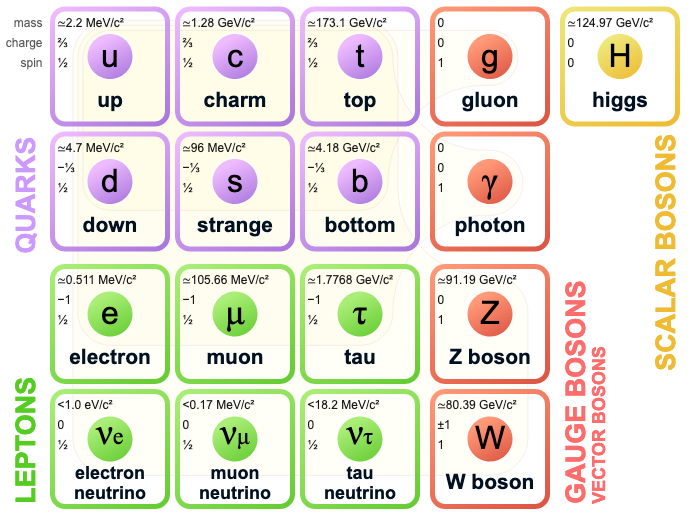
\includegraphics[width=0.8\textwidth]{Figures/1/sm.png}
    \caption{The elementary particles of the Standard Model}
    \label{fig:standardmodel}
\end{figure}

\textit{Bosons} carry integer spin, and mediate the forces via which particles interact. Massless \textit{gluons} and \textit{photons} as well as massive W and Z bosons are spin-1 vector bosons, while the Higgs Boson is a spin-0 scalar boson. The massive W and Z vector bosons are the carriers of the weak force, the photon carries the electromagnetic force, and the gluons carry the strong force binding quarks. Along with interacting with fermions via exchange, bosons are also able to interact among themselves. $W$ bosons are able to directly interact with both $Z$ bosons and and photons, as well as self-interacting. Gluons can also self-interact, but $Z$ bosons and photons cannot. The Higgs boson interacts with all massive particles, including self-interaction, and it is via their interaction with the Higgs field that massive bosons obtain their mass.

\subsection{Quantum Electrodynamics (QED)}
\textit{Quantum Electrodynamics} (QED) \cite{Feynman, schwartz, peskin} is a quantum field theory of electrodynamics and the electromagnetic force. It describes the interaction of electrically charged particles via the exchange of photons. Mathematically, QED is an abelian (commutative) gauge theory with the gauge group $U(1)$. The fundamental interactions of the theory are: the emission or absorption of a single photon by a charged particle and the creation or annihilation of a pair of charged particles. These interactions can each be represented by various orientations of the Feynman vertex shown in Figure \ref{fig:QEDvertex}.
\begin{figure}[h!]
    \centering
    \feynmandiagram [horizontal=a to b] {
    % i1 -- [fermion] a -- [fermion] i2,
    a[particle=\(\gamma\)] -- [photon] b,
    f1[particle=\(\bar{f}\)] -- [fermion] b -- [fermion] f2[particle=\(f\)],
    };
    \caption{The fundamental QED vertex.}
    \label{fig:QEDvertex}
\end{figure}

\subsection{Weak Interactions}
The weak force \cite{pdg_rev,glashow,goldstone_weinberg_salam,weinberg}, in contrast to the electromagnetic force, is mediated by the exchange of massive vector bosons $W^+$, $W^-$, and $Z$. Owing to the charge of the W bosons, and the fact in contrast to the electromagnetic force neutral fermions also interact via the weak force, there are many more possible fundamental interactions. Figure \ref{fig:EWVertices} shows the vertices corresponding three such interactions: fermions interacting with the $Z$ boson in a similar vertex to that of Figure \ref{fig:QEDvertex} shown in (a), a charged lepton and neutrino interacting with a $W$ boson shown in (b), and a quark-antiquark pair interacting with a $W$ boson shown in (c).

\begin{figure}[h!]
    \begin{subfigure}{.5\textwidth}
        \centering
        \feynmandiagram [horizontal=a to b] {
        a[particle=\(Z\)] -- [photon] b,
        f1[particle=\(\bar{f}\)] -- [fermion] b -- [fermion] f2[particle=\(f\)],
        };
        \caption{Z interaction.}
        \label{fig:EWvertexa}
    \end{subfigure}
    \begin{subfigure}{.5\textwidth}
        \centering
        \feynmandiagram [horizontal=a to b] {
        a[particle=\(W^{\pm}\)] -- [photon] b,
        f1[particle=\(\nu\)] -- [fermion] b -- [fermion] f2[particle=\(l\)],
        };
        \caption{W interaction with leptons.}
        \label{fig:EWVertexb}
    \end{subfigure}
    \newline
    % \centering
    \begin{subfigure}{1\textwidth}
        \centering
        \feynmandiagram [horizontal=a to b] {
        a[particle=\(W^{\pm}\)] -- [photon] b,
        f1[particle=\(\bar{q}\)] -- [fermion] b -- [fermion] f2[particle=\(q\)],
        };
        \caption{W interaction with quarks.}
        \label{fig:EWVertexc}
    \end{subfigure}
    \caption{Some fundamental weak interaction vertices.}
    \label{fig:EWVertices}
\end{figure}

At high energy scales, the aforementioned electromagnetic force and the weak force unify to become the electroweak interaction. Glashow, Salam, and Weinberg's Electroweak theory unites the two forces into a single $U(1) \otimes SU(2)$ gauge theory.

\subsection{Quantum Chromodynamics (QCD)}
\textit{Quantum Chromodynamics} (QCD) \cite{pdg_rev,black_book} is the theory describing the strong interaction between gluons and quarks. It is again a gauge theory, this time with the SU(3) symmetry group. There are three colour charges associated with this group, which are carried by both quarks and gluons. Each of the 8 gluons carries a unique colour charge and anti colour charge pair, while quarks carry a single colour charge. Because they carry colour charge, gluons are able to both interact with quarks and self-interact. This gives rise to several possible interaction vertices in the theory, some of which are shown in Figure \ref{fig:QCDVertices}.

\begin{figure}[H]
    \begin{subfigure}{.5\textwidth}
        \centering
        \feynmandiagram [horizontal=a to b] {
        a[particle=\(g\)] -- [gluon] b,
        f1[particle=\(\bar{q}\)] -- [fermion] b -- [fermion] f2[particle=\(q\)],
        };
        \caption{Gluon interaction with quarks.}
        \label{fig:QCDvertexa}
    \end{subfigure}
    \begin{subfigure}{.5\textwidth}
        \centering
        \feynmandiagram [horizontal=a to b] {
        a[particle=\(g\)] -- [gluon] b,
        f1[particle=\(g\)] -- [gluon] b -- [gluon] f2[particle=\(g\)],
        };
        \caption{Gluon self-interaction.}
        \label{fig:QCDVertexb}
    \end{subfigure}
    \caption{Some fundamental QCD interaction vertices.}
    \label{fig:QCDVertices}
\end{figure}

\subsection{The Higgs Boson}
Electroweak theory alone does not contain a mechanism to provide particles with mass. This contrasts with the observed reality that all fermions as well as $W$ and $Z$ bosons are in fact massive. If the lagrangian of these theories were to contain mass terms, they would lose their gauge invariance and the standard model would not be renormalizable. Instead, these particles acquire their mass through the \textit{Higgs Mechanism} \cite{Englert, Higgs1, Higgs2}.

A new Higgs Field $\Phi$ is introduced, with a Lagrangian which can be written as:
\begin{equation}
\mathcal{L}_{Higgs} = (D_{\mu}\Phi)^{\dagger}D^{\mu}\Phi + V(\Phi)
\end{equation}
Where $D_{\mu}$ is the gauge covariant derivative of the electroweak theory. In order for the Lagrangian to remain gauge invariant the Higgs potential $V(\Phi)$ must take the form:

\begin{equation}
    V(\Phi) = {\mu}^2{\Phi} + {\lambda}{\Phi}^4
\end{equation}

where $\lambda$ and $\Phi$ are free parameters. $\lambda$ is forced to be greater than 0 by requiring that the potential have a stable minimum. This leads the potential to have two different possible shapes, shown in Figure \ref{fig:higgspot}, given the sign of $\mu^2$:

\begin{enumerate}
    \item ${\mu^2 > 0}$: The trivial case of a parabolic potential with a minimum at $\Phi = 0$ arises.
    \item ${\mu^2 > 0}$: A potential with a minimum at:
    \begin{equation}
     |\Phi| = v = \sqrt{\frac{\mu^2}{\lambda}}
    \end{equation}
     arises, where $v$ is known as the vacuum expectation value. This minimum is occupied by infinitely degenerate states. This is the case that gives rise to the Higgs mechanism.
\end{enumerate}

\begin{figure}[h]
    \centering
    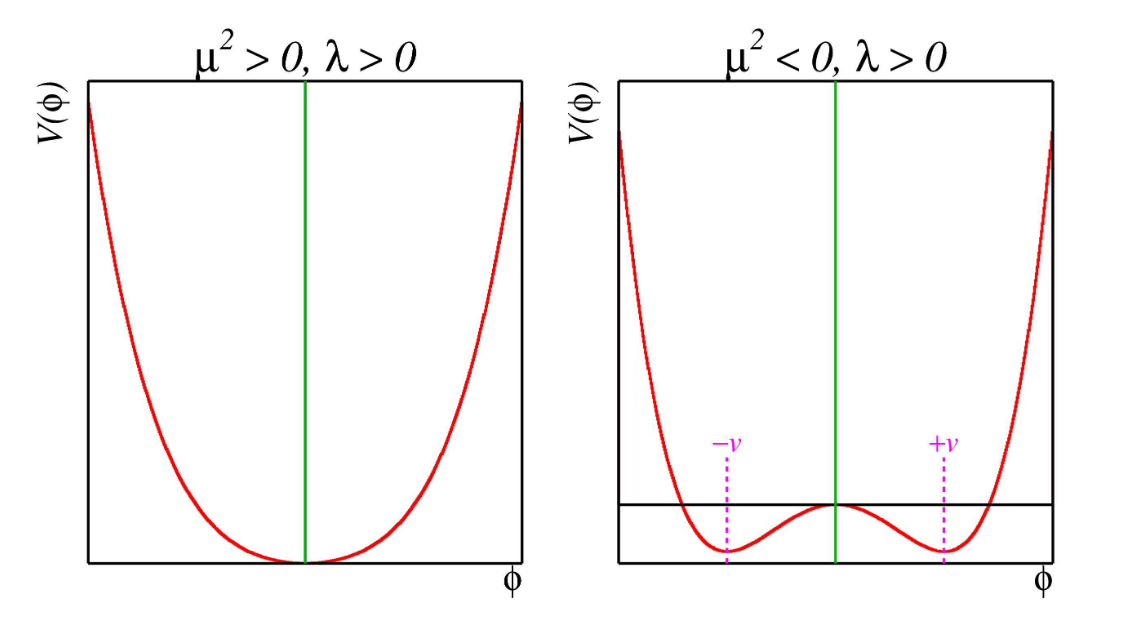
\includegraphics[width=0.8\textwidth]{Figures/1/HiggsPotential.png}
    \caption{Shapes of the Higgs Potential for different cases of $\mu^2$.}
    \label{fig:higgspot}
\end{figure}

In the second case, the ground states occupying the minimum are not equivalent under gauge transformation, which breaks the Electroweak gauge symmetry. The masses of particles are then determined by the strength of their coupling to the Higgs field.

\section{Beyond the Standard Model}
The Standard Model as described above has proven extremely robust through precise experimental testing. There are, however, many remaining questions in physics that cannot be answered within its confines. Some of those not further explored in this thesis include: whether or not there is a quantum theory of gravity that can tie it to the SM, the exact value of the neutrino masses and whether they are Majorana particles (their own antiparticles), and what the cause is of the matter-antimatter asymmetry in the universe. The fact that these questions are unanswered in the standard model tells us we must search deeper, and test beyond its limits.

\subsection{Dark Matter}
Another currently open question is the nature of dark matter. Astrophysical observations including the dynamics of galaxy clusters \cite{Zwicky} and rotational curves of galaxies \cite{Rubin} are not explained under Einstein's theory of gravitation by visible matter alone. Several theories have arisen over time to explain this discrepancy, including that Einstein's theory is not correct at galactic scales, or that these galaxies contain ordinary matter that is somehow unobservable to us.

Most evidence, however, points to the existence of a new type of matter that interacts gravitationally but not electromagnetically with ordinary matter. Perhaps the most clear evidence for this theory comes from observations of the bullet cluster \cite{Clowe}, a pair of colliding clusters of galaxies. In such a scenario, with some normal matter and some dark matter in each cluster, the matter would collide and interact, slowing it down, while the dark matter would pass through largely undisturbed. In the case of the bullet cluster, this separation is observed when comparing the distribution of mass in the galaxies measured by gravitational lensing and the distribution of normal matter in the form of galaxy plasma, measured as emitted x-ray radiation. Figure \ref{fig:bullet} shows the observed separation, with gravitational density in blue and x-ray density in pink.

\begin{figure}[H]
    \centering
    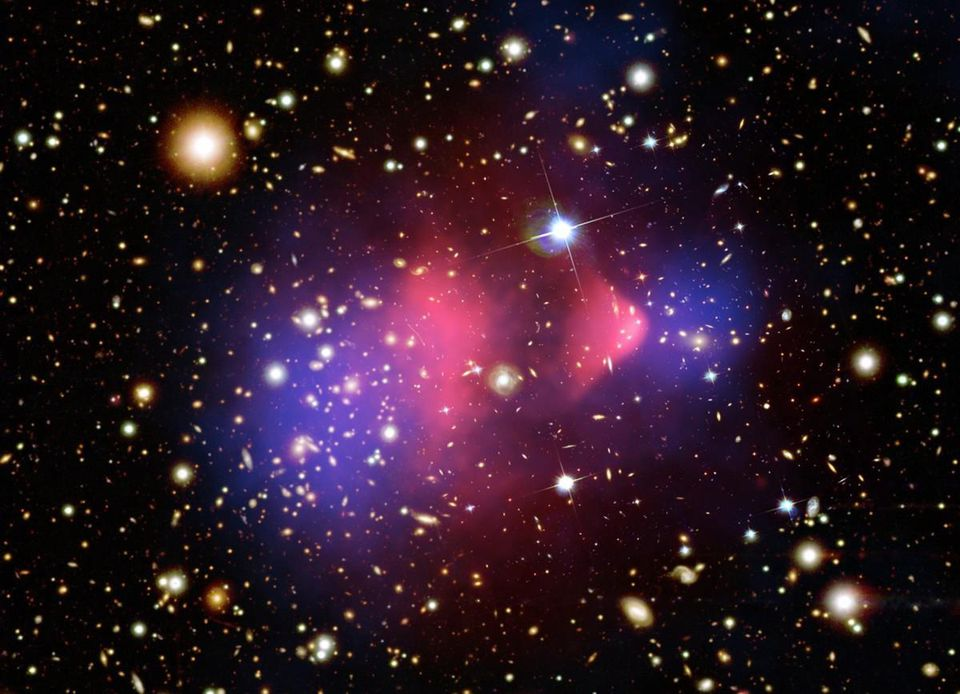
\includegraphics[width=0.7\textwidth]{Figures/1/bullet.png}
    \caption{The bullet cluster showing separation of x-ray density (pink) and gravitational density (blue).}
    \label{fig:bullet}
\end{figure}

\subsection{Dark Higgs Boson Model}
\label{subsection:dh_model}
This work involves a search for dark matter produced in association with a new hypothetical scalar ``dark Higgs" boson $s$\footnote{In this work, $s$ will refer  to the dark Higgs boson and not the strange quark, unless otherwise spefcified} \cite{Hunting}. In this model the dark matter particle $\chi$ is a majorana fermion, who's mass is generated by a Higgs mechanism in the dark sector. This also generates the new $s$ particle. If the mass of $s$ is less than that of $\chi$ then the relic density is set by the process $\chi\chi \rightarrow ss$, followed by the decay of $s$ to standard model partices. The addition of a further paricle, such as a massive $Z'$ boson allows this model to be probed at a collider.

The model proposes that the dark matter particle $\chi$ obtains its mass from the vacuum expectation value (vev) $w$ of a new Higgs field $S$. A new $U(1)'$ gauge group is proposed, under which $S$ carries a charge $q_s$. As a result, the vev $w$ of $S$ breaks the gauge symmetry, and through this mechanism the mass of the corresponding $Z'$ boson is generated. Additionally, the dark matter particle $\chi$ couples to the $Z'$ boson, allowing all particles in the new dark sector to interact. This gives rise to the renormalizable interaction Lagrangian, which can be written in terms of four independent parameters $m_{\chi}$, $m_{Z'}$, $m_{s}$, and $g_{\chi}$:

\begin{equation}
\mathcal{L}_{\chi} = -\frac{1}{2}g_{\chi}Z'^{\mu}\bar{\chi}\gamma^5\gamma_{\mu}\chi - g_{\chi}\frac{m_{\chi}}{m_{Z'}}s\bar{\chi}\chi + 2g_{\chi}Z'^{\mu}Z'_{\mu}(g_{\chi}s^2 + m_{Z'}s)
\end{equation}

where $m_{\chi}$ is the mass of the dark matter particles, $m_{Z'}$ is the mass of the $Z'$ boson, $m_{s}$ is the mass of the dark higgs, and $g_{\chi}$ is the dark matter coupling constant.

Additionally, the coupling of the $Z'$ boson to standard model quarks is described by the Lagrangian:

\begin{equation}
\mathcal{L} = -g_qZ'^{\mu}\bar{q}\gamma_{\mu}q
\end{equation}

where $g_q$ is the coupling constant between $Z'$ and quarks.

A final free parameter $\theta$ is the non-zero mixing angle between the SM Higgs boson and the dark Higgs boson. The dark Higgs obtains its couplings to standard model particles through this mixing, and therefore shares the same standard model decay branching fractions as the SM Higgs boson.

For the analysis described in this work the free parameters are set as:

\begin{itemize}
    \item $g_{\chi} = 1$
    \item $m_{\chi} = 200 GeV$
    \item $m_{Z'}$ allowed to vary
    \item $m_s$ allowed to vary
    \item $g_q = 0.25$
    \item $\theta = 0.01$
\end{itemize}

The values of $g_{\chi}$ and $g_{q}$ were chosen to facilitate comparison with other LHC searches with similar models, which traditionally use the values selected. The value of $\theta$ was chosen to match that of \cite{Hunting}. Its precise value is not relevant to this search, but it is sufficiently large that the dark Higgs decays promptly to standard model states and does not create a displaced vertex. The varied values $m_s$ and $m_{Z'}$ form the parameter space covered by this search.

	\startchapter{The Large Hadron Collider and the ATLAS Experiment}
\label{chapter:lhcatlas}

The \textbf{Large Hadron Collider (LHC)} is the world's largest and most energetic proton-proton collider. It forms a 27 km circular ring beneath Switzerland and France, with its origin at the \textbf{Conseil Européen pour Recherche Nucléaire (CERN)} in Geneva. It began operation in 2008, and since then has collided over $10^{15}$ particles. The collider houses four major experiments: ALICE, ATLAS, CMS, and LHCb, along with several smaller projects. ALICE (A Large Ion Collider Experiment) studies heavy ion collisions, while LHCb (Large Hardon Collider beauty) specializes in studying the physics of the bottom quark. \textbf{ATLAS (A Toroidal LHC ApparatuS)} and CMS (Compact Muon Solenoid) are both general purpose experiments designed to study a wide range of interactions resulting from high-energy proton-proton collisions. This work uses data collected by the ATLAS experiment, and a description of the LHC accelerator and ATLAS detector follow in Sections \ref{section:lhc} and \ref{section:atlas}.

\section{The Large Hadron Collider}
\label{section:lhc}
Built between 1998 and 2008, the LHC \cite{LHCDesign} began colliding protons in 2010 at a center-of-mass energy of 7 TeV, and most recently from 2015 to 2018 collisions occured at 13 TeV. Successfully colliding particles at this energy is an immense technical challenge which is achieved by the many technologies of the LHC and its accelerator complex.

In order to reach a beam energy of 6.5 TeV, protons are slowly stepped up through a chain of accelerators before reaching the LHC. They begin their journey as hydrogen atoms, stripped of their electrons before being accelerated to an energy of 50 MeV by the Linac2 linear accelerator. Following this the Proton Synchrotron Booster (PSB) accelerates them to 1.4 GeV, passing them to the Proton Synchrotron (PS) and the Super Proton Synchrotron to be accelerated to 25 and then 450 GeV. Finally, beams are split into clockwise and counterclockwise directions and injected into the LHC where they are accelerated to their final 6.5 TeV energy. The CERN accelerator complex, including this injection system as well as surrounding experiments is shown in Figure \ref{fig:lhc_injector}.

\begin{figure}[h!]
    \centering
    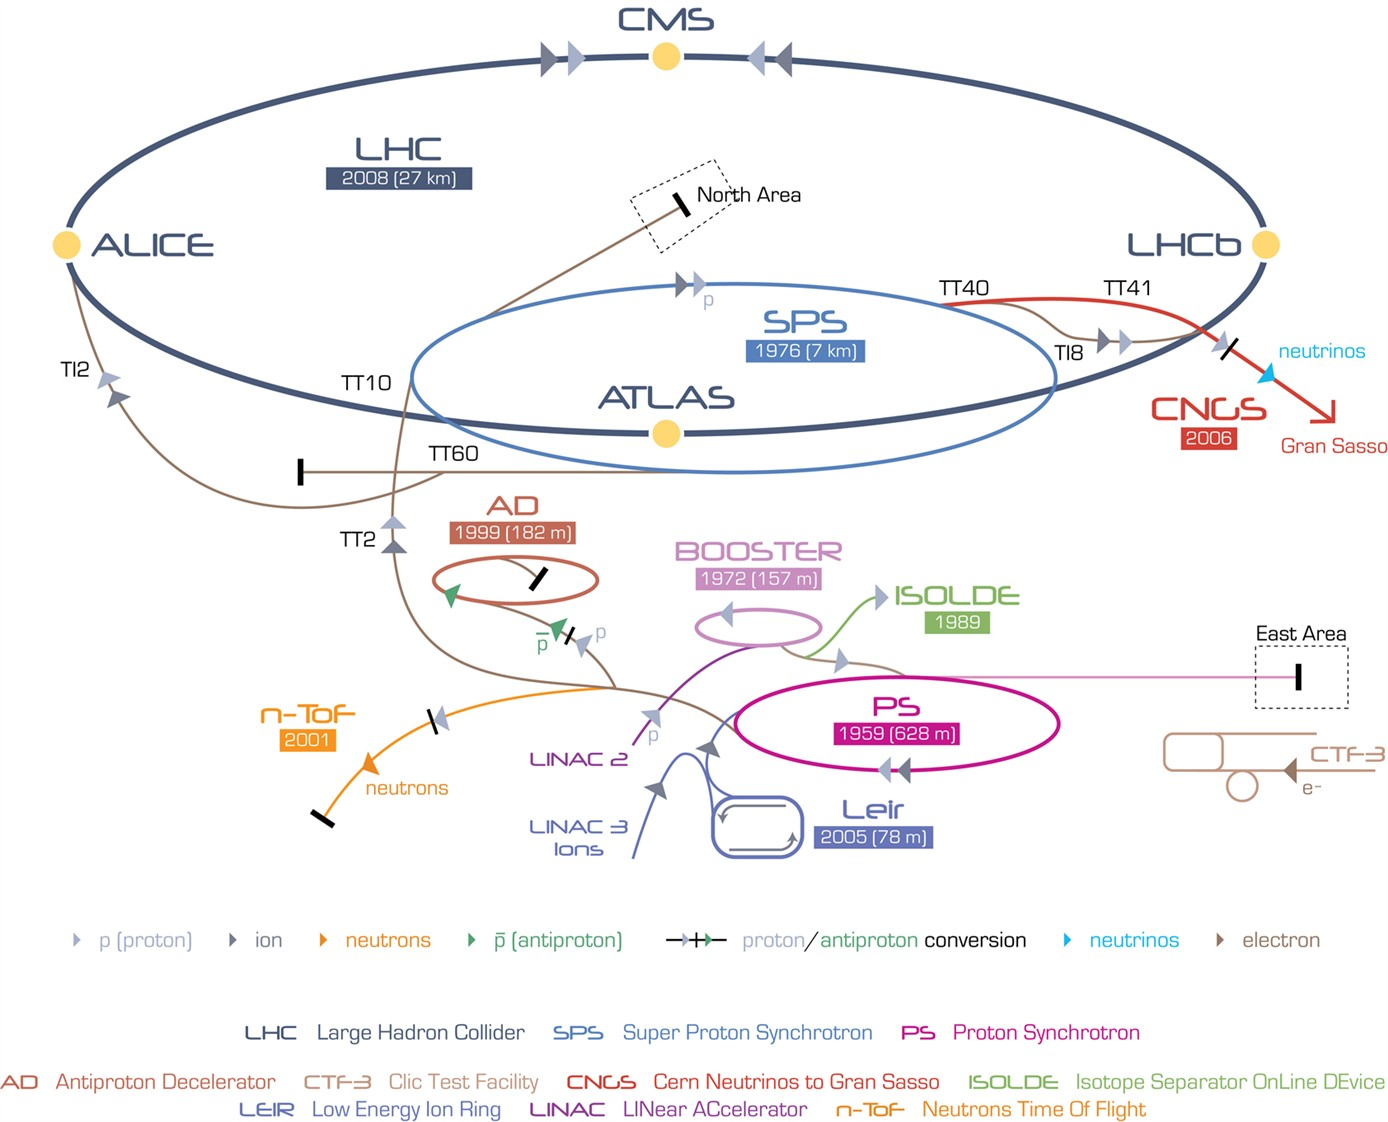
\includegraphics[width=0.8\textwidth]{Figures/2/cern_complex.png}
    \caption{Overview of the CERN accelerator complex, including the LHC injector system and surrounding experiments.}
    \label{fig:lhc_injector}
\end{figure}

The acceleration of the protons is achieved by radio-frequency cavities. These cavities contain a resonant electromagnetic field oscillating at 400 MHz, which is applied to particles passing through. The LHC contains 8 cavities per beam, with each providing a maximum of 2 MV of potential, so each proton can recieve up to 16 MeV of energy per lap. As a result it takes millons of laps over a period of around 20 minutes for a proton injected at 450 GeV to reach its collision energy of 6.5 TeV.  These RF cavities also serve to keep each beam in bunches of $1.15 \times 10^{11}$ protons spaced at intervals of just 25 ns.

The crown jewel of LHC technology is its magnets. 1,232 superconducting NbTi dipole magnets kept at 1.9 K, each spanning 14.3 m and weighing 35 tonnes, create an 8.3 Tesla magnetic. This field lies perpendicular to the beam path, bending it to its desired route. The bending dipole magnets are complemented by 392 quadrupole magnets that focus the beams to a small aperture, and many higher-order multipole magnets which provide small beam corrections.

Allong with the collisional energy of the accelerated particles, the other most important measure of a particle acceletator is the luminosity it achieves. \textbf{Luminosity ($\mathcal{L}$)} is used to determine the rate ($R$) at which a given interaction occurs using:
\begin{equation}
R = \mathcal{L}\sigma
\end{equation}
where $\sigma$ is the cross-section of the desired interaction. As a result, when searching for rare processes, a obtaining a high luminosity is crucial.

The integrated luminosity, $L$, gives the total number of interactions over a period of time, and is defined as:
\begin{equation}
L = \int \mathcal{L}\, dt
\end{equation}
At the LHC, the luminosity is controlled by the number of bunches circulating $n_b$, the frequency of revolution $f_r$, $N_{1,2}$ the number of particles in each colliding bunch, and the cross sectional area of the colliding beams. This results in the equation:
\begin{equation}
\mathcal{L}  = \frac{ f_rn_bN_1N_2 }{4\pi\sigma_x\sigma_y}R_{\phi}
\end{equation}
where $R_{\phi}$ is a geometrical loss factor caused by the beams crossing at an angle, and $\sigma_{x,y}$ are the horizontal and vertical widths of the beams, which are estimated to have a Gaussian profile. The LHC currently has a nominal peak luminosity of $\mathcal{L} = 10^{34} cm^{-2}s^{-1}$.

\section{The ATLAS Experiment}
\label{section:atlas}

The ATLAS experiment \cite{ATLASDesign} uses the LHC in combination with the general-purpose ATLAS detector to test a broad range of SM and BSM predictions. Together with the CMS experiment, its greatest achievement to date was the detection and discovery of the SM Higgs boson in 2012 \cite{HiggsDiscovery}.

\begin{figure}[H]
    \centering
    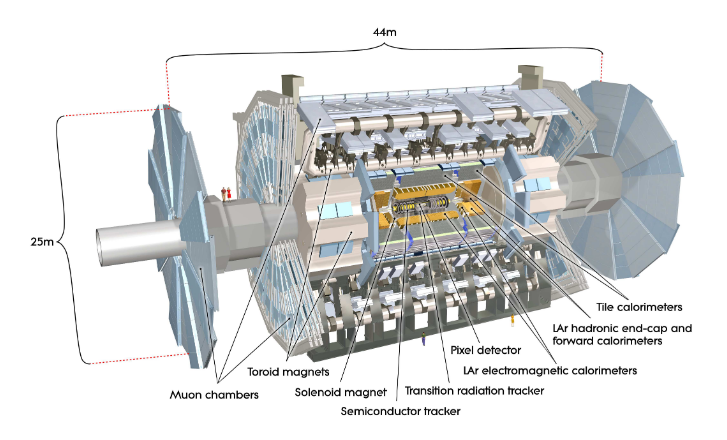
\includegraphics[width=0.8\textwidth]{Figures/2/ATLASDetector.png}
    \caption{A cut-out overview of the ATLAS detector and main components. Diagram from \cite{ATLASDesign}.}
    \label{fig:atlasdec}
\end{figure}

The ATLAS detector, an overview of which is shown in Figure \ref{fig:atlasdec}, is comprised of several layers, which work in tandem to detect many diverse particles. From inner-most to outer-most the layers are:

\begin{itemize}
    \item the \textbf{inner detector}, with excellent angular resolution to track charged particles,
    \item the \textbf{electromagnetic calorimeters}, designed primarily to measure the energy and position of electrons and photons,
    \item the \textbf{hadronic calorimeters} designed to measure the energy and position of hadrons,
    \item the \textbf{muon spectrometer}, to track and measure muons.
\end{itemize}

When combined with the electronics required to read and trigger on measurements, the entire detector weighs over 7000 t and measures 44 m long by 25 m wide and high. Its barreled shape with end caps covers nearly the full solid angle. The following sections will describe the layout and operations of the ATLAS detector in more detail.

\subsection{Inner Tracking Detector}
The ATLAS inner detector tracks the direction and momentum of charged particles immediately after leaving the interaction point. A 2 T superconducting solenoid surrounds the inner detector, bending charged particles with the Lorentz force, allowing their momentum to be determined from the curvature of their path. Within the inner detector, there are three separate sub-detectors: the \textbf{Pixel Detector}, the \textbf{Semiconductor Tracker (SCT)}, and the \textbf{Transition Radiation Tracker (TRT)}. A cutout view of the detector is shown in Figure \ref{fig:atlasinner}.

\begin{figure}[H]
    \centering
    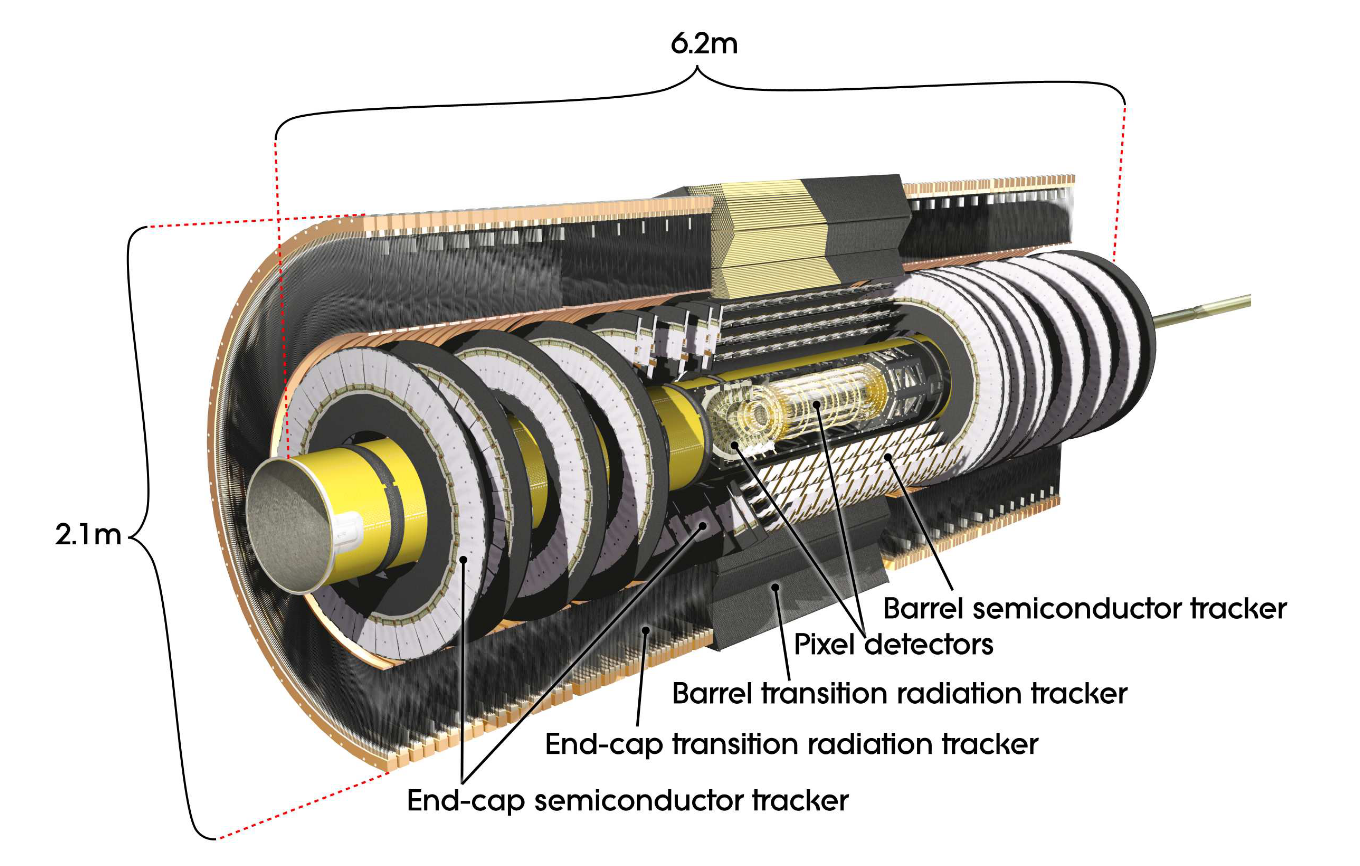
\includegraphics[width=0.8\textwidth]{Figures/2/InnerDetector.png}
    \caption{A cut-out view of the ATLAS inner detector. Diagram from \cite{ATLASDesign}.}
    \label{fig:atlasinner}
\end{figure}

The Pixel Detector consists of an array of 1744 pixel sensors, each containing 47232 silicon pixels, mostly measuring 50x400 $\mu m^2$. They are arranged into three cyclindrical layers in the barrel and three disk-shaped layers on each end. The high granularity of these detectors ensures strong angular resolution, providing prescise measurements of vertex location and track momentum. Notably, this detector must be very radiation-hard in order to maintain performace over the detector lifespan in an area that recieves an immense radiation dose from the high particle flux.

Though it would be desireable, it would not be feasible to extend the high-resolution pixel detector because of the high cost and signal readout volume. As a result, in the SCT the point-like pixels are extended into silicon strip detectors, which are laid in pairs at an angle of 40 mrad to each other to allow measurements in two dimensions. The SCT is made up of four concentric cylindrical layers in the barrel and two disk-shaped layers on each end-cap.

The TRT is the final component of the component of the inner detector.  It consists of approximately 300000 drift tubes filled with majority Xenon gas, with the walls kept at -1.5 kV and a central wire at ground. When particles pass through the tubes, the gas is ionized and the resulting electrons drift to the centre where the signal is amplified. Additionally, the gaps between TRT straws are filled with polymer fibres (in the barrel) or foils (in the end caps). As a result, highly relativistic particles create transition radiation at the material interfaces, which aids with electron identification.

\subsection{Calorimeters}
The ATLAS calorimeter system measures the energy and positions of both charged and neutral particles after they leave the inner detector. In addition to measuring the energy of particles, the calorimeters must contain enough material to stop the vast majority of particles (with the exception of muons and undetected neutrinos) from reaching the muon spectrometers. To acheive this, high-density passive layers interact with passing particles and cause them to decay into showers, dispersing their energy. These layers are interleaved with active layers that detect the decaying showers to measure particle energy.

\begin{figure}[H]
    \centering
    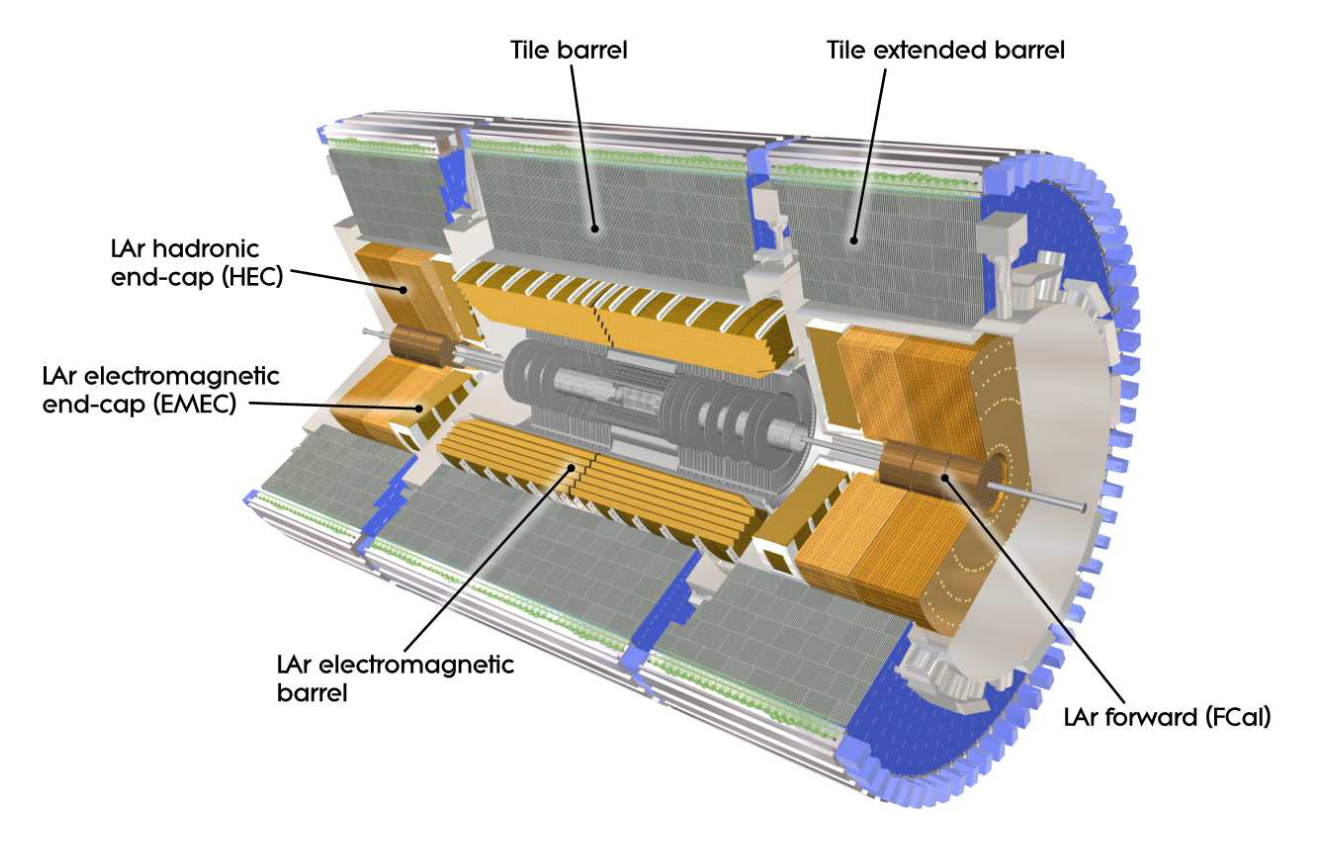
\includegraphics[width=0.8\textwidth]{Figures/2/Calo.png}
    \caption{A cut-out view of the ATLAS calorimeter system. Diagram from \cite{ATLASDesign}.}
    \label{fig:atlascalo}
\end{figure}

The ATLAS calorimeters can be categorized into electromagnetic (EM) calorimeters which measure the energy of electrons and photons and hadronic calorimeters which prmarily measure the energy of hadrons. ATLAS uses a combination of two different calorimeter technologies to form these detectors. In the end-cap and forward regions Liquid Argon (LAr) is used as the active layer in both the hadronic and EM calorimeters, while in the barrel region plastic scintillating tiles are employed in the hadronic calorimeter. Figure \ref{fig:atlascalo} depicts the layout of the ATLAS calorimeter system.

\subsubsection{Electromagnetic calorimeters}
The electromagnatic LAr calorimeter lies just outside the solenoid surrounding the inner detector. Layers of lead are used as the passive material. In the lead, electrons and photons interact with the closely spaced atoms, initiating a cascading shower of decays. The charged electrons in the shower pass through the active layers and ionize the LAr inside. The electrons and ions then drift across the 2 kV difference to opposite electrodes, where they are amplified into an electrical signal.

Like the inner detector, the LAr EM calorimeter can be divided into an \textbf{Electromagnetic Barrel (EMB)} calorimeter and two \textbf{Electromagnetic End-Cap (EMEC)} calorimeters. In the barrel region, the layers are placed together in a folded accordion-like geometry to create uniformity and allow easy electronic readout. The barrel and end-cap regions are 53 cm and 63 cm thick respectively, and cover a minimum of 22 and 24 radiation lengths ($X_0$), keeping shower leakage to a minimum.

\subsubsection{Hadronic Calorimeters}
In the end cap regions, the \textbf{Hadronic End-Cap (HEC)} calorimeter shares a similar design to the EM LAr calorimeters, but with copper as the passive absorbing material between active layers. In the barrel region, the hadronic calorimetry is performed by the \textbf{Tile Calorimeter} with plastic scintillators as the active detectors. Particle showers passing through the plastic tiles produce scintillating light, which is directed to photomultipliers to be converted to an electrical signal. In the tile calorimeter, steel is the passive material laid between active layers. The depth of the combination of electromagnetic and hadronic calorimeters is important to prevent particles from punching through to the background-sensitive muon spectrometer. The total thickness, including supporting materials, is approximately 11 interactions lengths, which keeps punch-through below the levels of irreducible backgrounds in the muon spectrometer and also ensures an accurate measurement of $E^{miss}_T$ as very little energy escapes measurement.

The final calorimeter in the ATLAS detector is the \textbf{Forward Calorimeter (FCal)}, located nearest the beam path. It has three layers of passive absorbing metals: an inner copper layer optimized for electromagnetic measurements and two outer tungsten layers to measure hadronic interactions. It too employs liquid argon as the active material, this time in a matrix of longitudinal channels parallel to the beam line.

\subsection{Muon Spectrometers}
After the calorimeters have stopped the vast majority of particles exiting the interaction point, muons and neutrinos remain undetected. The ATLAS experiment does not directly detect neutrinos, and instead reconstructs them from missing transverse momentum, but muons are measured by the muon spectrometer. A diagram of the muon system is shown in Figure \ref{fig:muon_system}. The centerpiece of this system is an arrangement of three air-core toroidal magnets, a barrel toroid and two end-cap toroids. Each toroid consists of eight coils in loops in a radially symmetric pattern around the beam line. Together they form a 4 T magnetic field to bend muons.

\begin{figure}[H]
    \centering
    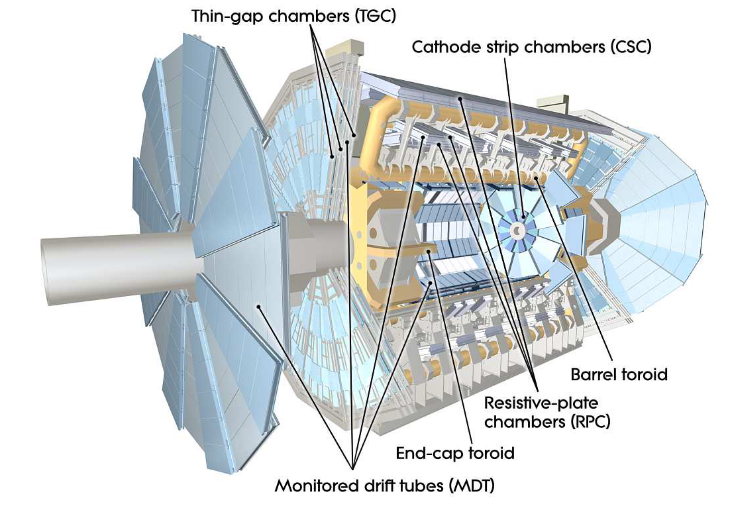
\includegraphics[width=0.8\textwidth]{Figures/2/muon_system.png}
    \caption{A cut-out view of the ATLAS muon spectrometer system. Diagram from \cite{ATLASDesign}.}
    \label{fig:muon_system}
\end{figure}

Four different detector types are used to measure the muons. \textbf{Monitored Drift Tubes (MDTs)} are pressurized gas drift tubes that collect ionized electrons to measure track coordinates in the bending direction of the magnetic field. They are supplemented by finer-grained and more radiation-hard \textbf{Cathode Strip Chambers (CSCs)} at $|\eta | > 2$. \textbf{Resistive Plate Chambers (RPCs)} and \textbf{Thin Gap Chambers (TGCs)} measure the muon track coordinares in the direction orthogonal to the magnetic bending direction, and are also used by the trigger system to provide bunch-crossing indentification and $p_T$ thresholds.

\subsection{Trigger and Data Acquisition}
The ATLAS detector can see as many as 1.7 billion proton-proton collisions per second, but to save and process all of the information from each collision would require a prohibitive amount of readout electronics, computing power, and storage space. Instead, the trigger system quickly selects events based on key observables to slim down the data.  On the detector itself, the \textbf{Level-1 (L1) trigger} uses custom electronics within the detector, and works with reduced granularity information from the muon chambers and calorimeters to select potentially interesting events with high-$p_T$ objects or high $E^{miss}_T$. The detector readout systems can handle a maximum acceptance rate of 100 kHz from the L1 trigger. The \textbf{Level 2 (L2) trigger} is outside the detector and uses traditional computing resources. It takes regions of interest where the L1 trigger finds interesting objects and reconstructs them more fully to further reduce the event rate below 3.5 kHz. Together with the L2 trigger, the \textbf{event filter} forms the second half of the \textbf{High-Level Trigger (HLT)}. At this stage, events are fully reconstructed before being further filtered to a rate of approximately 200 Hz to be analyzed offline.

	\startchapter{Analysis Preparation}
\label{chapter:ana_prep}

\section{Signal Model}
This work concerns a search for dark matter produced in association with a dark Higgs boson as described in Subsection \ref{subsection:dh_model}.  The dark Higgs boson, $s$, then decays to standard model particles with the same branching ratios as a standard model Higgs boson of variable mass, as shown in Figure \ref{fig:HiggsBR}. At low $s$ mass, this is dominated by a decay to a pair of $b$ quarks, is currently being studied via a reinterpretation of the ATLAS search for dark matter produced in association with a standard model Higgs boson decaying to $b\bar{b}$ in \cite{monos_bb}. At $s$ masses above 160 GeV, however, the decay to a pair of $W$ bosons, shown in Figure \ref{fig:dh_feynman}, becomes kinematically available on-shell. Even slightly below this threshold, $s$ decays to $WW$ are the dominant process. The pair of $W$ bosons decay rapidly, and are not detected as final state particles by the ATLAS detector. Instead, they each decay either to hadronic ($q\bar{q}$) or leptonic ($l\nu$) final states. A search in the fully hadronic channel, with both $W$ decaying to $q\bar{q}$, is complete (see \cite{had_analy}), and this work focuses on the semileptonic decay channel with one $ W \rightarrow q\bar{q} $ and one $ W \rightarrow l\nu $. When both analyses are complete, the results will be statistically combined.

\begin{figure}[H]
    \centering
    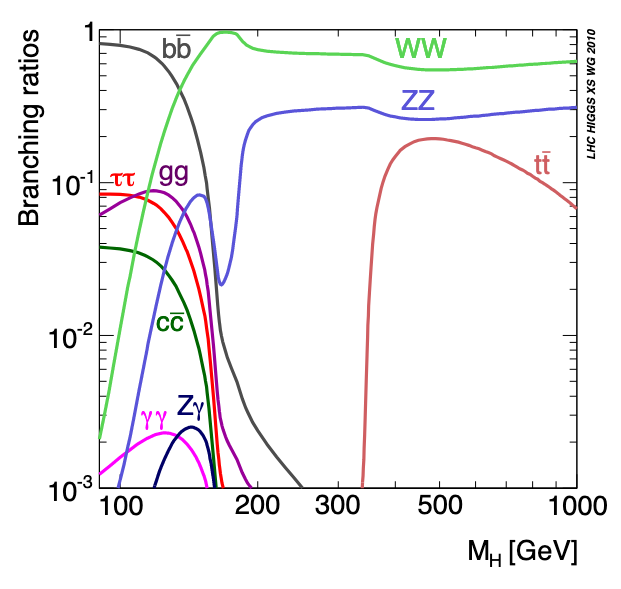
\includegraphics[width=0.8\textwidth]{Figures/3/HiggsBR.png}
    \caption{Branching fractions for a SM Higgs boson as a function of the Higgs boson mass \cite{Higgs_BR}.}
    \label{fig:HiggsBR}
\end{figure}

\begin{figure}[H]
    \centering
    \feynmandiagram [horizontal=a to b] {
    i1[particle=\(q\)] -- [fermion] a -- [fermion] i2[particle=\(q\)],
    a -- [boson, edge label=\(Z'\)] b,
    b -- [boson, edge label=\(Z'\)] c,
    b -- [scalar, edge label=\(s\)] d,
    f1[particle=\(\chi\)] -- [fermion] c -- [fermion] f2[particle=\(\chi\)],
    f3[particle=\(W\)] -- [boson] d -- [boson] f4[particle=\(W\)],
    f2 -- [opacity=0.0] f3
    };
    \caption{Dark Higgs boson decay}
    \label{fig:dh_feynman}
\end{figure}

In the ATLAS detector, this signal signature will be characterized by a single lepton in the final state from the $ W \rightarrow l\nu $ decay, along with a pair of jets from the $ W \rightarrow q\bar{q} $ decay and a strong missing transverse momentum signature from the dark matter particles and neutrino.

\section{Monte Carlo Production and Data}
\label{section:mc_prod}
In order to search for a signal such as the one described above, it is necessary to form a prediction which can be compared with data from the ATLAS detector. In order to achieve this, simulated data is produced using Monte Carlo (MC) generators according to standard model predictions. This represents ``background" data, or what we would expect to see if the signal process did not exist. Added to this, signal MC samples are produced according to the signal model. Then, after isolating for an area of phase space that would be rich in signal events, the ATLAS data can be compared with the simulated data with or without signal events to make statistical conclusions about the likelihood of the existence. The following sections will detail the MC and data samples prouduced for ths analysis.

\subsection{Signal MC}
\label{subsection:mc_signal}
Signal samples are produced using the model and parameter choices outlined in subsection \ref{subsection:dh_model}. They are produced by calculating the hard process cross-section at leading order (LO) using \mgamc 2.7.2 \cite{MadGraph} interfaced with \pythia 8.230 \cite{Pythia} for parton shower modelling. The CKKW-L \cite{CKKW} procedure with a matching scale of $min(m_s/4, 40~\text{GeV})$ is used to prevent overlap between the cross-section matrix element and parton shower. Two separate signal grids were produced, with the second covering an expanded parameter space. In the first, \mgamc is used with the NNPDF30 LO PDF set with $\alpha_s = 0.13$ \cite{PDF30}, while in the second \mgamc is used with the NNPDF30 NLO PDF set with $\alpha_s = 0.118$ \cite{PDF30}. The signals studied span a parameter space in \ms and \mZp with samples produced at the mass points shown in Figure \ref{fig:signal_grid}.

\begin{figure}[H]
    \centering
    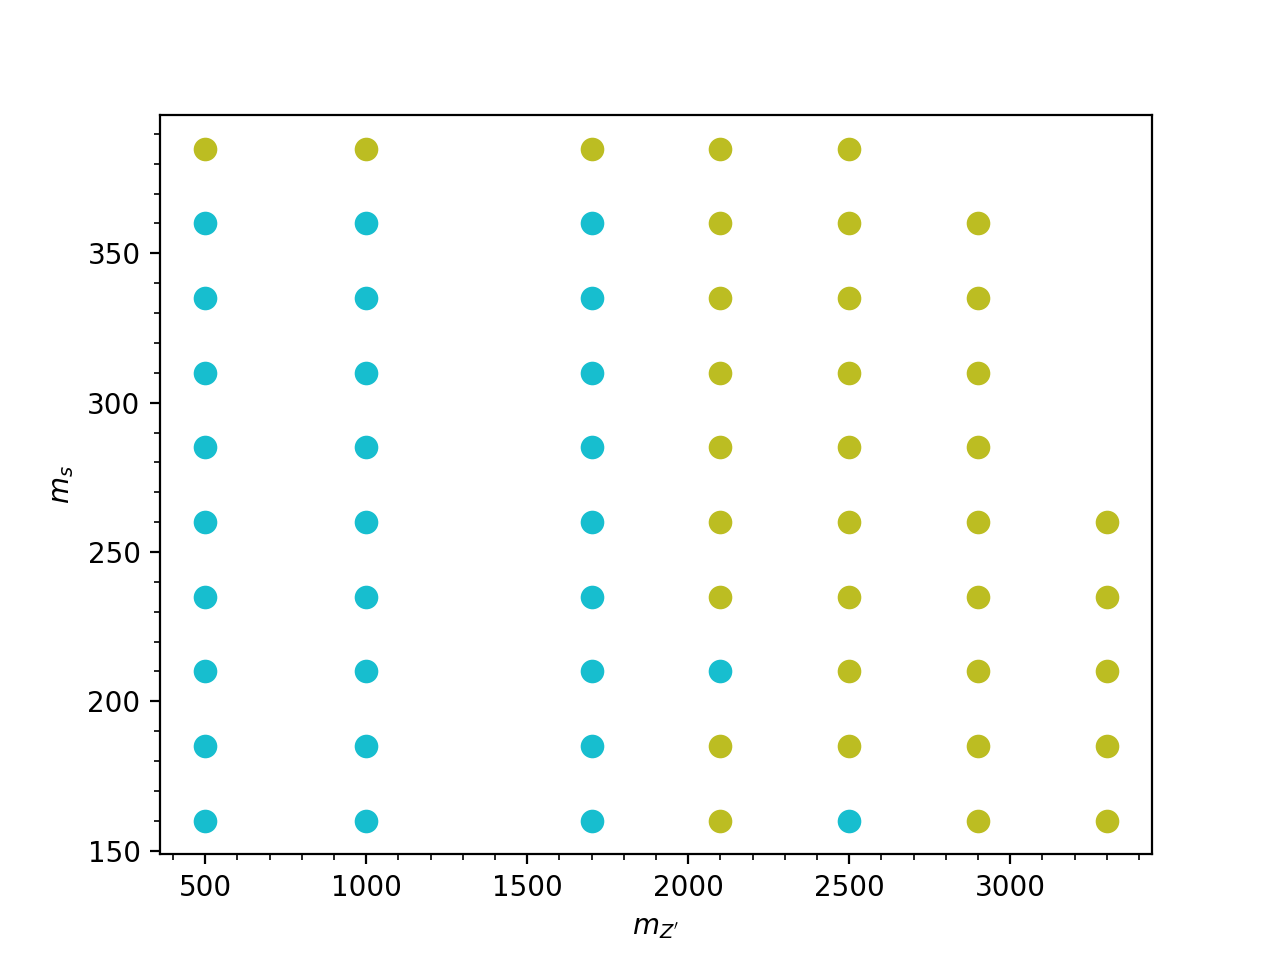
\includegraphics[width=0.8\textwidth]{Figures/3/SignalGrid.png}
    \caption{Signal point locations in \ms vs. \mZp parameter space. Blue points represent the original signal grid while green points are added in the second signal grid.}
    \label{fig:signal_grid}
\end{figure}

\subsection{Background MC}
\label{subsection:mc_bkg}
The dominant and sub-dominant SM backgrounds for this analysis are:
\begin{itemize}
    \item \wjets events, containing a single $W$ boson and 1 or more jets,
    \item \ttbar, containing with a top and anti-top pair, and
    \item di-boson events, containing a pair of vector bosons.
\end{itemize}
Additionally, \zjets, tri-boson, and single-top quark\footnote{In some plots in this work single-top quark events are denoted by the short form ``stop". This is not to be confused with a supersymmetric partner of a top-quark often referred to as a ``stop".} events make non-negligible background contributions. All background contributions are estimated using MC simulated data, and the \wjets and \ttbar backgrounds are further constrained using data-driven control regions.

\subsubsection{\vjets, Di-boson, and Tri-boson}
Two distinct sets of \wjets and \zjets (\vjets) background samples are used. The samples are simulated with the \sherpa v2.2 MC generator \cite{Sherpa} with up to two additional parton emissions at NLO or four additional parton emissions at LO accuracy \cite{VJets}\cite{VJets_mW}. Merging of parton showers with matrix elements is acheived using CKKW \cite{CKKW} matching with the MEPS@NLO prescription extending this to NLO \cite{MEPS}. The NNPDF30 NNLO PDF set is used \cite{PDF30}.

The difference is that first samples are produced using \sherpa v2.2.1, and the second with \sherpa v2.2.10. As well, additional statistics-enhanced \wjets samples are added to the second set with $m_W > 120$ GeV \cite{VJets_mW}. This greatly increases the number of simulated events in this small section of phase space that is important to this analysis. Overlap removal in $m_W$ is performed between these mass-enhanced samples and the other \wjets samples.

Di-boson and tri-boson samples are similarly generated with only a single set using either \sherpa v2.2.1 or v2.2.2 depending on the process, and CKKW matching is again used to merge parton shower and matrix element simulation.

\subsubsection{\ttbar and single-top}
MC samples for the \ttbar and single-top standard model background process are modelled using the \powhegbox v2 \cite{Powheg} generator, which gives matrix elements at NLO in the strong coupling constant $\alpha_s$. This uses the NNPDF30 NLO PDF set \cite{PDF30}. Similar to the signal samples, this is combined with \pythia 8.230 \cite{Pythia} for parton shower modelling using the NNPDF23 LO PDF set \cite{PDF23}.

\subsection{Data}
This analysis uses data from the full Run-2 period, i.e. from 2015-2018, with individual runs selected using the good runs lists:
{ \scriptsize
\begin{itemize}
	\item \GRLa
	\item \GRLb
	\item \GRLc
	\item \GRLd
\end{itemize}
}
This results in a total integrated luminosity of 138.5 fb$^{-1}$.

\subsubsection{MC Scaling to Match Data Luminosity}
\label{subsubsection:mc_scaling}
The events in MC simulated samples above must be re-weighted in order to match the total integrated luminosity of the ATLAS data used. In order to achieve this, the weight of each MC event is given by:
\begin{equation}
weight  = \frac{ \sigma \times (138.5~fb^{-1}) \times (k) \times (filt_{eff}) \times (GenWeight) \times (wf)}{\sum_{Events~in~AOD} GenWeight }
\end{equation}
where
\begin{itemize}
\item \sigma~is the cross section for the simulated process in fb,
\item $k$ is the k-factor, which corrects for the omission of higher-order terms in event generation,
\item $filt_{eff}$ is the filter efficiency, the fraction of events passing any filters applied during event generation to emphasize a certain phase space,
\item GenWeight is the generator weight from MC production,
\item and $wf$ is a set of weight factors given by:
\begin{equation}
wf = EleWt \times MuoWt \times JetWtJVT \times prwWt
 \times TriggerWts \end{equation}
where the various weights apply small corrections from the generation and reconstruction process.
\end{itemize}


\section{Object Definition}
\label{section:objects}
Once events have been simulated or produced in the ATLAS detector, the information contained in them must be reconstructed into objects which can be analyzed. These objects represent particles or groups of particles, and are used to fully or partially reconstruct events and search for signal signatures. The following section will detail the definition of physics objects used in this analysis.

\subsection{Muons}
\label{subsection:muons}
From the ATLAS detector, muons are reconstructed from measurements in the Inner Detector and the Muon Spectrometer. For this analysis, two different definitions of muon candidates are used. ``\textit{Baseline}" muons use slighlty looser selection criteria than ``\textit{signal}" muons, which are designed for high purity. \textit{Baseline} muons are selected using the \textit{Loose} identification criteria as defined in \cite{muon_wp}, which is designed to maximize efficiency. \textit{Signal} muons, meanwhile, use the \textit{Medium} identification criteria, and must also be isolated from other signatures according to the \textit{Tight} track-based working point, with variable radius dependent on \pT. Additionally, all muons are rejected if they are considered ``badly reconstructed" or ``cosmic", and track-to-vertex association cuts are applied. Table \ref{tab:muon_criteria} summarizes the muon selection criteria.

\begin{table}[H]
\centering
\caption{Muon object definition criteria}
\label{tab:muon_criteria}
\begin{tabular}{l l l}
\toprule
\textbf{Criterion} & \textbf{Baseline Muon} & \textbf{Signal Muon} \\
\midrule
Identification & \verb|Loose| & \verb|Medium| \\
Isolation & - & \verb|TightTrackOnly_VarRad| \\
\midrule
Pseudorapidity & \(\abs{\eta} < 2.7\) & \(\abs{\eta} < 2.5\) \\
\pT & \(\pT > \unit[7]{\GeV} \) & \(\pT> \unit[7]{\GeV} \) \\
\midrule
Veto & Cosmic or Bad & Cosmic or Bad \\
\midrule
\multirow{2}{*}{Track-to-vertex association} & \(\abs{d_0 / \sigma_{d_0}}  < 3 \) & \( \abs{d_0 / \sigma_{d_0}}  < 3 \) \\
	& \( \abs{\Delta z_0^\textrm{BL} \sin \theta} < \unit[0.5]{mm} \) & \( \abs{\Delta z_0^\textrm{BL} \sin \theta} < \unit[0.5]{mm} \) \\
\bottomrule
\end{tabular}
\end{table}

\subsection{Electrons}
\label{subsection:electrons}
Electrons are reconstructed by associating energy deposits in the EM calorimeter with tracks in the inner detector. Similar to muon candidates, two different definitions are used, with ``\textit{baseline}" electrons requiring slightly less selective criteria than ``\textit{signal}" electrons. \textit{Baseline} and \textit{signal} electrons are selected using a likelihood-based identification described in \cite{e_wp}. \textit{Signal} electrons require the medium identification criteria, while \textit{baseline} electrons requre the loose criteria as well as a hit in the innermost layer of the pixel detector. Additionally, \textit{baseline} and \textit{signal} electrons must both satisfy the fixed-cut \textit{Loose} isolation requirement. Like for muons, track-to-vertex association cuts are also applied. Table \ref{tab:electron_criteria} summarizes the electron selection criteria.

\begin{table}[H]
\centering
\caption{Electron object definition criteria}
\label{tab:electron_criteria}
\begin{tabular}{l l l}
\toprule
\textbf{Criterion} & \textbf{Baseline Electron} & \textbf{Signal Electron} \\
\midrule
Identification & \verb|LooseAndBLayerLLH| & \verb|MediumLLH| \\
Isolation & \verb|FCLoose| & \verb|FCLoose| \\
\midrule
Pseudorapidity & \(\abs{\eta} < 2.47\) & \(\abs{\eta} < 2.47\) \\
\pT & \(\pT > \unit[7]{\GeV} \) & \(\pT> \unit[7]{\GeV} \) \\
\midrule
\multirow{2}{*}{Track-to-vertex association} & \(\abs{d_0 / \sigma_{d_0}}  < 5 \) & \( \abs{d_0 / \sigma_{d_0}}  < 5 \) \\
	& \( \abs{\Delta z_0^\textrm{BL} \sin \theta} < \unit[0.5]{mm} \) & \( \abs{\Delta z_0^\textrm{BL} \sin \theta} < \unit[0.5]{mm} \) \\
\bottomrule
\end{tabular}
\end{table}

\subsection{Small-radius ($R=0.4$) Jets}
In this analysis, small-$R$ jets are used to reconstruct the hadonically-decaying $W$ boson in some analysis regions. Small-$R$ jets are reconstructed using particle-flow objects \cite{PFlow} clustered with the \akt algorithm \cite{antikt} with radius $R=0.4$. A jet of radius $R$ falls within a cone satisfying:
\begin{equation}
\Delta R(\text{axis}, \text{slant}) = R
\end{equation}
where $\Delta R$ between two points is given by:
\begin{equation}
\Delta R = \sqrt{\Delta\eta^2+\Delta\phi^2}
\end{equation}
with $\phi$ denoting the azimuthal angle about the beam axis, and $\eta$ denoting the pseudorapidity given by $\eta = -\ln[\tan(\frac{theta}{2})]$ where $\theta$ is the angle from the beam axis. Following reconstruction, only jets with $\pT > 20$ GeV and $|\eta| < 2.5$ GeV are used for analysis. Additionally, in order to suppress noise from pileup, the jet vertex tagger \cite{JVT} is applied with the \verb|Tight| working point.

\subsubsection{$b$-jets}
For this analysis, it is also beneficial to identify jets originating from bottom ($b$) quarks. In signal regions these jets are vetoed to reduce background. This is performed using the \verb|DL1r| \cite{DL1r} $b$-tagging algorithm, which employs a deep-learning neural network. A 77\% efficient tagger working point is used. Table \ref{tab:r04_criteria} summarizes $R=0.4$ jet criteria and tagging.

\begin{table}[H]
\centering
\caption{$R=0.4$ jets object definition criteria}
\label{tab:r04_criteria}
\begin{tabular}{l l}
\toprule
\textbf{Criterion} & \textbf{Requirement} \\
\midrule
Collection & \verb|AntiKt4EMPFlowJets| \\
\midrule
Pseudorapidity & \(\abs{\eta} < 2.5\) \\
\pT & \(\pT > \unit[20]{\GeV} \) \\
\midrule
Jet-Vertex-Tagger WP & \verb|Tight| \\
\midrule
$b$-tagger & \verb|DL1r| \\
\bottomrule
\end{tabular}
\end{table}

\subsection{Track-Assisted-Reclustered Jets}
\label{ap:TARjet_object_defs}
Track-Assisted-Reclustered (TAR) jets \cite{TAR} are used in this analysis to reconstruct hadronically decaying $W$ boson candidates in some regions. $R=0.2$ jets, constructed with the \akt algorithm \cite{antikt} from locally calibrated topological clusters \cite{TopoClusters} are used as input for building TAR Jets. As well, the TAR algorithm uses tracks fulfilling quality criteria outlined in Table \ref{tab:TARparameters}. The TAR building process involves constructing large-$R$ jets from the constituent small-$R$ jets. Tracks are then matched with the input jets and rescaled using the $p_T$ of the matched jets. The kinematic properties of the TAR jets are then calculated from the constituent $R=0.2$ jets, while the jet substructure variables are calculated from the constituent tracks. Figure \ref{fig:TAR_alg} shows a visual summary of the base TAR algorithm, and
the following steps outline the algorithm in more detail:
\begin{itemize}
  \item Tracks and calibrated \akt $R=0.2$ jets are chosen as input to the algorithm.
  \item The \akt $R=0.2$ jets are reclustered using the \akt algorithm into $R=1.0$ jets and trimmed using the $p_T$ fraction \(f_{cut}=0.05\).
  \item Input tracks are matched to $R=0.2$ jets, if possible, using ghost association \cite{Ghost}.
  \item Tracks which remain unassociated are matched to the nearest \akt $R=0.2$ jet within $\Delta R<0.3$
  \item The \pT of each track is rescaled using the \pT of the jet to which it is matched, via the equation:
  \begin{equation}
  \pT^{\text{track, new}} = \pT^{\text{track, old}}\times \frac{\pT^{\text{subjet $j$}}}{\sum_{i \in j} \pT^{\text{track $i$}}} ,
  \label{eq:TAR_rescale}
  \end{equation}  where $j$ is the $R=0.2$ subjet that the track being rescaled is matched with, and the index $i$ runs over all tracks matched to that subjet. This rescaling accounts for the missing neutral momentum, which is measured at calorimeter level but is not present at tracker level.
  \item Finally, jet substructure variables and $m^\text{TAR}$ are calculated using the rescaled matched tracks.
\end{itemize}
The parameters of the TAR algorithm used are summarized in Table \ref{tab:TARparameters}. \\

\begin{table}[H]
\centering
\caption{TAR jet reconstruction parameters}
\label{tab:TARparameters}
\begin{tabular}{l l }
\toprule
\multirow{3}{*}{Input track selection} & \verb|Loose| quality\\
	& \(\pT > 0.5~\GeV\) \\
	& \(\abs{\eta} < 2.5\)  \\
  \multirow{2}{*}{Track-to-vertex association} & \(\abs{d_0}  < \unit[2]{mm} \) \\
  	& \( \abs{\Delta z_0^\textrm{BL} \sin \theta} < \unit[3.0]{mm} \) \\
\midrule
\multirow{3}{*}{Input jet selection} & $R=0.2$ topo jets \\
	& \(\pT > 20~\GeV\) \\
	&  \(\abs{\eta} < 2.5\)  \\
\midrule
Reclustering radius & \(R=1.0\) \\
TAR jet \pT & \(\pT^\text{TAR} > 100~\GeV\) \\
Trimming radius & \(R=0.2\) \\
Trimming \pT fraction & \(f_\text{cut}=0.05\) \\
Track-to-jet association & \(\Delta R(\text{jet, track}) < 0.3\) \\
\bottomrule
\end{tabular}
\end{table}

\begin{figure}[H]
    \centering
    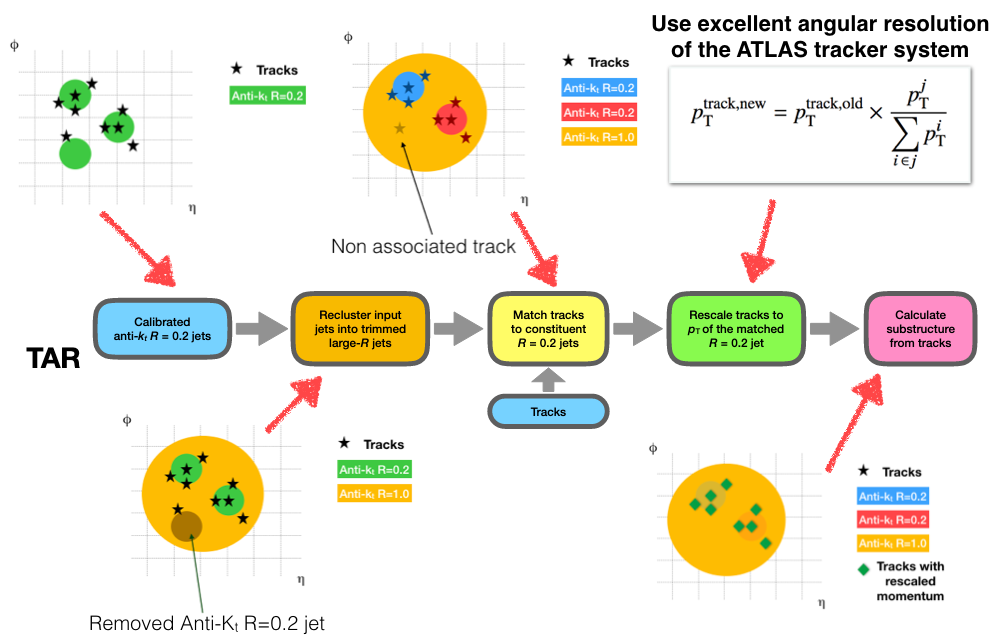
\includegraphics[width=0.9\textwidth]{Figures/3/TAR_alg.png}
    \caption{A visual summary of the TAR Jet algorithm.}
    \label{fig:TAR_alg}
\end{figure}

\subsection{Missing Transverse Momentum (\met)}
In the ATLAS detector, the beams collide directly along the longitudinal axis. As a result of the conservation of momentum, all decay products from the collision should thus have a total transverse momentum of 0. Using this information, missing transverse momentum (\met) can be used to represent undetected objects. In the signal model described in Section \ref{subsection:dh_model} both the neutrino from the leptonically decaying $W$-boson and the dark matter would not be directly detected in ATLAS. It is impossible to disentangle these objects, and they are reconstructed together using \met. \met is calculated for this analysis using baseline electrons and muons as described in subsections \ref{subsection:electrons} and \ref{subsection:muons}, as well as $R=0.4$ jets with the \verb|Tight| working point applied. No photons or \tau-leptons are included in the calculation. An additional soft term, which is calculated from tracks not associated with the reconstructed objects, is also added.

\subsubsection{\met Significance}
The significance of the \met measurement is also assessed using the object-based \met significance \metsig. It is calculated as described in \cite{MetSig} from a combination of the uncertainties on the reconstructed objects and soft term used to calculate \met, as well as a pileup correction. A high \metsig indicates a higher degree of confidence that the \met measurement of an event comes from an unseen object rather than from particle mismeasurement.

\section{Data and MC Preparation}
After reconstruction (or simulated reconstruction) in the ATLAS detector, data and MC events are stored as Analysis Object Data files which contain all reconstructed information from each event. Data and MC samples used for this analysis are initially in ATLAS Derived Analysis Object Data (DAOD format) which are created by skimming and slimming the AODs according to the EXOT27 job options. The DAODs include information about:
\begin{itemize}
	\item electrons, photons, muons, taujets,
	\item $R=1.0$ ``Large-R" jets,
	\item AntiKt4EMTopoJets, AntiKt4EMPFlowJets, AntiKt2LCTopoJets,
  \item Jet b-tagging, and
	\item InDetTrackParticles associated with AntiKt4EMTopoJets and AntiKt2LCTopoJets
\end{itemize}

The DAOD files are still too large to be convenient for analysis, and some analysis variables have not yet been calculated. In order to further process the DAODs we use the XAMPP analysis framework, which is built on top of the SUSYTools framework. We use a customized version of the XAMPP framework (XAMPPMonoSlep) maintained by the analysis team to calculate all necessary analysis variables and selects physics objects according to the definitions in Section \ref{section:objects}. We use the following set of ``preselection" criteria to trim the number of events to a convenient size prior to optimization, without cutting into any regions of sensitivity:
\begin{itemize}
\item passed \met trigger,
\item (1 signal muon or 1 signal electron) and no additional baseline muons or electrons,
\item \met > 150 \GeV,
\item \metsig > 5,
\item transverse mass of \met and lepton \mtlepmet > 50 \GeV,
\item veto on b-tagged $R=0.4$ jets, and
\item \(\NTAR > 0\) or \(\Njets > 1\).
\end{itemize}

The trigger requirements beyond the preselection criteria are discussed in further detail in Section \ref{section:trig}.  After processing by the XAMPPMonoSlep framework the data is stored in CERN Root files known as ntuples, which are further slimmed to include only necessary variables using XAMPPPlotting. At this stage the data and MC samples are ready to be analyzed.

	\startchapter{Analysis}
\label{chapter:analysis}

	\startchapter{Results}
In order to provide a comprehensive prediction of the sensitivity of the analysis regions to the signal model, we perform an exclusion fit. In an exclusion fit, the signal model plus the standard model background is taken as the null hypothesis and is tested against the alternative hypothesis of the background-only model. The following chapter describes the process of the fit, and provides the results.

\section{Statistical Framework}
\label{section:stats}
In each signal region, we create a histogram of all events in the sample that are within the region, consisting of several bins of a chosen variable $x$. The expectation value for the number of events in a single bin is:
\begin{equation}
E[n_i] = \mu s_i(\boldsymbol{\theta}) + b_i(\boldsymbol{\theta}),
\end{equation}
where $\mu$ is the parameter of interest, the signal strength, which is 0 in the background-only case and 1 in the nominal signal model. The vector of variables $\boldsymbol{\theta}$ represents the set of nuisance parameters, and $s_i$ and $b_i$ are the expected number of signal and background events in bin $i$:
\begin{equation}
\begin{gathered}
s_i = s_{tot} \int_{\text{bin i}} f_s(x|\boldsymbol{\theta}) dx \\
b_i = b_{tot} \int_{\text{bin i}} f_b(x|\boldsymbol{\theta}) dx.
\end{gathered}
\end{equation}
Here, $f_s(x|\boldsymbol{\theta})$ and $f_b(x|\boldsymbol{\theta})$ are the probability density functions of the variable $x$ for signal and background events. The variables $s_{tot}$ and $b_{tot}$ contain the total mean numbers of signal and background events, where $b_{tot}$ is allowed to vary and $s_{tot}$ is fixed to the value predicted by the MC signal samples.
In each control region, we build a similar histogram with a single bin with the expected value:
\begin{equation}
E[m_i] = b_i(\boldsymbol{\theta}).
\end{equation}
We can then construct a likelihood function from the product of Poisson probabilities for each bin:
\begin{equation}
L(\mu,\boldsymbol{\theta}) = C_{sys}(\boldsymbol{\theta}^0,\boldsymbol{\theta})\prod_{j=1}^{N} \frac{E[n_j]}{n_j!}e^{-E[n_j]} \prod_{k=1}^{M} \frac{E[m_k]}{m_k!}e^{-E[m_k]},
\end{equation}
where $C_{sys}(\boldsymbol{\theta}^0,\boldsymbol{\theta})$ is a product of probability distributions for the measurements describing each systematic uncertainty. These are taken to be Gaussian distributed, and are each scaled to have unit standard deviations, giving:
\begin{equation}
C_{sys}(\boldsymbol{\theta}^0,\boldsymbol{\theta}) = \prod_{m\in S} G(\boldsymbol{\theta}^{0}_{m} - \boldsymbol{\theta}_m, \sigma = 1).
\end{equation}
We then test a hypothesized value of the signal strength \mu~using the profile log-likelihood ratio as the test statistic:
\begin{equation}
\label{eq:prof_likelihood_ratio}
t_{\mu} = -2\log\Bigg( \frac{L(\mu_\text{sig}, \hat{\hat{\boldsymbol{\theta}}})}{L(\hat{\mu}_\text{sig}, \hat{\boldsymbol{\theta})}} \Bigg),
\end{equation}
where $\hat{\hat{\boldsymbol{\theta}}}$ is the set of nuisance parameters which maximize the likelihood function for the chosen signal strength $\mu_{\text{sig}}$, and $\hat{\boldsymbol{\theta}}$ and $\hat{\mu}_{\text{sig}}$ are the unconditional maximum-likelihood estimators for $L$. From this we compute the $p$-value corresponding to a given signal strength $\mu_{\text{sig}}$ by integrating the probability distribution of $t_{\mu}$:
\begin{equation}
p_{\mu} = \int_{t_{\mu_\text{obs}}}^\infty f(t_{\mu}|\mu_\text{sig}, \boldsymbol{\theta})dt_{\mu}.
\end{equation}
This probability distribution can be estimated by generating toy MC experiments, however in the ``asymptotic" regime with sufficiently high statistics (usually at least $\mathcal{O}(5)$ expected signal events) this distribution is known to follow a $\chi^2$ distribution according to Wilks theorem \cite{Wilks}.
Using this $p$-value formula, we follow the $\text{CL}_\text{s}$ technique to present results \cite{CLs}. We calculate $\text{CL}_\text{s+b}$ as the $p$-value for the existence of the signal model with some $\mu_{\text{sig}} > 0$ and $1 - \text{CL}_\text{b}$ as the $p$-value for the background-only case $\mu_{\text{sig}} = 0$:
\begin{equation}
\begin{gathered}
\text{CL}_\text{s+b}(\mu_\text{sig}) = \int_{t_{\mu_\text{obs}}}^\infty f(t_{\mu}|\mu_\text{sig}, \boldsymbol{\theta})dt_{\mu} \\
1 - \text{CL}_\text{b} = \int_{t_{\mu_\text{obs}}}^\infty f(t_{\mu}|0, \boldsymbol{\theta})dt_{\mu}.
\end{gathered}
\end{equation}
$\text{CL}_\text{s}$ is then given by the ratio of these two quantities:
\begin{equation}
\text{CL}_\text{s}(\mu_\text{sig}) = \frac{\text{CL}_\text{s+b}(\mu_\text{sig})}{1 - \text{CL}_\text{b}}.
\end{equation}

To perform an exclusion fit, we evaluate $\text{CL}_\text{s}$ for the nominal signal strength $\mu_{\text{sig}} = 1$, and exclude signal models with $\text{CL}_\text{s}(1) > 0.05$. We perform this statistical anlysis of the finalized analysis regions using the HistFitter software package \cite{HistFitter}.

\section{Minimum \ms}
As a discrimination variable for the exclusion fit, we use a partial reconstruction of the $s$ mass. The $s$ can not be fully reconstructed because the \met derived from the neutrino cannot be distinguished from the \met derived from dark matter. Instead, we calculate the minimum possible $s$ mass \minms consistent with the other measured $s$ decay products. This variable shows good discrimination power, but is not used in the signal region selection because the distribution shape varies widely across signal points according to their $s$ mass.

To calculate \minms, we begin by using the $W$ mass constraint on the charged lepton-neutrino system to solve for the neutrino energy $E_{\nu}$ as a function of the angle $\theta_{\ell\nu}$ between the charged lepton and neutrino:
\begin{equation}
\begin{gathered}
    \label{eqn:Ev}
		E_{\nu} = \frac{m_W^2}{2E_l(1 - \cos\ \theta_{l\nu})},\;{\rm where}\\
		m_W^2 = (p_l + p_{\nu})^2 = 2p_lp_{\nu} = 2E_lE_{\nu}(1 - \cos\ \theta_{l\nu}).
	\end{gathered}
\end{equation}
We then rotate the coordinate system to place the neutrino 3-momentum along the $z$-axis and the hadronic $W$ ($W_H$) 3-momentum in the $x$-$z$ plane. The neutrino 4-momentum is then:
\begin{equation}
	p_{\nu} = \frac{m_W^2}{2E_l(1 - \cos\ \theta_{l\nu})}(\sin \theta_{l\nu}, \sin \theta_{l\nu}\sin \phi_{\nu}, \cos \theta_{l\nu}, 1).
\end{equation}
We can then write the $s$ mass as:
\begin{multline}
\label{eqn:m_s}
	\begin{gathered}
		m_s^2 = (p_{W_H} + p_l + p_{\nu})^2\\
		m_s^2 = (E_{W_H} + E_l + E_{\nu})^2 - (p_{W_{Hx}} + E_{\nu}\sin \theta_{l\nu}\cos \phi_{\nu})^2 - (E_{\nu}\sin \theta_{l\nu}\sin \phi_{\nu})^2 \\- (E_l + p_{W_{Hz}} + E_{\nu}\cos \theta_{l\nu})^2.
	\end{gathered}
\end{multline}
It is clear from this equation that $m_s$ is minimized with $\phi_{\nu} = 0$, and substituting this and Equation \ref{eqn:Ev} for $E_v$ we are left with an expression for $m_s$ with $\theta_{l\nu}$ as the only remaining unknown variable:
\begin{multline}
m_s^2 = \left(E_l + \frac{m_W^2}{2E_l(1 - \cos\ \theta_{l\nu})} + E_{W_H}\right)^2 - \left(|\vec{p_{W_H}}|\sin \theta_{W_l} + \frac{\sqrt{1 - \cos^2 \theta_{l\nu}}m_W^2}{2E_l(1 - \cos\ \theta_{l\nu})}\right)^2 \\- \left(E_l + |\vec{p_{W_H}}|cos \theta_{W_l} + \frac{\cos \theta_{l\nu}m_W^2}{2E_l(1 - \cos\ \theta_{l\nu})}\right)^2.
\end{multline}
We then vary $\theta_{l\nu}$ on the interval $[0,\pi]$ to search for the minimum $m_s$.
Figure \ref{fig:ms} shows the signal and background distributions of \minms in both signal regions, demonstrating the strong discrimination potential and large variance between signal samples that make it an ideal model fitting variable. During model fitting we place events in 5 equal-width bins in the range $125 \leq \ms \leq 375$ GeV.

\begin{figure}[htbp]
  \centering

     \begin{subfigure}{0.49\textwidth}
     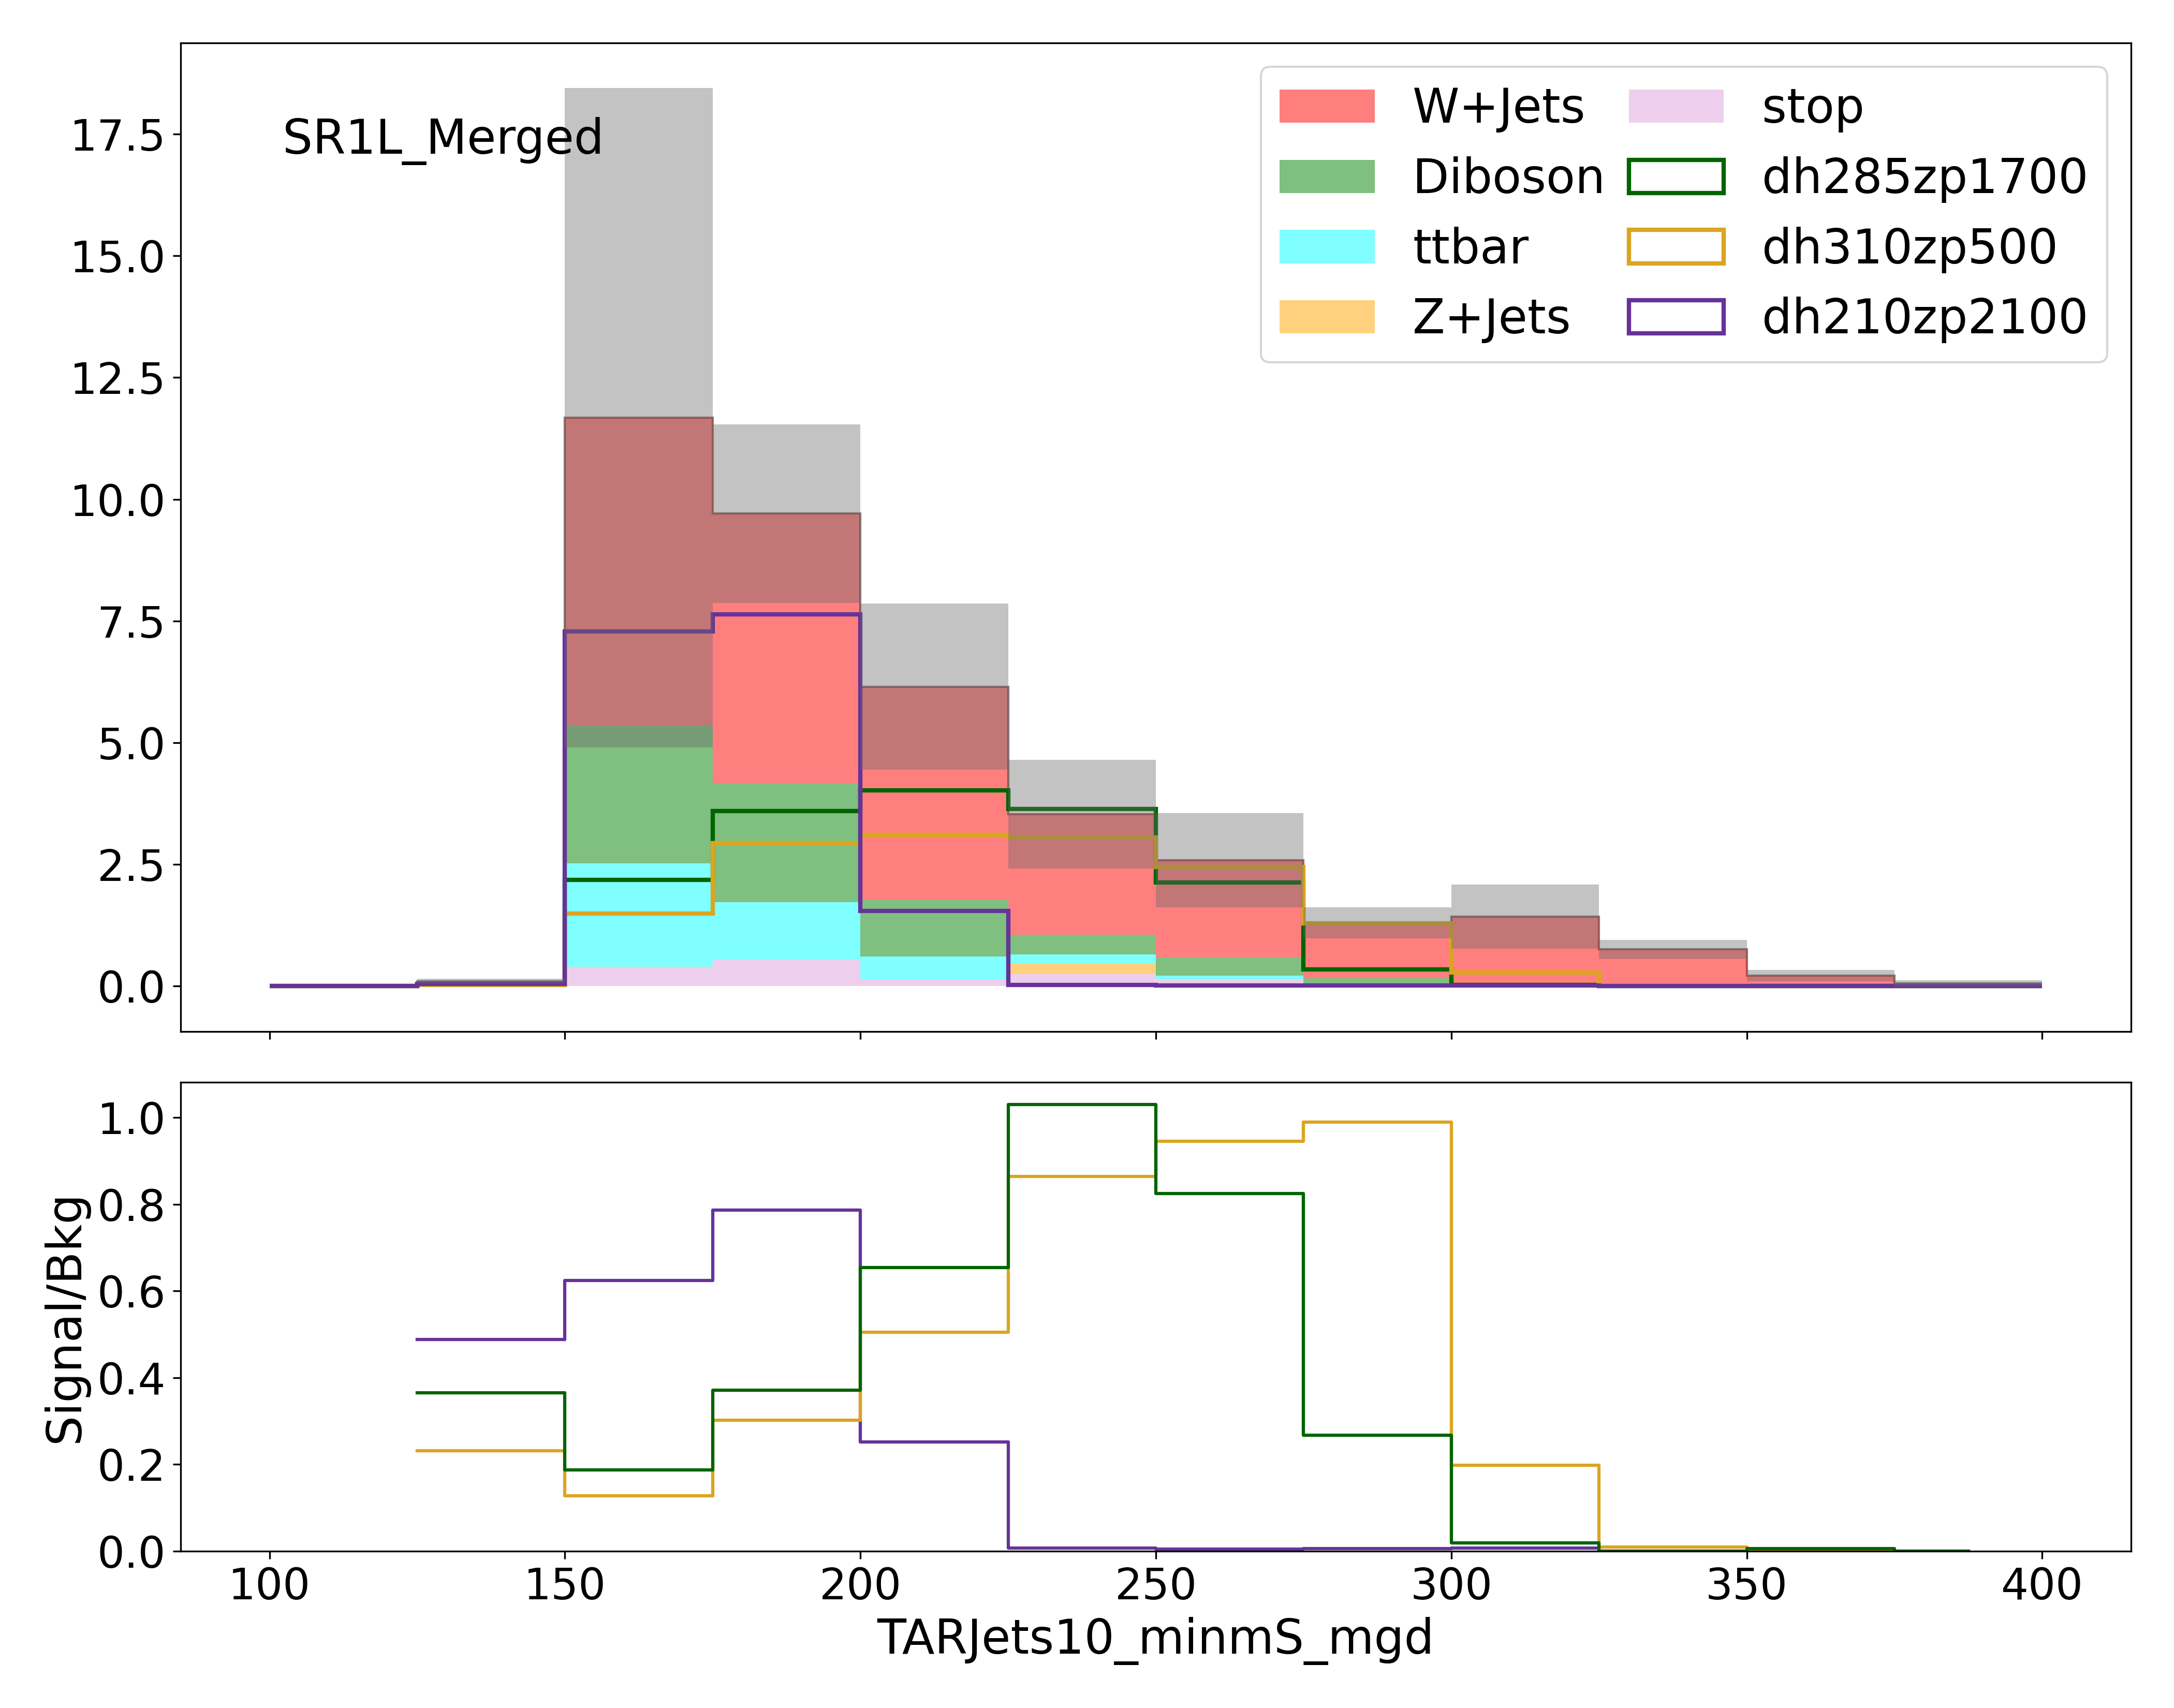
\includegraphics[width = 0.98\textwidth]{Figures/5/ms/SR1L_Merged/TARJets10_minmS_mgd.png}
     \caption{``Merged" SR}
     \end{subfigure}
     \begin{subfigure}{0.49\textwidth}
     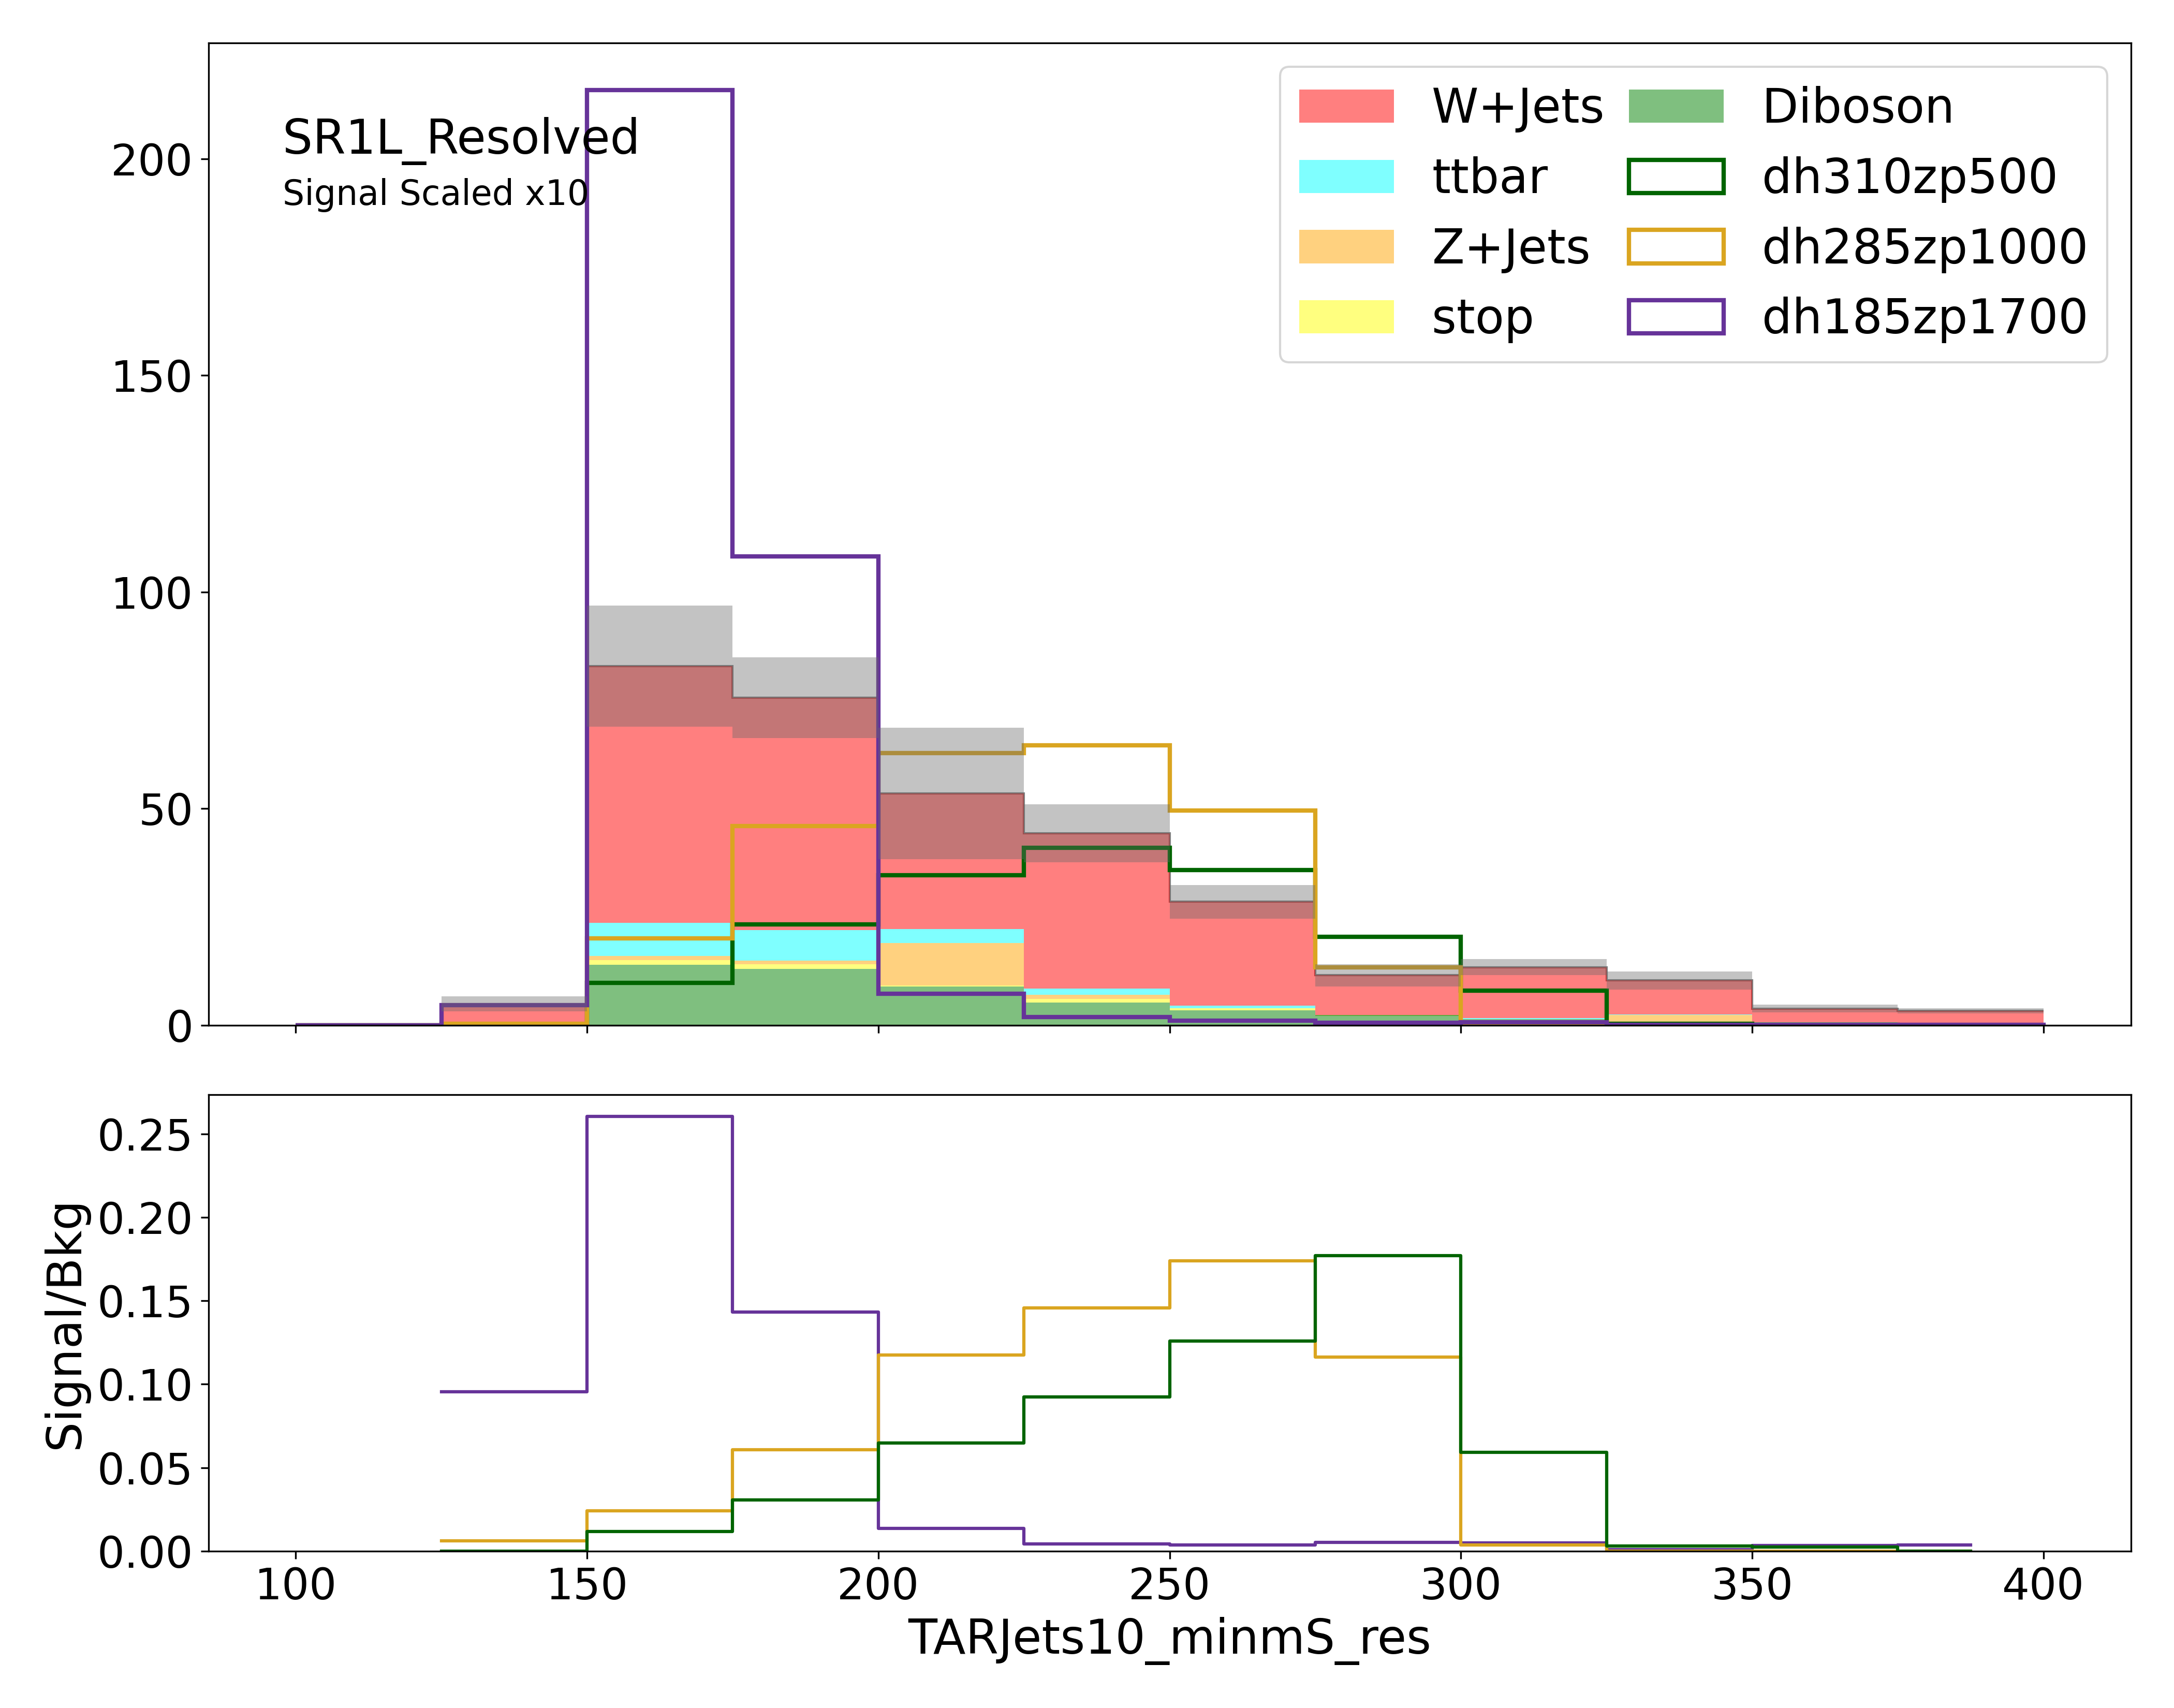
\includegraphics[width = 0.98\textwidth]{Figures/5/ms/SR1L_Resolved/TARJets10_minmS_res.png}
     \caption{``Resolved" SR}
     \end{subfigure}

     \caption{Distributions of \minms in the \merged and \resolved signal regions.}
     \label{fig:ms}
  \end{figure}
\FloatBarrier
\section{Systematic Uncertainties}
Statistical fluctuations are uncorrelated between measurements that use non-overlapping datasets, and arise from a measurement consisting of a limited number of observations. Systematic uncertainties, however, are often correlated in measurements that do not necessarily use overlapping datasets, generally do not scale with the sample size, and may derive from the nature of the experiment or uncertainty in the model used to make conclusions about the data.  For this analysis, we further categorize systematic uncertainties into theory uncertainties on the modelling and experimental uncertainties. The evaluation of theory uncertainties is not within the scope of this thesis, and I assign them a flat value of 20\% of the yield on each background category. I chose a value of 20\% based on the magnitude of the SM modelling uncertainties observed in the fully-hadronic channel in \cite{had_analy} as well as ongoing work internal to the analysis. What follows is a short description of the various types of experimental systematic uncertainties that we consider in this thesis.

\subsection{$R=0.4$ Jets}
Uncertainties on $R=0.4$ jets are divided into jet energy scale (JES) and jet energy resolution (JER) uncertainties. These include, but are not limited to, uncertainties on pileup, flavour composition, and punch-through of jets.

\subsection{Track Uncertainties}
These are uncertainties on the reconstruction of tracks in the ATLAS inner detector. In this analysis they are primarily propagated into the reconstruction of TAR jets in the ``merged" signal and control regions.

\subsection{Muon and Electron}
For muons and electrons, we consider uncertainties on the reconstruction efficiency, isolation and identification, and energy or momentum scale and resolution.

\subsection{\met}
We propagate uncertainties on the aformentioned objects into the \met calculation, however we consider separate \met systematics which affect the reconstruction of the \met soft term.

\subsection{Luminosity}
The integrated luminosity measured across the run-2 data taking period is known to a precision of 1.7\% \cite{lumi_unc}. This is therefore applied as an overall systematic across the normalization of all MC events.

\section{Fit Results}
\subsection{Background Only Fit}
I first perform a background-only fit to examine the effects of systematic uncertainties and control region normalization on background predictions in the signal regions. The signal regions for this analysis remain blinded; therefore ATLAS data in the signal regions is mimicked by Asimov data with a yield equal to the nearest integer value to the pre-fit total background yield in each bin.

Figures \ref{fig:bkg_only_mgd} and \ref{fig:bkg_only_res} show comparisons of the pre-fit and post-fit yields in each region for the background only fit, while Tables \ref{tab:yields_mgd} and \ref{tab:yields_res} give a more detailed numerical breakdown. In the \merged signal region, the fit increases the expected number of SM events primarily due to an increase in expected \wjets events from the normalization derived in the \merged \wjets control region. In the \resolved signal region, the fit decreases the expected background yield, again primarily due to normalization this time from the \resolved \wjets control region. In both cases the uncertainty on the predicted \wjets yield is reduced. In both the \merged and \resolved categories the \ttbar control regions slightly reduce the predicted \ttbar yield and substantially reduce the uncertainty on those predictions.

Tables \ref{tab:systs_mgd} and \ref{tab:systs_res} summarize the uncertainty on the total yield in each analysis region from statistical and systematic sources. Uncertainties preceded by ``\mu", ``\alpha", and ``\gamma" represent normalization, systematic, and statistical uncertainties respectively. The leading sources of uncertainty in both signal regions are normalization factors and theory uncertainties on the \wjets background, followed by a mix of JER experimental systematics and bin-by-bin statistical uncertainties.

\begin{table}[t]
\centering
\small
%%
\begin{tabular*}{\textwidth}{@{\extracolsep{\fill}}lrrr}
\toprule
\textbf{table.results.yields channel}           & SR\_Merged            & CRW\_Merged            & CRTT\_Merged              \\
\midrule
%%
Observed events          & $49$              & $205$              & $59$                    \\
\midrule
%%
Fitted bkg events         & $46.88 \pm 8.87$          & $204.97 \pm 14.27$          & $58.93 \pm 7.66$              \\
\midrule
%%
        Fitted Diboson events         & $7.06 \pm 1.67$          & $27.65 \pm 6.53$          & $0.09 \pm 0.03$              \\
%%
        Fitted WJets events         & $34.09 \pm 8.15$          & $153.16 \pm 16.96$          & $0.37_{-0.37}^{+7.97}$              \\
%%
        Fitted ttbar events         & $2.85 \pm 0.76$          & $6.64 \pm 1.90$          & $52.30 \pm 11.30$              \\
%%
        Fitted ZJets events         & $0.33 \pm 0.10$          & $12.70 \pm 2.99$          & $0.00 \pm 0.00$              \\
%%
        Fitted stop events         & $1.32 \pm 0.36$          & $3.03 \pm 0.86$          & $6.17 \pm 1.35$              \\
%%
        Fitted Triboson events         & $1.22 \pm 0.15$          & $1.79 \pm 0.24$          & $0.01 \pm 0.00$              \\
%%
 \midrule
%%
MC exp. SM events              & $49.48 \pm 10.01$          & $214.54 \pm 43.34$          & $78.57 \pm 17.01$              \\
\midrule
%%
        MC exp. Diboson events         & $7.07 \pm 1.68$          & $27.70 \pm 6.58$          & $0.09 \pm 0.03$              \\
%%
        MC exp. WJets events         & $35.62 \pm 8.98$          & $160.16 \pm 38.82$          & $0.41_{-0.41}^{+8.31}$              \\
%%
        MC exp. ttbar events         & $3.92 \pm 1.01$          & $9.15 \pm 2.34$          & $71.90 \pm 14.59$              \\
%%
        MC exp. ZJets events         & $0.33 \pm 0.10$          & $12.72 \pm 3.01$          & $0.00 \pm 0.00$              \\
%%
        MC exp. stop events         & $1.32 \pm 0.36$          & $3.03 \pm 0.87$          & $6.17 \pm 1.36$              \\
%%
        MC exp. Triboson events         & $1.22 \pm 0.15$          & $1.79 \pm 0.24$          & $0.01 \pm 0.00$              \\
%%     \\
\bottomrule
\end{tabular*}
\caption{Pre and post-fit yields for each background category in the merged signal and control regions for a background-only fit.}
\label{tab:yields_mgd}
\end{table}

\begin{table}
\centering
\small
%%
\begin{tabular*}{\textwidth}{@{\extracolsep{\fill}}lrrr}
\toprule
\textbf{table.results.yields channel}           & SR\_Resolved            & CRW\_Resolved            & CRTT\_Resolved              \\
\midrule
%%
Observed events          & $309$              & $717$              & $87$                    \\
\midrule
%%
Fitted bkg events         & $314.82 \pm 35.79$          & $717.05 \pm 26.75$          & $87.06 \pm 9.30$              \\
\midrule
%%
        Fitted Diboson events         & $48.96 \pm 10.77$          & $105.34 \pm 21.98$          & $0.62 \pm 0.17$              \\
%%
        Fitted WJets events         & $231.59 \pm 32.86$          & $564.13 \pm 36.72$          & $4.40_{-4.40}^{+5.81}$              \\
%%
        Fitted ttbar events         & $24.00 \pm 5.26$          & $22.30 \pm 4.48$          & $72.74 \pm 11.22$              \\
%%
        Fitted ZJets events         & $3.51 \pm 1.05$          & $15.56 \pm 6.60$          & $0.00 \pm 0.00$              \\
%%
        Fitted stop events         & $4.12 \pm 1.13$          & $3.90 \pm 1.10$          & $9.28 \pm 2.22$              \\
%%
        Fitted Triboson events         & $2.64 \pm 0.26$          & $5.82 \pm 0.34$          & $0.01_{-0.01}^{+0.01}$              \\
%%
 \midrule
%%
MC exp. SM events              & $309.37 \pm 55.91$          & $707.82 \pm 120.45$          & $79.10 \pm 15.25$              \\
\midrule
%%
        MC exp. Diboson events         & $49.00 \pm 10.83$          & $105.43 \pm 22.13$          & $0.62 \pm 0.17$              \\
%%
        MC exp. WJets events         & $228.71 \pm 52.14$          & $557.21 \pm 115.70$          & $4.36_{-4.36}^{+5.85}$              \\
%%
        MC exp. ttbar events         & $21.40 \pm 5.09$          & $19.89 \pm 4.34$          & $64.83 \pm 13.64$              \\
%%
        MC exp. ZJets events         & $3.51 \pm 1.05$          & $15.58 \pm 6.61$          & $0.00 \pm 0.00$              \\
%%
        MC exp. stop events         & $4.12 \pm 1.13$          & $3.90 \pm 1.11$          & $9.28 \pm 2.23$              \\
%%
        MC exp. Triboson events         & $2.64 \pm 0.26$          & $5.82 \pm 0.34$          & $0.01_{-0.01}^{+0.01}$              \\
%%
%%     \\
\bottomrule
\end{tabular*}
\caption{Pre and post-fit yields for each background category in the resolved signal and control regions for a background-only fit.}
\label{tab:yields_res}
\end{table}

\begin{figure}[h]
  \centering

     \begin{subfigure}{0.49\textwidth}
     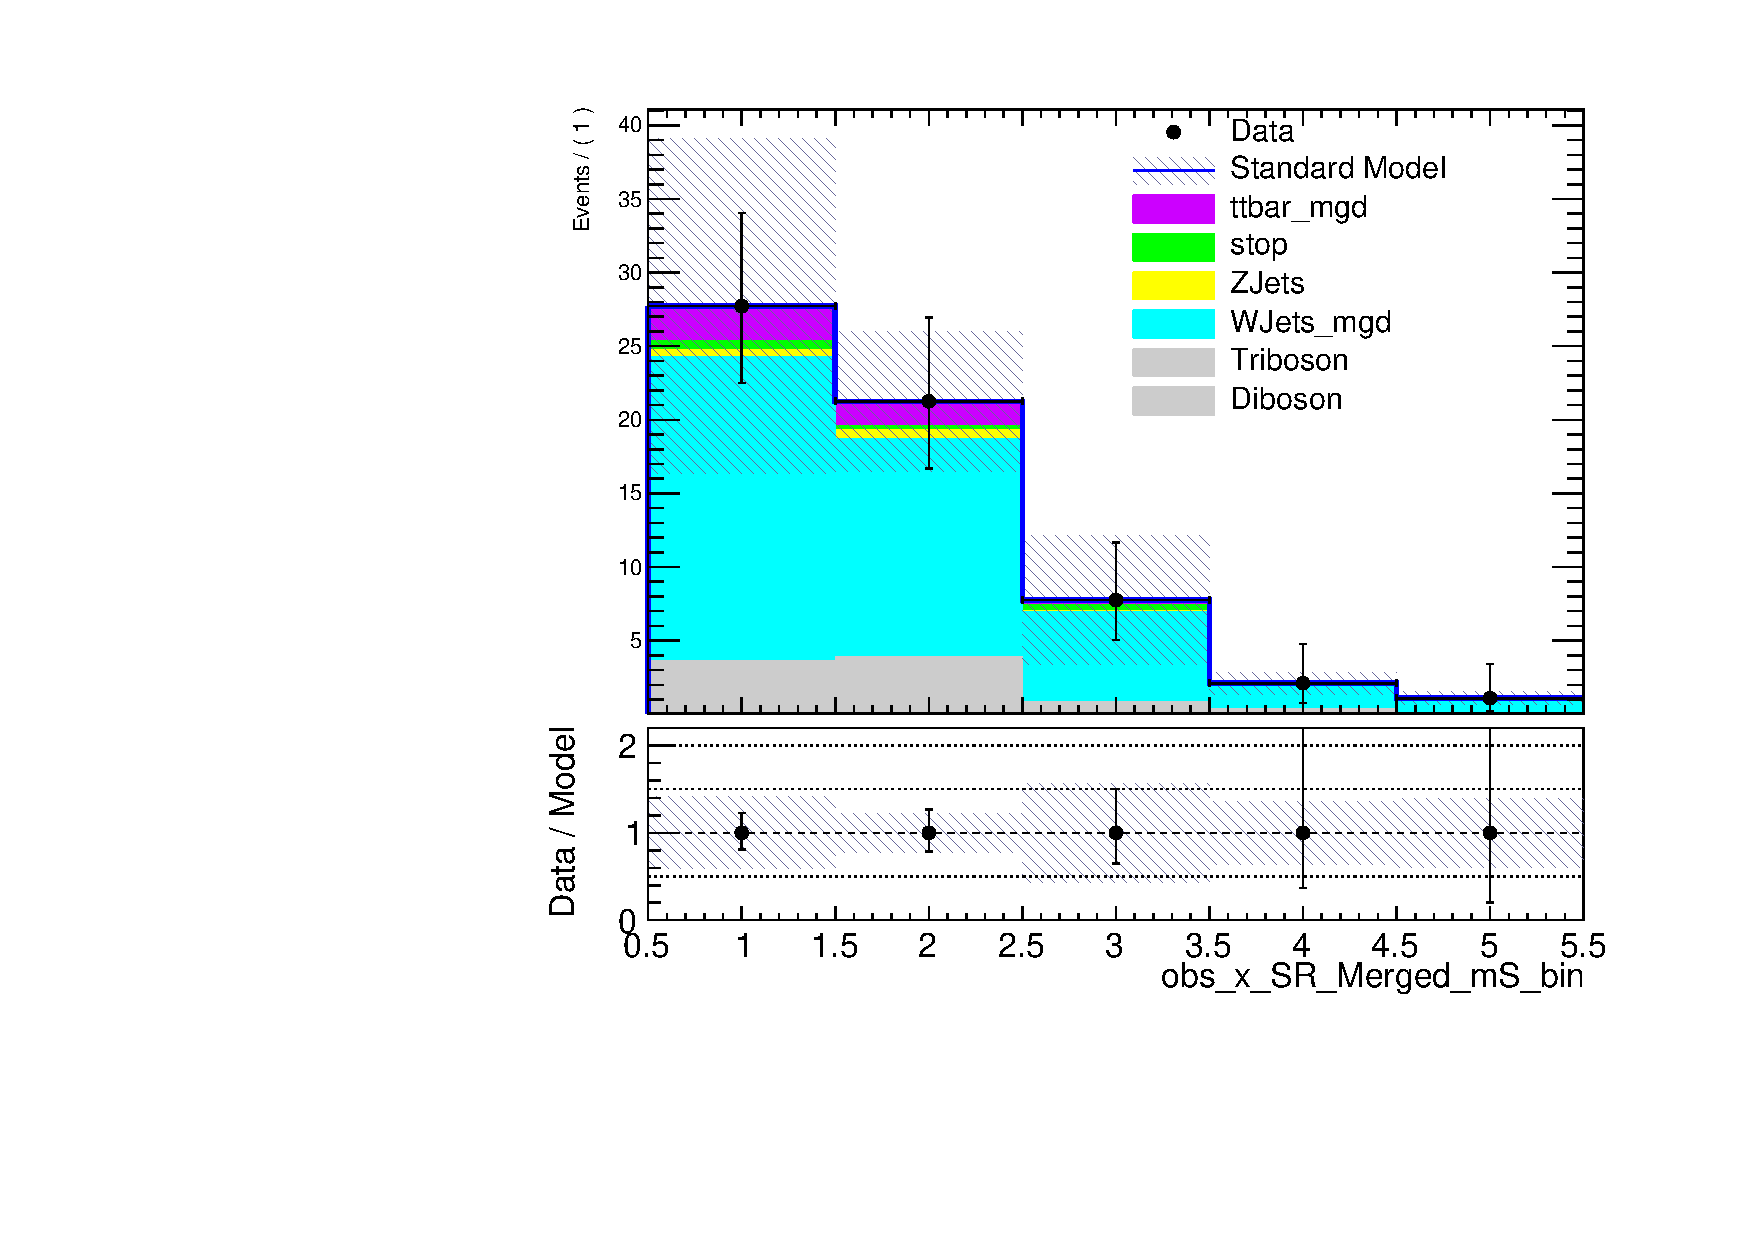
\includegraphics[width = 0.98\textwidth]{Figures/5/bkg_only/SR_Merged_mS_bin_beforeFit.pdf}
     \caption{Merged SR pre-fit}
     \end{subfigure}
     \begin{subfigure}{0.49\textwidth}
     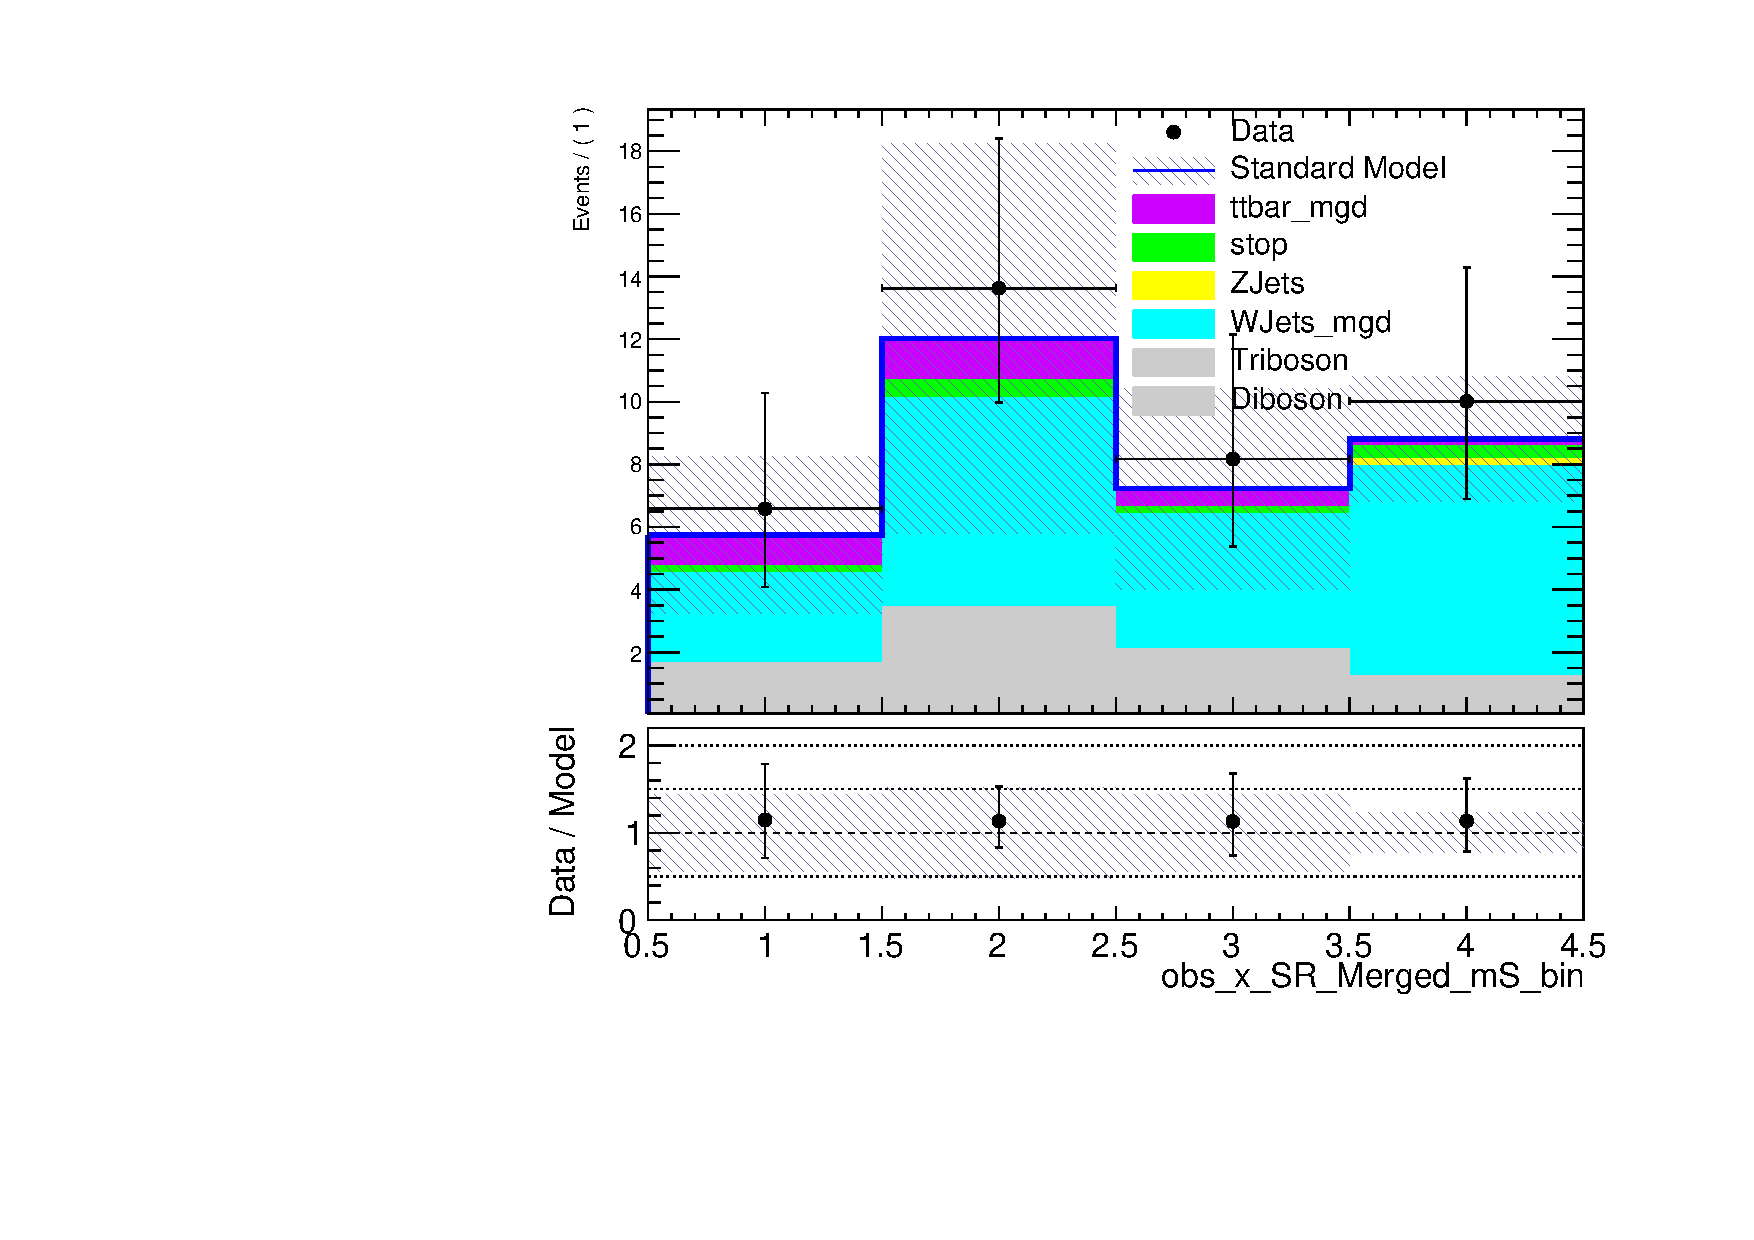
\includegraphics[width = 0.98\textwidth]{Figures/5/bkg_only/SR_Merged_mS_bin_afterFit.pdf}
     \caption{Merged SR post-fit}
     \end{subfigure}
     \begin{subfigure}{0.49\textwidth}
     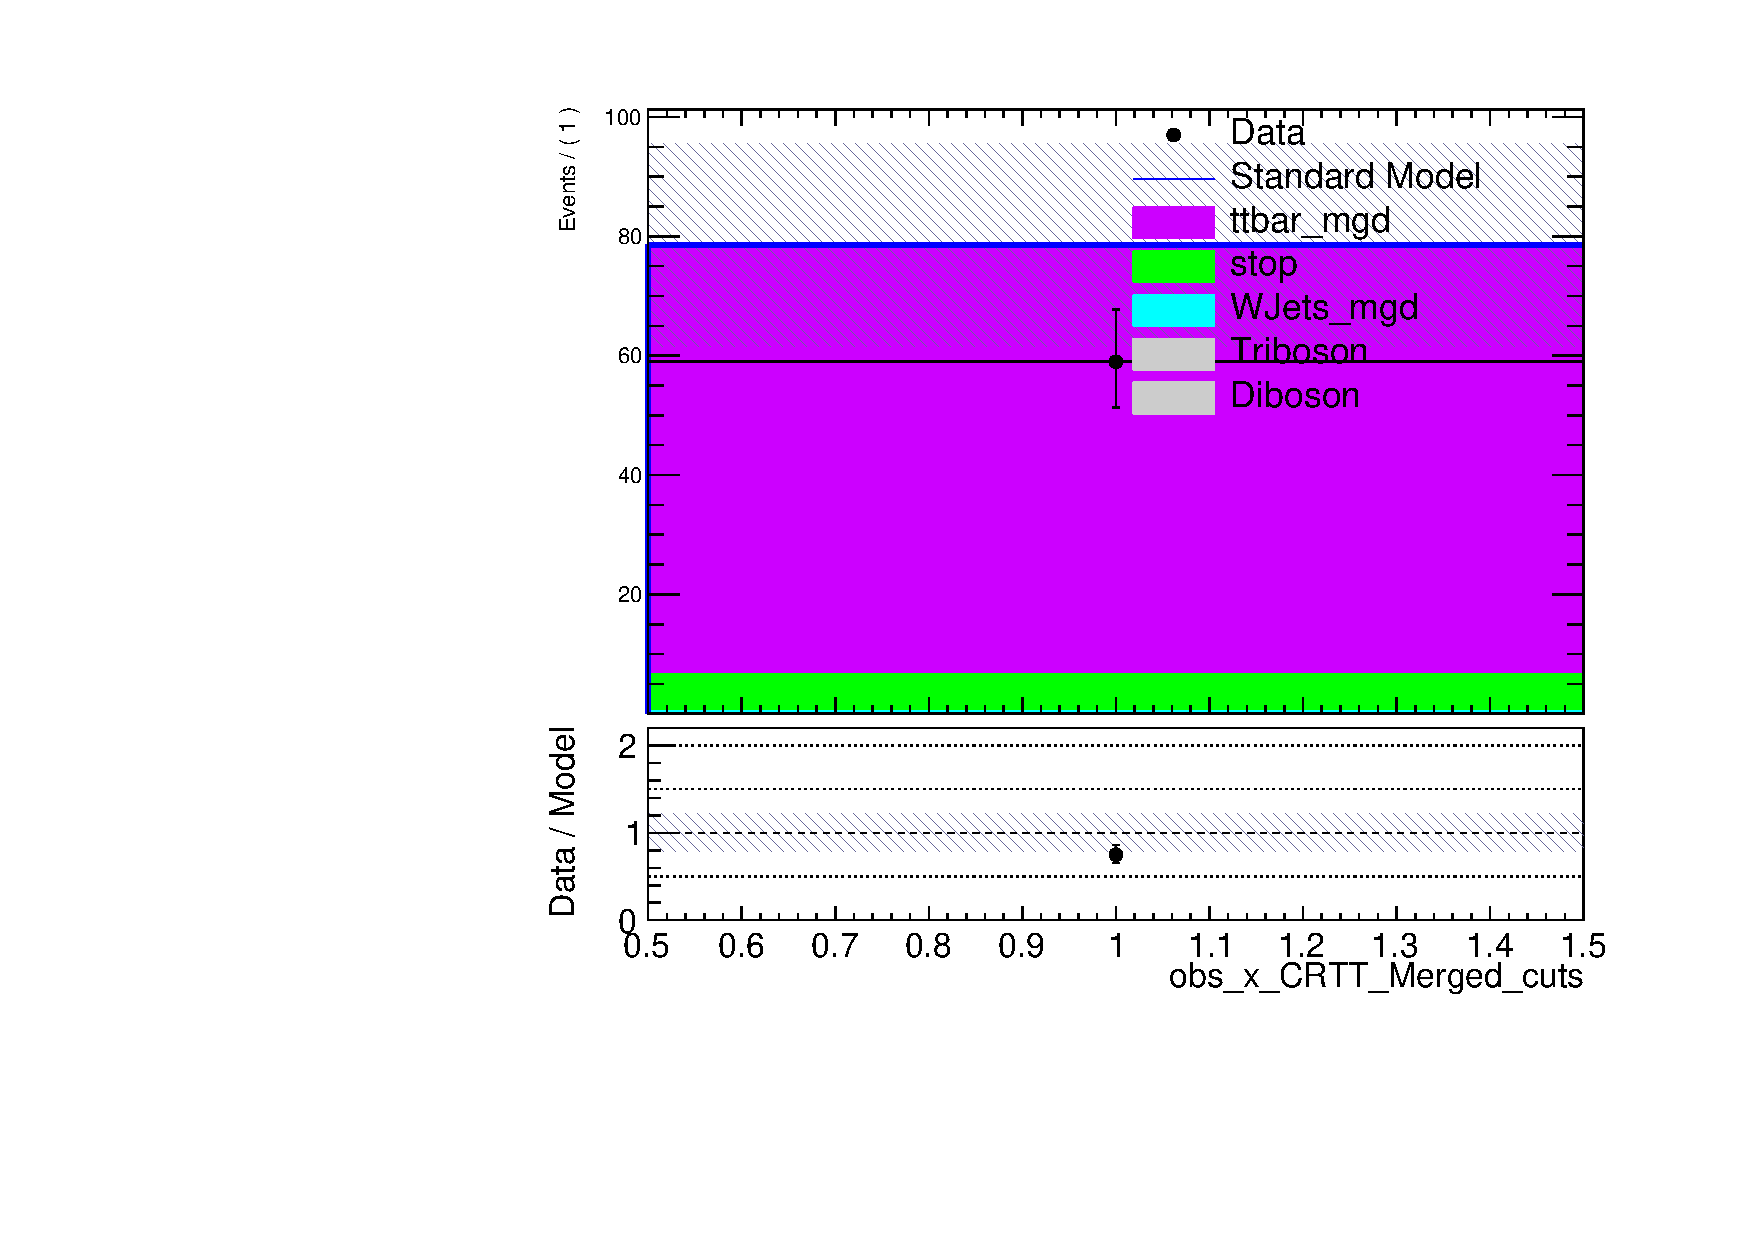
\includegraphics[width = 0.98\textwidth]{Figures/5/bkg_only/CRTT_Merged_cuts_beforeFit.pdf}
     \caption{Merged CR \ttbar pre-fit}
     \end{subfigure}
     \begin{subfigure}{0.49\textwidth}
     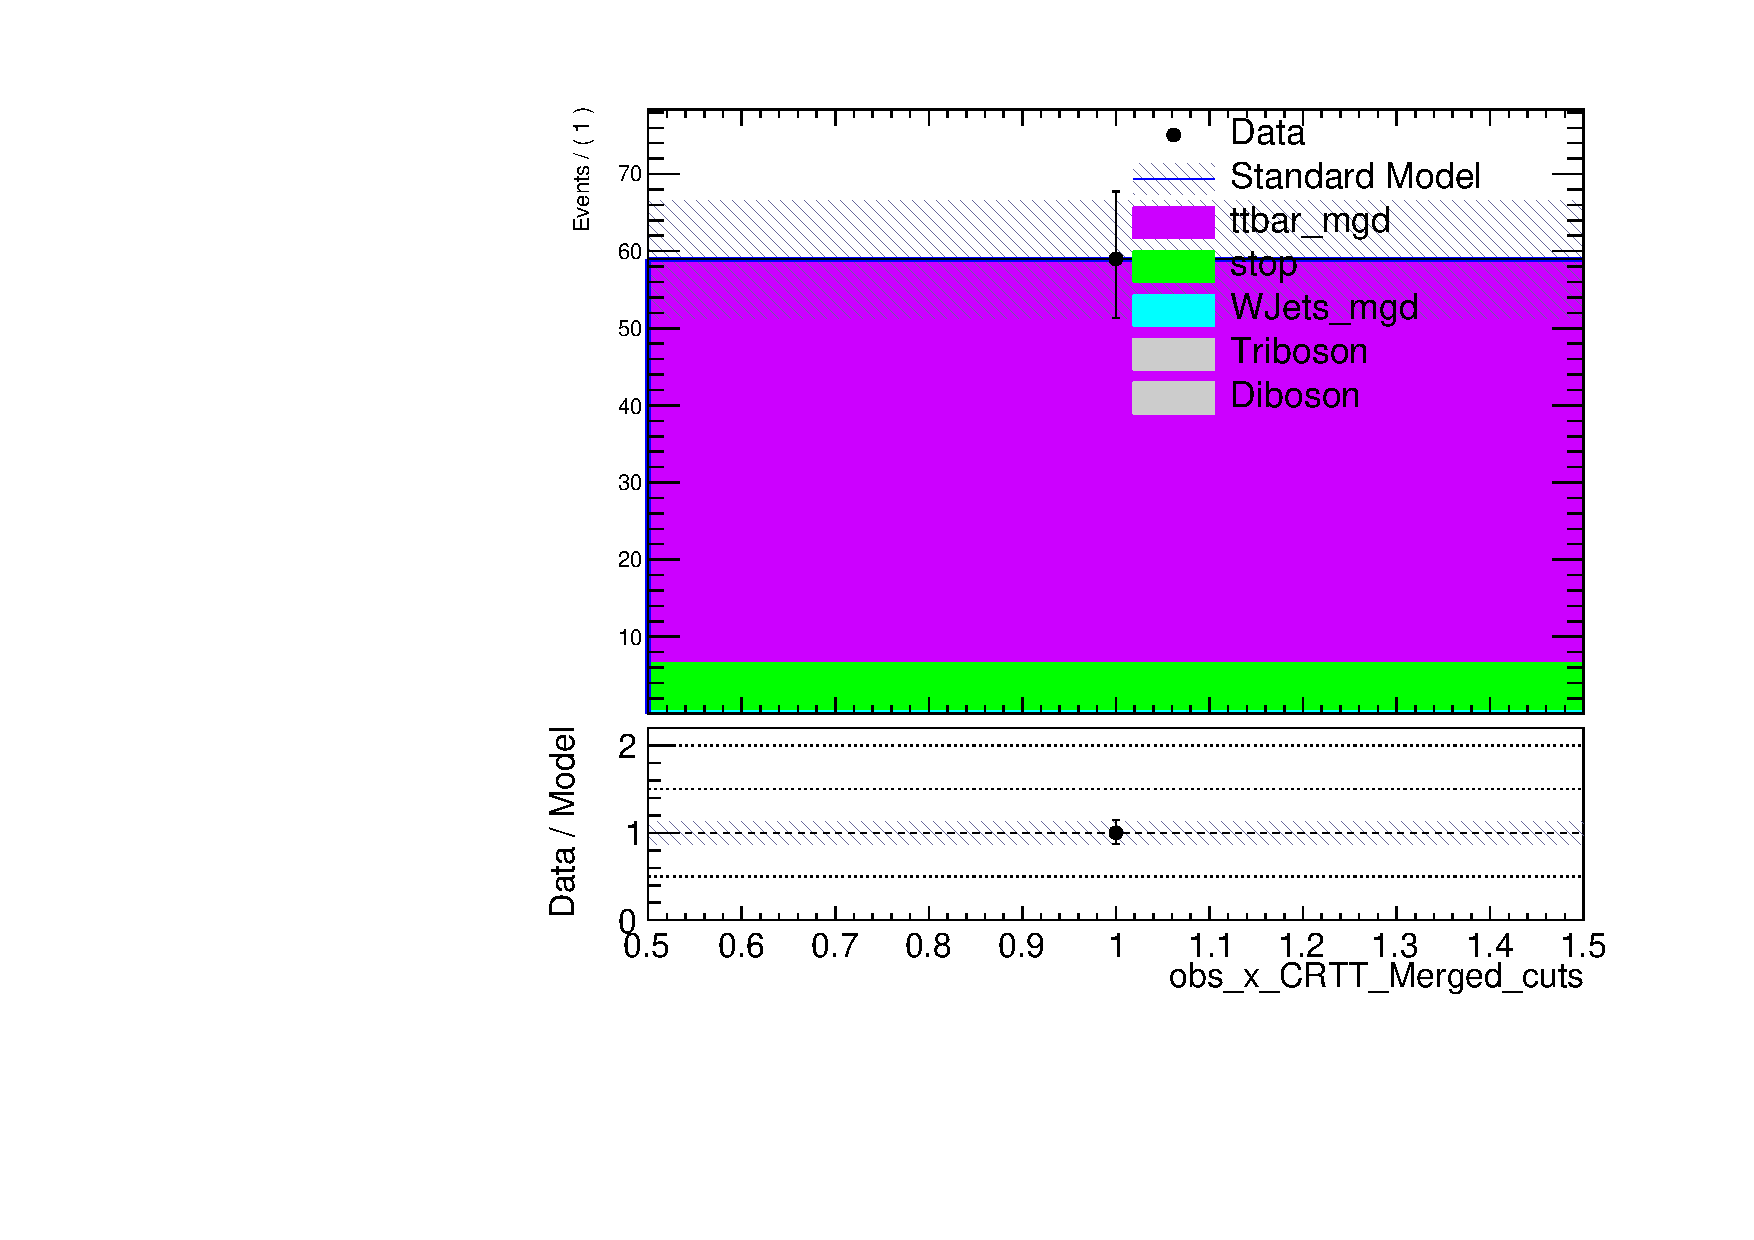
\includegraphics[width = 0.98\textwidth]{Figures/5/bkg_only/CRTT_Merged_cuts_afterFit.pdf}
     \caption{Merged CR \ttbar post-fit}
     \end{subfigure}
     \begin{subfigure}{0.49\textwidth}
     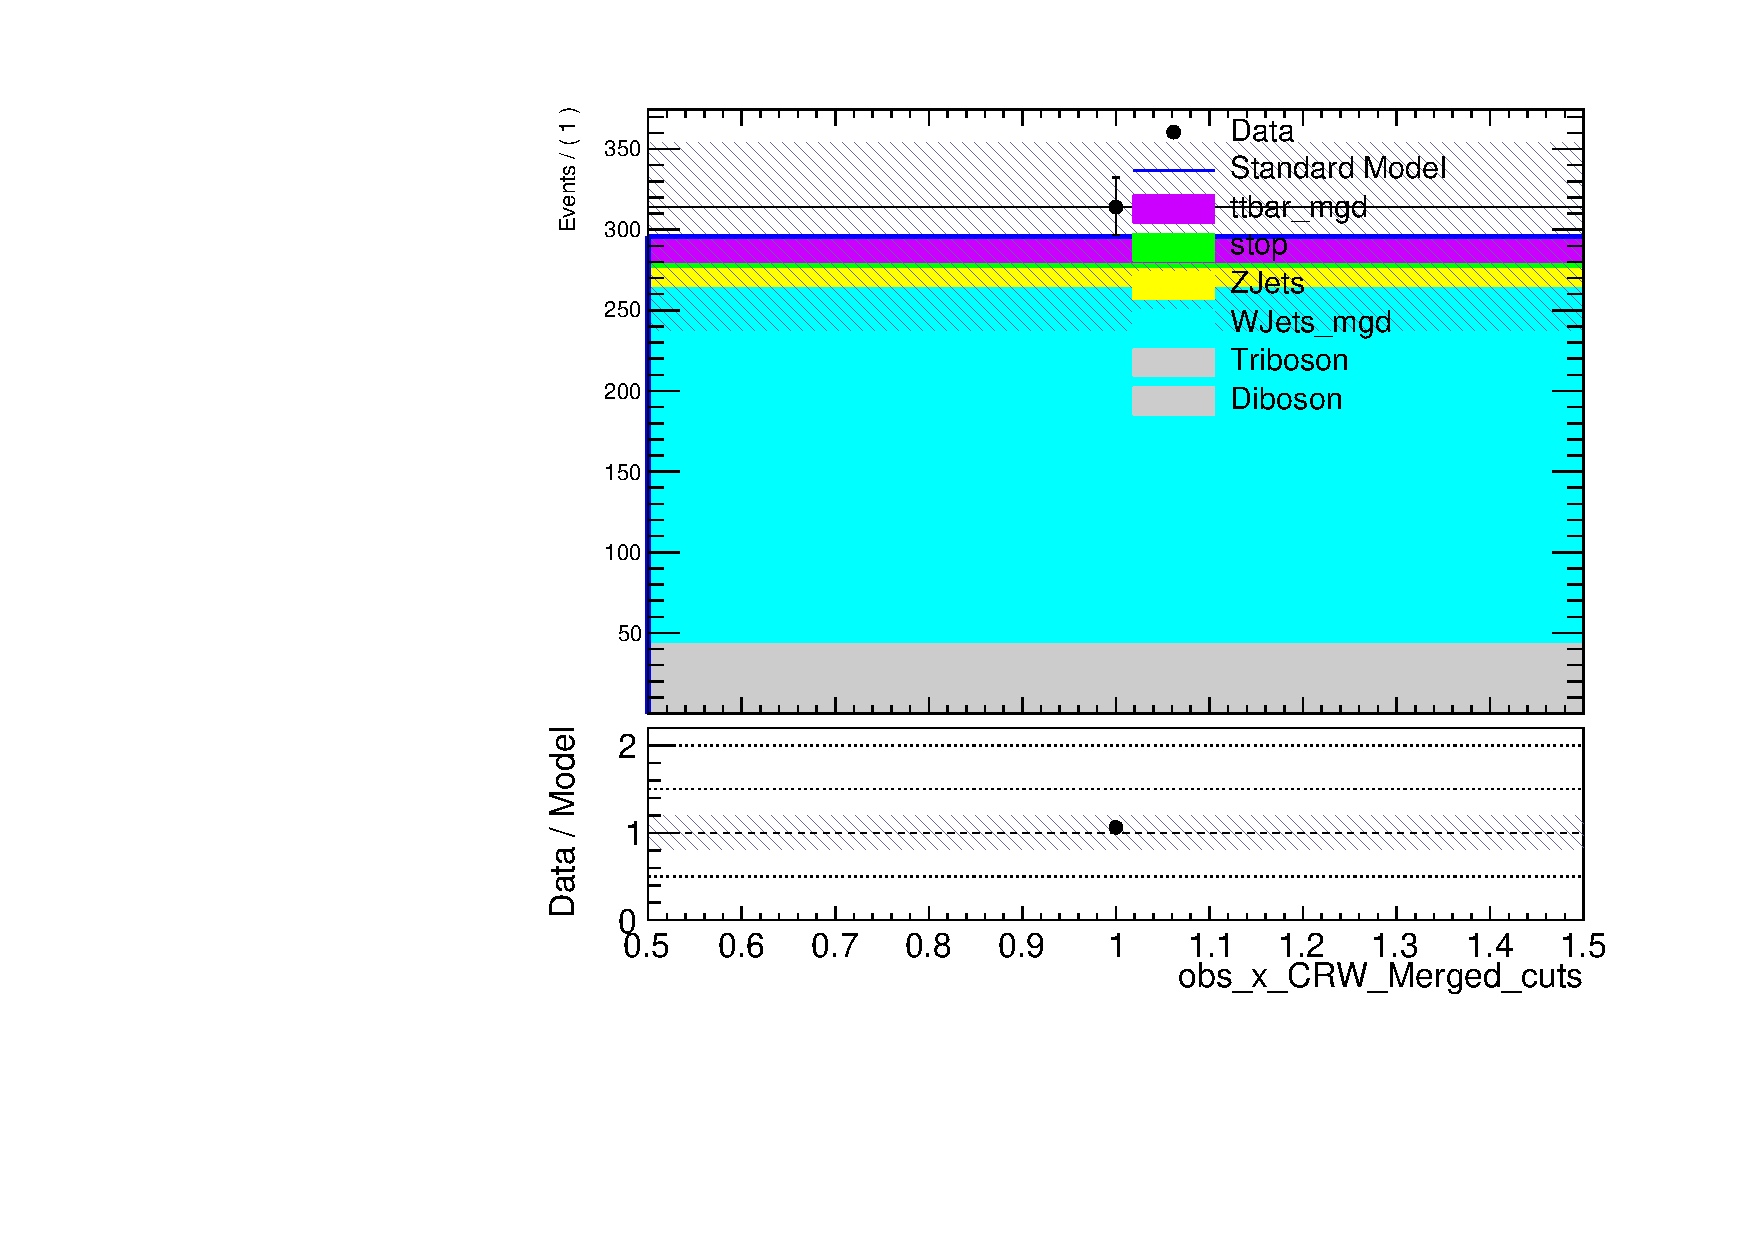
\includegraphics[width = 0.98\textwidth]{Figures/5/bkg_only/CRW_Merged_cuts_beforeFit.pdf}
     \caption{Merged CR \wjets pre-fit}
     \end{subfigure}
     \begin{subfigure}{0.49\textwidth}
     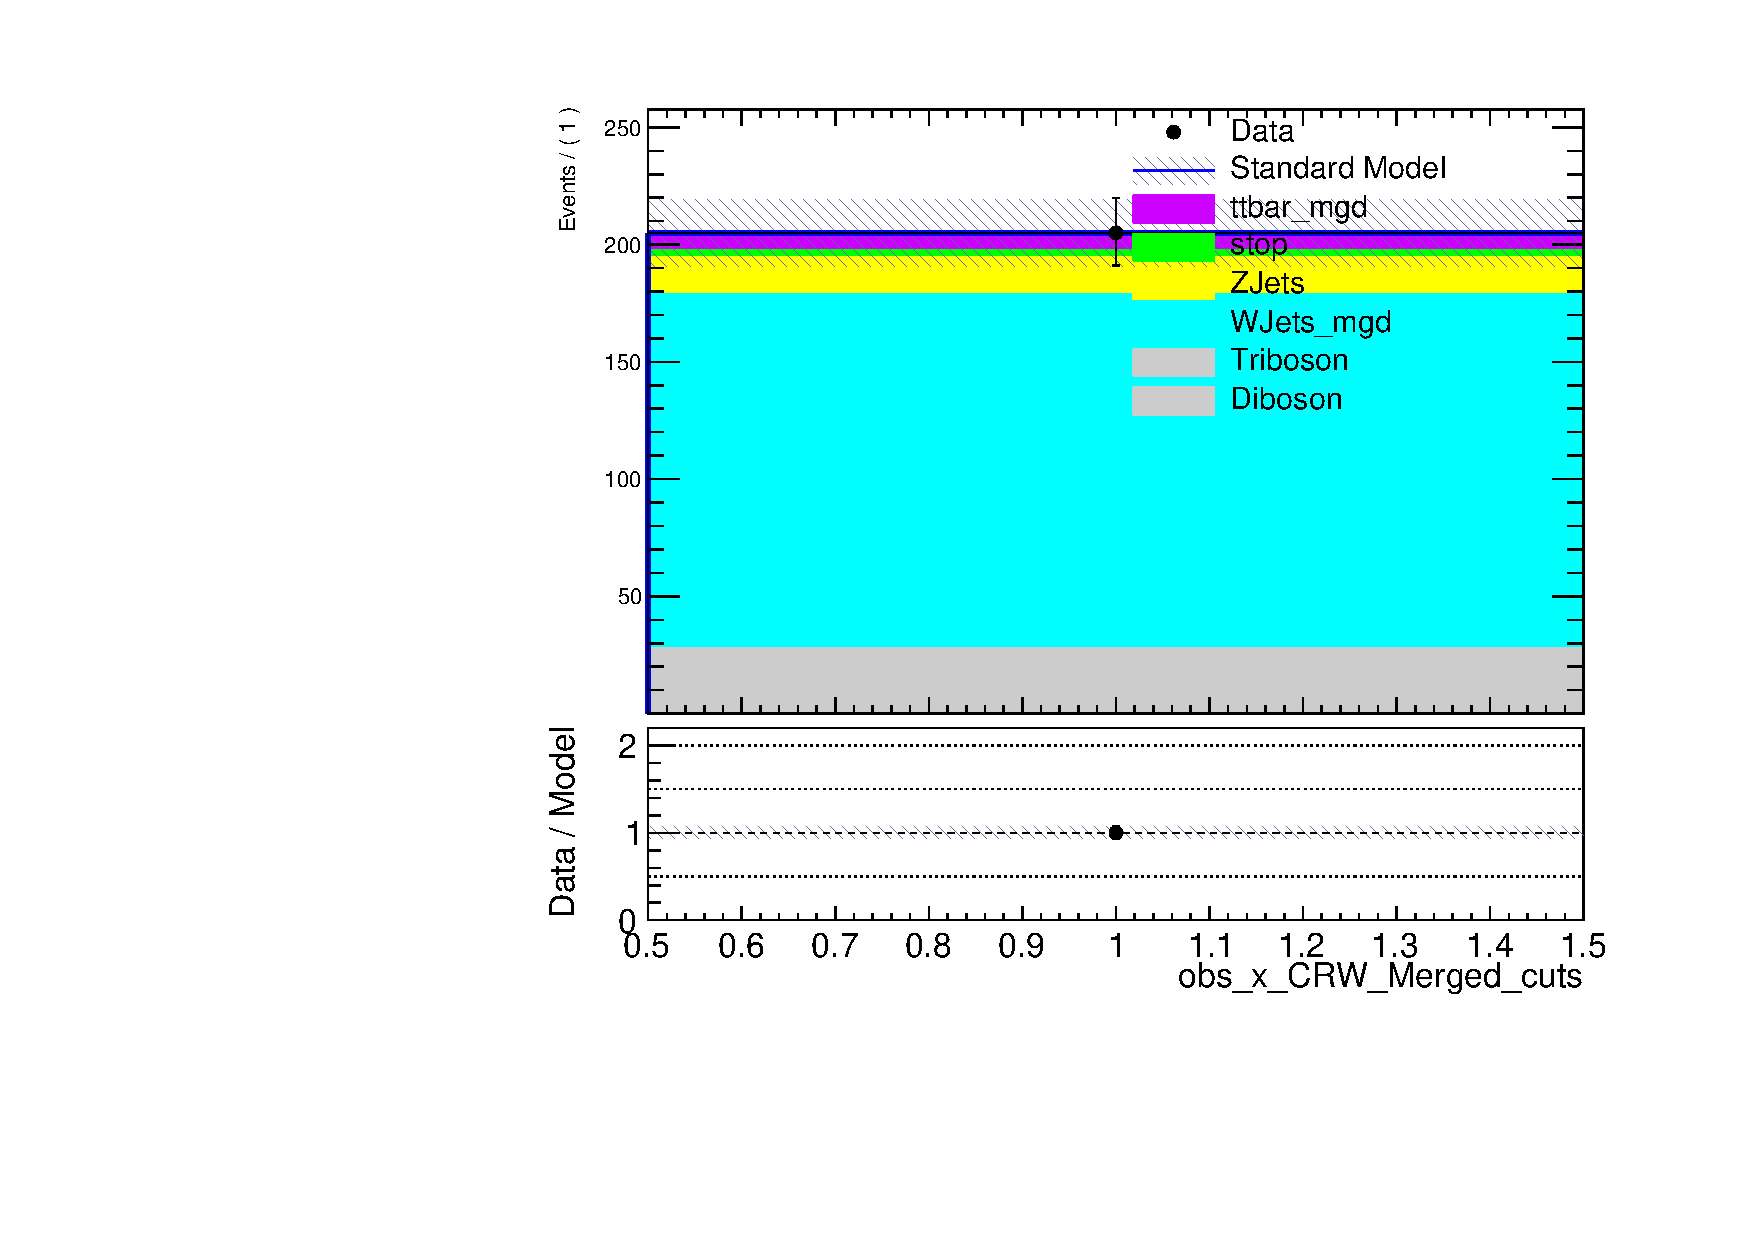
\includegraphics[width = 0.98\textwidth]{Figures/5/bkg_only/CRW_Merged_cuts_afterFit.pdf}
     \caption{Merged CR \wjets post-fit}
     \end{subfigure}

     \caption{Pre and post-fit yields in the merged signal and control regions for a background-only fit.}
     \label{fig:bkg_only_mgd}
  \end{figure}

	\begin{figure}[htbp]
	  \centering

	     \begin{subfigure}{0.49\textwidth}
	     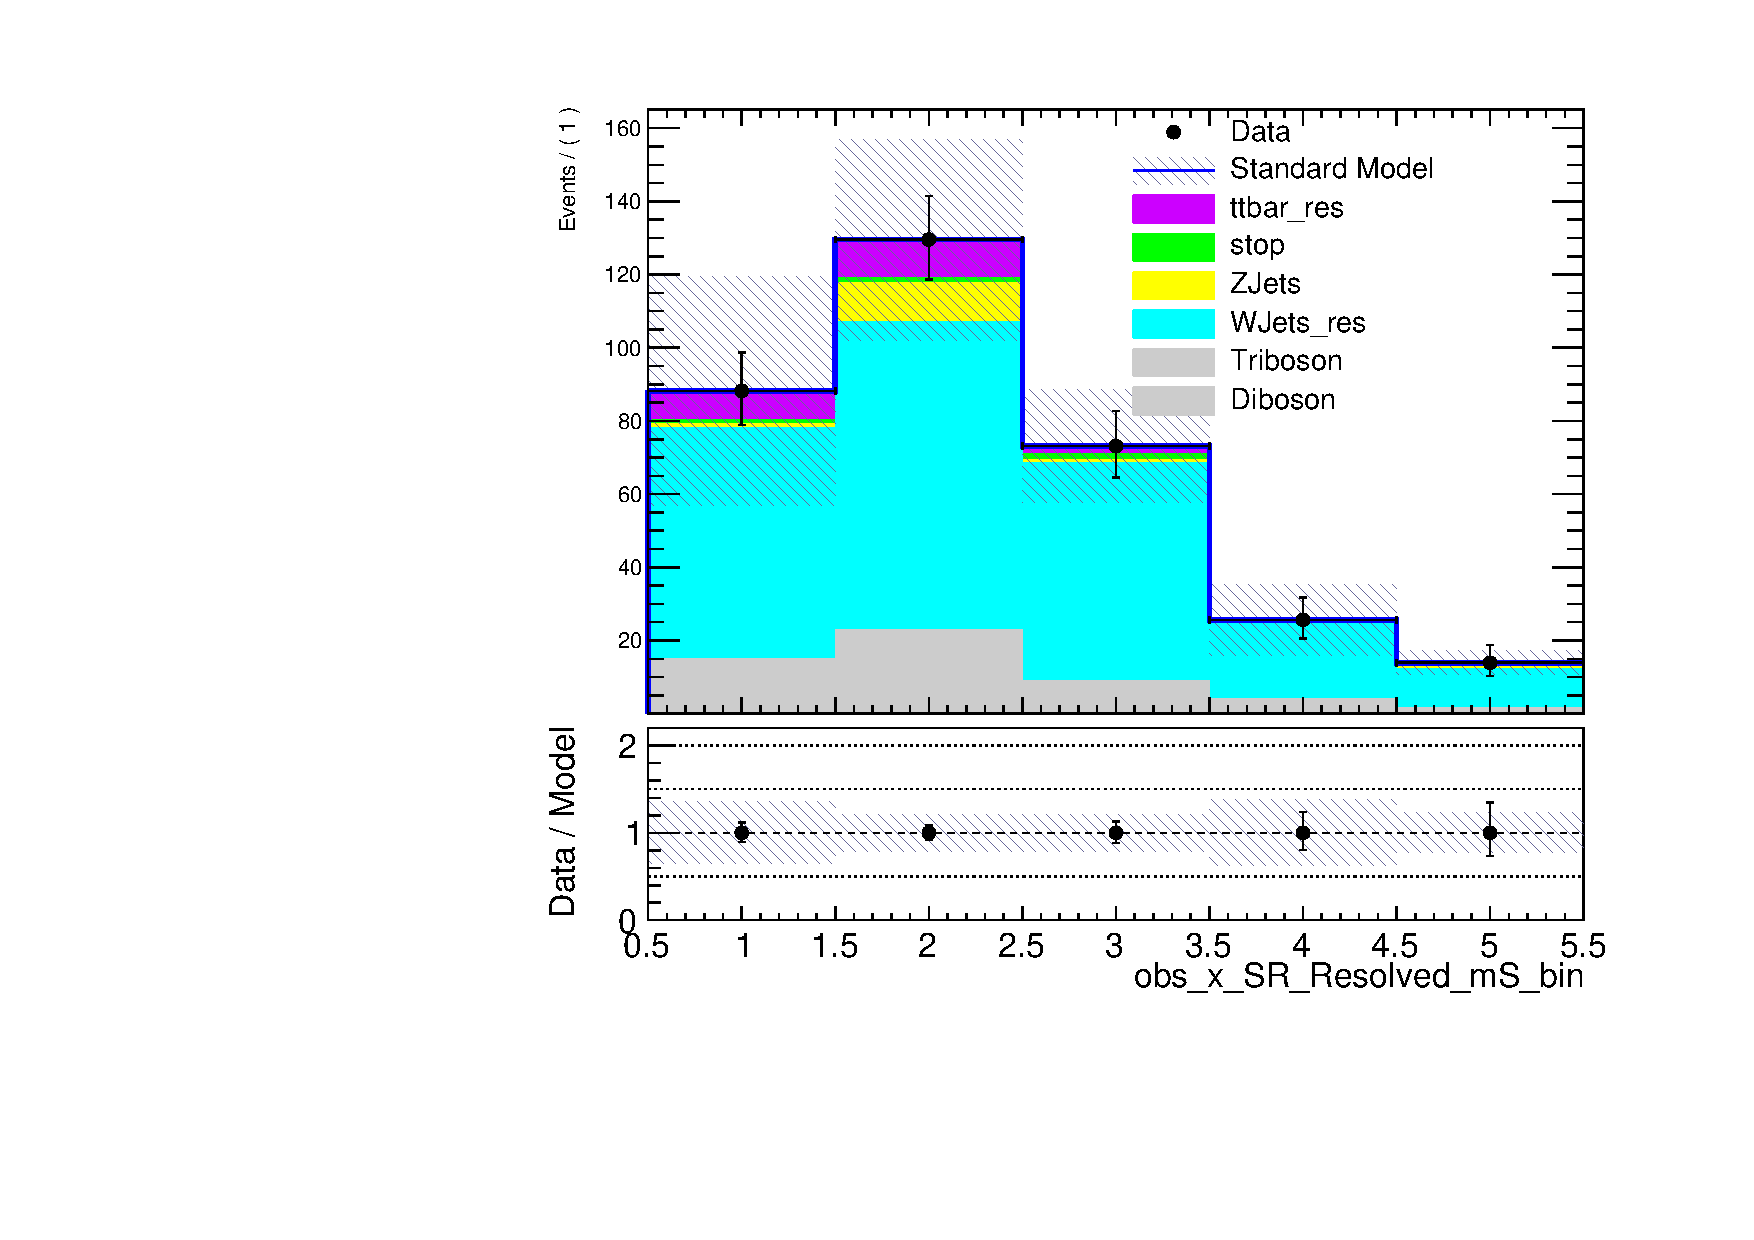
\includegraphics[width = 0.98\textwidth]{Figures/5/bkg_only/SR_Resolved_mS_bin_beforeFit.pdf}
	     \caption{Resolved SR pre-fit}
	     \end{subfigure}
	     \begin{subfigure}{0.49\textwidth}
	     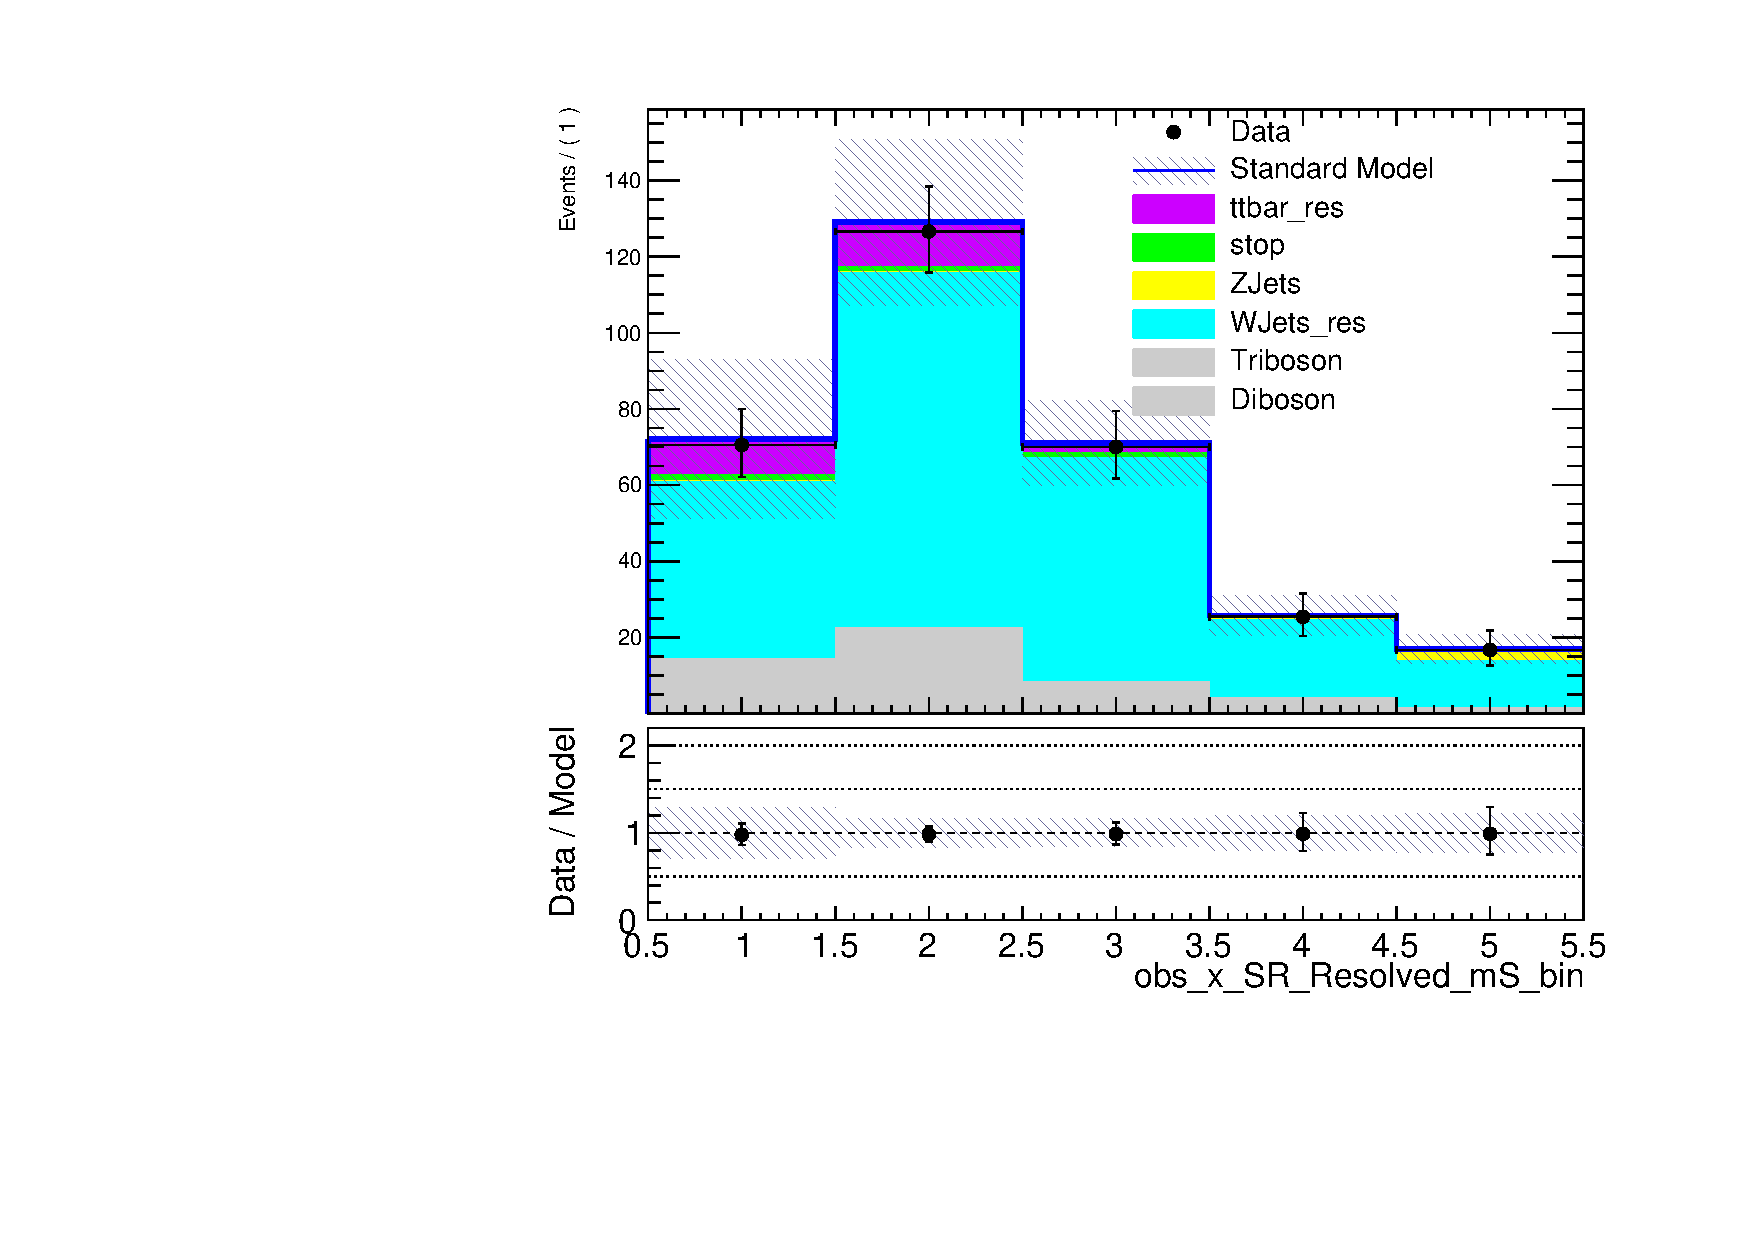
\includegraphics[width = 0.98\textwidth]{Figures/5/bkg_only/SR_Resolved_mS_bin_afterFit.pdf}
	     \caption{Resolved SR post-fit}
	     \end{subfigure}
	     \begin{subfigure}{0.49\textwidth}
	     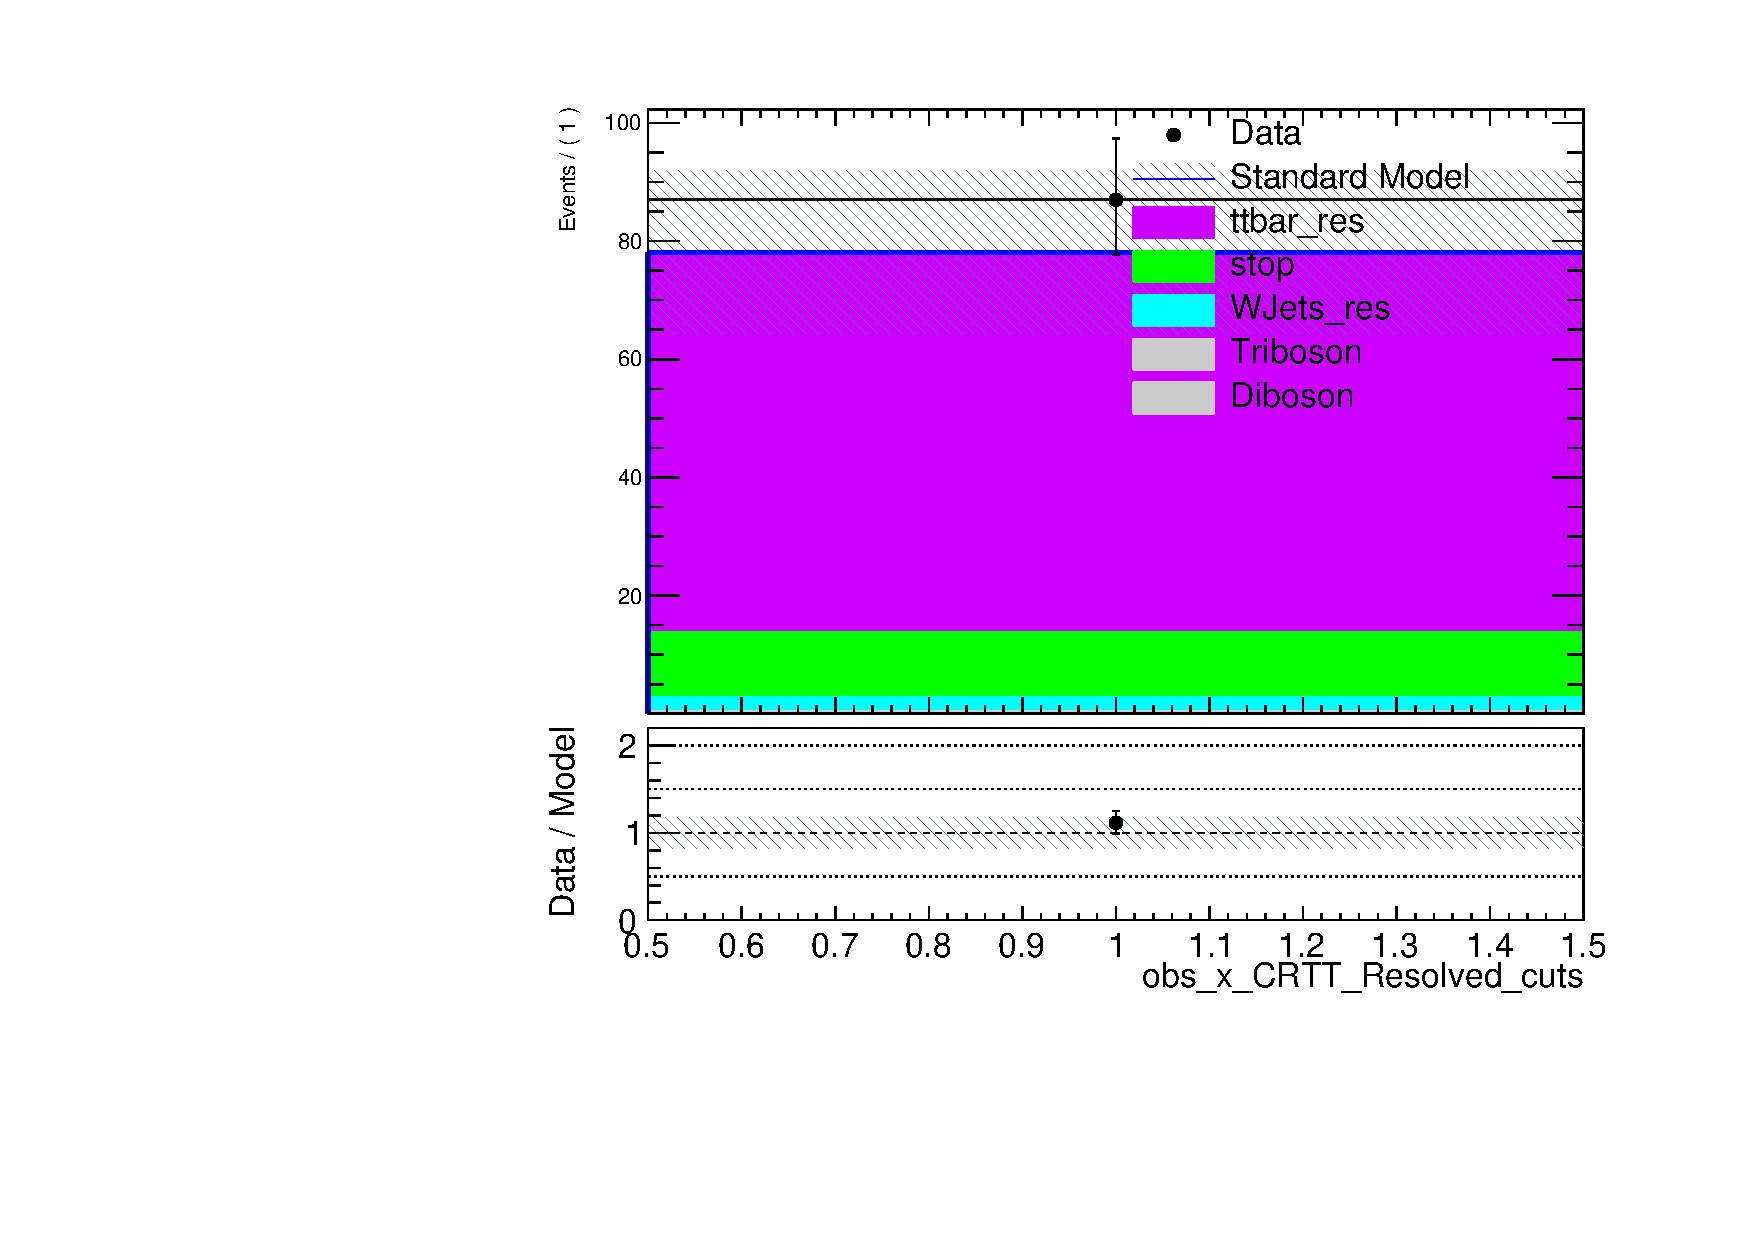
\includegraphics[width = 0.98\textwidth]{Figures/5/bkg_only/CRTT_Resolved_cuts_beforeFit.pdf}
	     \caption{Resolved CR \ttbar pre-fit}
	     \end{subfigure}
	     \begin{subfigure}{0.49\textwidth}
	     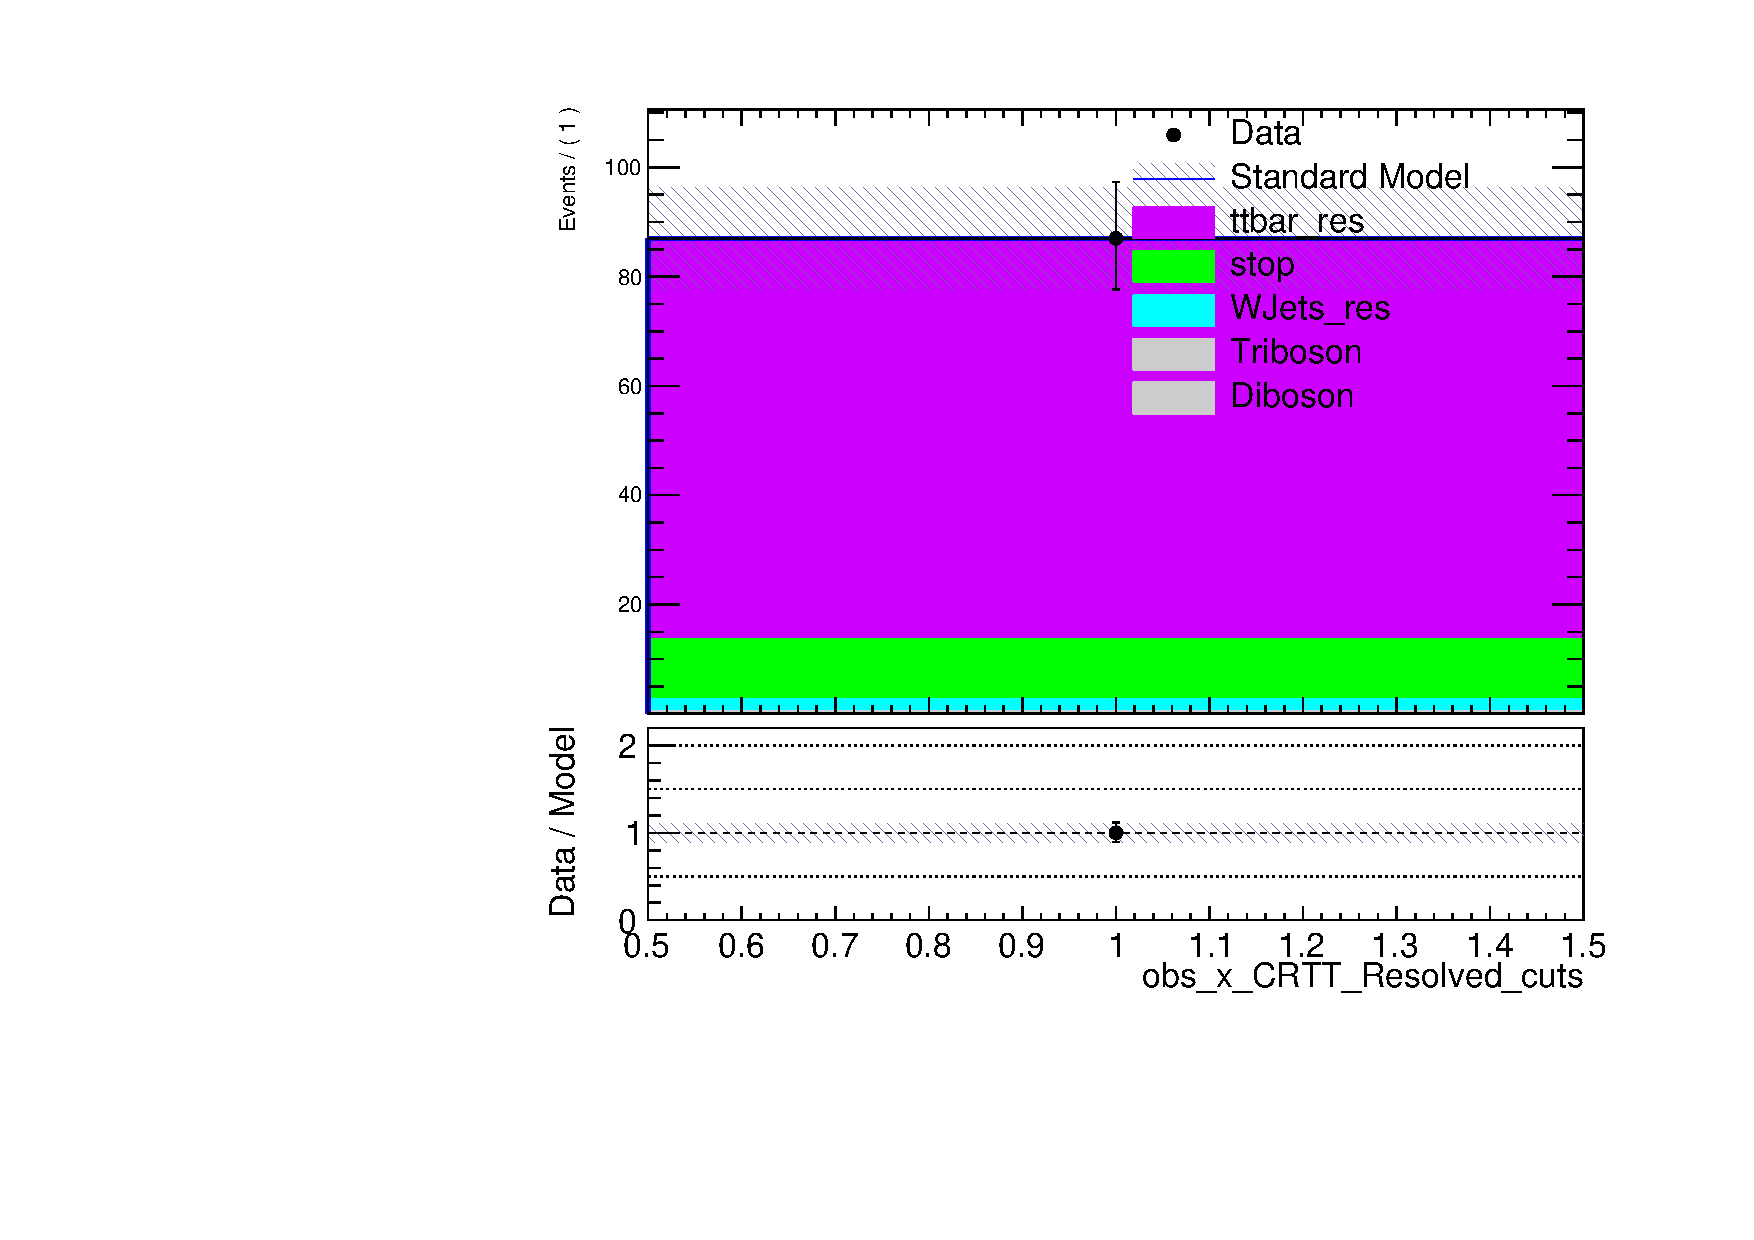
\includegraphics[width = 0.98\textwidth]{Figures/5/bkg_only/CRTT_Resolved_cuts_afterFit.pdf}
	     \caption{Resolved CR \ttbar post-fit}
	     \end{subfigure}
	     \begin{subfigure}{0.49\textwidth}
	     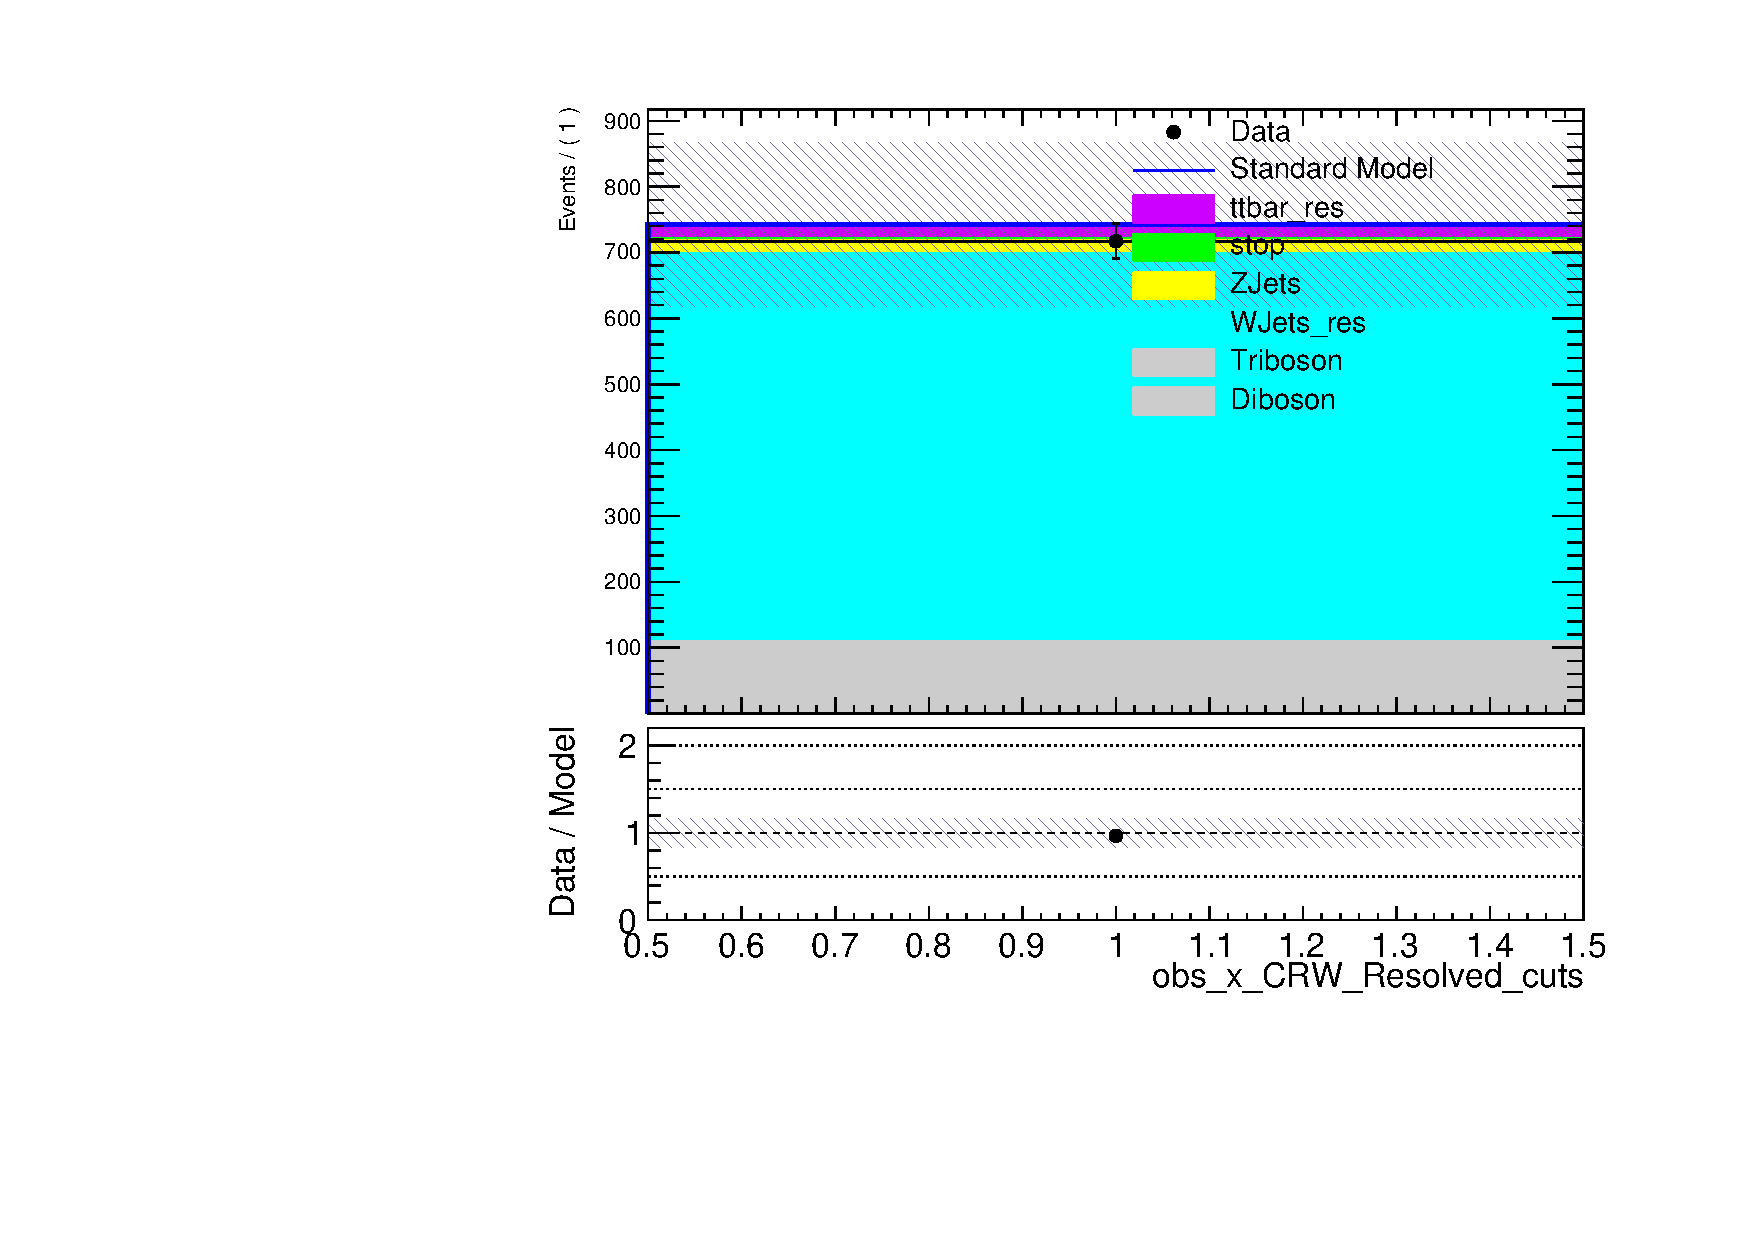
\includegraphics[width = 0.98\textwidth]{Figures/5/bkg_only/CRW_Resolved_cuts_beforeFit.pdf}
	     \caption{Resolved CR \wjets pre-fit}
	     \end{subfigure}
	     \begin{subfigure}{0.49\textwidth}
	     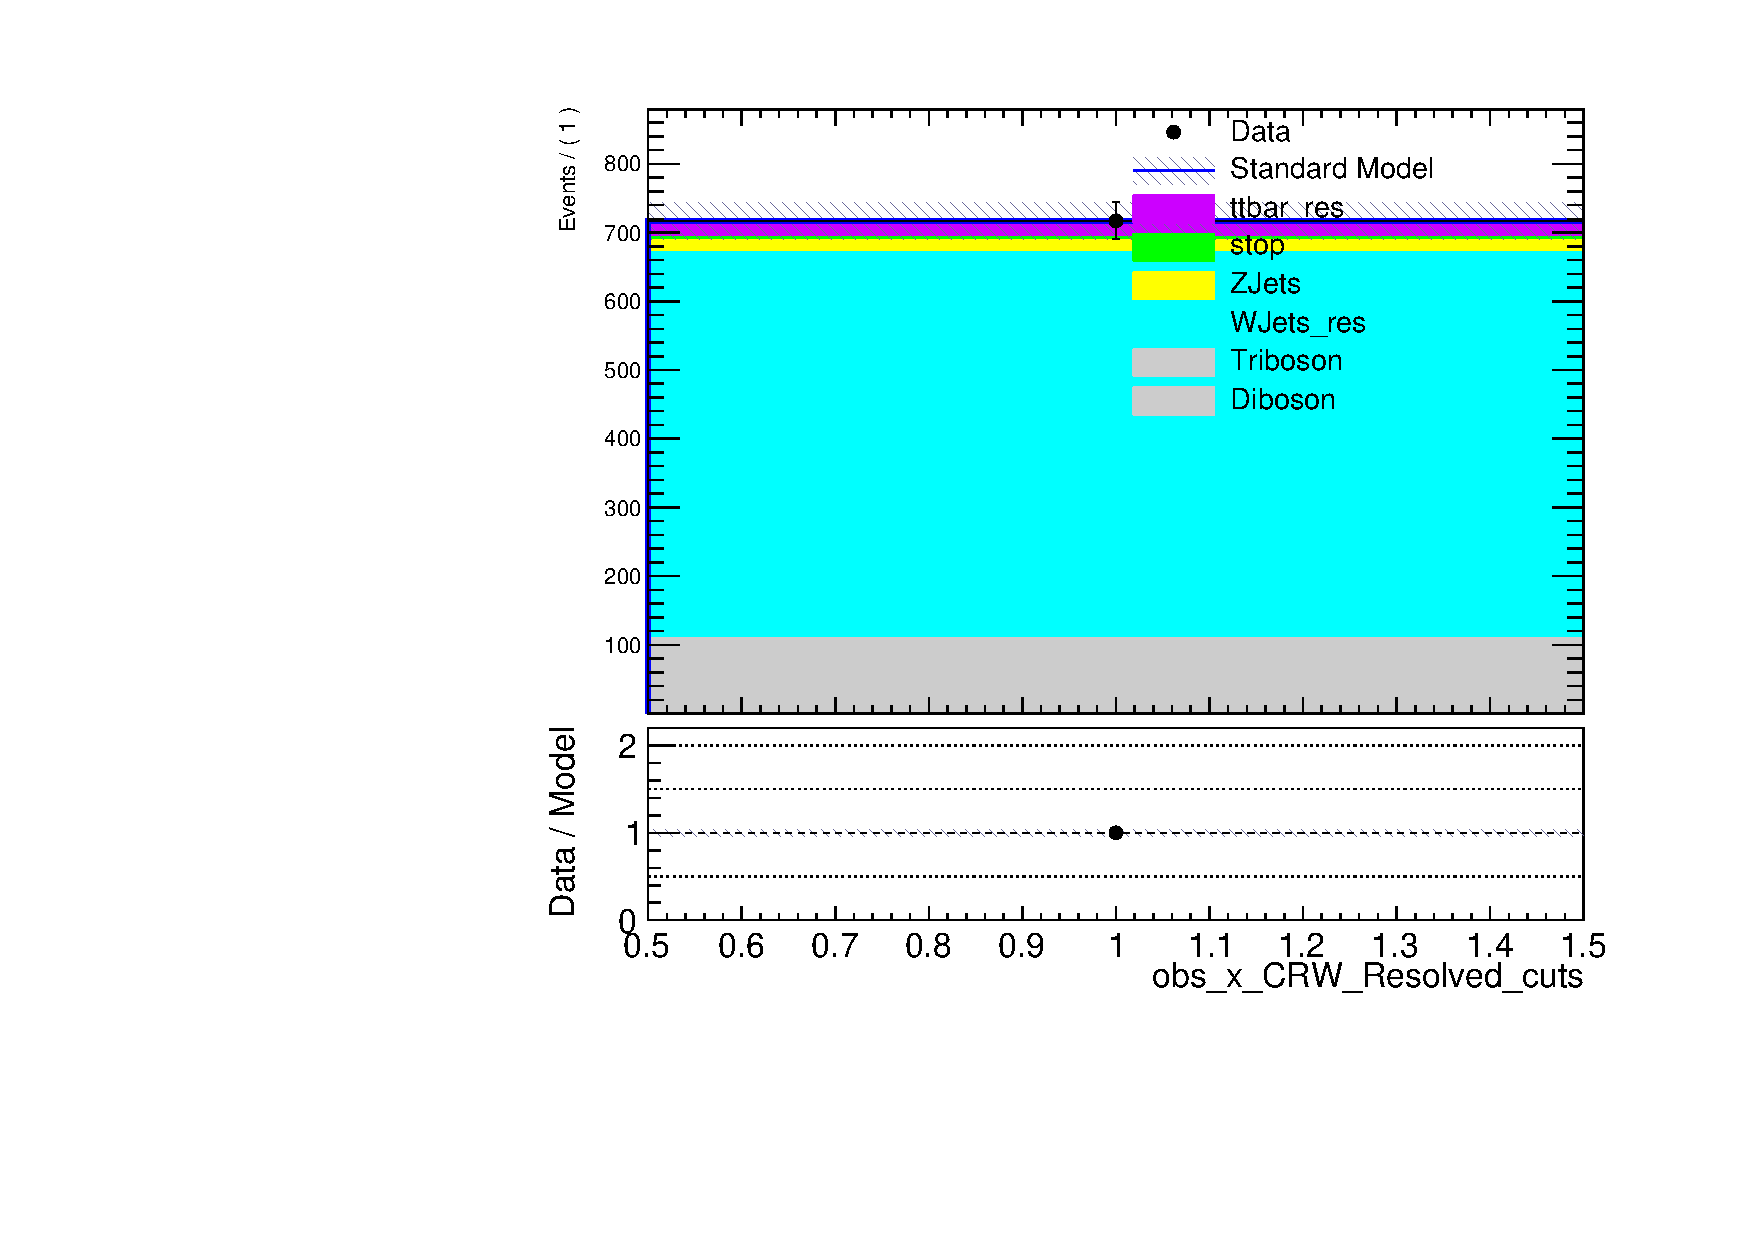
\includegraphics[width = 0.98\textwidth]{Figures/5/bkg_only/CRW_Resolved_cuts_afterFit.pdf}
	     \caption{Resolved CR \wjets post-fit}
	     \end{subfigure}

	     \caption{Pre and post-fit yields in the resolved signal and control regions for a background-only fit.}
	     \label{fig:bkg_only_res}
	  \end{figure}

    \begin{table}
\centering
\small
\begin{tabular*}{\textwidth}{@{\extracolsep{\fill}}lccc}
\toprule
\textbf{Uncertainty of channel}                                    & SR\_Merged            & CRW\_Merged            & CRTT\_Merged            \\
\midrule
%%
Total background expectation             &  $46.88$        &  $204.97$        &  $58.93$       \\
%% \\
\midrule
%%
Total statistical $(\sqrt{N_{\mathrm{exp}}})$              & $\pm 6.85$        & $\pm 14.32$        & $\pm 7.68$       \\
%%
Total background systematic               & $\pm 8.87\ [18.92\%] $        & $\pm 14.27\ [6.96\%] $        & $\pm 7.66\ [12.99\%] $             \\
\midrule
%%
\mu\_Wjets\_mgd         & $\pm 9.73$          & $\pm 43.69$          & $\pm 0.11$       \\
%%
\alpha\_WJetsTheorySys         & $\pm 6.78$          & $\pm 30.47$          & $\pm 0.07$       \\
%%
\gamma\_stat\_SR\_Merged\_mS\_bin\_0         & $\pm 4.42$          & $\pm 0.00$          & $\pm 0.00$       \\
%%
\gamma\_stat\_SR\_Merged\_mS\_bin\_1         & $\pm 2.78$          & $\pm 0.00$          & $\pm 0.00$       \\
%%
\alpha\_JET\_Flavor\_Response         & $\pm 1.63$          & $\pm 1.77$          & $\pm 1.92$       \\
%%
\gamma\_stat\_SR\_Merged\_mS\_bin\_2         & $\pm 1.56$          & $\pm 0.00$          & $\pm 0.00$       \\
%%
\alpha\_DibosonTheorySys         & $\pm 1.40$          & $\pm 5.50$          & $\pm 0.02$       \\
%%
\alpha\_JET\_Pileup\_PtTerm         & $\pm 1.33$          & $\pm 2.99$          & $\pm 2.82$       \\
%%
\alpha\_MET\_SoftTrk\_ResoPerp         & $\pm 1.04$          & $\pm 0.18$          & $\pm 0.02$       \\
%%
\alpha\_TRK\_FAKE\_RATE\_LR         & $\pm 1.00$          & $\pm 0.00$          & $\pm 0.01$       \\
%%
\alpha\_JET\_Flavor\_Composition         & $\pm 0.90$          & $\pm 2.96$          & $\pm 2.64$       \\
%%
\mu\_ttbar\_mgd         & $\pm 0.85$          & $\pm 1.99$          & $\pm 15.64$       \\
%%
\alpha\_JET\_EffectiveNP\_Mixed2         & $\pm 0.81$          & $\pm 2.97$          & $\pm 2.98$       \\
%%
\alpha\_lumiSys         & $\pm 0.79$          & $\pm 3.46$          & $\pm 1.00$       \\
%%
\alpha\_JET\_EtaIntercalibration\_TS         & $\pm 0.66$          & $\pm 2.93$          & $\pm 2.93$       \\
%%
\alpha\_JET\_Pileup\_OffsetNPV         & $\pm 0.66$          & $\pm 2.57$          & $\pm 2.67$       \\
%%
\alpha\_JET\_EtaIntercalibration\_M         & $\pm 0.64$          & $\pm 0.18$          & $\pm 0.00$       \\
%%
\alpha\_JET\_EffectiveNP\_Modelling1         & $\pm 0.59$          & $\pm 2.33$          & $\pm 2.73$       \\
%%
\alpha\_ttbarTheorySys         & $\pm 0.57$          & $\pm 1.32$          & $\pm 10.42$       \\
%%
\alpha\_JET\_Pileup\_RhoTopology         & $\pm 0.57$          & $\pm 2.53$          & $\pm 2.83$       \\
%%
\gamma\_stat\_SR\_Merged\_mS\_bin\_3         & $\pm 0.51$          & $\pm 0.00$          & $\pm 0.00$       \\
%%
\alpha\_JET\_Pileup\_OffsetMu         & $\pm 0.50$          & $\pm 0.02$          & $\pm 0.00$       \\
%%
\alpha\_MET\_SoftTrk\_ResoPara         & $\pm 0.46$          & $\pm 0.28$          & $\pm 0.84$       \\
		%%
		\bottomrule
		\end{tabular*}
		\caption{Effect of systematic uncertainties in the merged signal and control regions for a background-only fit. Uncertainties with a magnitude <1\% of total yield are excluded.}
		\label{tab:systs_mgd}
		\end{table}

    \begin{table}
\centering
\small
\begin{tabular*}{\textwidth}{@{\extracolsep{\fill}}lccc}
\toprule
\textbf{Uncertainty of channel}                                    & SR\_Resolved            & CRW\_Resolved            & CRTT\_Resolved            \\
\midrule
%%
Total background expectation             &  $314.82$        &  $717.05$        &  $87.06$       \\
%% \\
\midrule
%%
Total statistical $(\sqrt{N_{\mathrm{exp}}})$              & $\pm 17.74$        & $\pm 26.78$        & $\pm 9.33$       \\
%%
Total background systematic               & $\pm 35.79\ [11.37\%] $        & $\pm 26.75\ [3.73\%] $        & $\pm 9.30\ [10.69\%] $             \\
\midrule
%%
\mu\_Wjets\_res         & $\pm 51.41$          & $\pm 125.23$          & $\pm 0.98$       \\
%%
\alpha\_WJetsTheorySys         & $\pm 46.08$          & $\pm 112.24$          & $\pm 0.88$       \\
%%
\gamma\_stat\_SR\_Resolved\_mS\_bin\_0         & $\pm 15.91$          & $\pm 0.00$          & $\pm 0.00$       \\
%%
\gamma\_stat\_SR\_Resolved\_mS\_bin\_1         & $\pm 14.84$          & $\pm 0.00$          & $\pm 0.00$       \\
%%
\alpha\_DibosonTheorySys         & $\pm 9.73$          & $\pm 20.94$          & $\pm 0.12$       \\
%%
\alpha\_JET\_Pileup\_PtTerm         & $\pm 9.72$          & $\pm 1.36$          & $\pm 0.00$       \\
%%
\gamma\_stat\_SR\_Resolved\_mS\_bin\_2         & $\pm 9.17$          & $\pm 0.00$          & $\pm 0.00$       \\
%%
\alpha\_MET\_SoftTrk\_ResoPerp         & $\pm 7.09$          & $\pm 0.19$          & $\pm 0.17$       \\
%%
\alpha\_JET\_Pileup\_OffsetNPV         & $\pm 6.56$          & $\pm 1.26$          & $\pm 0.19$       \\
%%
\mu\_ttbar\_res         & $\pm 6.39$          & $\pm 5.94$          & $\pm 19.36$       \\
%%
\alpha\_JET\_EtaIntercalibration\_TS         & $\pm 5.79$          & $\pm 1.31$          & $\pm 0.21$       \\
%%
\alpha\_lumiSys         & $\pm 5.32$          & $\pm 12.11$          & $\pm 1.47$       \\
%%
\alpha\_JET\_EffectiveNP\_Modelling1         & $\pm 5.08$          & $\pm 2.87$          & $\pm 0.35$       \\
%%
\alpha\_MET\_SoftTrk\_Scale         & $\pm 4.92$          & $\pm 0.05$          & $\pm 0.07$       \\
%%
\alpha\_ttbarTheorySys         & $\pm 4.78$          & $\pm 4.45$          & $\pm 14.50$       \\
%%
\alpha\_JET\_EffectiveNP\_Mixed2         & $\pm 3.90$          & $\pm 1.40$          & $\pm 0.01$       \\
%%
\gamma\_stat\_SR\_Resolved\_mS\_bin\_3         & $\pm 3.66$          & $\pm 0.00$          & $\pm 0.00$       \\
%%
\alpha\_JET\_Pileup\_OffsetMu         & $\pm 3.60$          & $\pm 1.75$          & $\pm 2.00$       \\
%%
\gamma\_stat\_SR\_Resolved\_mS\_bin\_4         & $\pm 3.54$          & $\pm 0.00$          & $\pm 0.00$       \\
		%%
		\bottomrule
		\end{tabular*}
		\caption{Effect of systematic uncertainties in the resolved signal and control regions for a background-only fit. Uncertainties with a magnitude <1\% of total yield are excluded.}
		\label{tab:systs_res}
		\end{table}

\FloatBarrier
\subsection{Exclusion Fit}
I finally perform an exclusion fit using the signal model. I evaluate the $\text{CL}_\text{s}$ for the nominal signal strength $\mu_\text{sig} = 1$ for each signal mass point in the \ms-\mZp plane, and interpolate between mass points using a cubic interpolation. The signal regions remain blinded, so I once again replace ATLAS data with Asimov data equal to the nearest integer value to the pre-fit MC expected SM yield in those regions. I then build a contour along $\text{CL}_\text{s} = 0.05$, and the area outside this contour ($\text{CL}_\text{s} > 0.05$) would be excluded at a 95\% confidence level with the Asimov data. This provides the strongest estimate of the designed regions' sensitivity to the dark Higgs signal model prior to unblinding.

I first perform an exclusion fit on the \merged analysis channel alone to assess the sensitivity of the \merged signal region selection criteria I designed. The expected exclusion contour for the \merged channel is shown in Figure \ref{fig:excl_mgd}. I then perform an exclusion fit of the \resolved channel alone, with the expected exclusion contour shown in Figure \ref{fig:excl_res} to see how it complements the \merged channel. Finally, in Figure \ref{fig:excl_comb} I show the expected exclusion contour for the combined \merged and \resolved channels, demonstrating the full expected exclusion power of the analysis. Figure \ref{fig:had_sens} shows the expected and observed exclusion limits obtained in the fully hadronic $s\rightarrow WW$ decay channel for comparison.

The expected exclusion contours show that the merged region dominates sensitivity. On its own, the resolved region has very little exclusion power, but it helps to complement and strengthen the results from the merged region. As a result, we expect to substantially improve on the limits set in the fully hadronic decay channel in our analysis.

\begin{figure}[h]
    \centering
    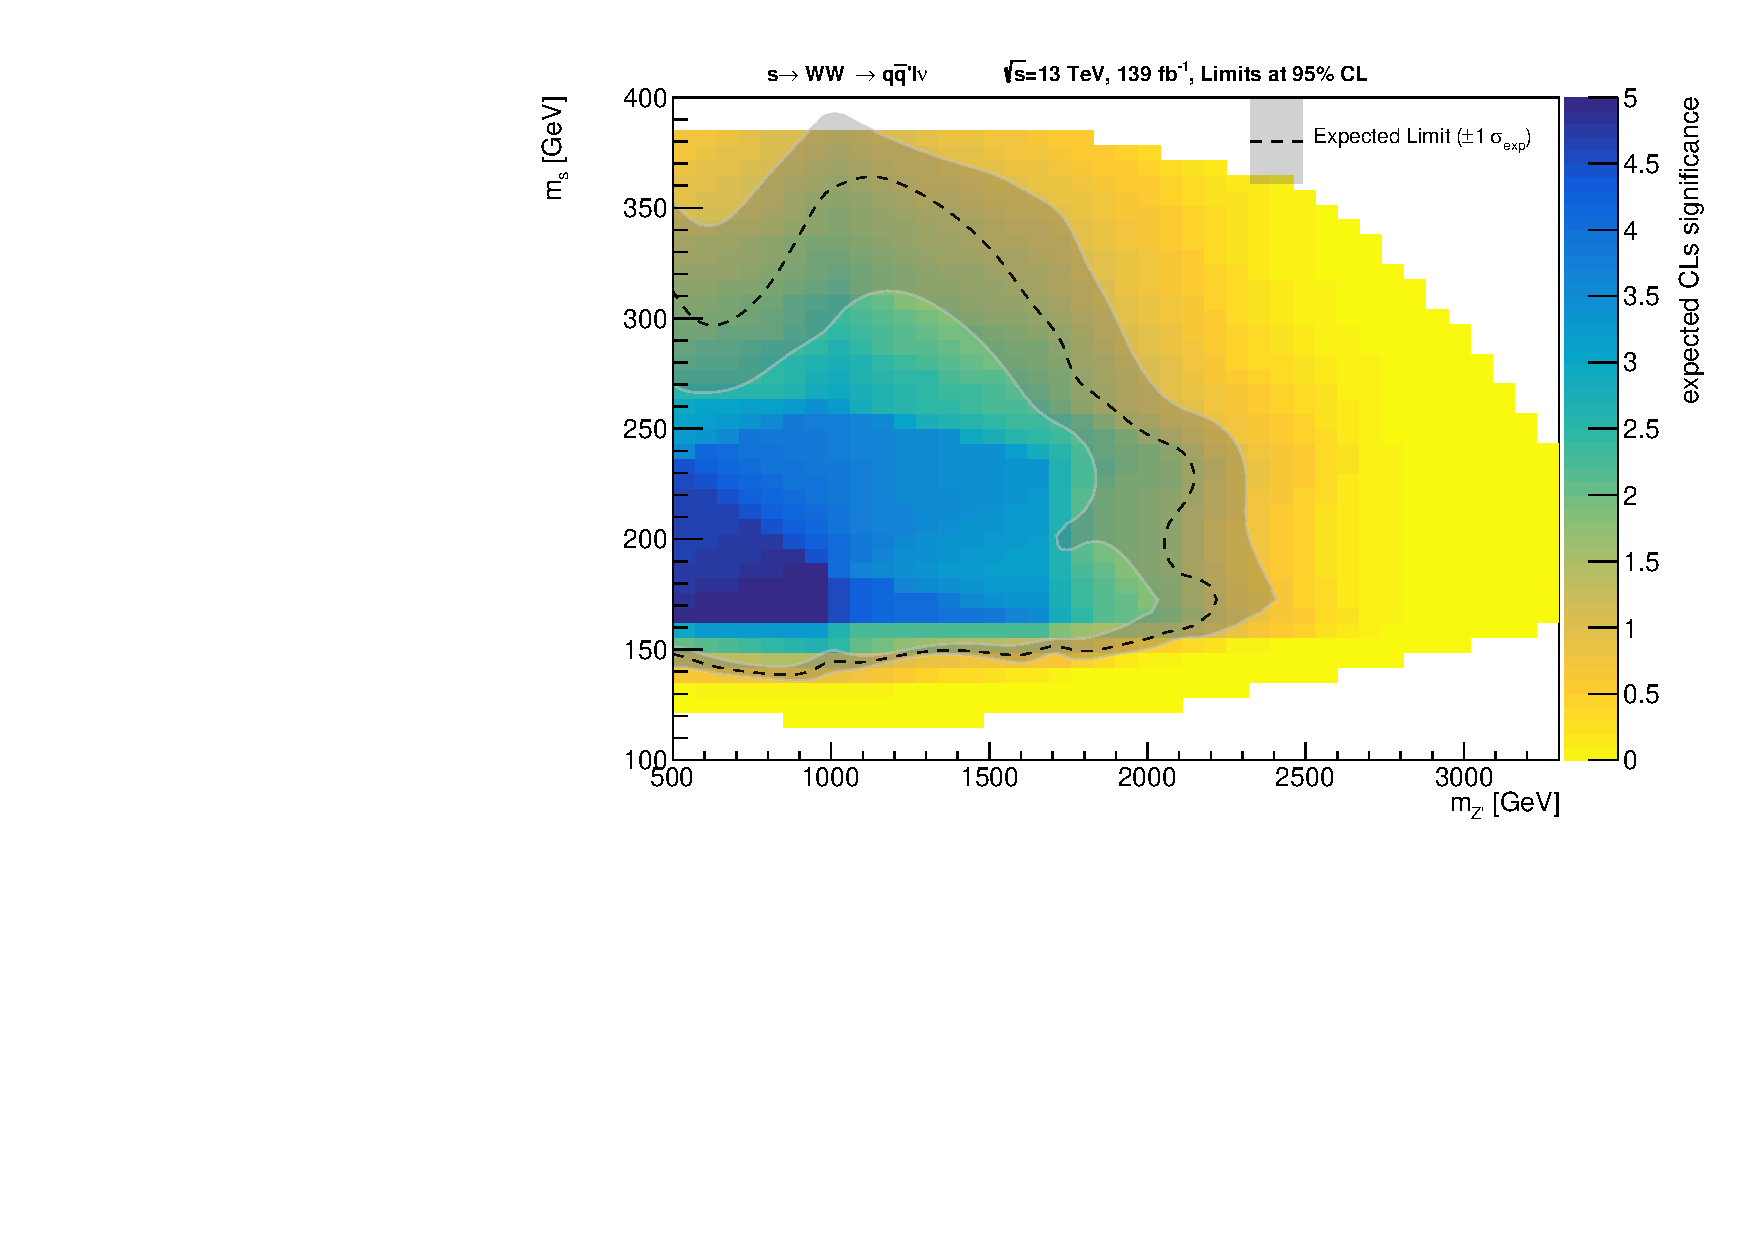
\includegraphics[width=0.8\textwidth]{Figures/5/fits/MERGED.pdf}
    \caption{Expected exclusion limits for the dark Higgs signal model obtained using the \merged signal and control regions.}
    \label{fig:excl_mgd}
\end{figure}

\begin{figure}[h]
    \centering
    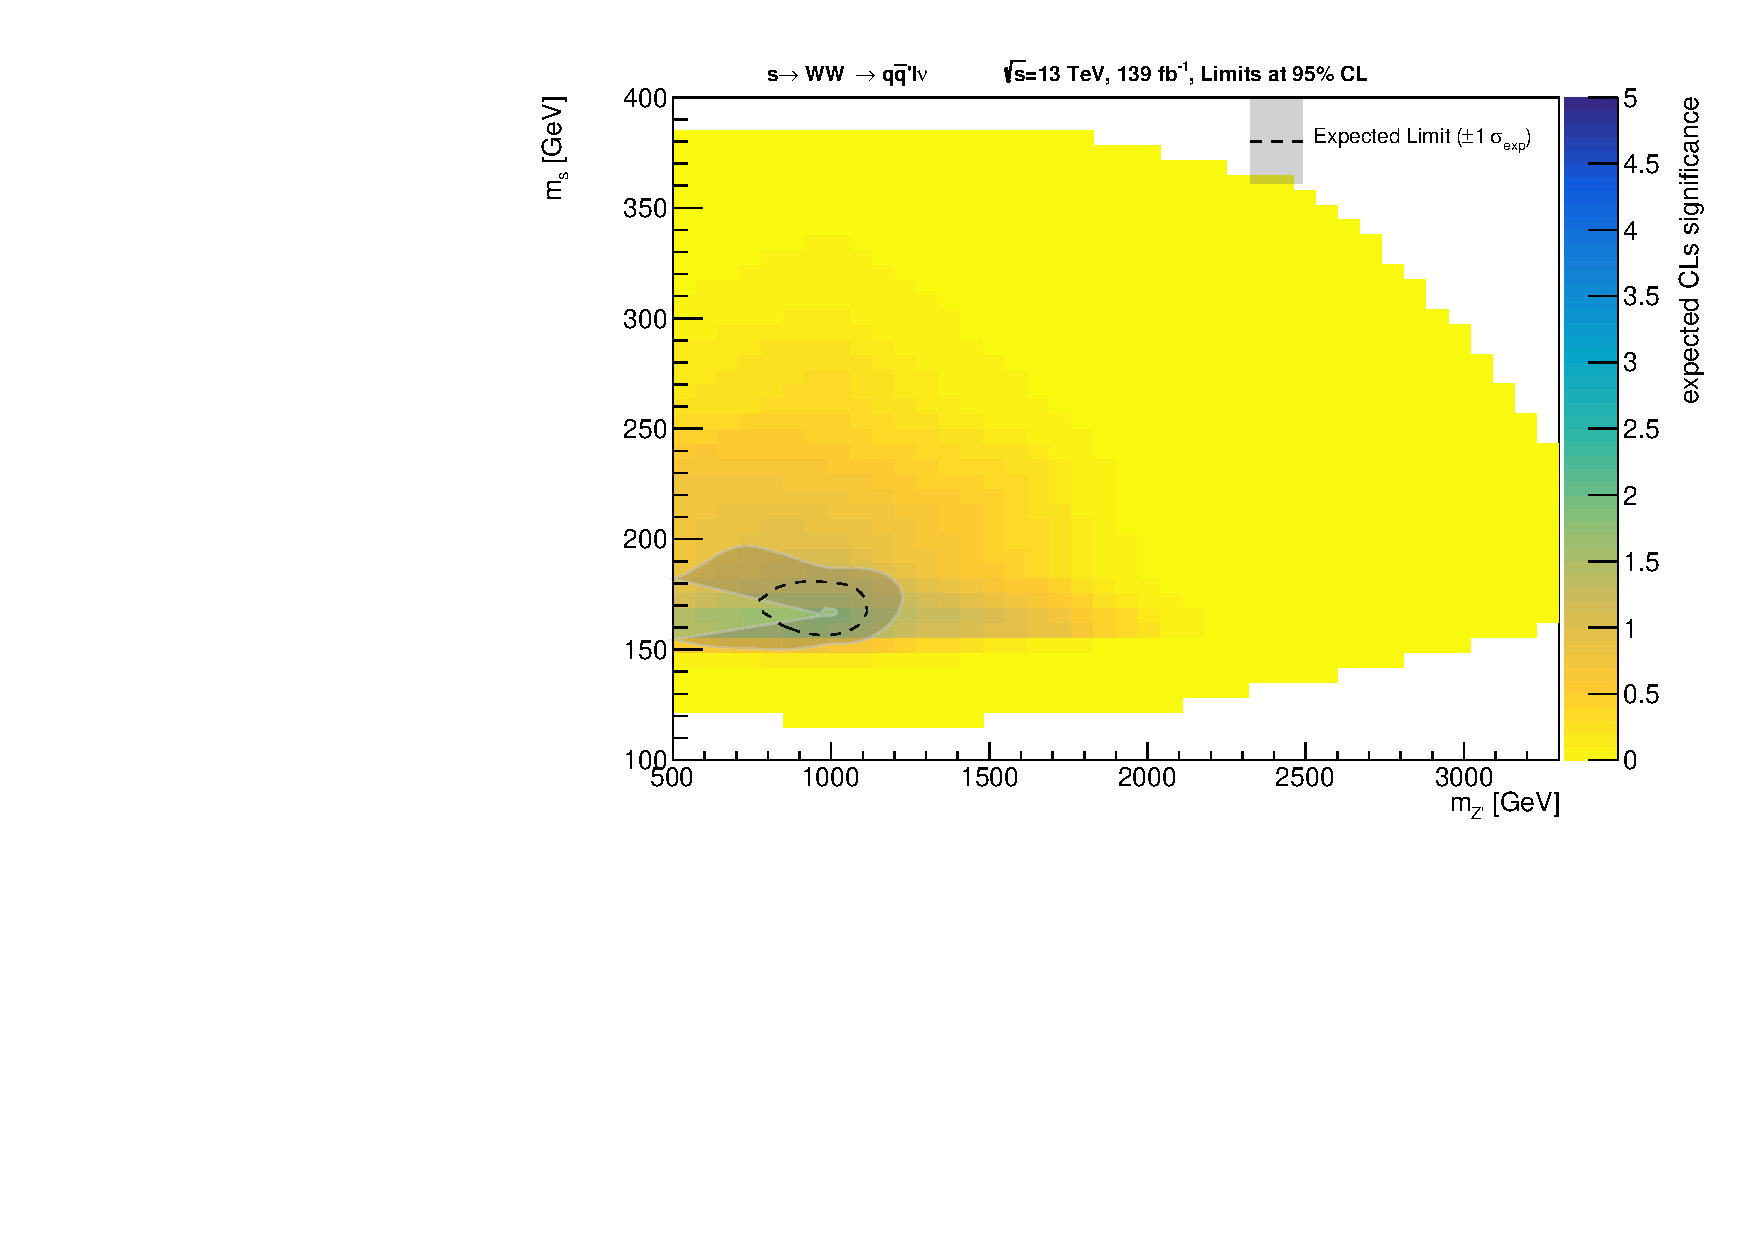
\includegraphics[width=0.8\textwidth]{Figures/5/fits/RESOLVED.pdf}
    \caption{Expected exclusion limits for the dark Higgs signal model obtained using the \resolved signal and control regions.}
    \label{fig:excl_res}
\end{figure}

\begin{figure}[h]
    \centering
    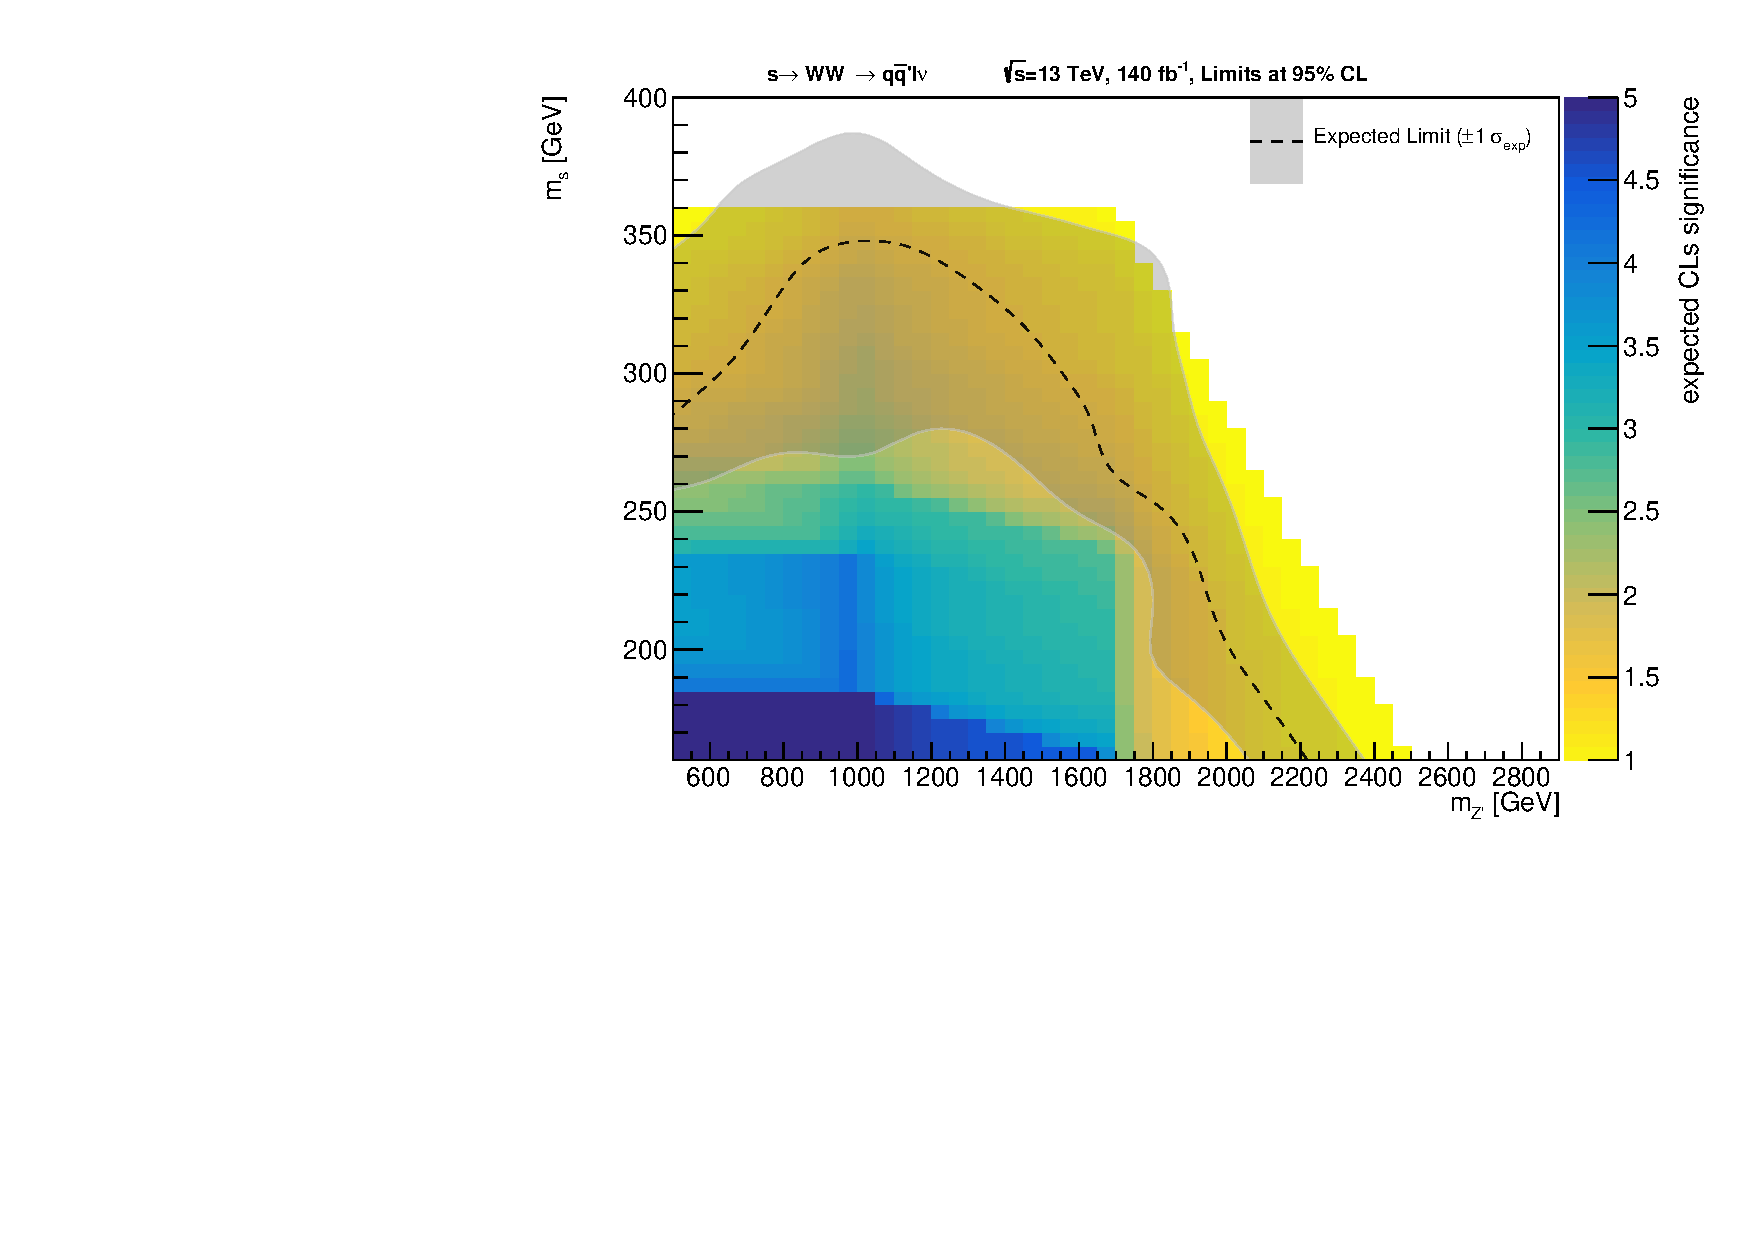
\includegraphics[width=0.8\textwidth]{Figures/5/fits/COMBO.pdf}
    \caption{Expected exclusion limits for the dark Higgs signal model obtained using the \merged and \resolved signal and control regions.}
    \label{fig:excl_comb}
\end{figure}

\begin{figure}[h]
    \centering
    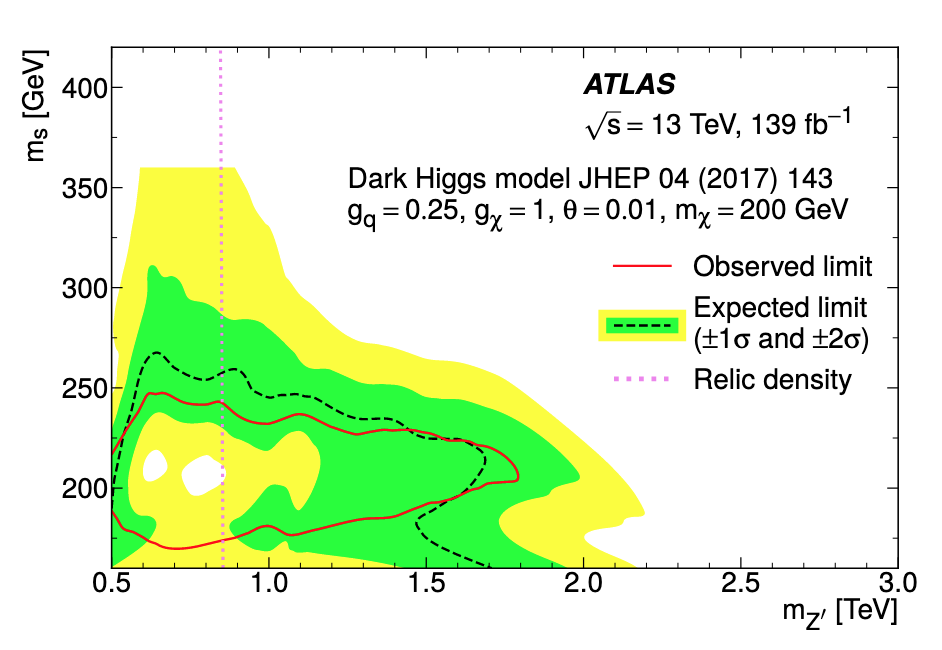
\includegraphics[width=0.8\textwidth]{Figures/5/had_analy_contour.png}
    \caption{Expected and observed exclusion limits for the dark Higgs signal model from the fully hadronic $s\rightarrow WW$ channel from \cite{had_analy}.}
    \label{fig:had_sens}
\end{figure}

	\startchapter{Conclusions}
\label{concl}
This thesis has presented the design of the most sensitive ``merged" signal region in the search for dark matter produced with a new heavy vector boson, $Z'$, and a scalar ``dark Higgs" boson, $s$, decaying to a pair of $W$ bosons with a semileptonic ($q\bar{q}\ell\nu$) final state. It has also presented the design of control regions to constrain the \ttbar SM background, as well as the important supporting analysis work.  The search uses data collected by the ATLAS experiment in 2015-2018, from proton-proton collisions at a center-of-mass energy of 13 TeV.

The search for the dark Higgs model \cite{Hunting} is motivated by the desire to detect and characterize dark matter, as well as the requirement of a mechanism to generate the masses of particles in the dark sector. The SM is an extremely successful theory of the fundamental particles and their interactions, however astrophysical observations demand the existence of dark matter beyond the current confines of the model. The dark Higgs model introduces dark matter as a Majorana fermion, with a mass generated by the Higgs mechanism from a new Higgs field with an associated dark Higgs boson $s$. Through the mixing of the SM Higgs field and the dark Higgs field, the $s$ can interact with all massive SM particles and can thus decay to SM final states that are observable in the ATLAS detector.

To search for this signature, we have analyzed proton-proton collision events measured in the ATLAS detector. We have begun by defining a set of physics objects representing particles and groups of particles in the ATLAS detector. We have then used those definitions to reconstruct and characterize events in the ATLAS detector. Using the reconstructed events we have defined a signal region consisting of an optimized set of event-by-event criteria that, based on MC simulated data, are expected to have a high efficiency for selecting events containing signal (mono-$s$ decay) processes, and to select few SM background events.

We have subsequently defined the control regions as regions near to, but not overlapping with, the signal regions, which are statistically dominated by the \ttbar background process. We compared the MC simulated SM background to the measured ATLAS data in these regions to gain information about the accuracy of our MC predictions and constrain our predictions in the signal region. Based on the SM and signal predictions given by MC in the signal region, and the constraints derived in the control regions, we have finally calculated and presented the expected sensitivity of the signal regions to the signal model, which represents our ability to make conclusions about its existence using observations in those regions.

Using the designed regions described in this thesis, the search for the semileptonic $s$ decay will be able to substantially improve upon the sensitivity to the dark Higgs model achieved by prior searches in other decay channels. As shown in Figure \ref{fig:excl_comb} in the previous chapter, in this search we will be able to exclude $s$ masses from approximately 150 GeV up to a range between approximately 290 to 360 GeV, with $Z^\prime$ masses up to a range between approximately 1200 to 2200 GeV, using the Run-2 ATLAS 140 $\text{fb}^{-1}$ dataset at the proton-proton center-of-mass energy of 13 TeV.

	\appendix
	\startappendix{Additional Information}
\label{chapter:appendix}

\section{Preselection level plots}
\label{section:preselection}
\begin{figure}[htbp]
  \centering

     \begin{subfigure}{0.49\textwidth}
     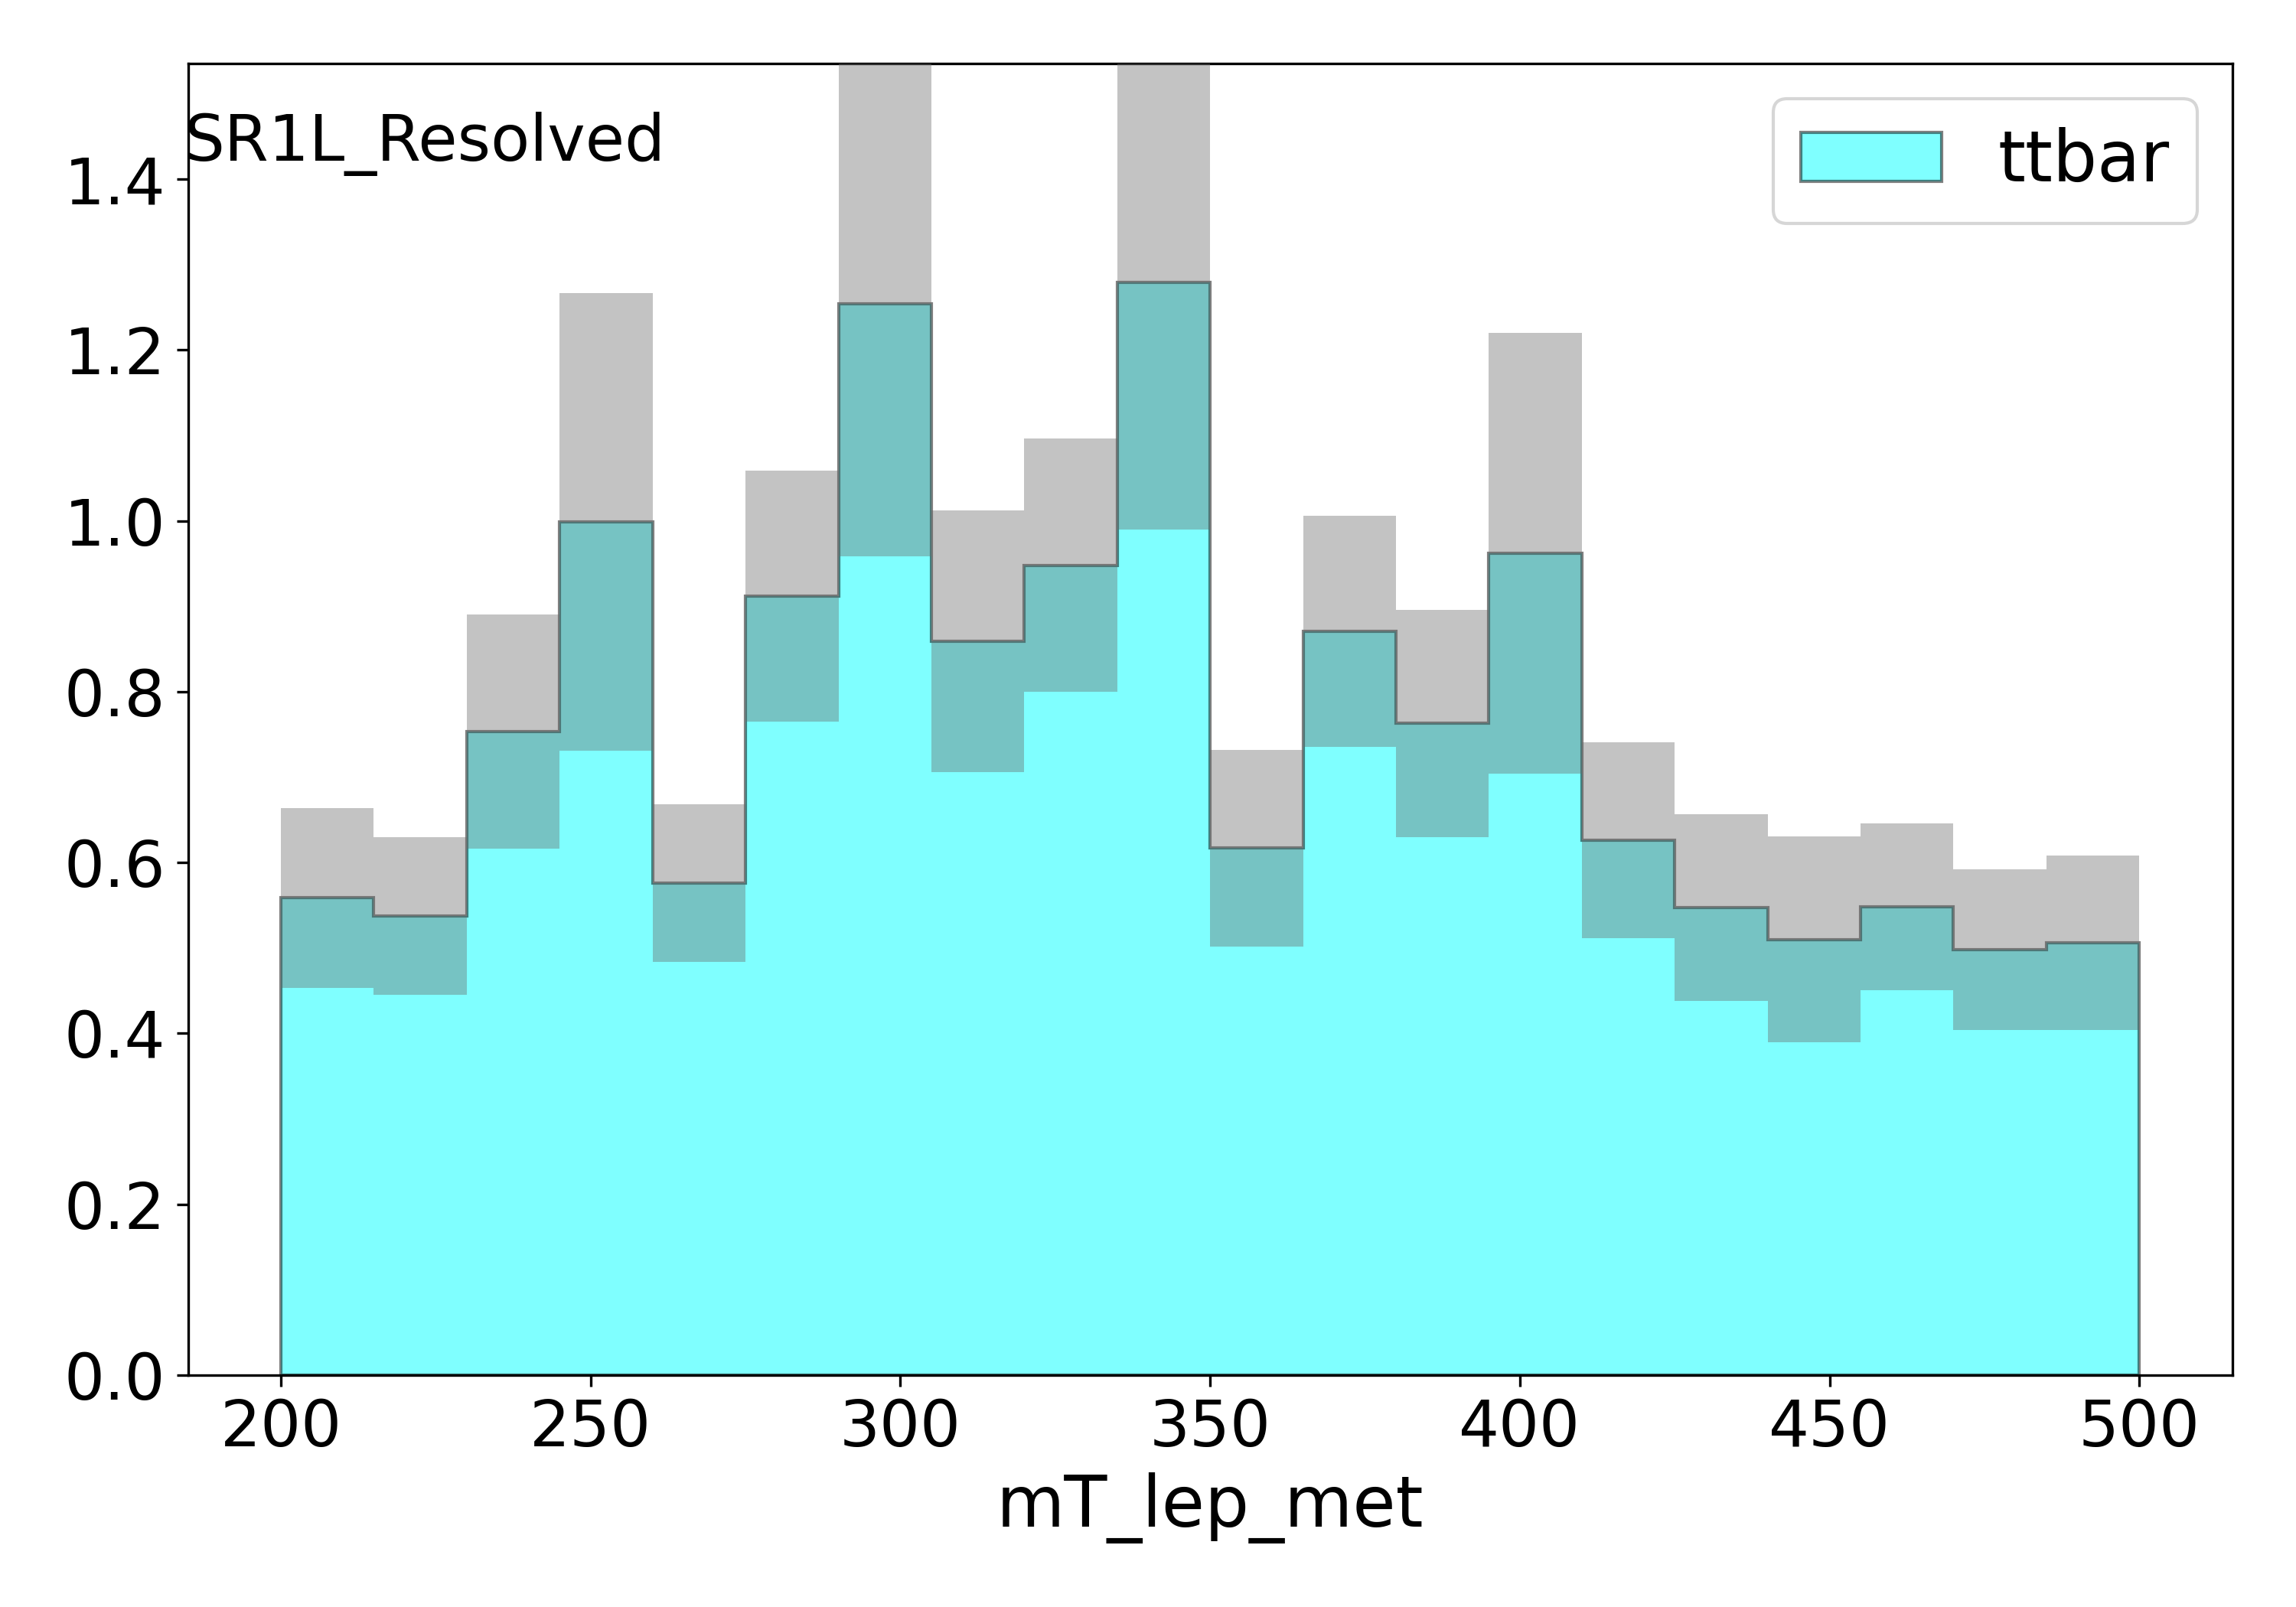
\includegraphics[width = 0.98\textwidth]{Figures/appendix/Preselection/mT_lep_met.png}
     \caption{\mtlepmet}
     \end{subfigure}
     \begin{subfigure}{0.49\textwidth}
     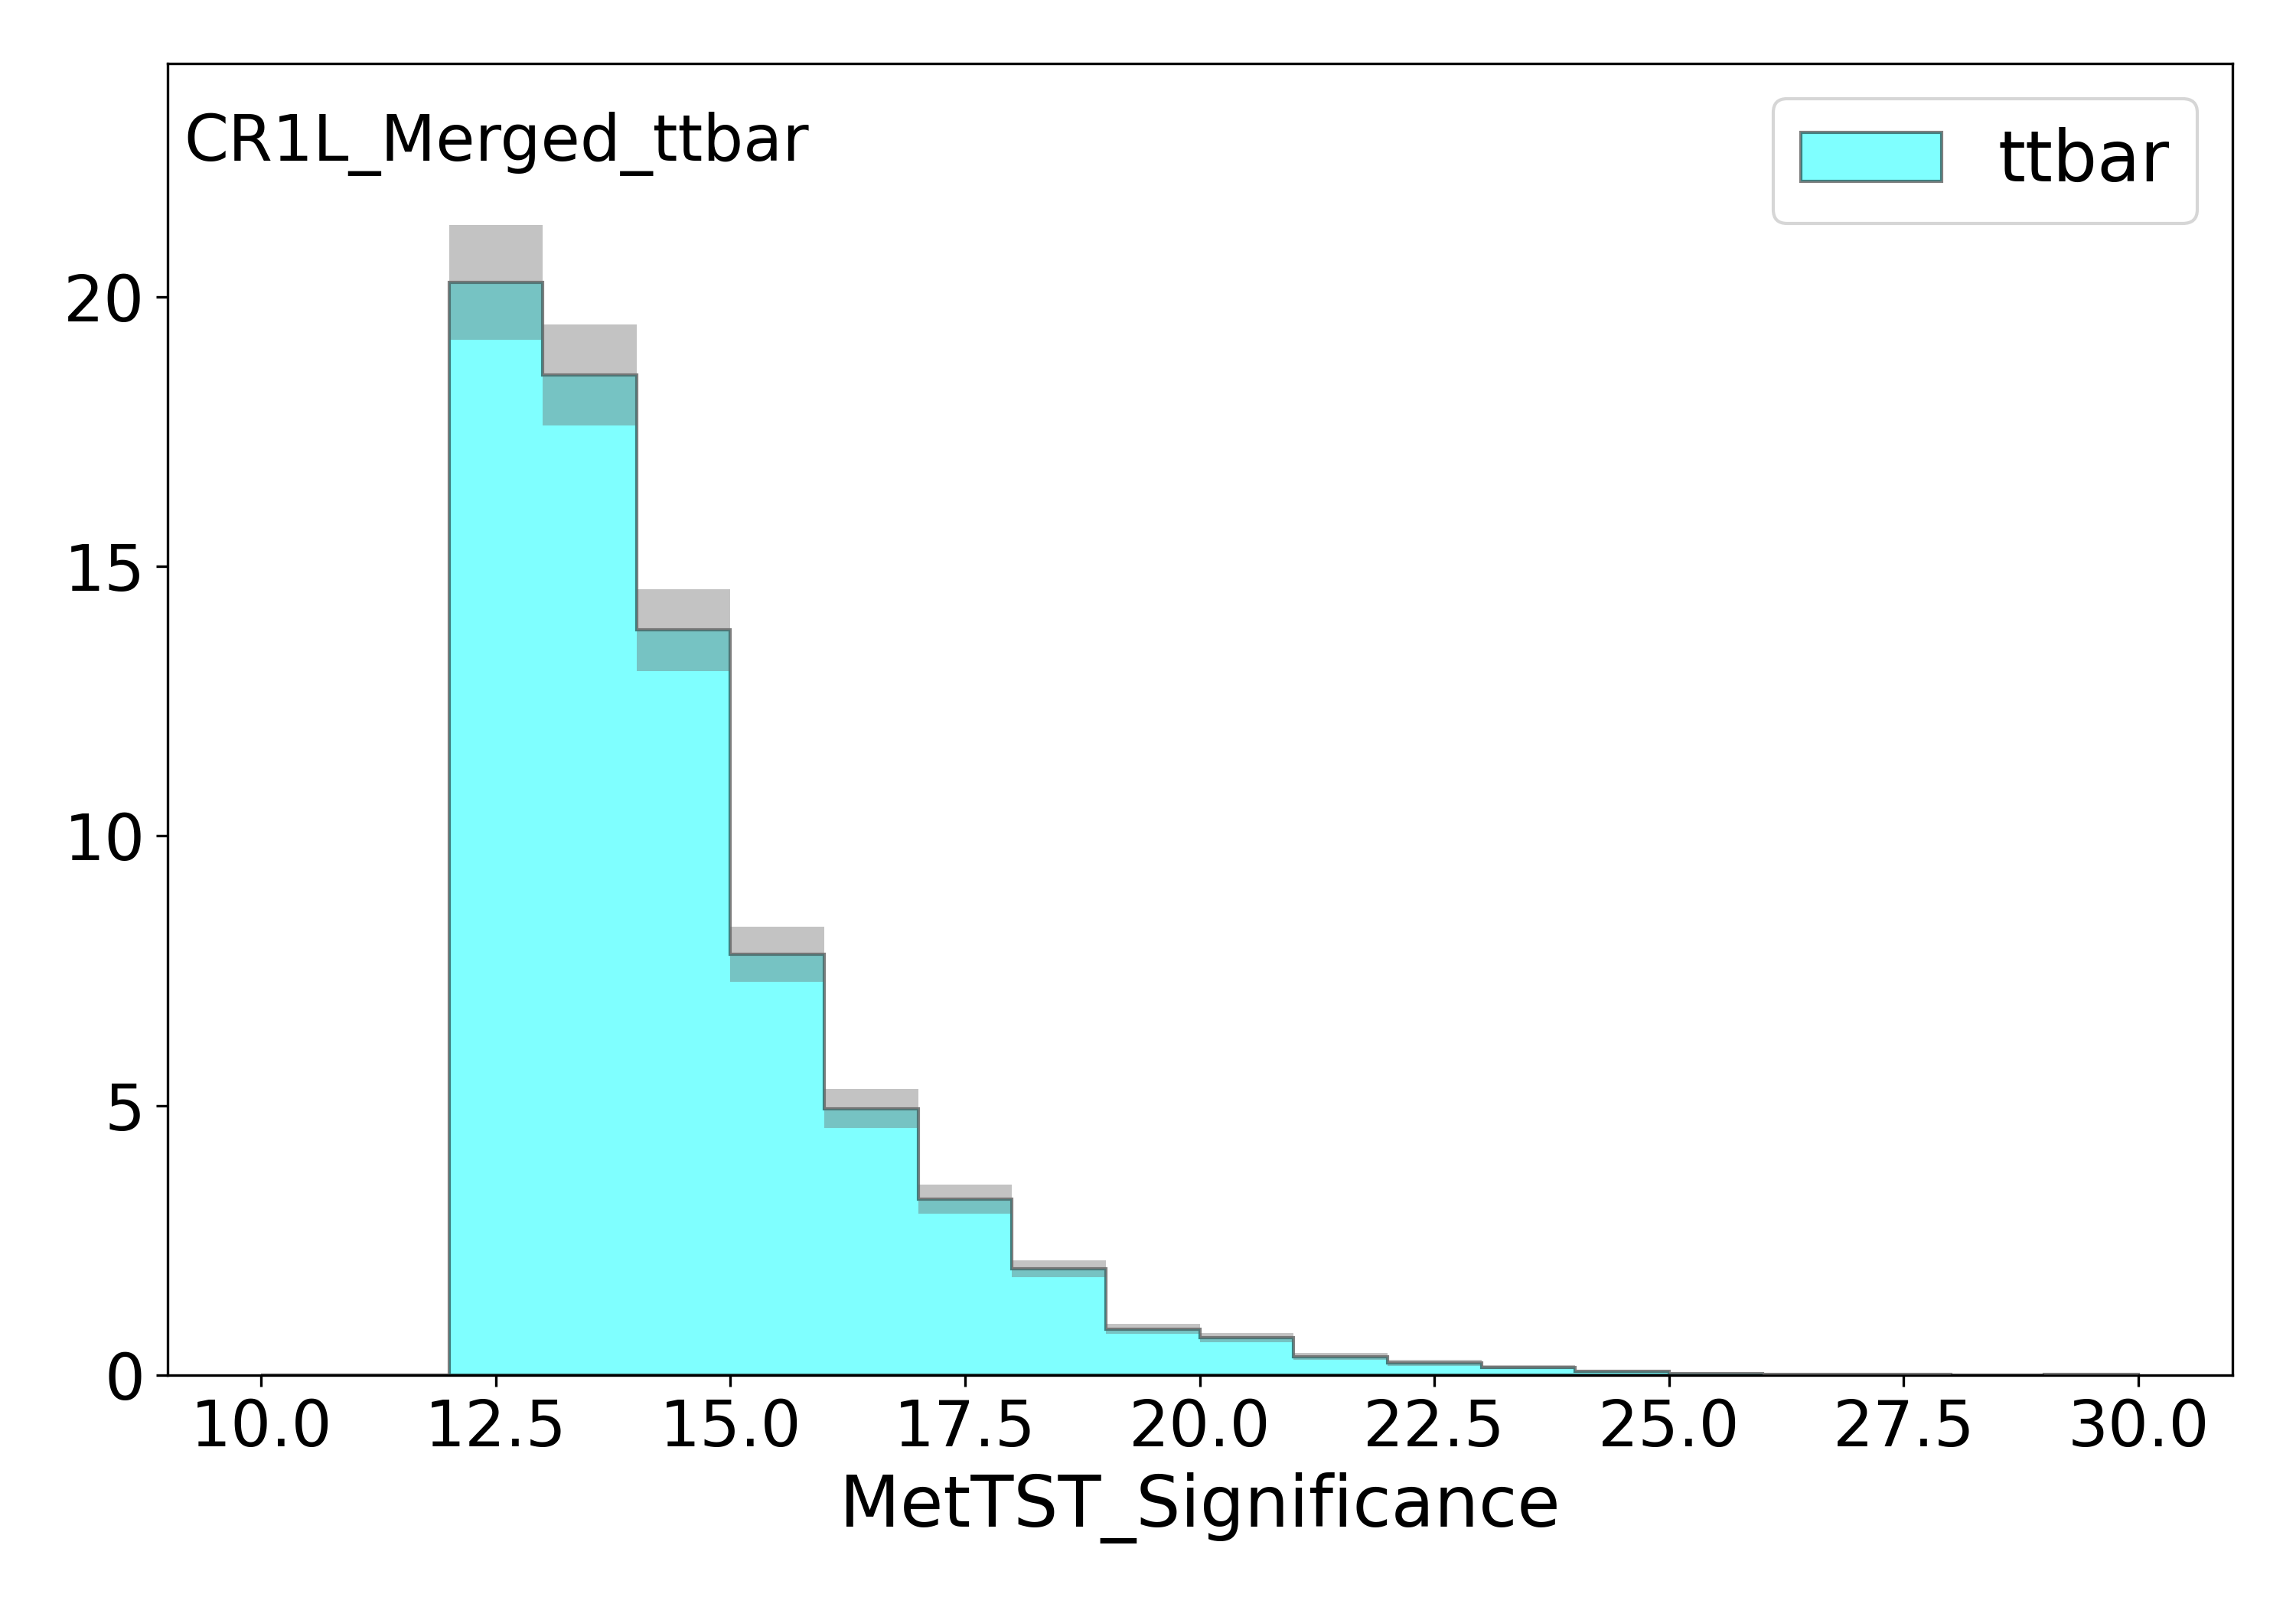
\includegraphics[width = 0.98\textwidth]{Figures/appendix/Preselection/MetTST_Significance.png}
     \caption{\metsig}
     \end{subfigure}
     \begin{subfigure}{0.49\textwidth}
     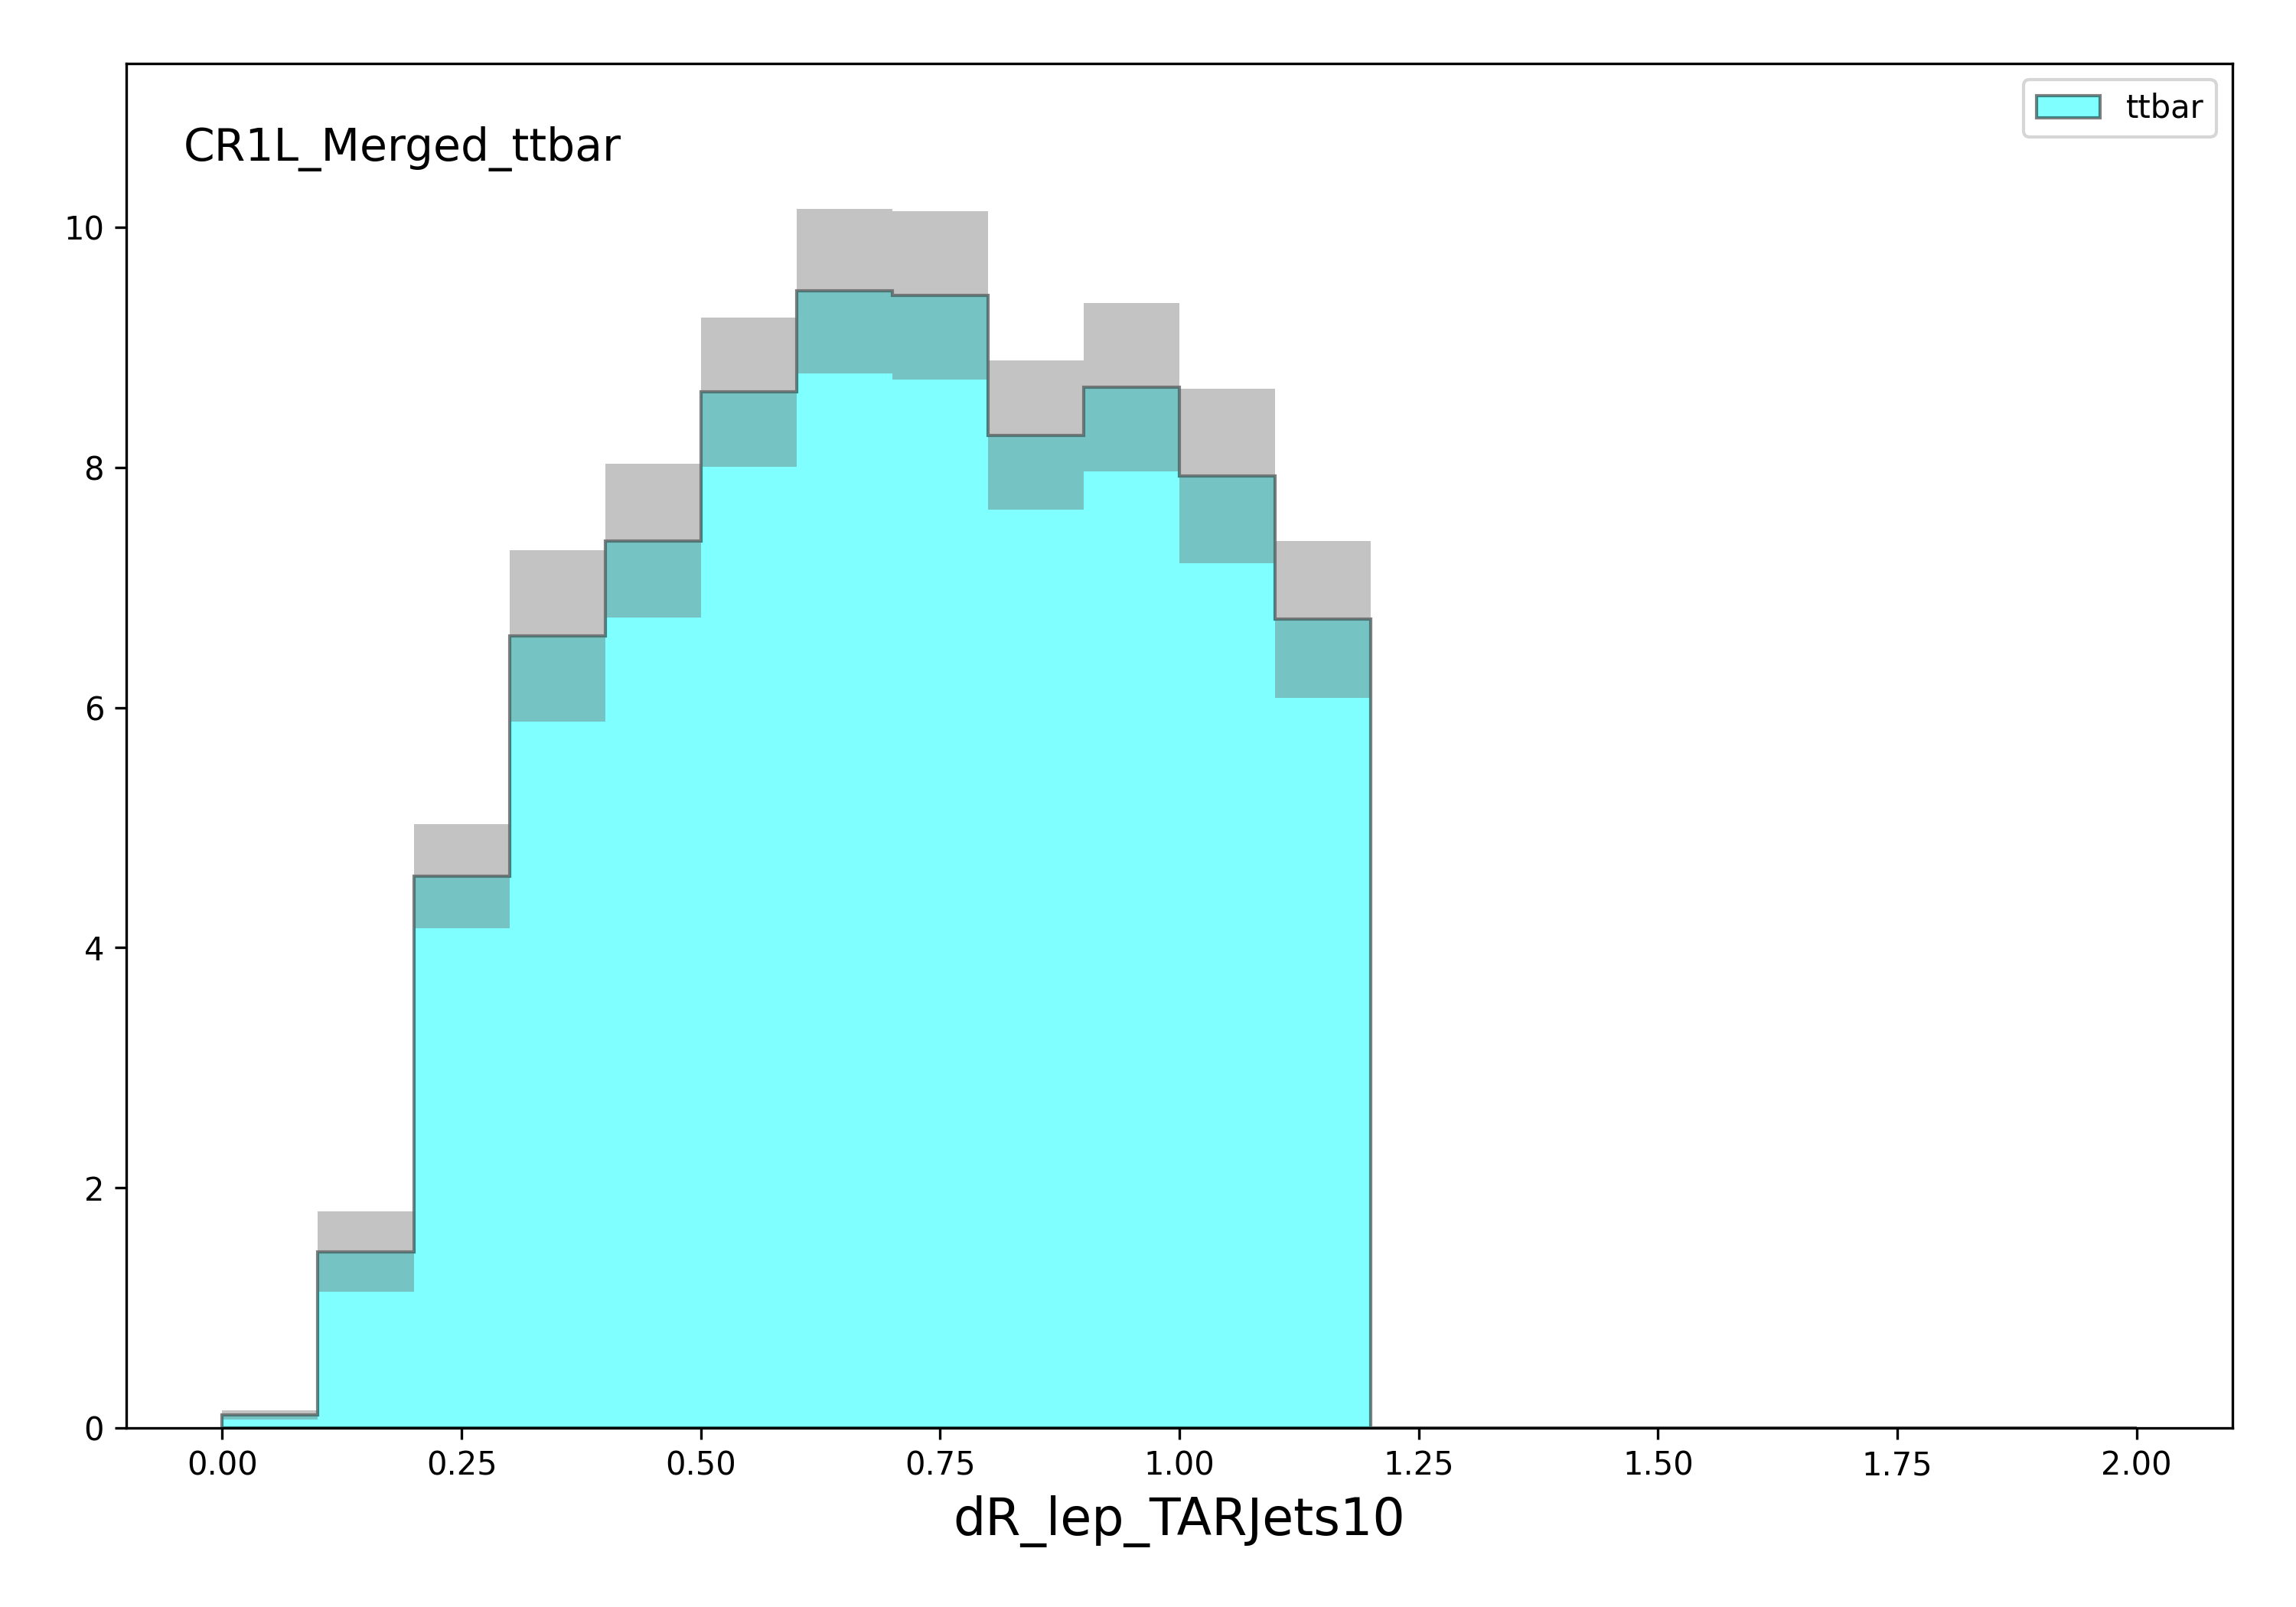
\includegraphics[width = 0.98\textwidth]{Figures/appendix/Preselection/dR_lep_TARJets10.png}
     \caption{\drTARl}
     \end{subfigure}
     \begin{subfigure}{0.49\textwidth}
     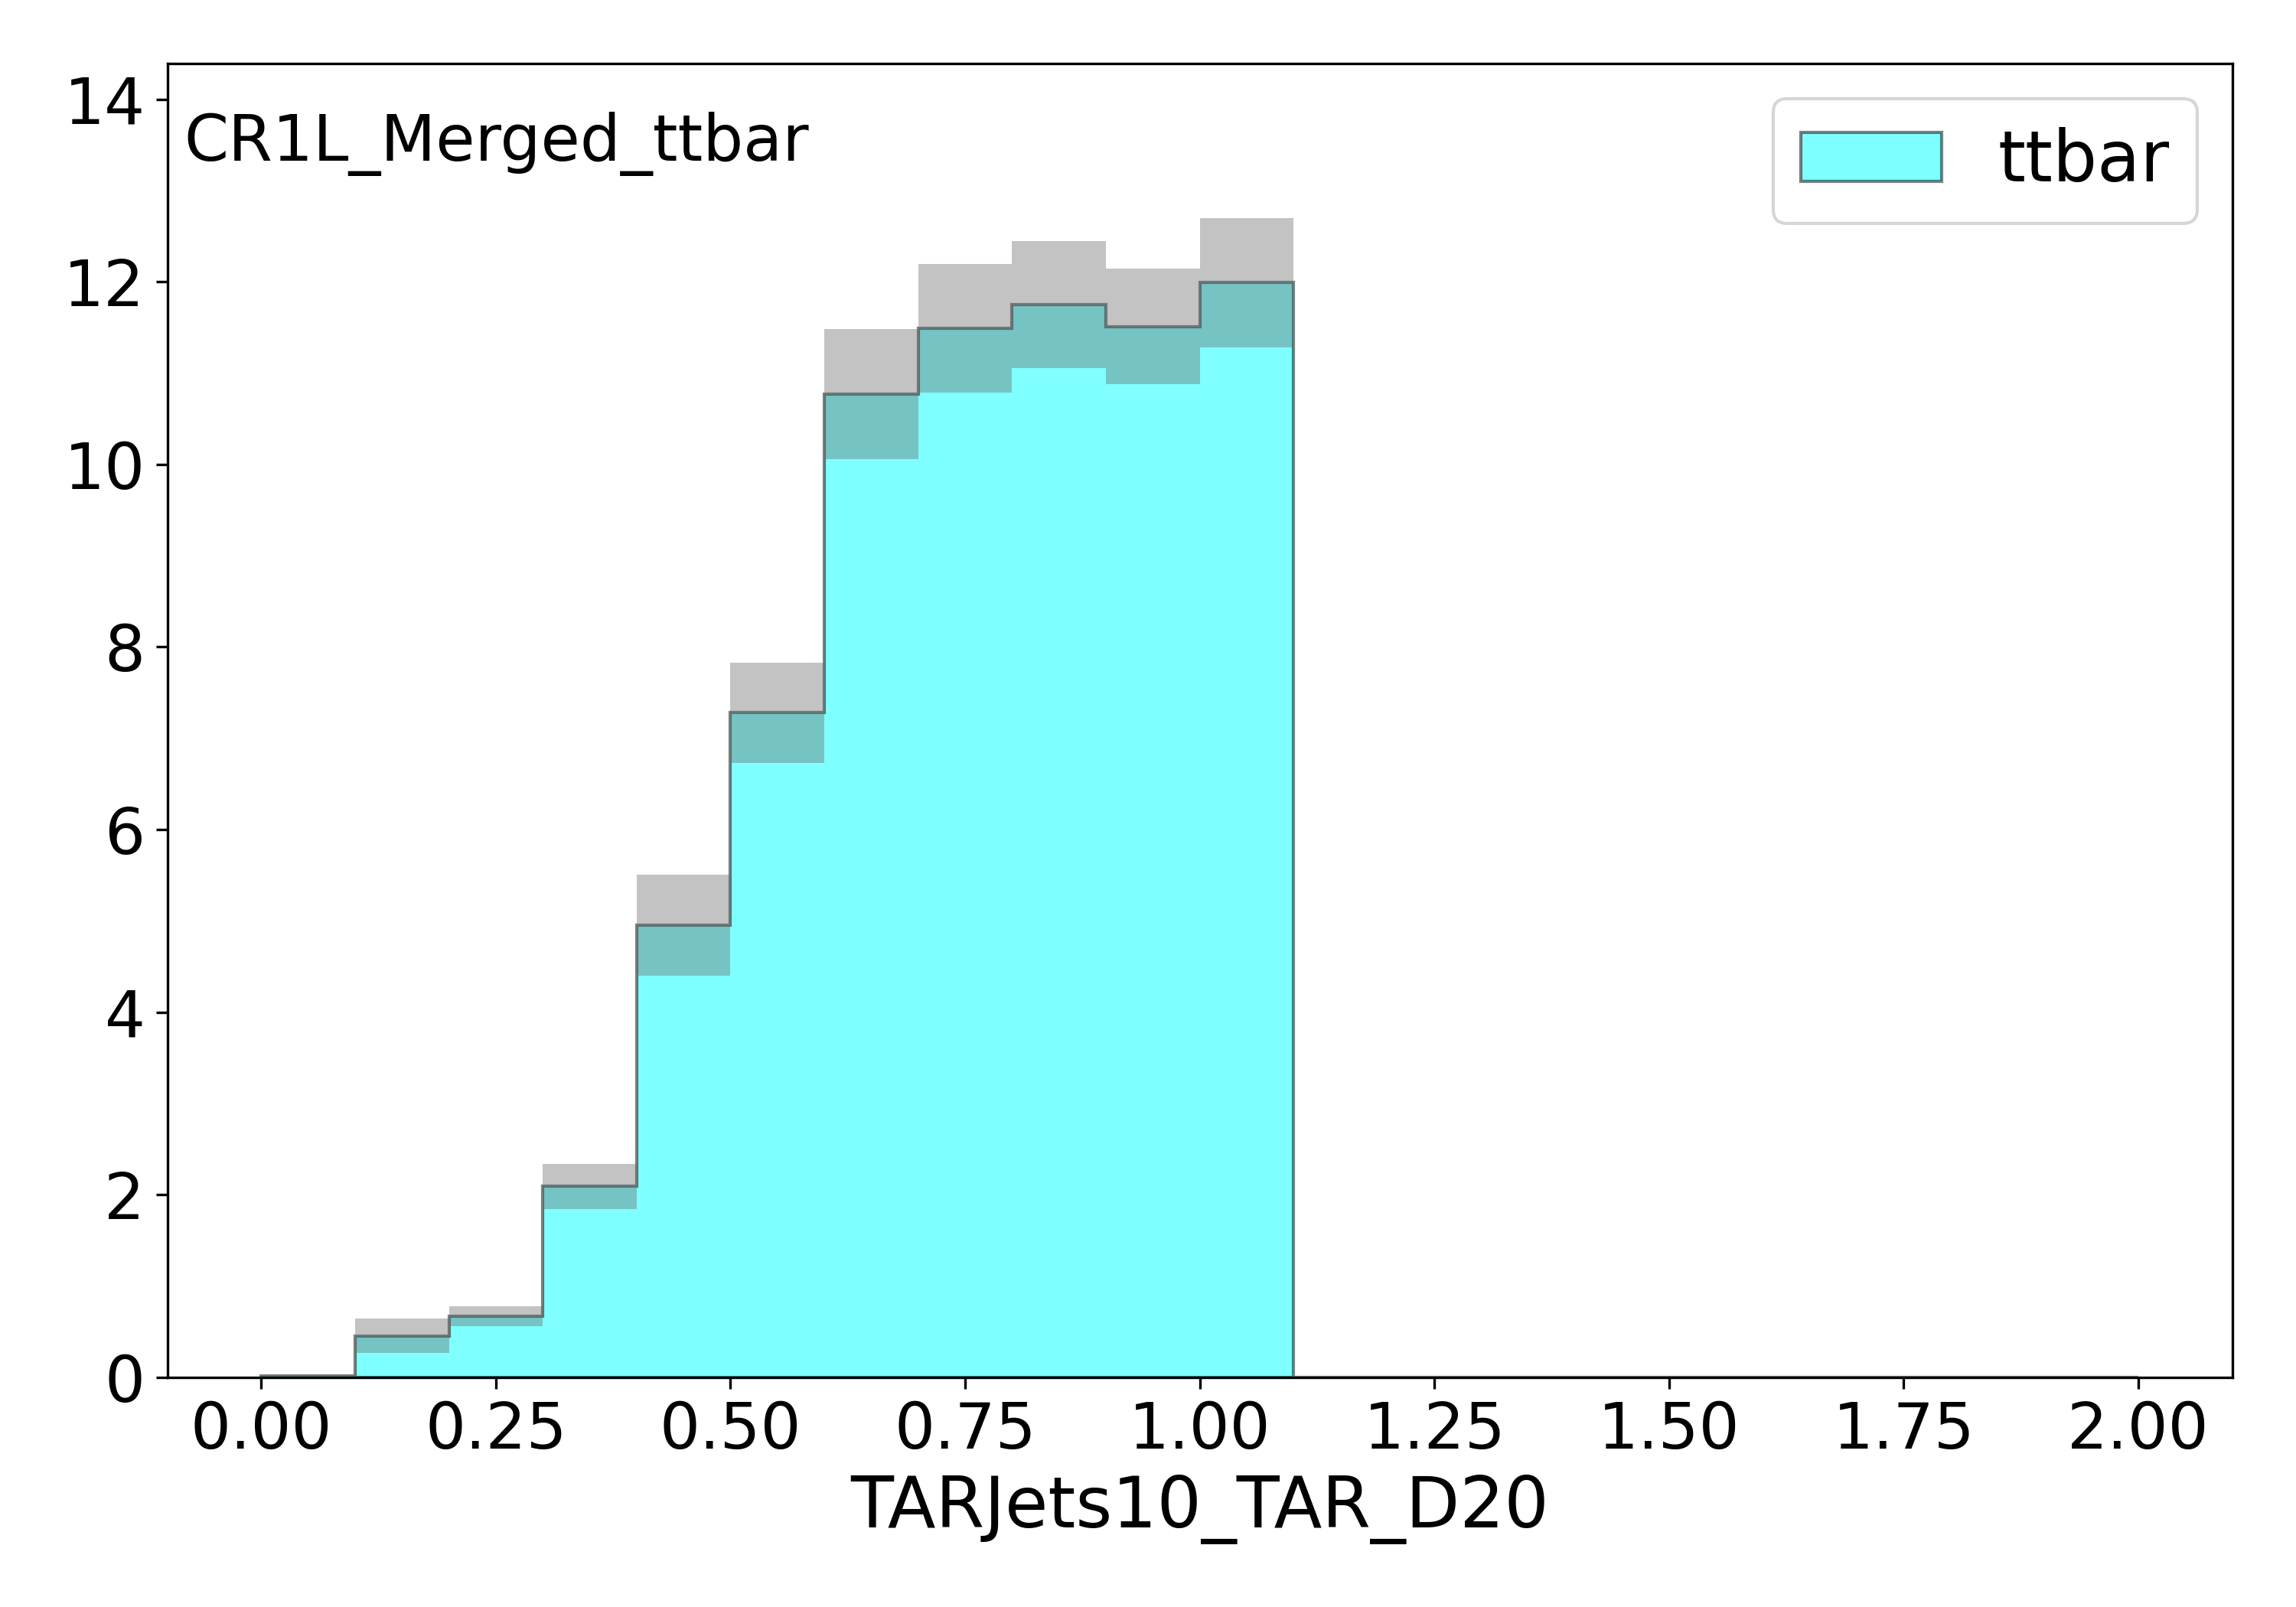
\includegraphics[width = 0.98\textwidth]{Figures/appendix/Preselection/TARJets10_TAR_D20.png}
     \caption{\DtwoTAR}
     \end{subfigure}
     \begin{subfigure}{0.49\textwidth}
     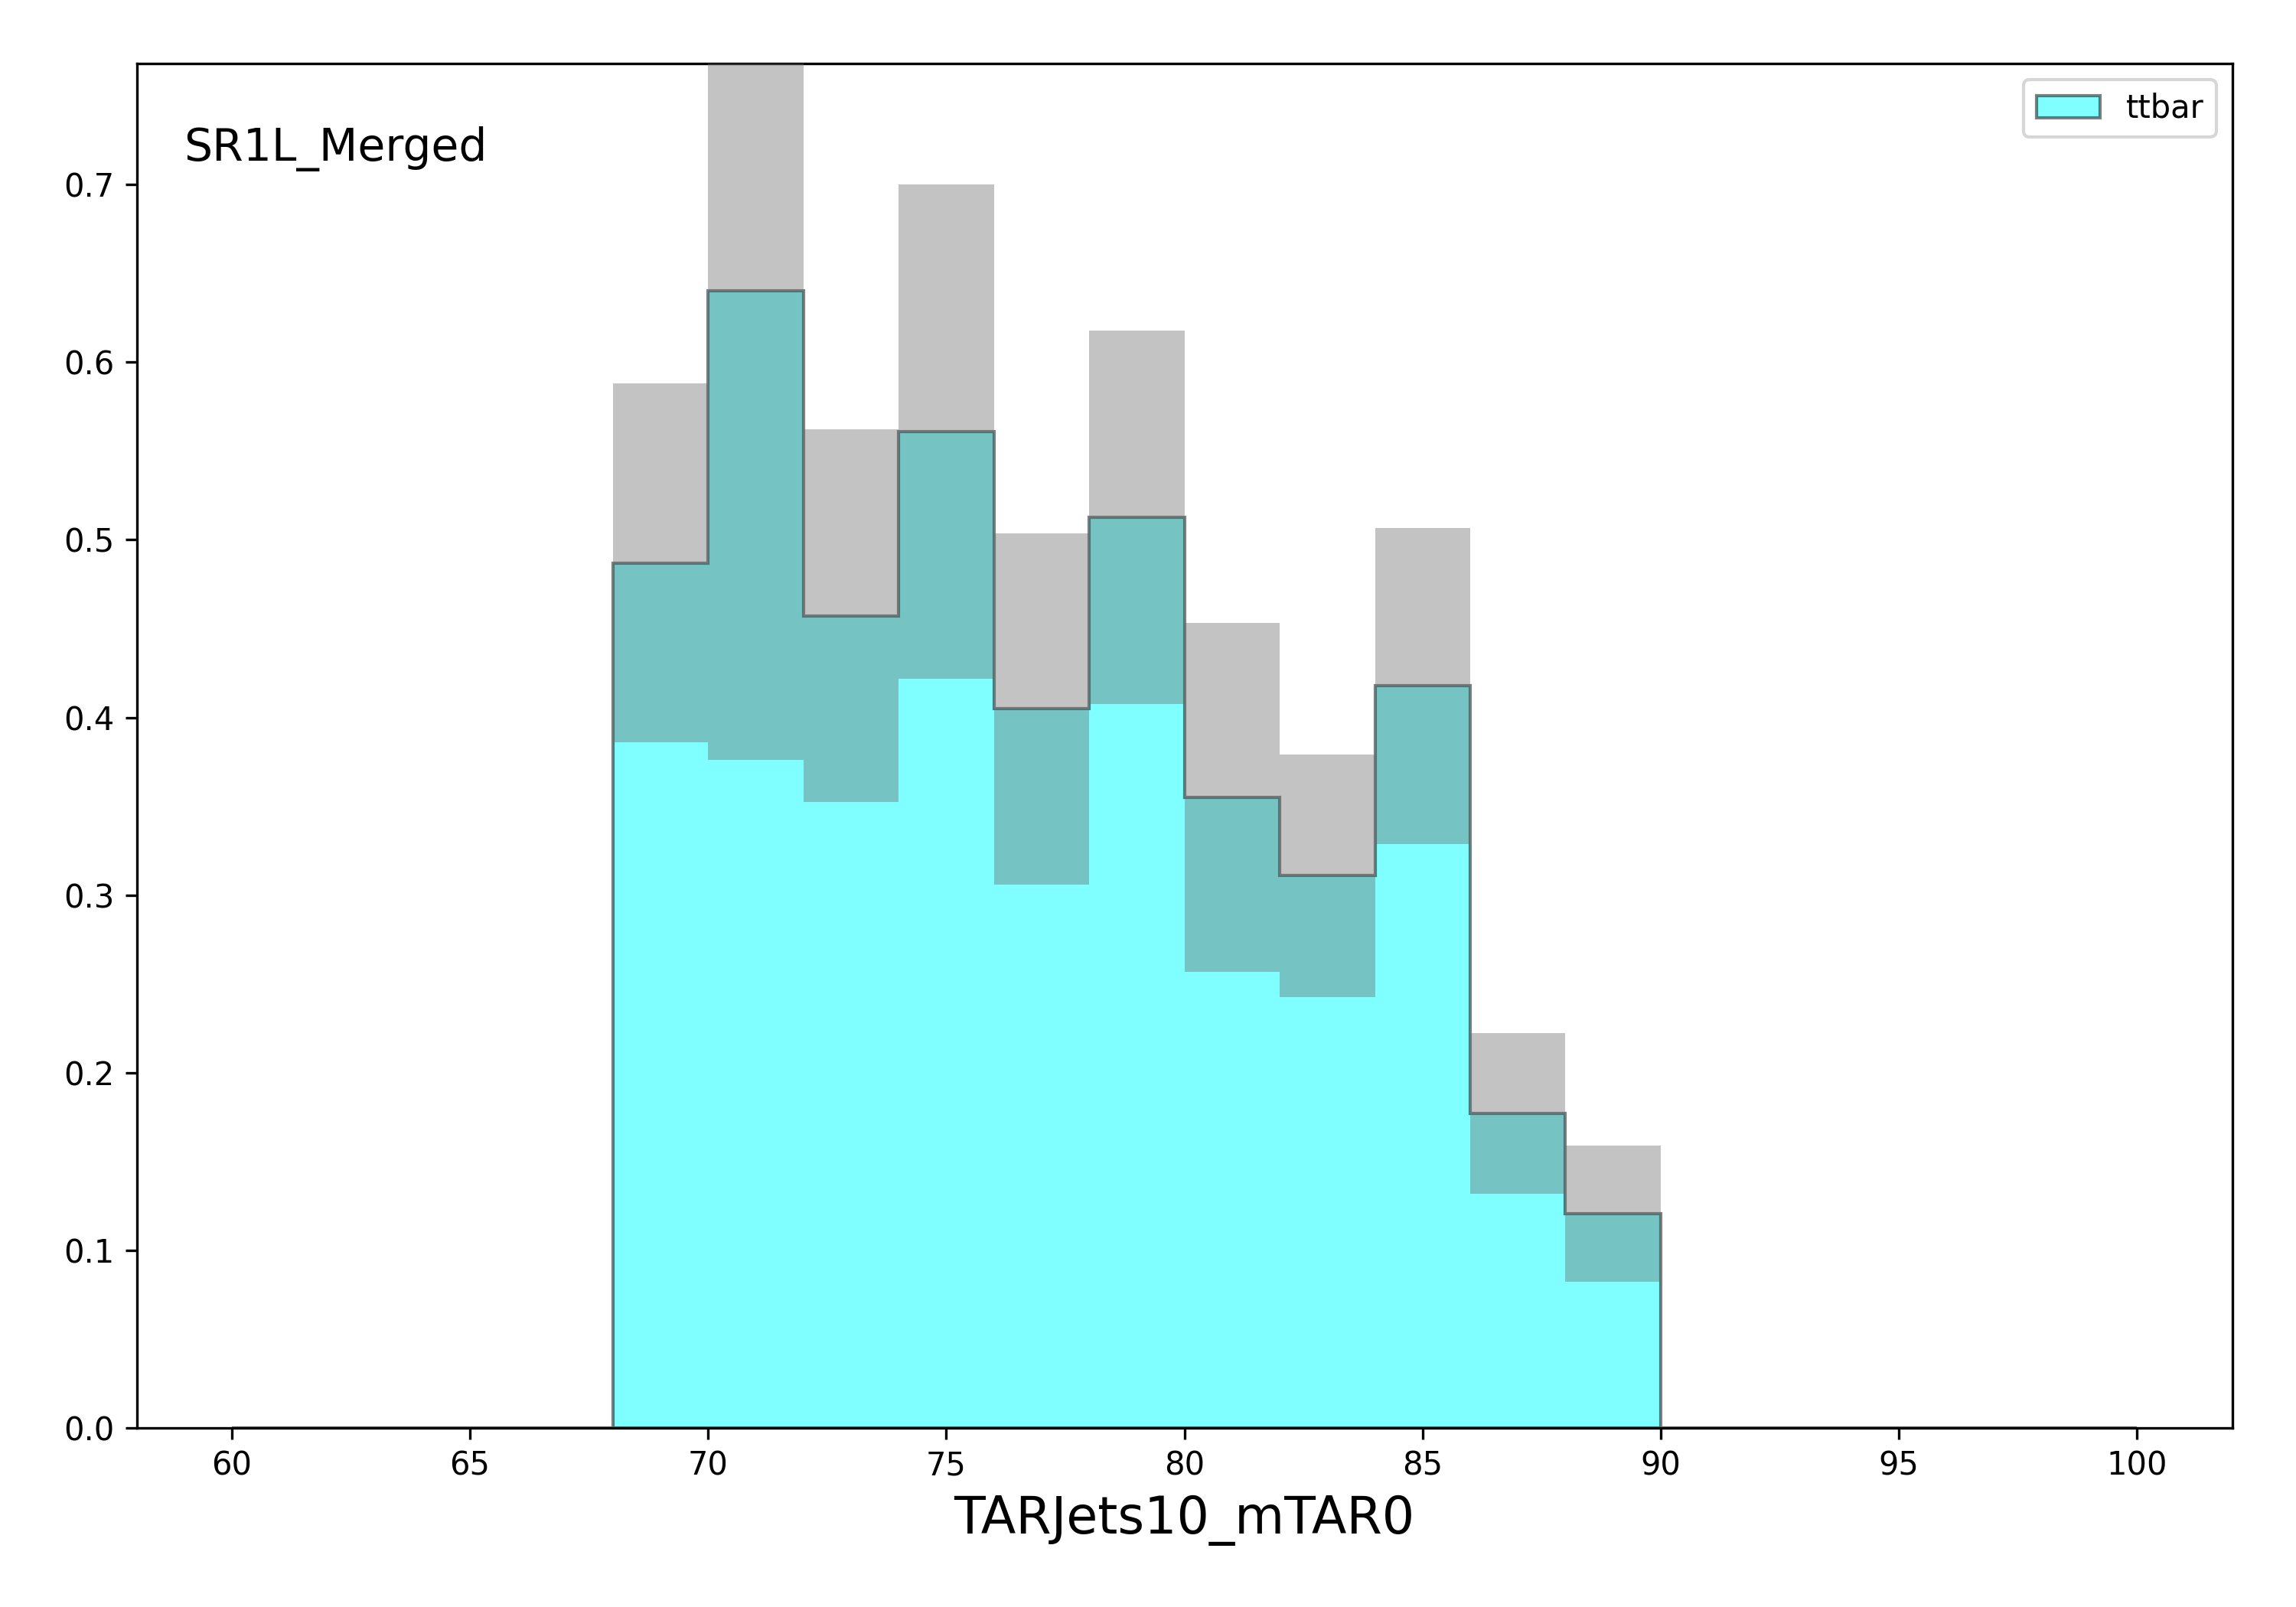
\includegraphics[width = 0.98\textwidth]{Figures/appendix/Preselection/TARJets10_mTAR0.png}
     \caption{\mTAR}
     \end{subfigure}
     \begin{subfigure}{0.49\textwidth}
     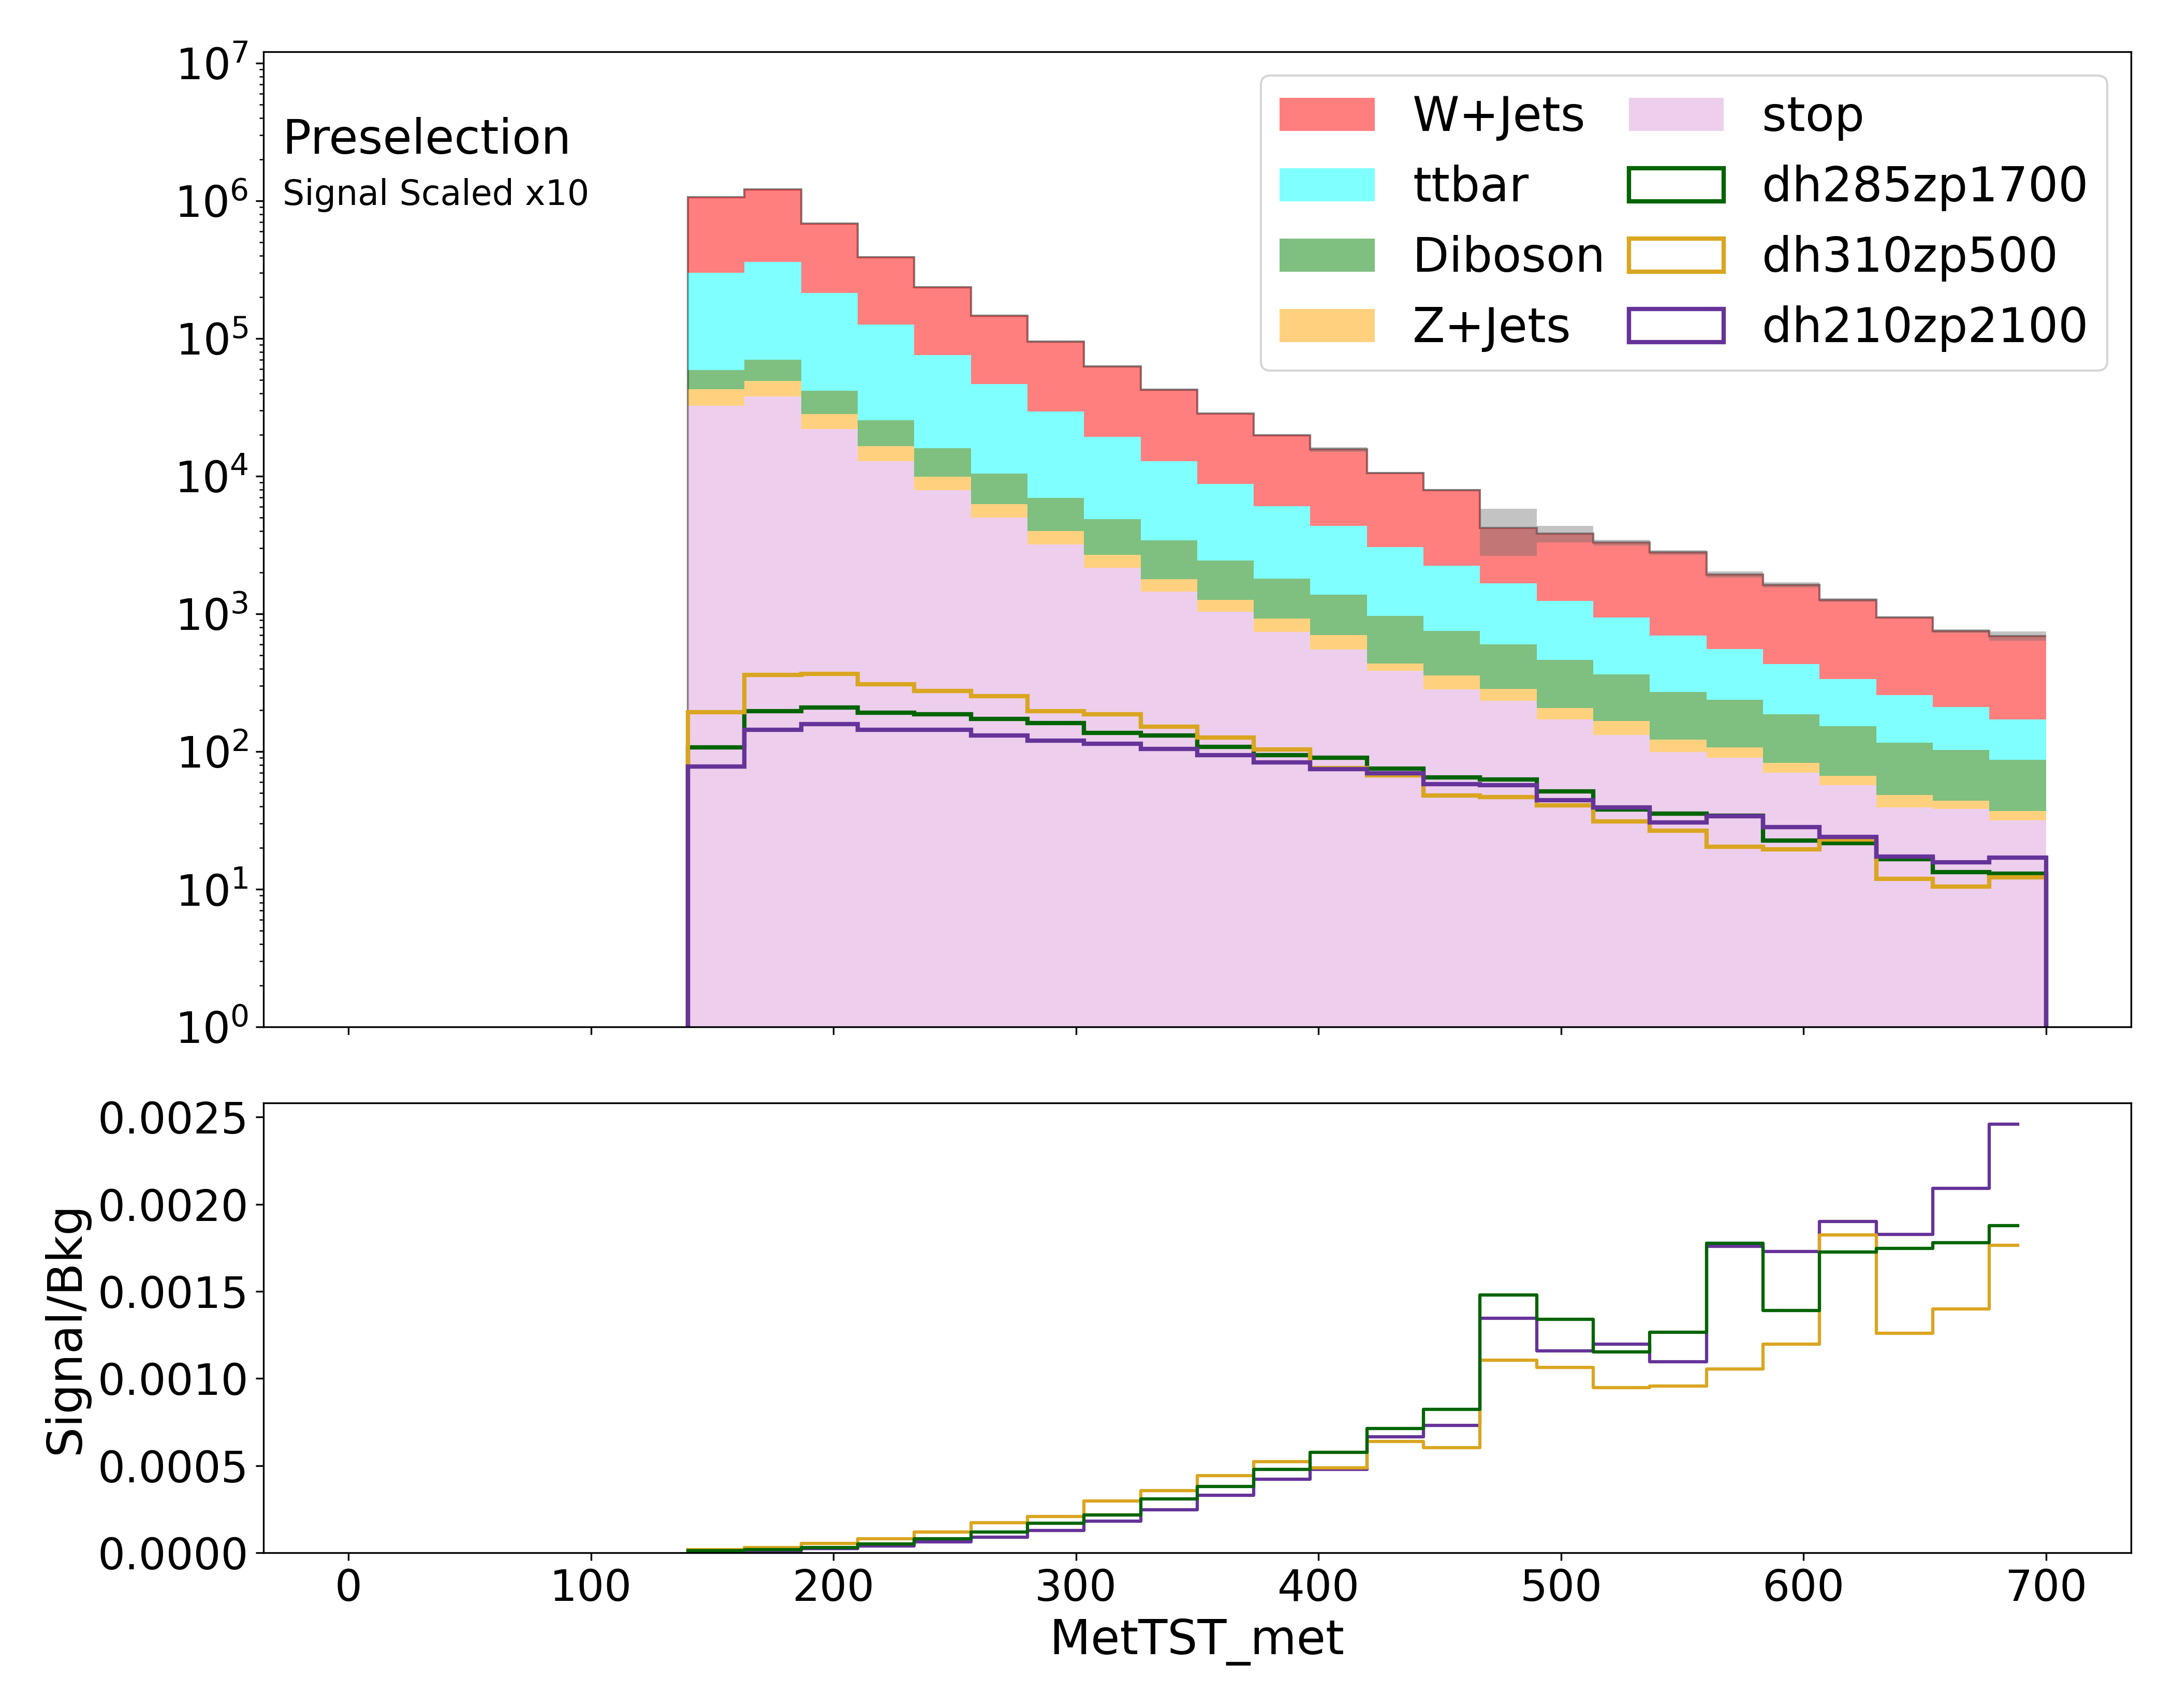
\includegraphics[width = 0.98\textwidth]{Figures/appendix/Preselection/MetTST_met.png}
     \caption{\met}
     \end{subfigure}

     \caption{Preselection level distribuitions.}
     \label{fig:Presel1}
  \end{figure}

  \begin{figure}[htbp]
    \centering
      \begin{subfigure}{0.49\textwidth}
      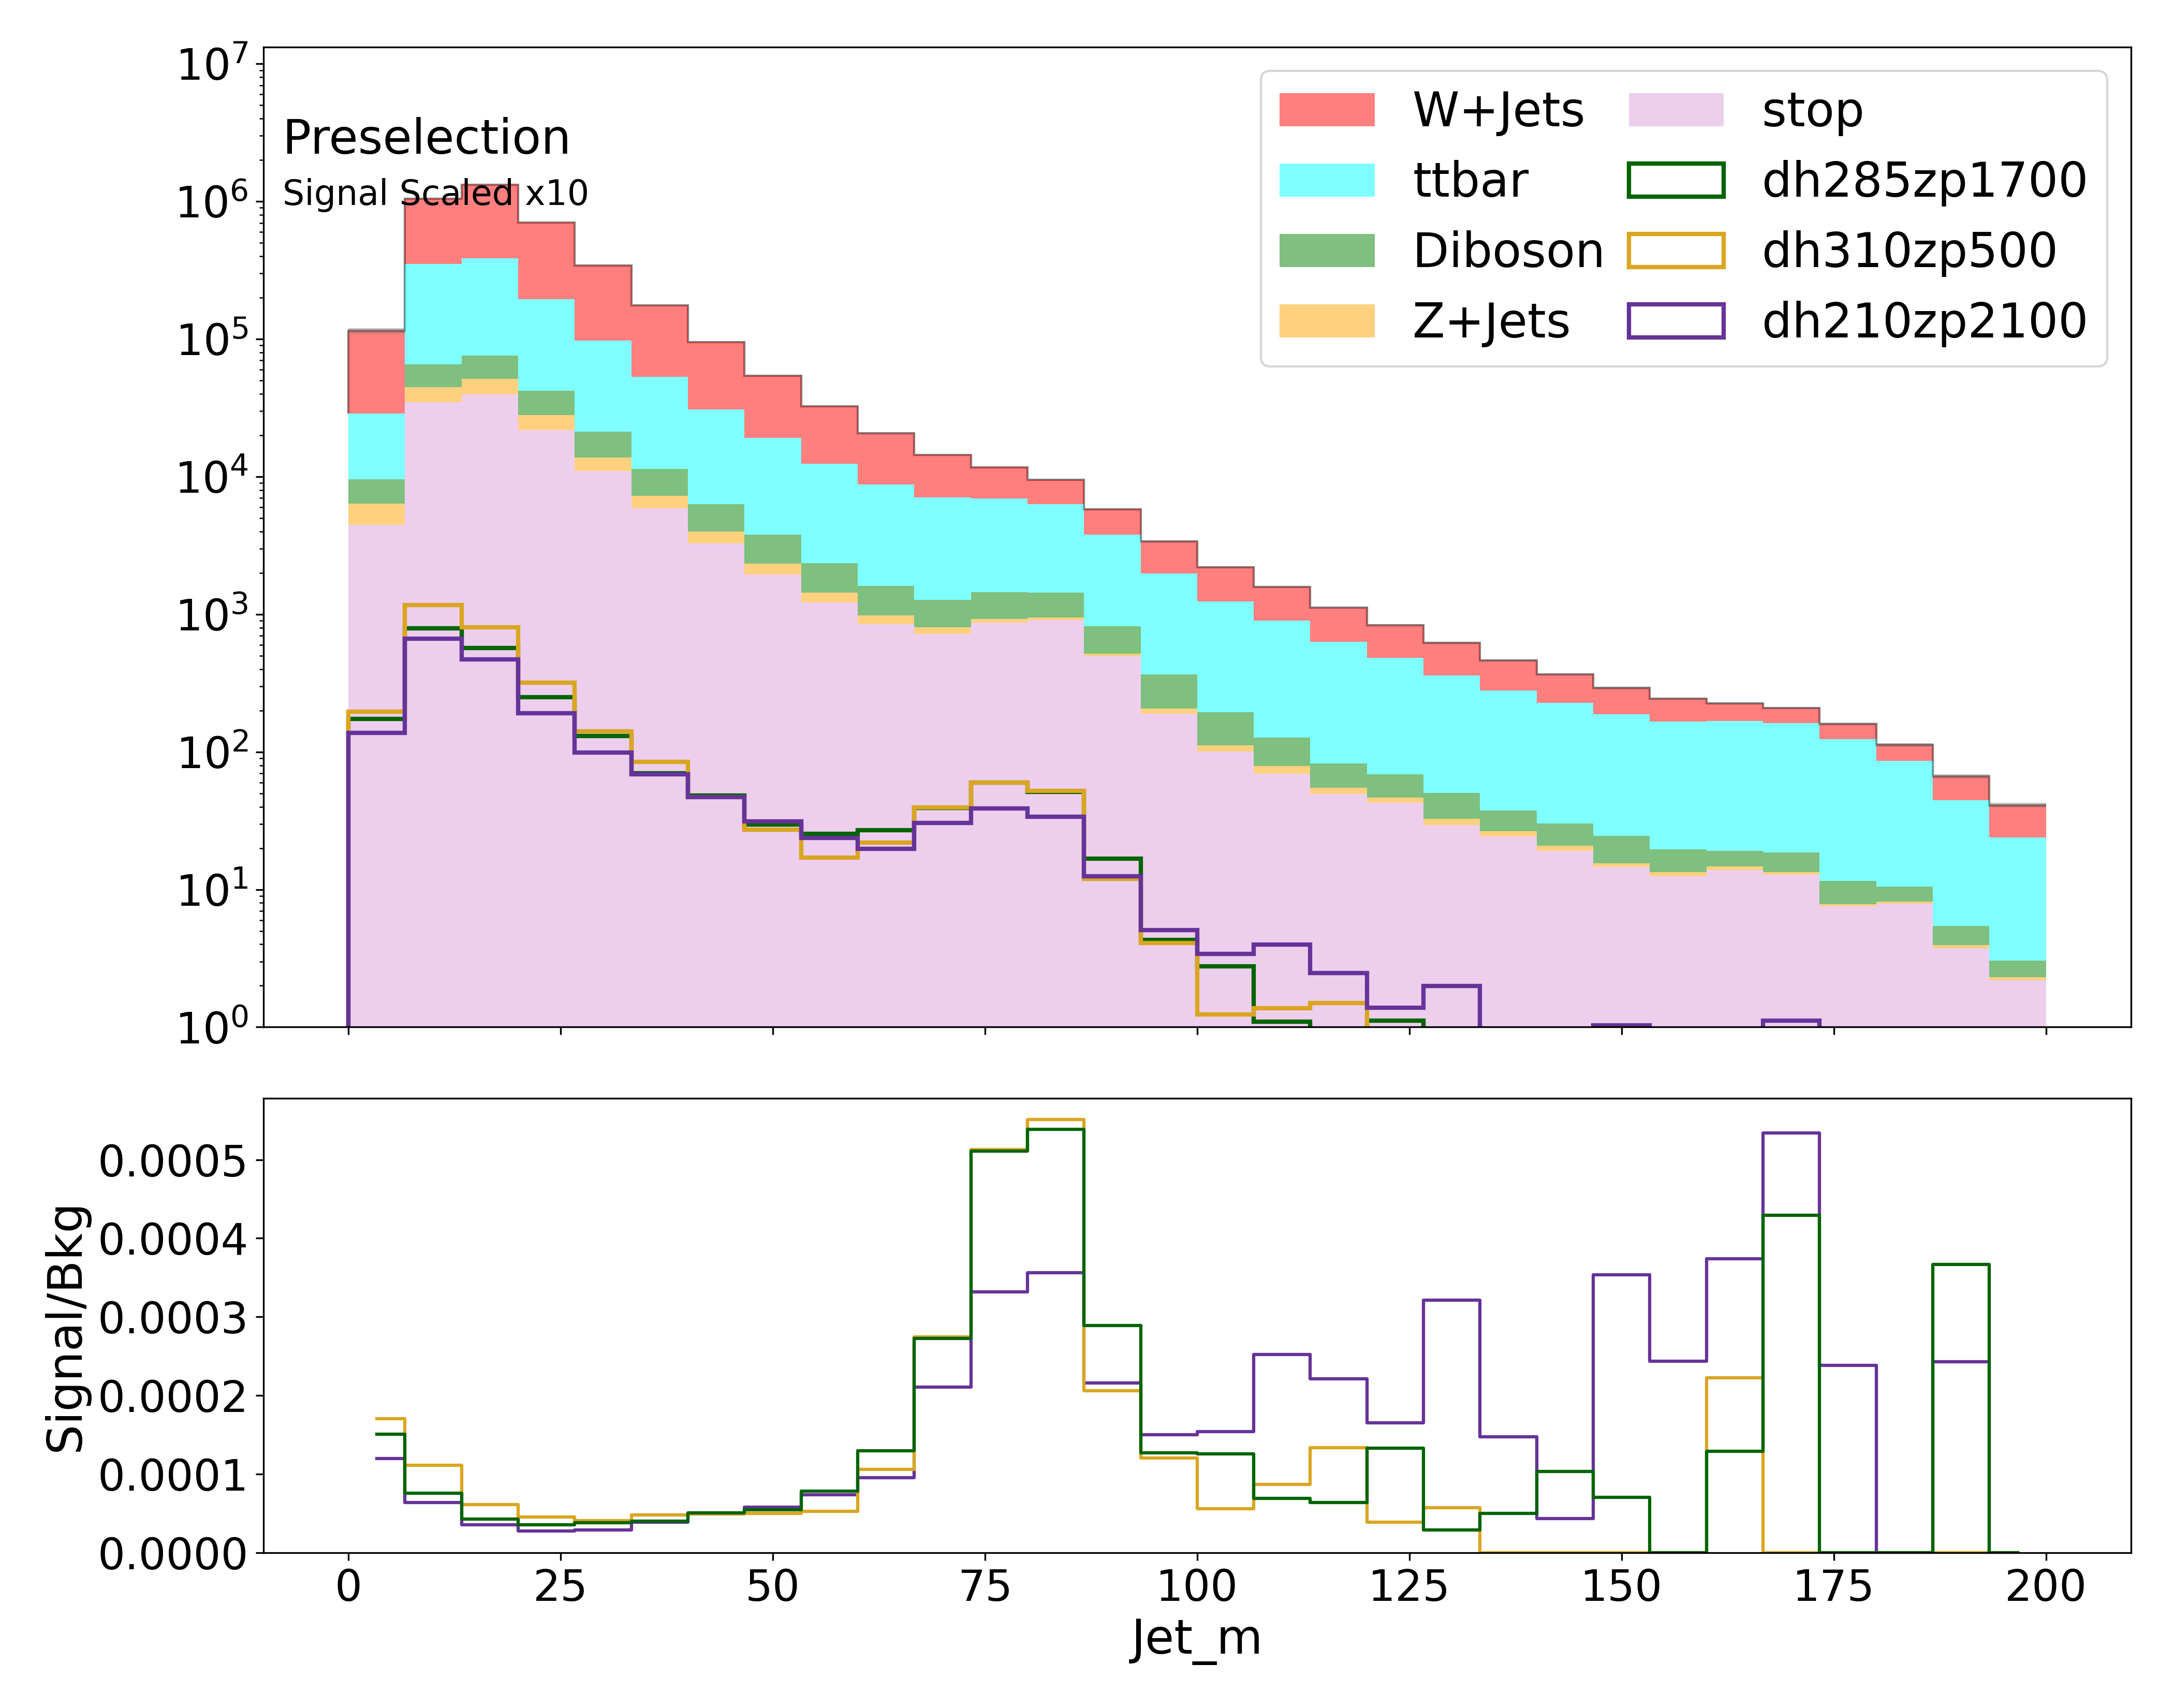
\includegraphics[width = 0.98\textwidth]{Figures/appendix/Preselection/Jet_m.png}
      \caption{\ensuremath{m_{\text{Jet}}}}
      \end{subfigure}
      \begin{subfigure}{0.49\textwidth}
      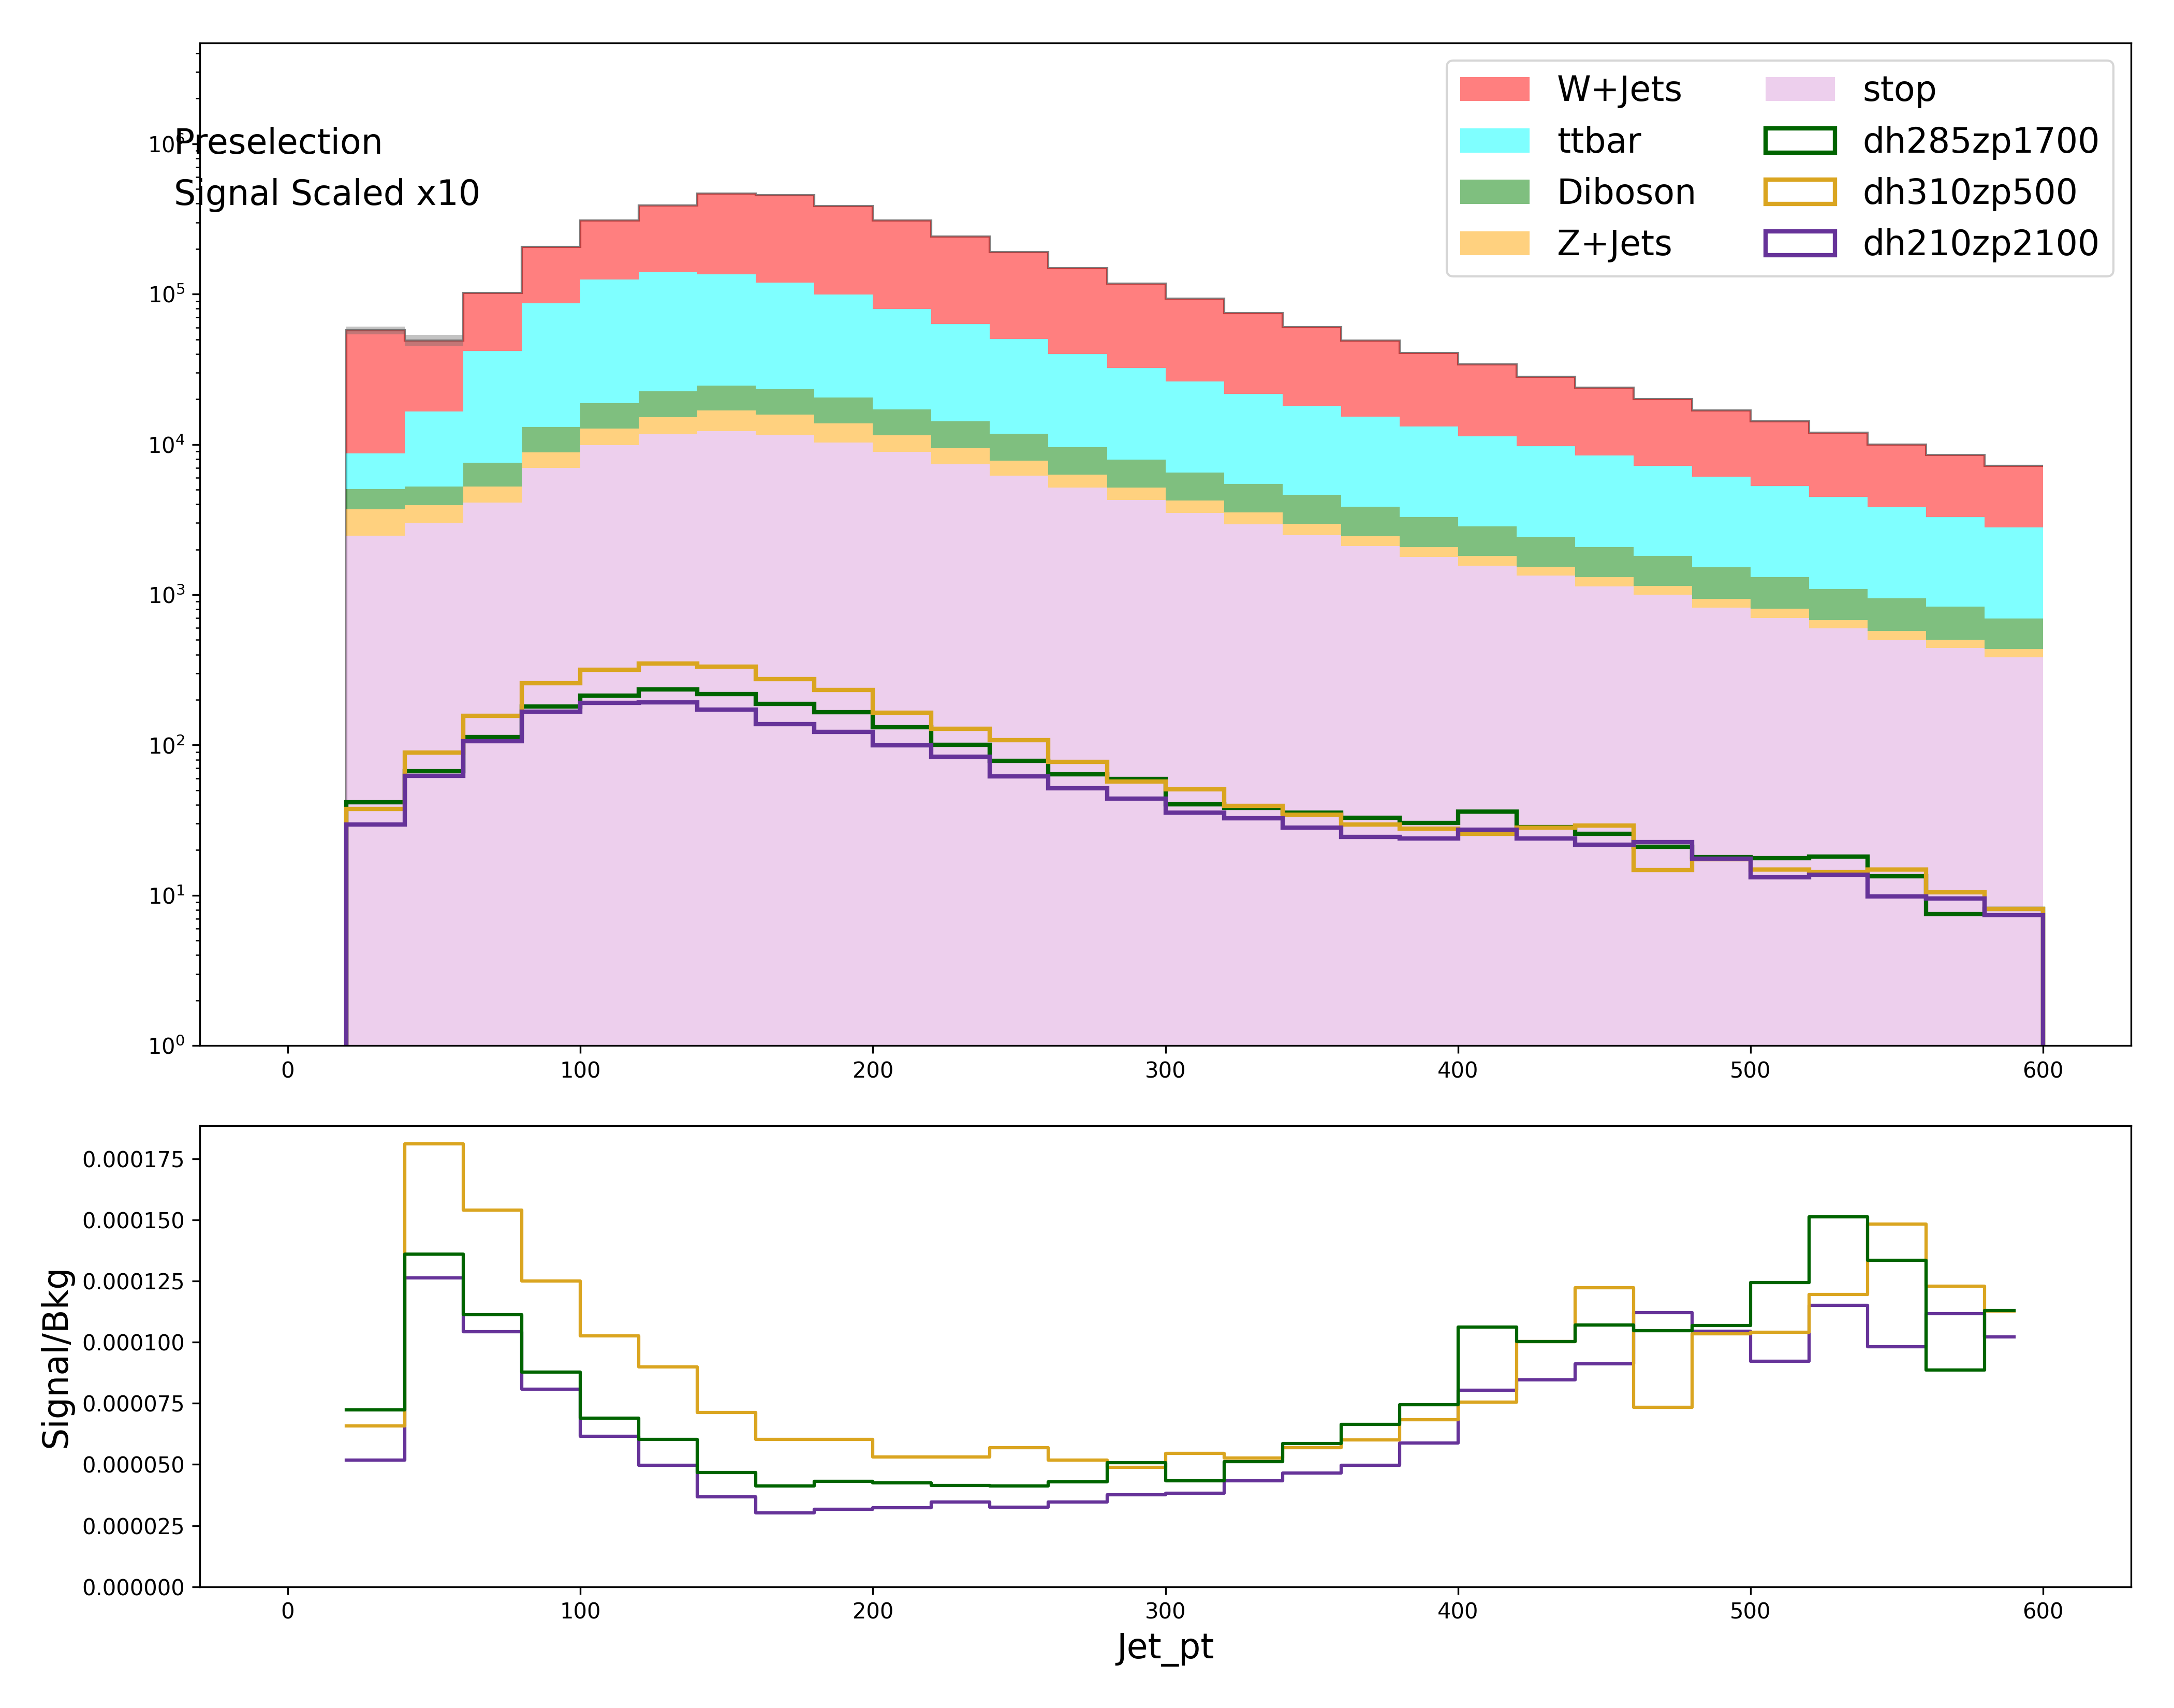
\includegraphics[width = 0.98\textwidth]{Figures/appendix/Preselection/Jet_pt.png}
      \caption{\ensuremath{\pT(\text{Jet})}}
      \end{subfigure}
      \begin{subfigure}{0.49\textwidth}
      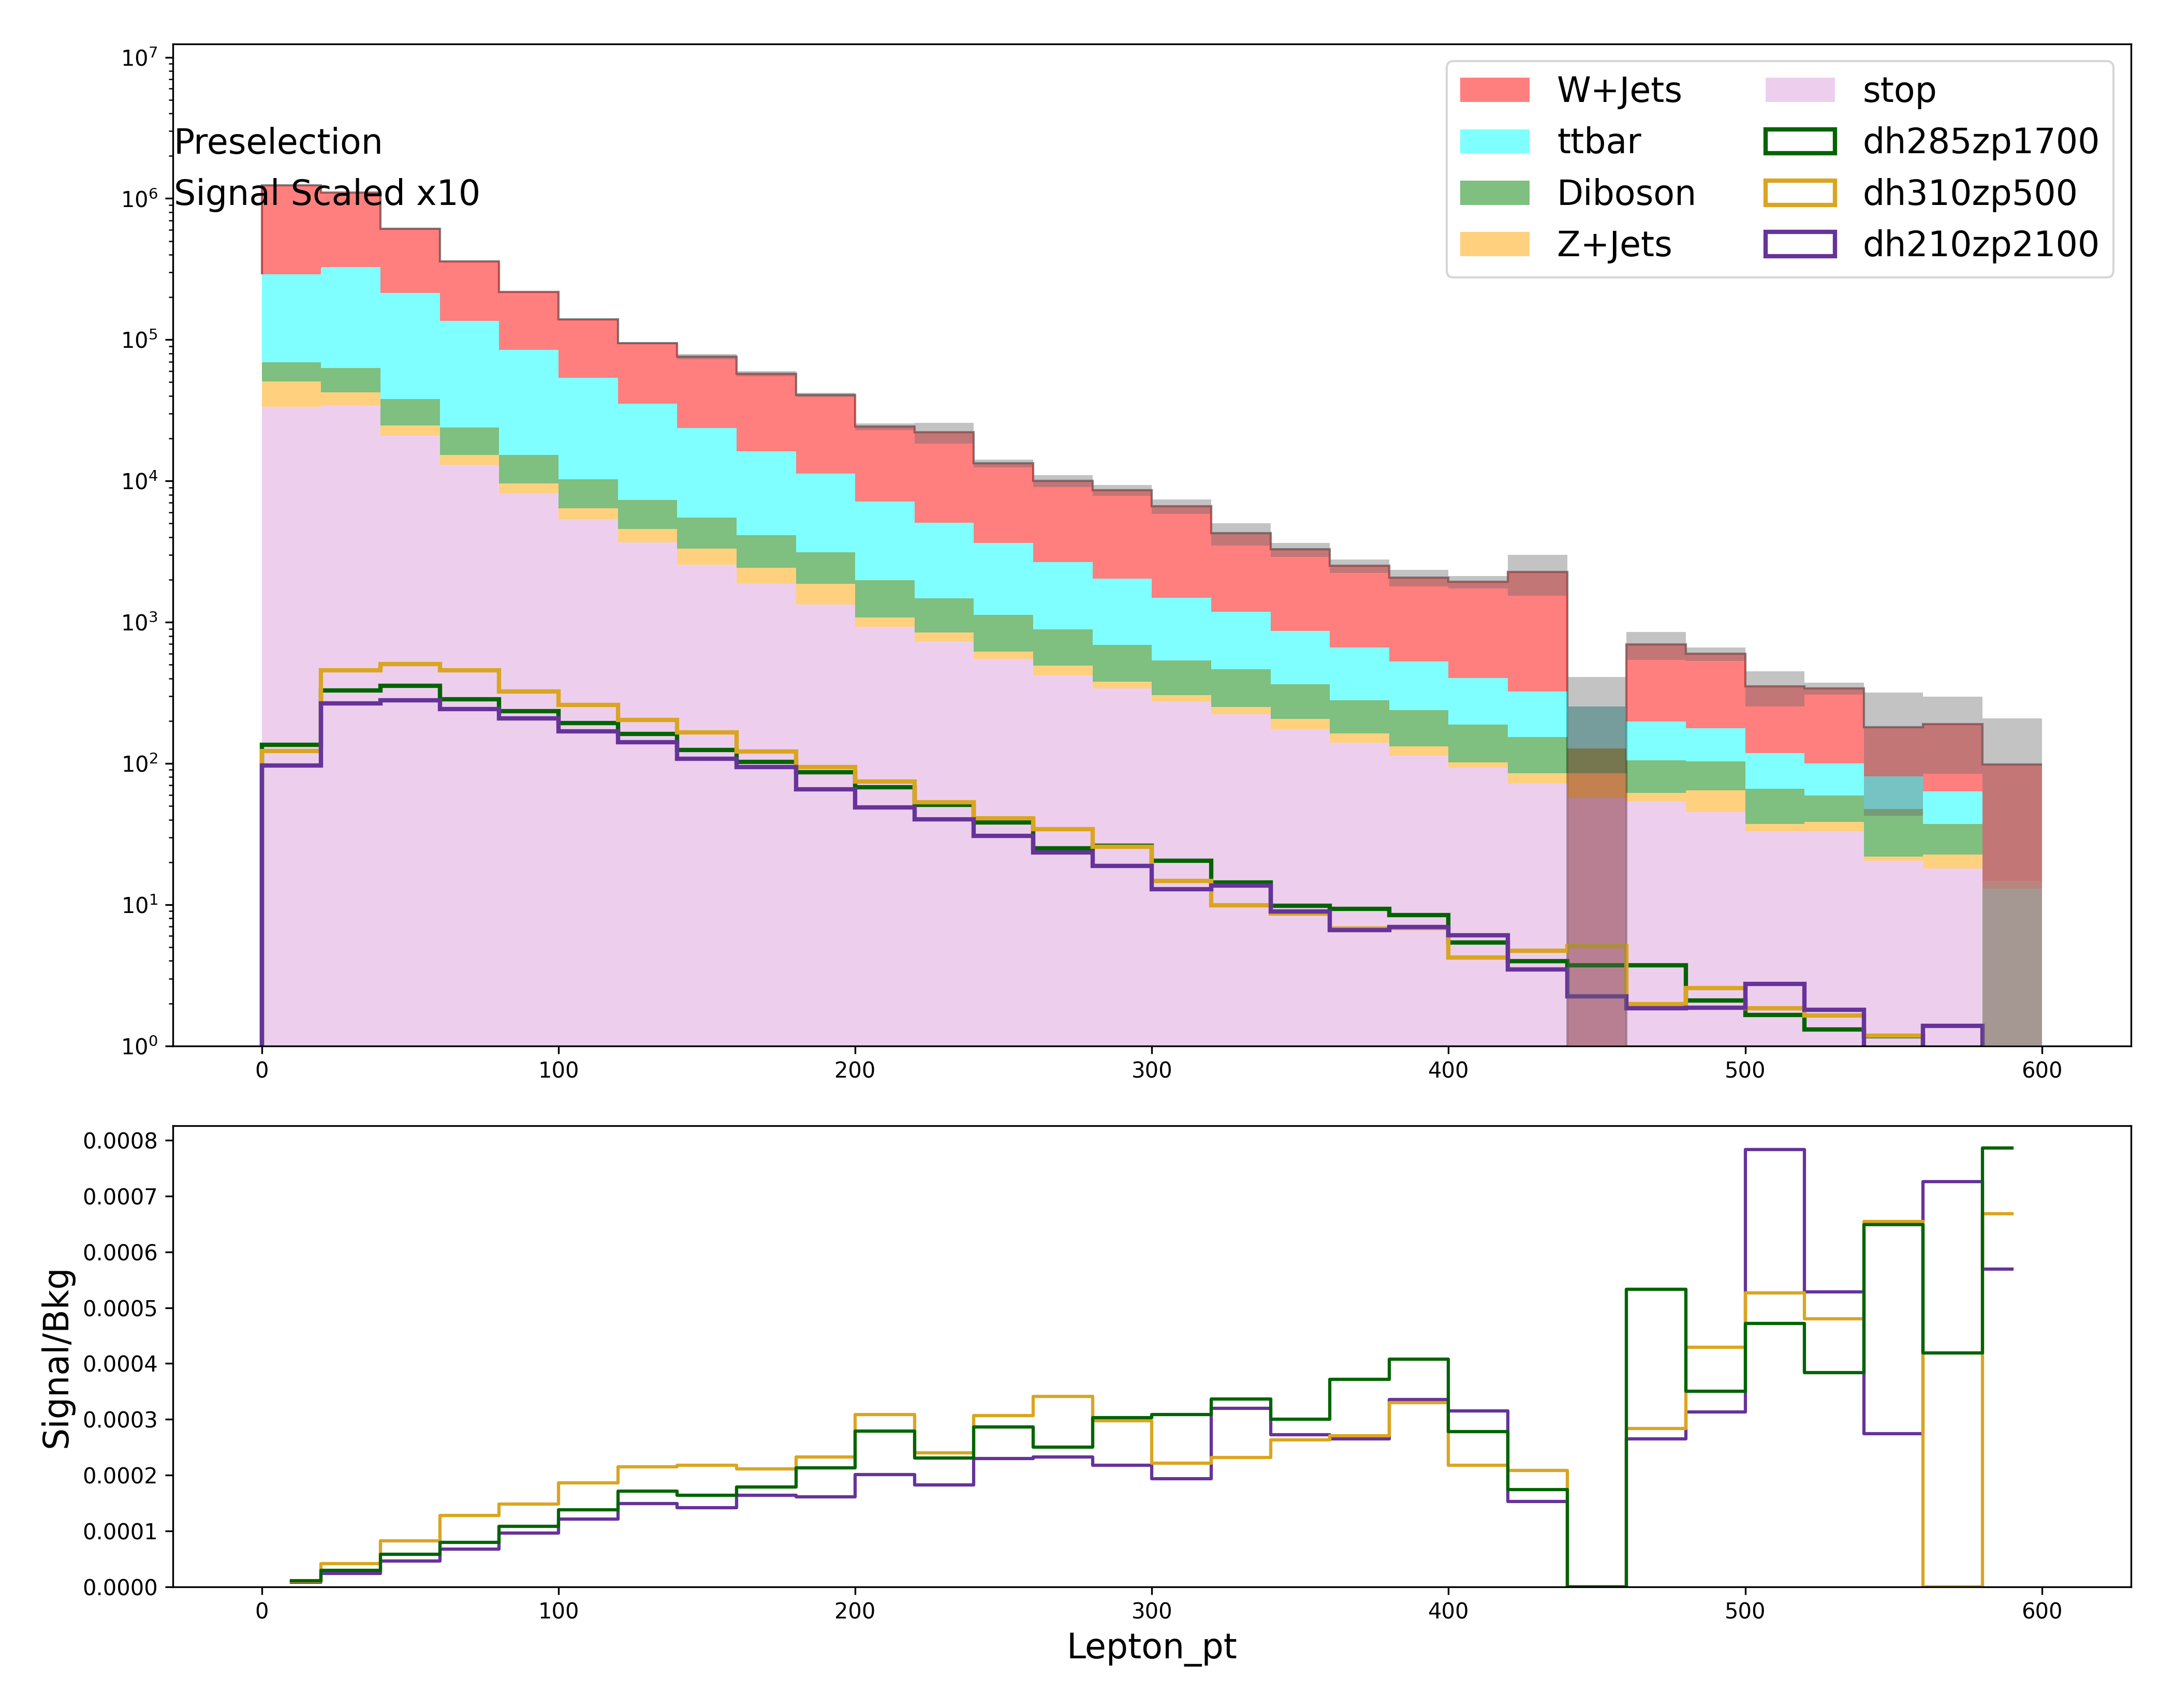
\includegraphics[width = 0.98\textwidth]{Figures/appendix/Preselection/Lepton_pt.png}
      \caption{$\pT(\ell)$}
      \end{subfigure}
      \begin{subfigure}{0.49\textwidth}
      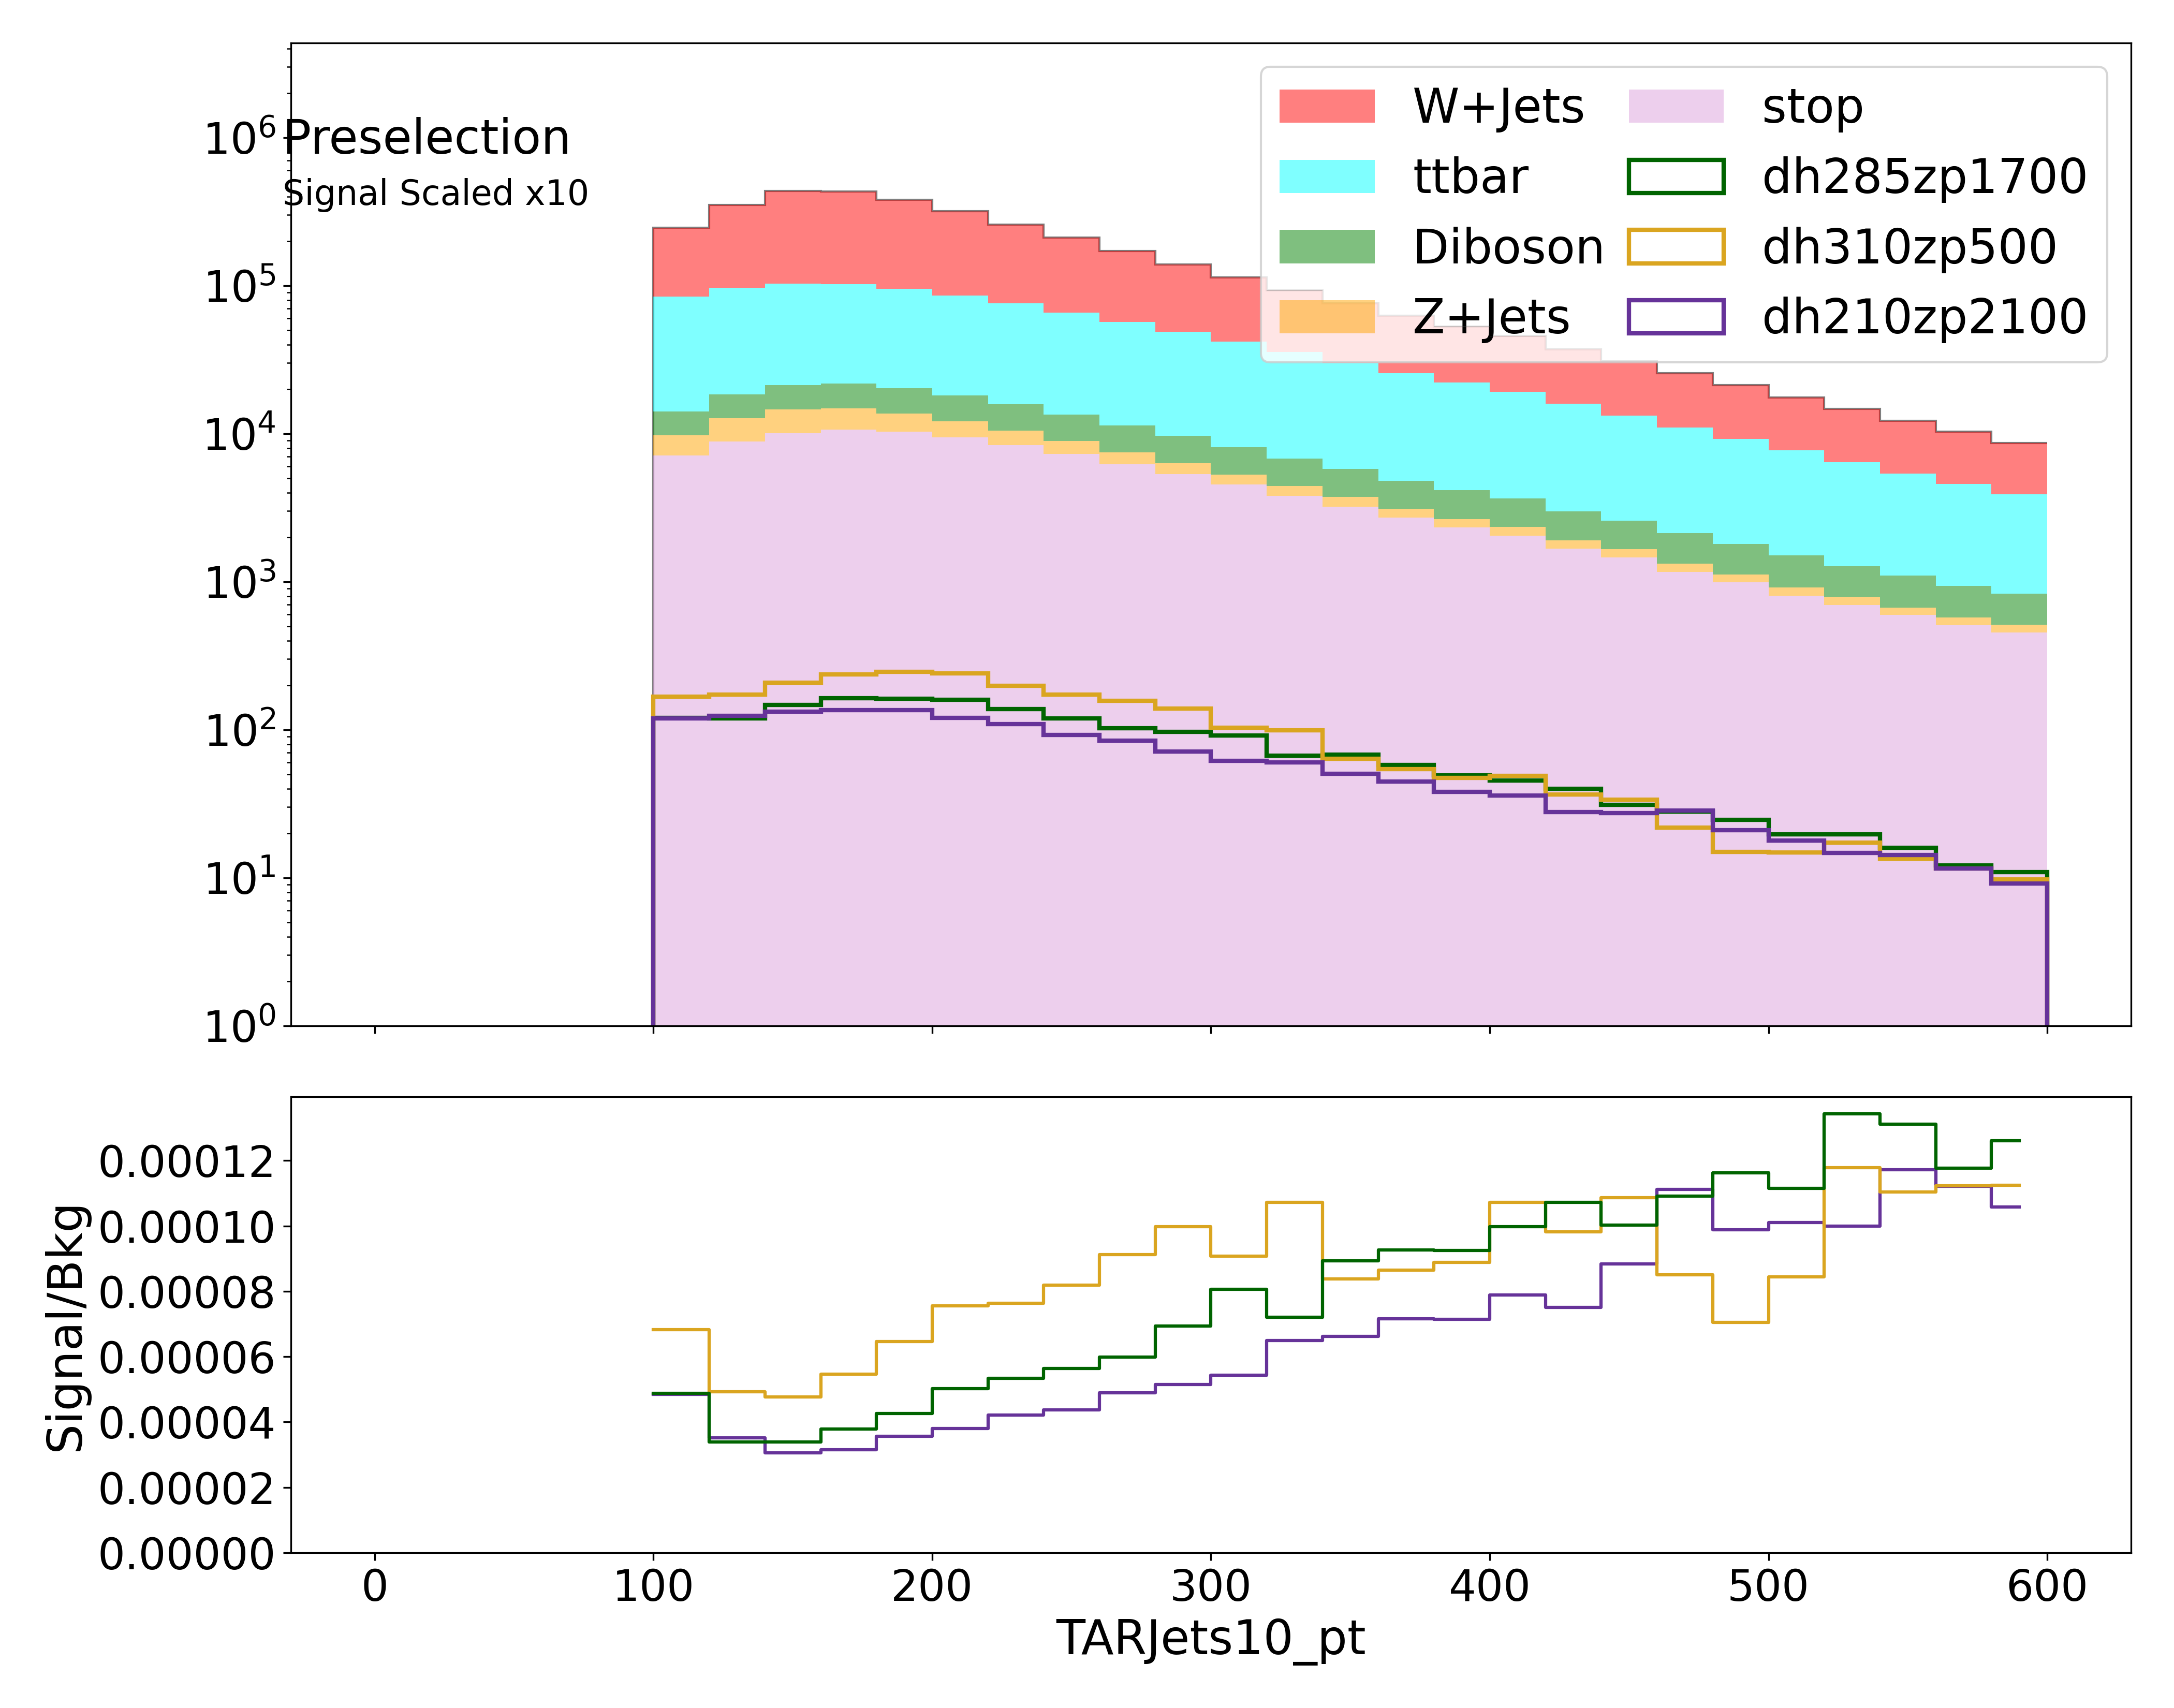
\includegraphics[width = 0.98\textwidth]{Figures/appendix/Preselection/TARJets10_pt.png}
      \caption{$\pT(\text{TAR})$}
      \end{subfigure}
      \begin{subfigure}{0.49\textwidth}
      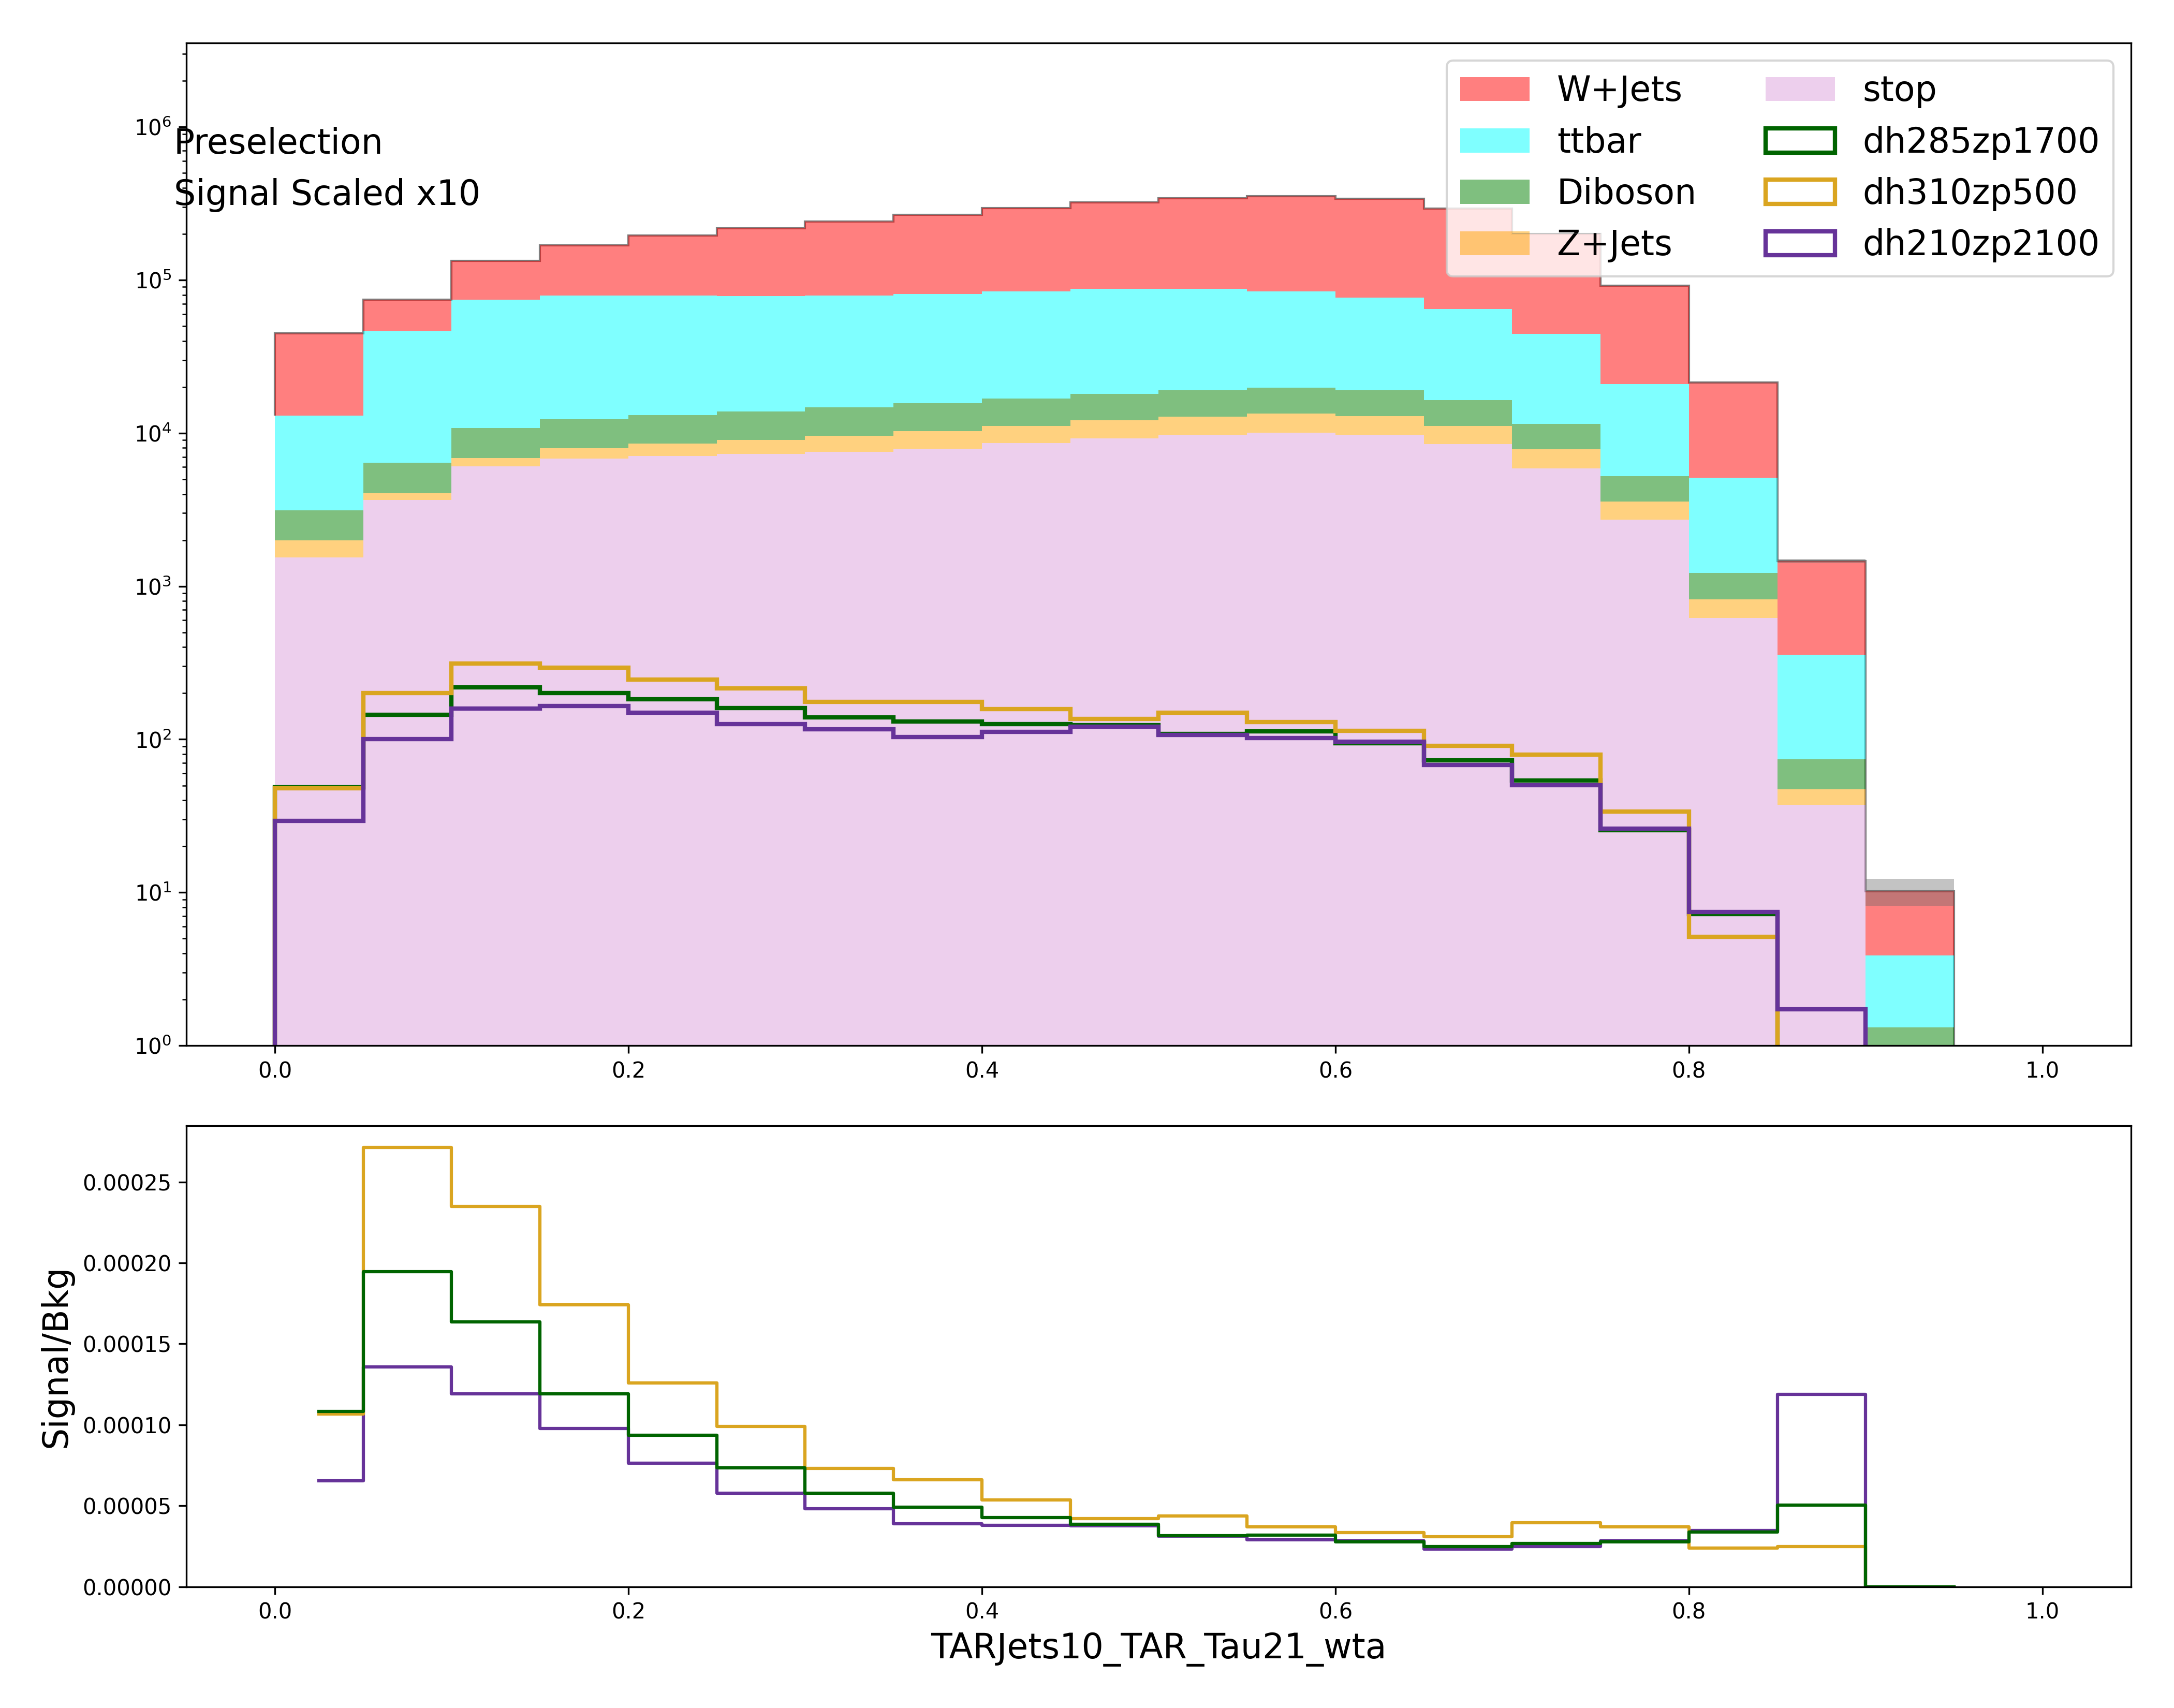
\includegraphics[width = 0.98\textwidth]{Figures/appendix/Preselection/TARJets10_TAR_Tau21_wta.png}
      \caption{$\tau_{21}(\text{TAR})$}
      \end{subfigure}
      \begin{subfigure}{0.49\textwidth}
      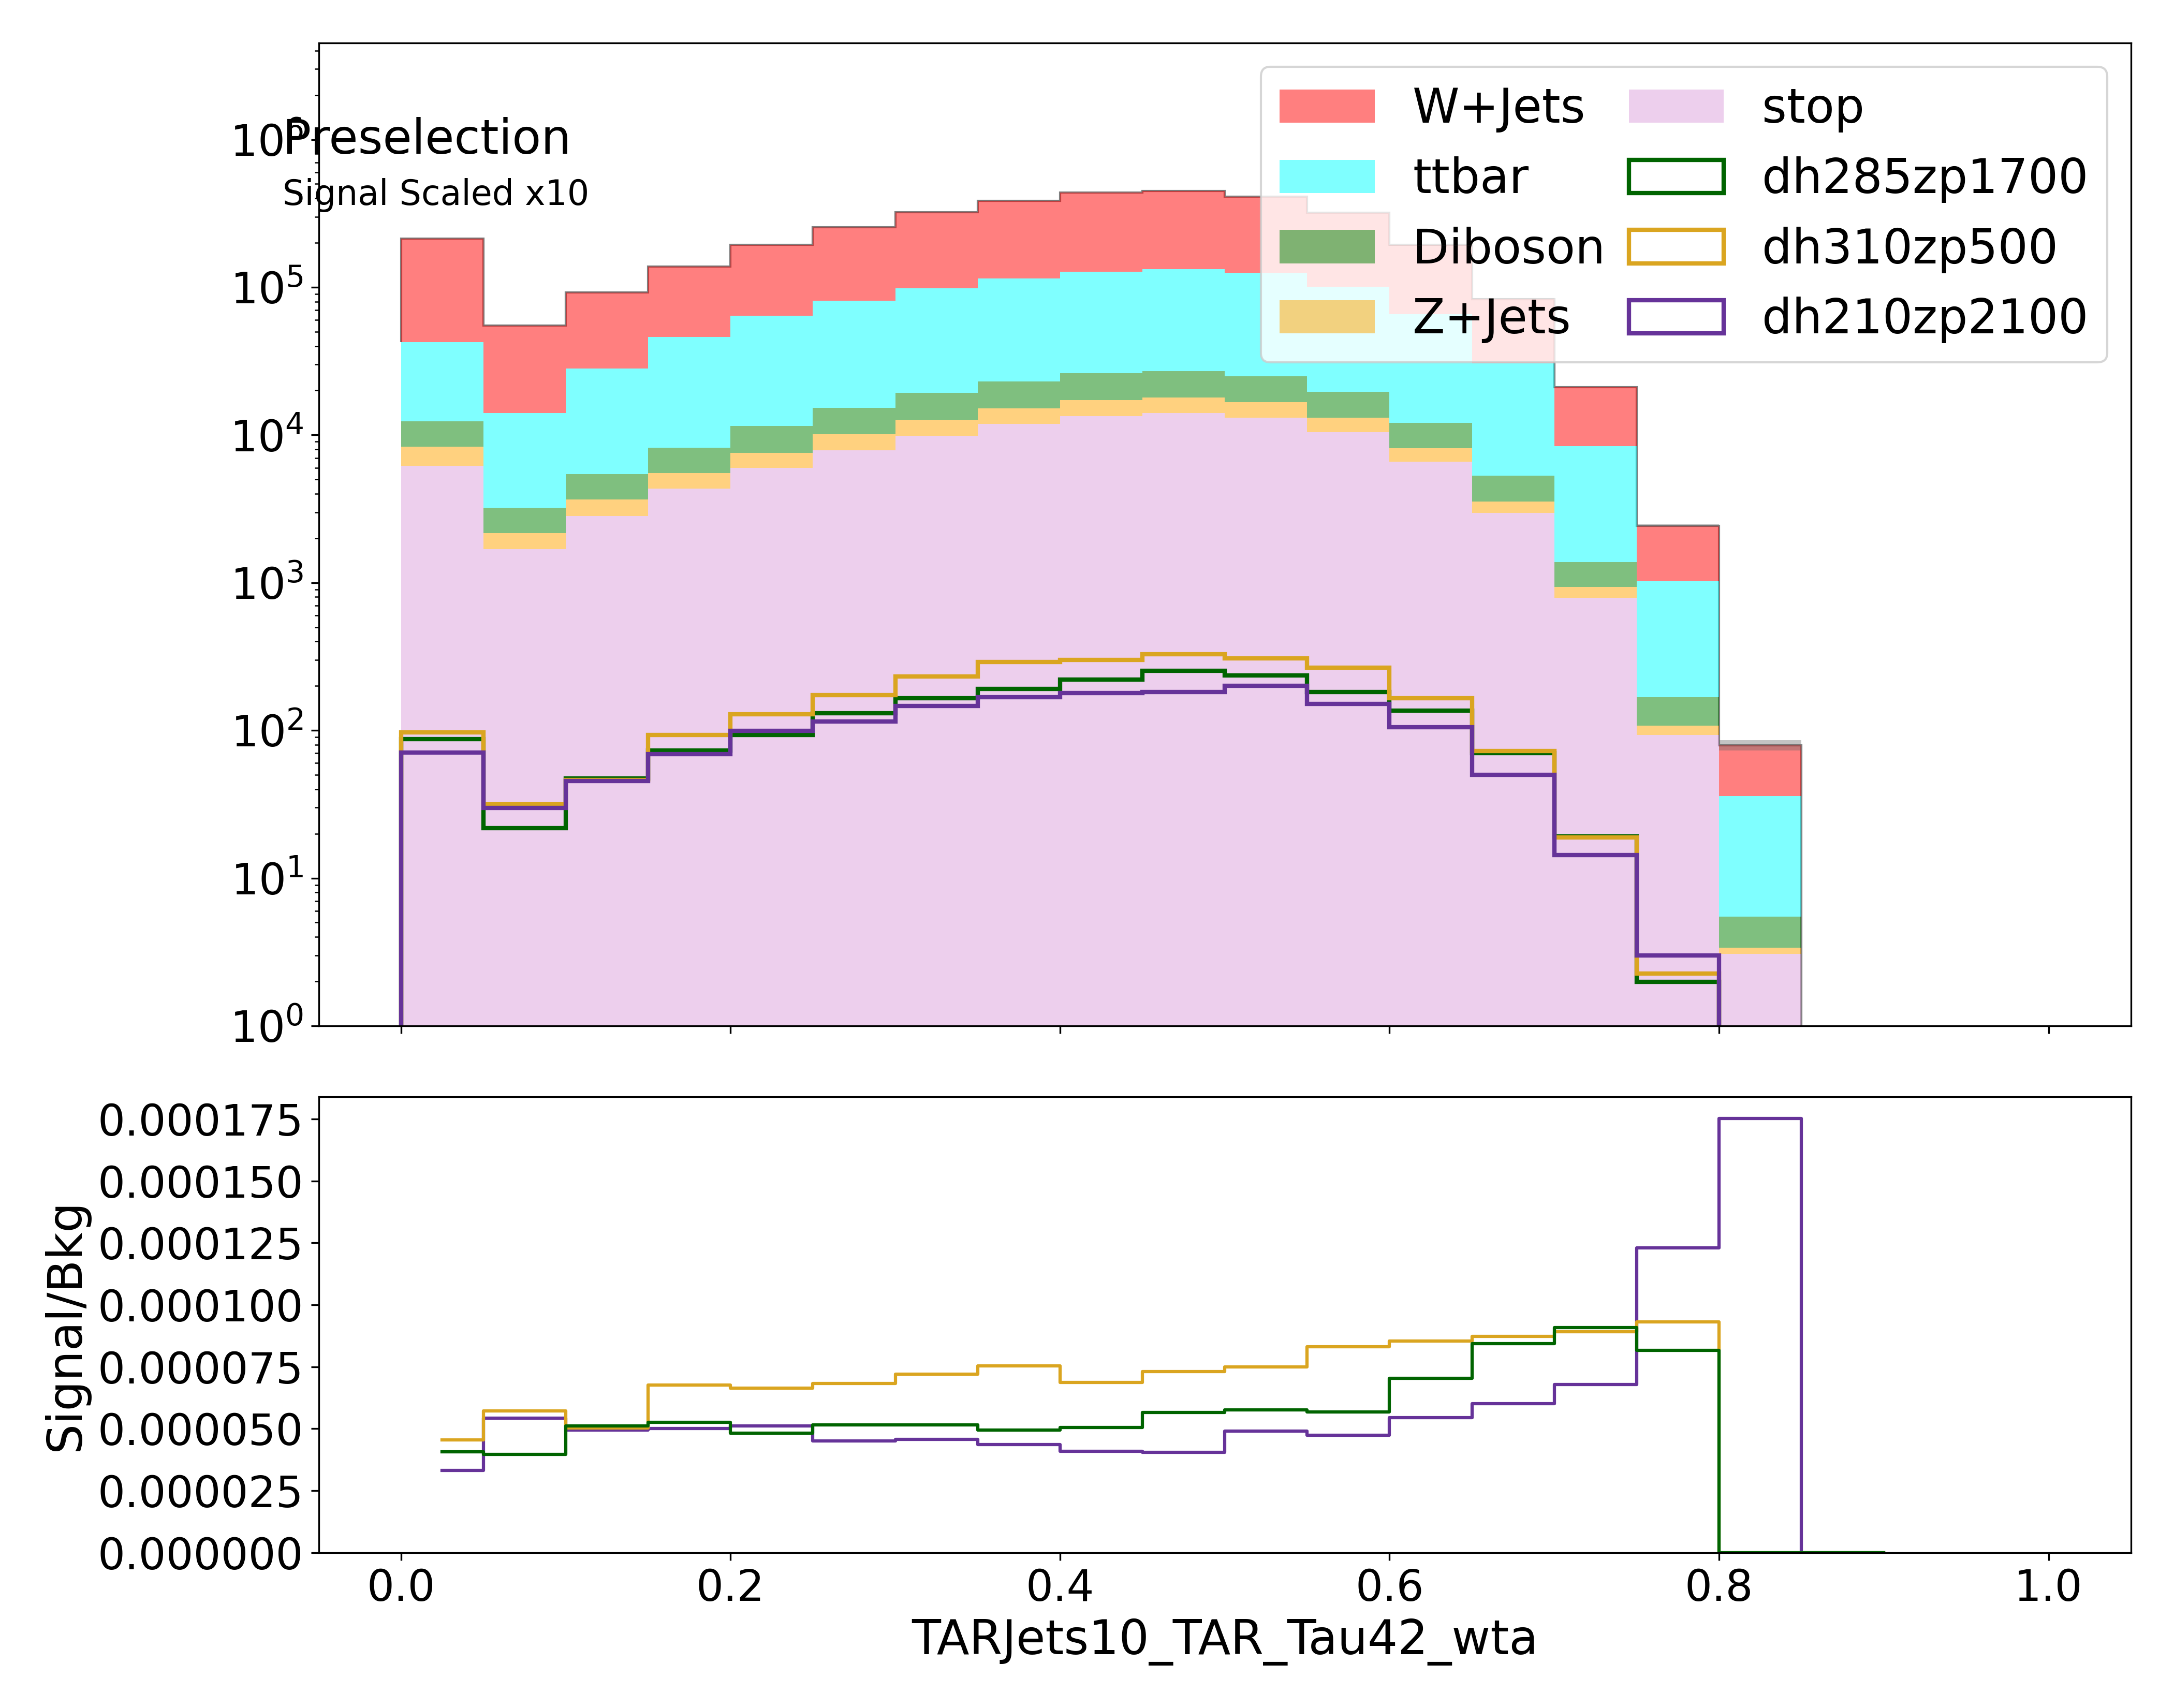
\includegraphics[width = 0.98\textwidth]{Figures/appendix/Preselection/TARJets10_TAR_Tau42_wta.png}
      \caption{$\tau_{42}(\text{TAR})$}
      \end{subfigure}

      \caption{Preselection level distribuitions.}
      \label{fig:Presel2}
    \end{figure}

    \begin{figure}[htbp]
      \centering

         \begin{subfigure}{0.49\textwidth}
         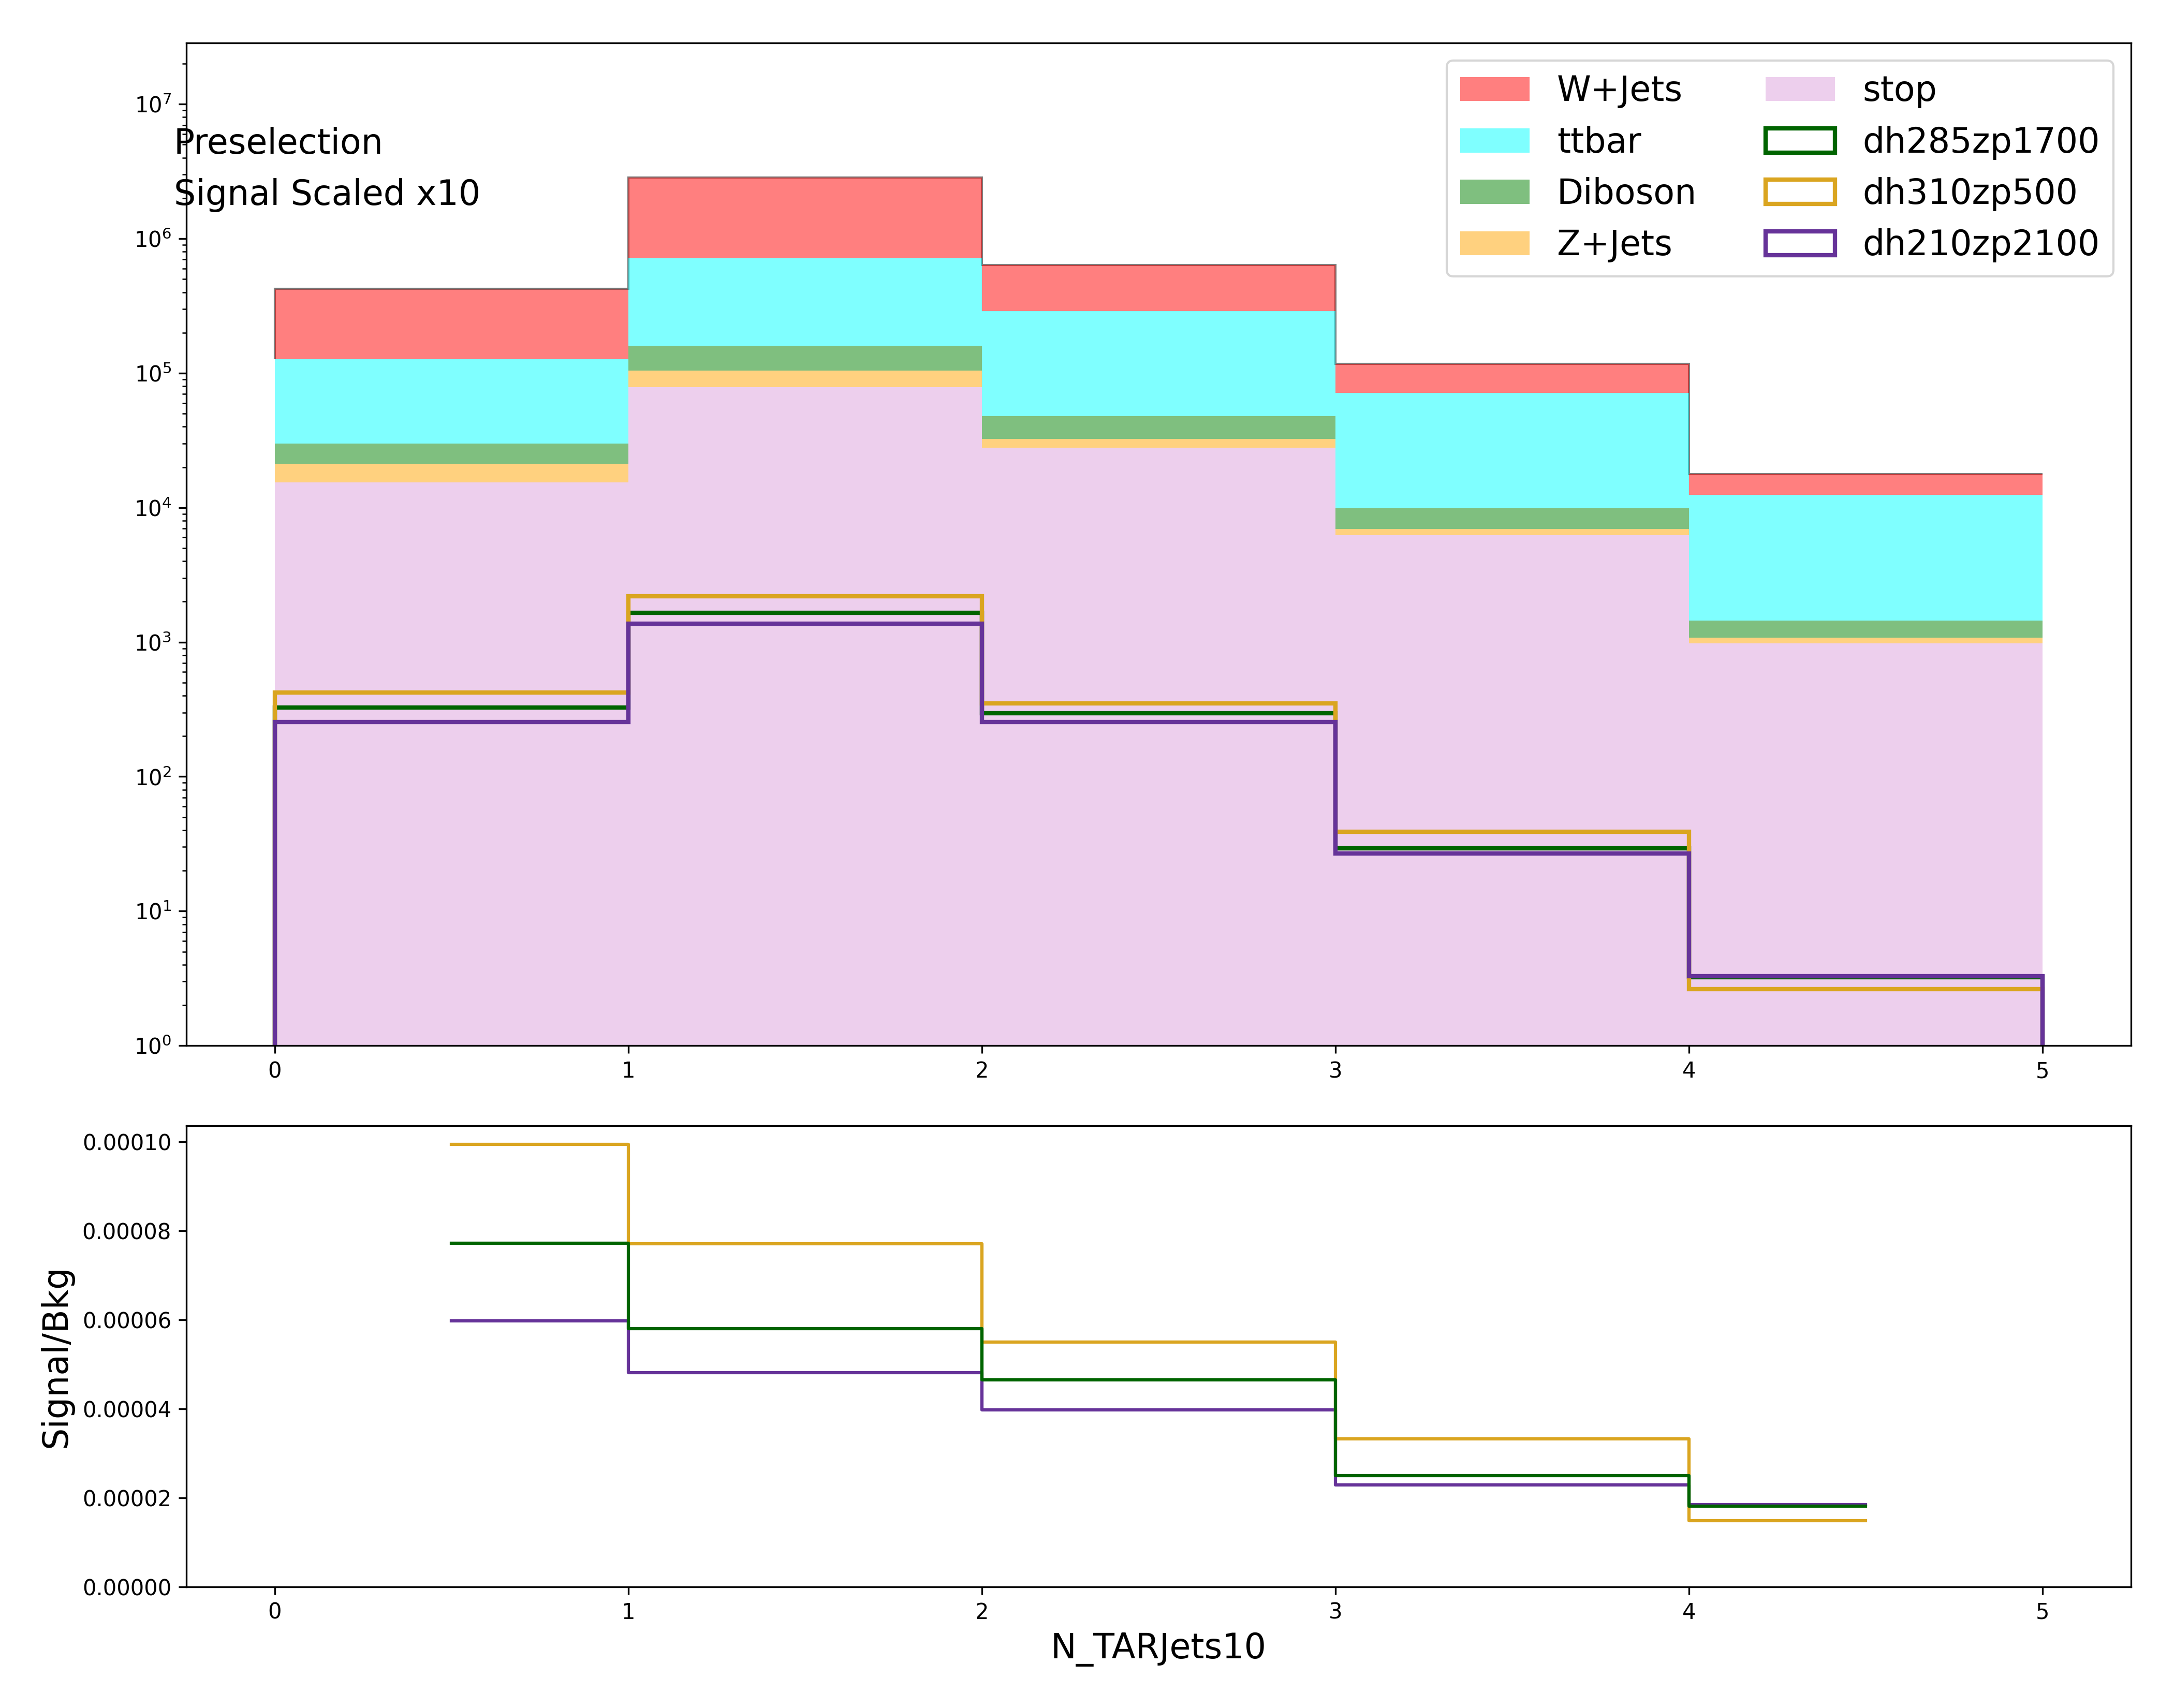
\includegraphics[width = 0.98\textwidth]{Figures/appendix/Preselection/N_TARJets10.png}
         \caption{\NTAR}
         \end{subfigure}
         \begin{subfigure}{0.49\textwidth}
         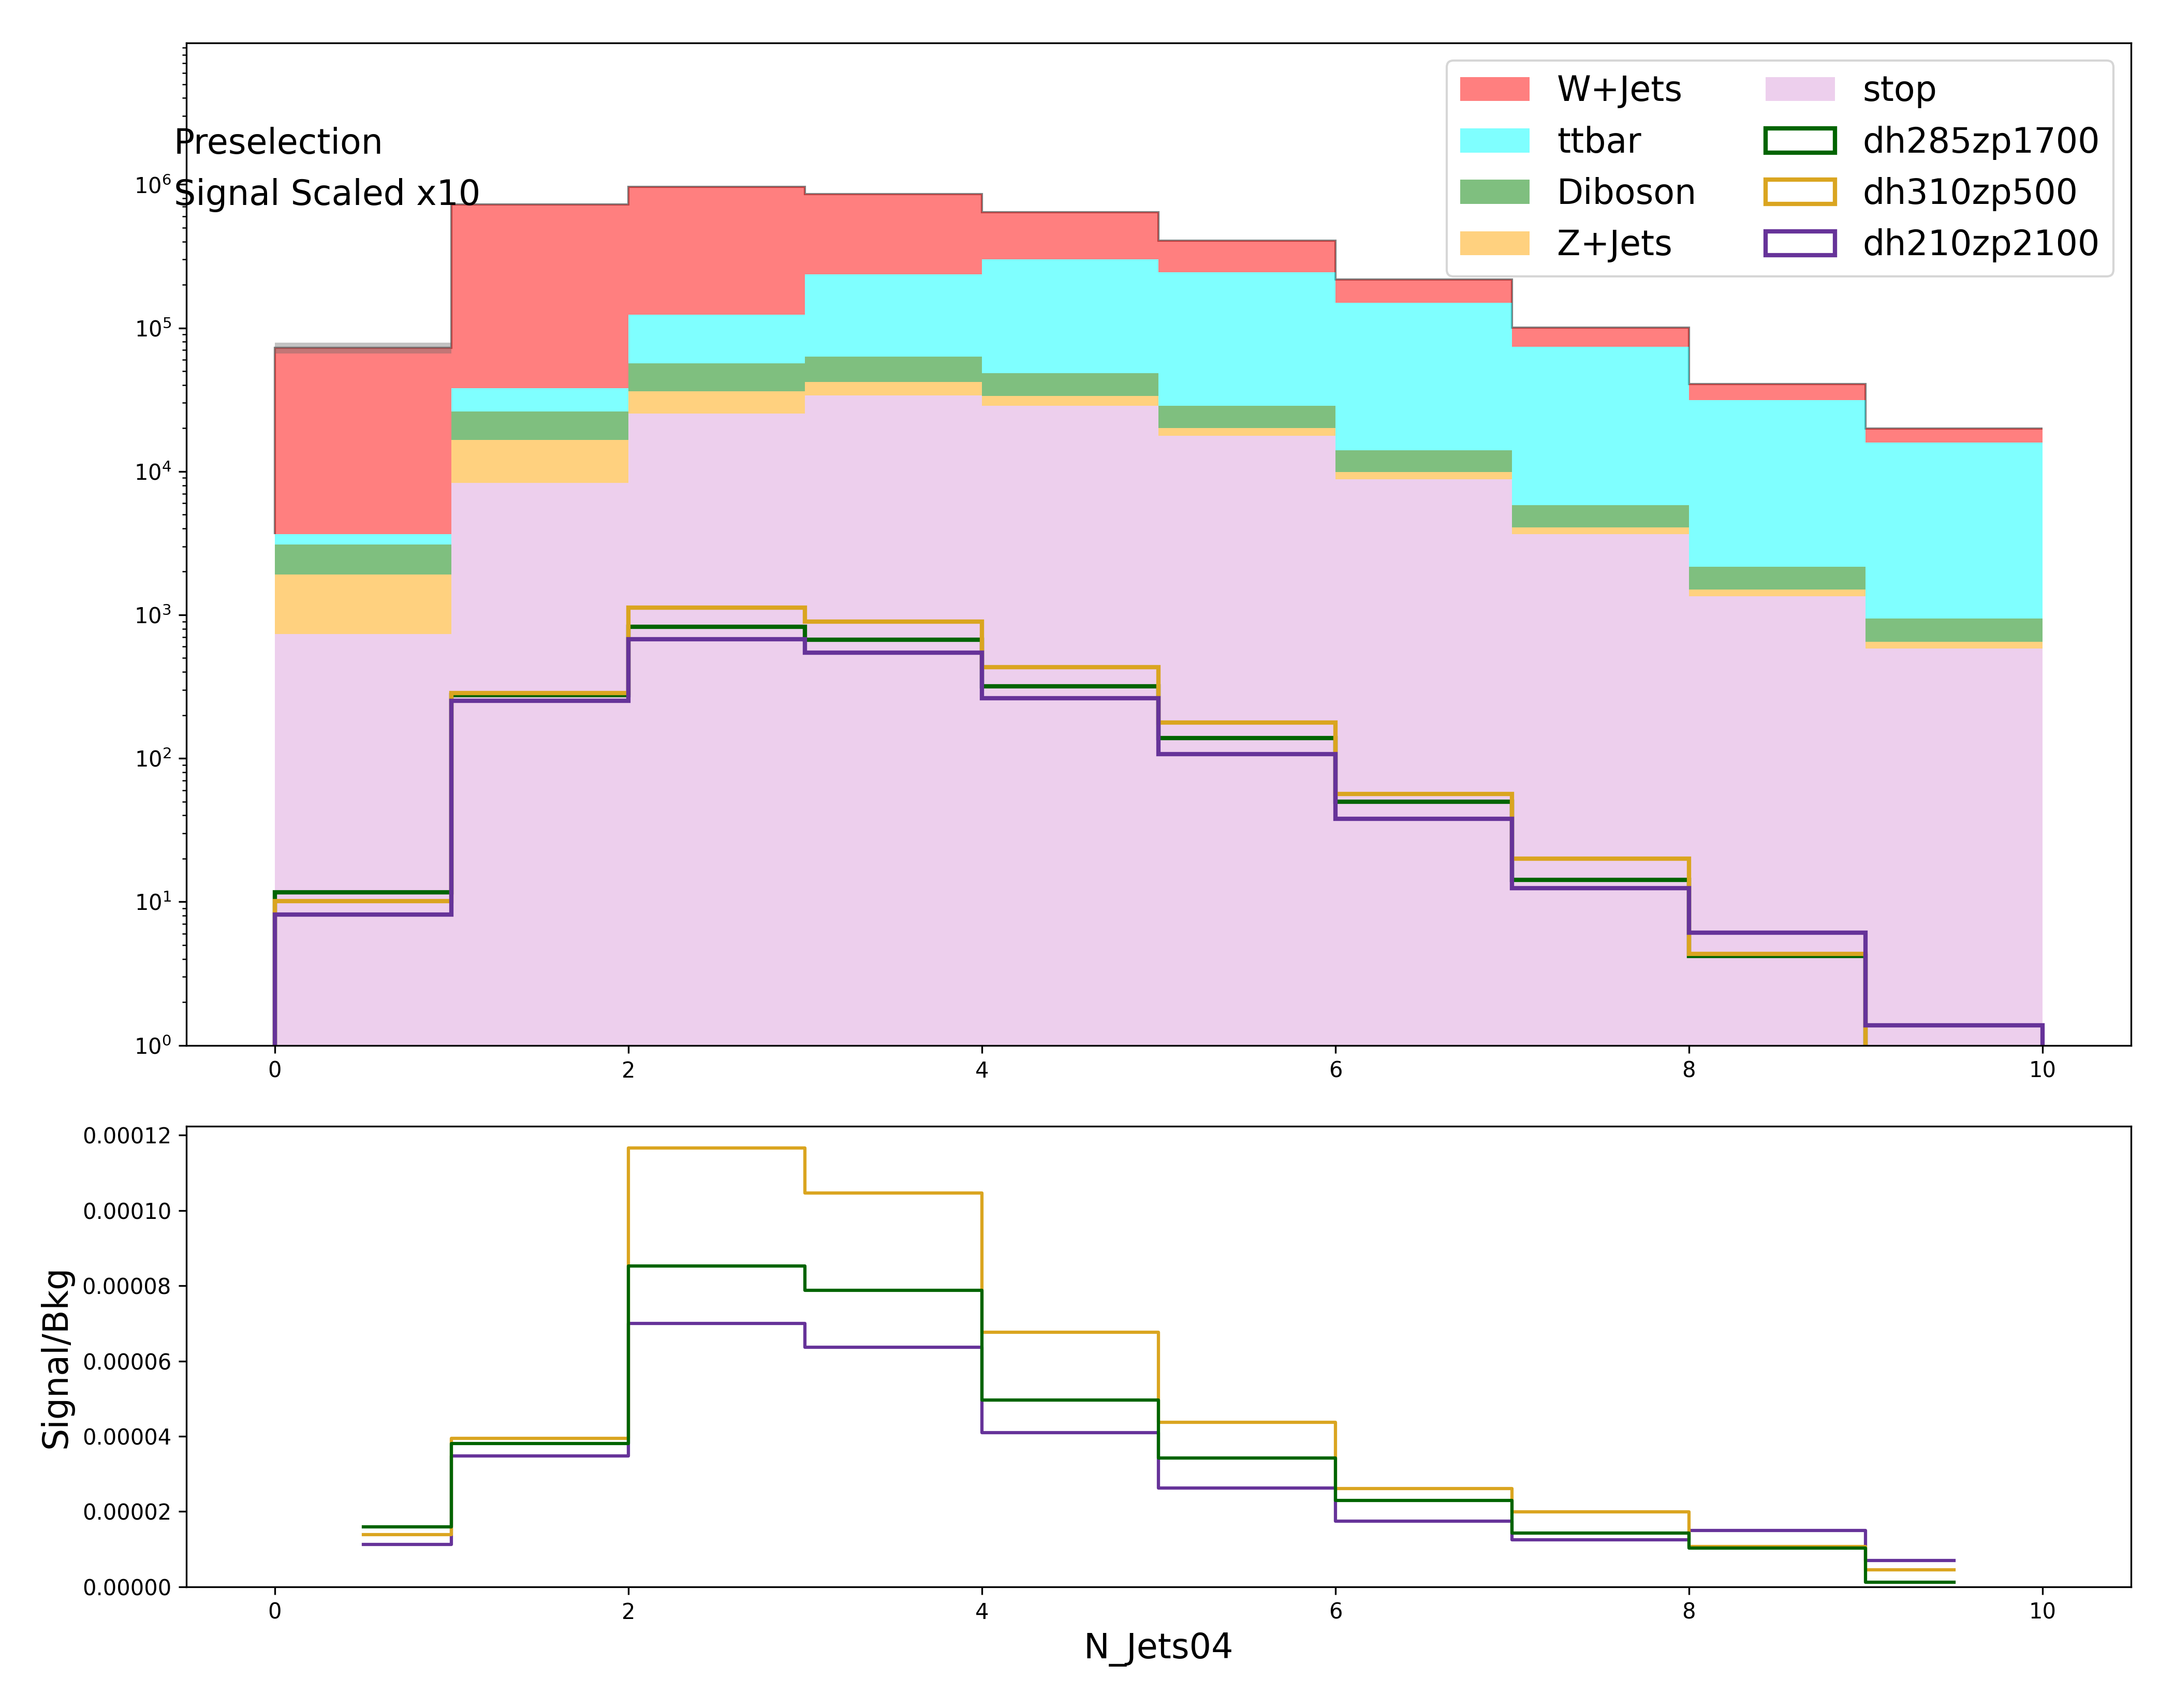
\includegraphics[width = 0.98\textwidth]{Figures/appendix/Preselection/N_Jets04.png}
         \caption{\Njets}
         \end{subfigure}
         \begin{subfigure}{0.49\textwidth}
         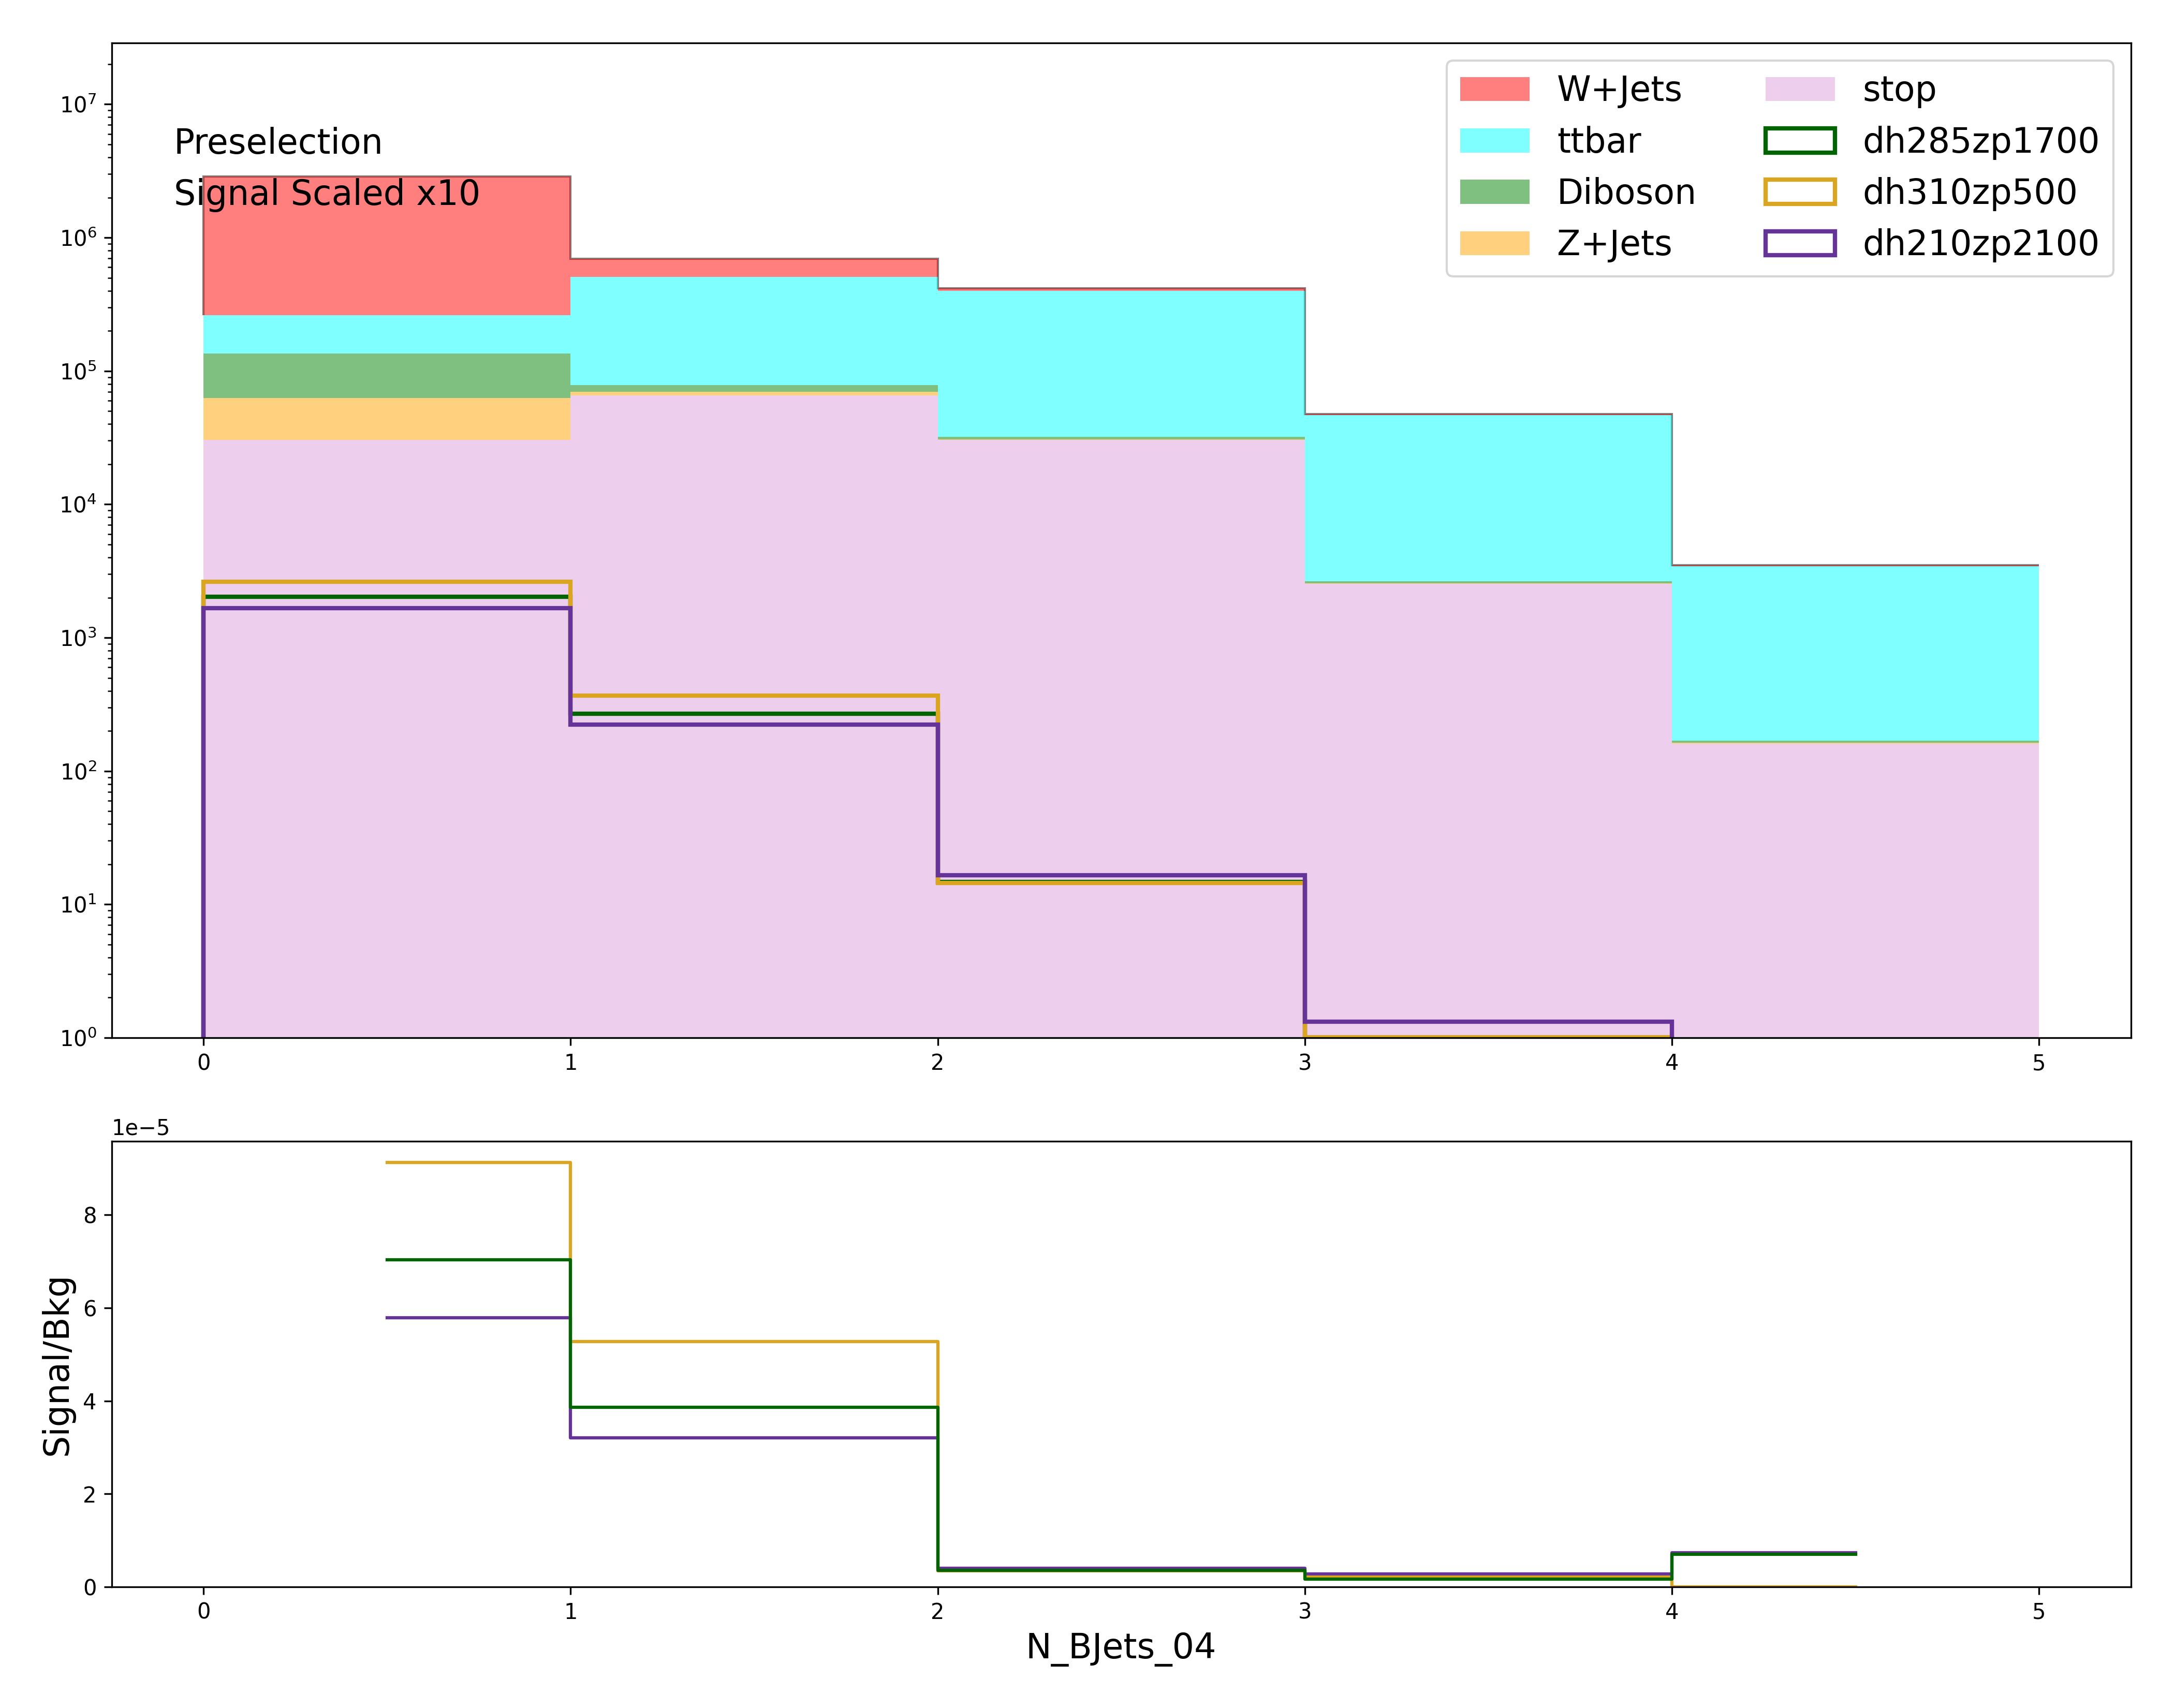
\includegraphics[width = 0.98\textwidth]{Figures/appendix/Preselection/N_BJets_04.png}
         \caption{\ensuremath{N (\text{b-Jets})}\xspace}
         \end{subfigure}
         \begin{subfigure}{0.49\textwidth}
         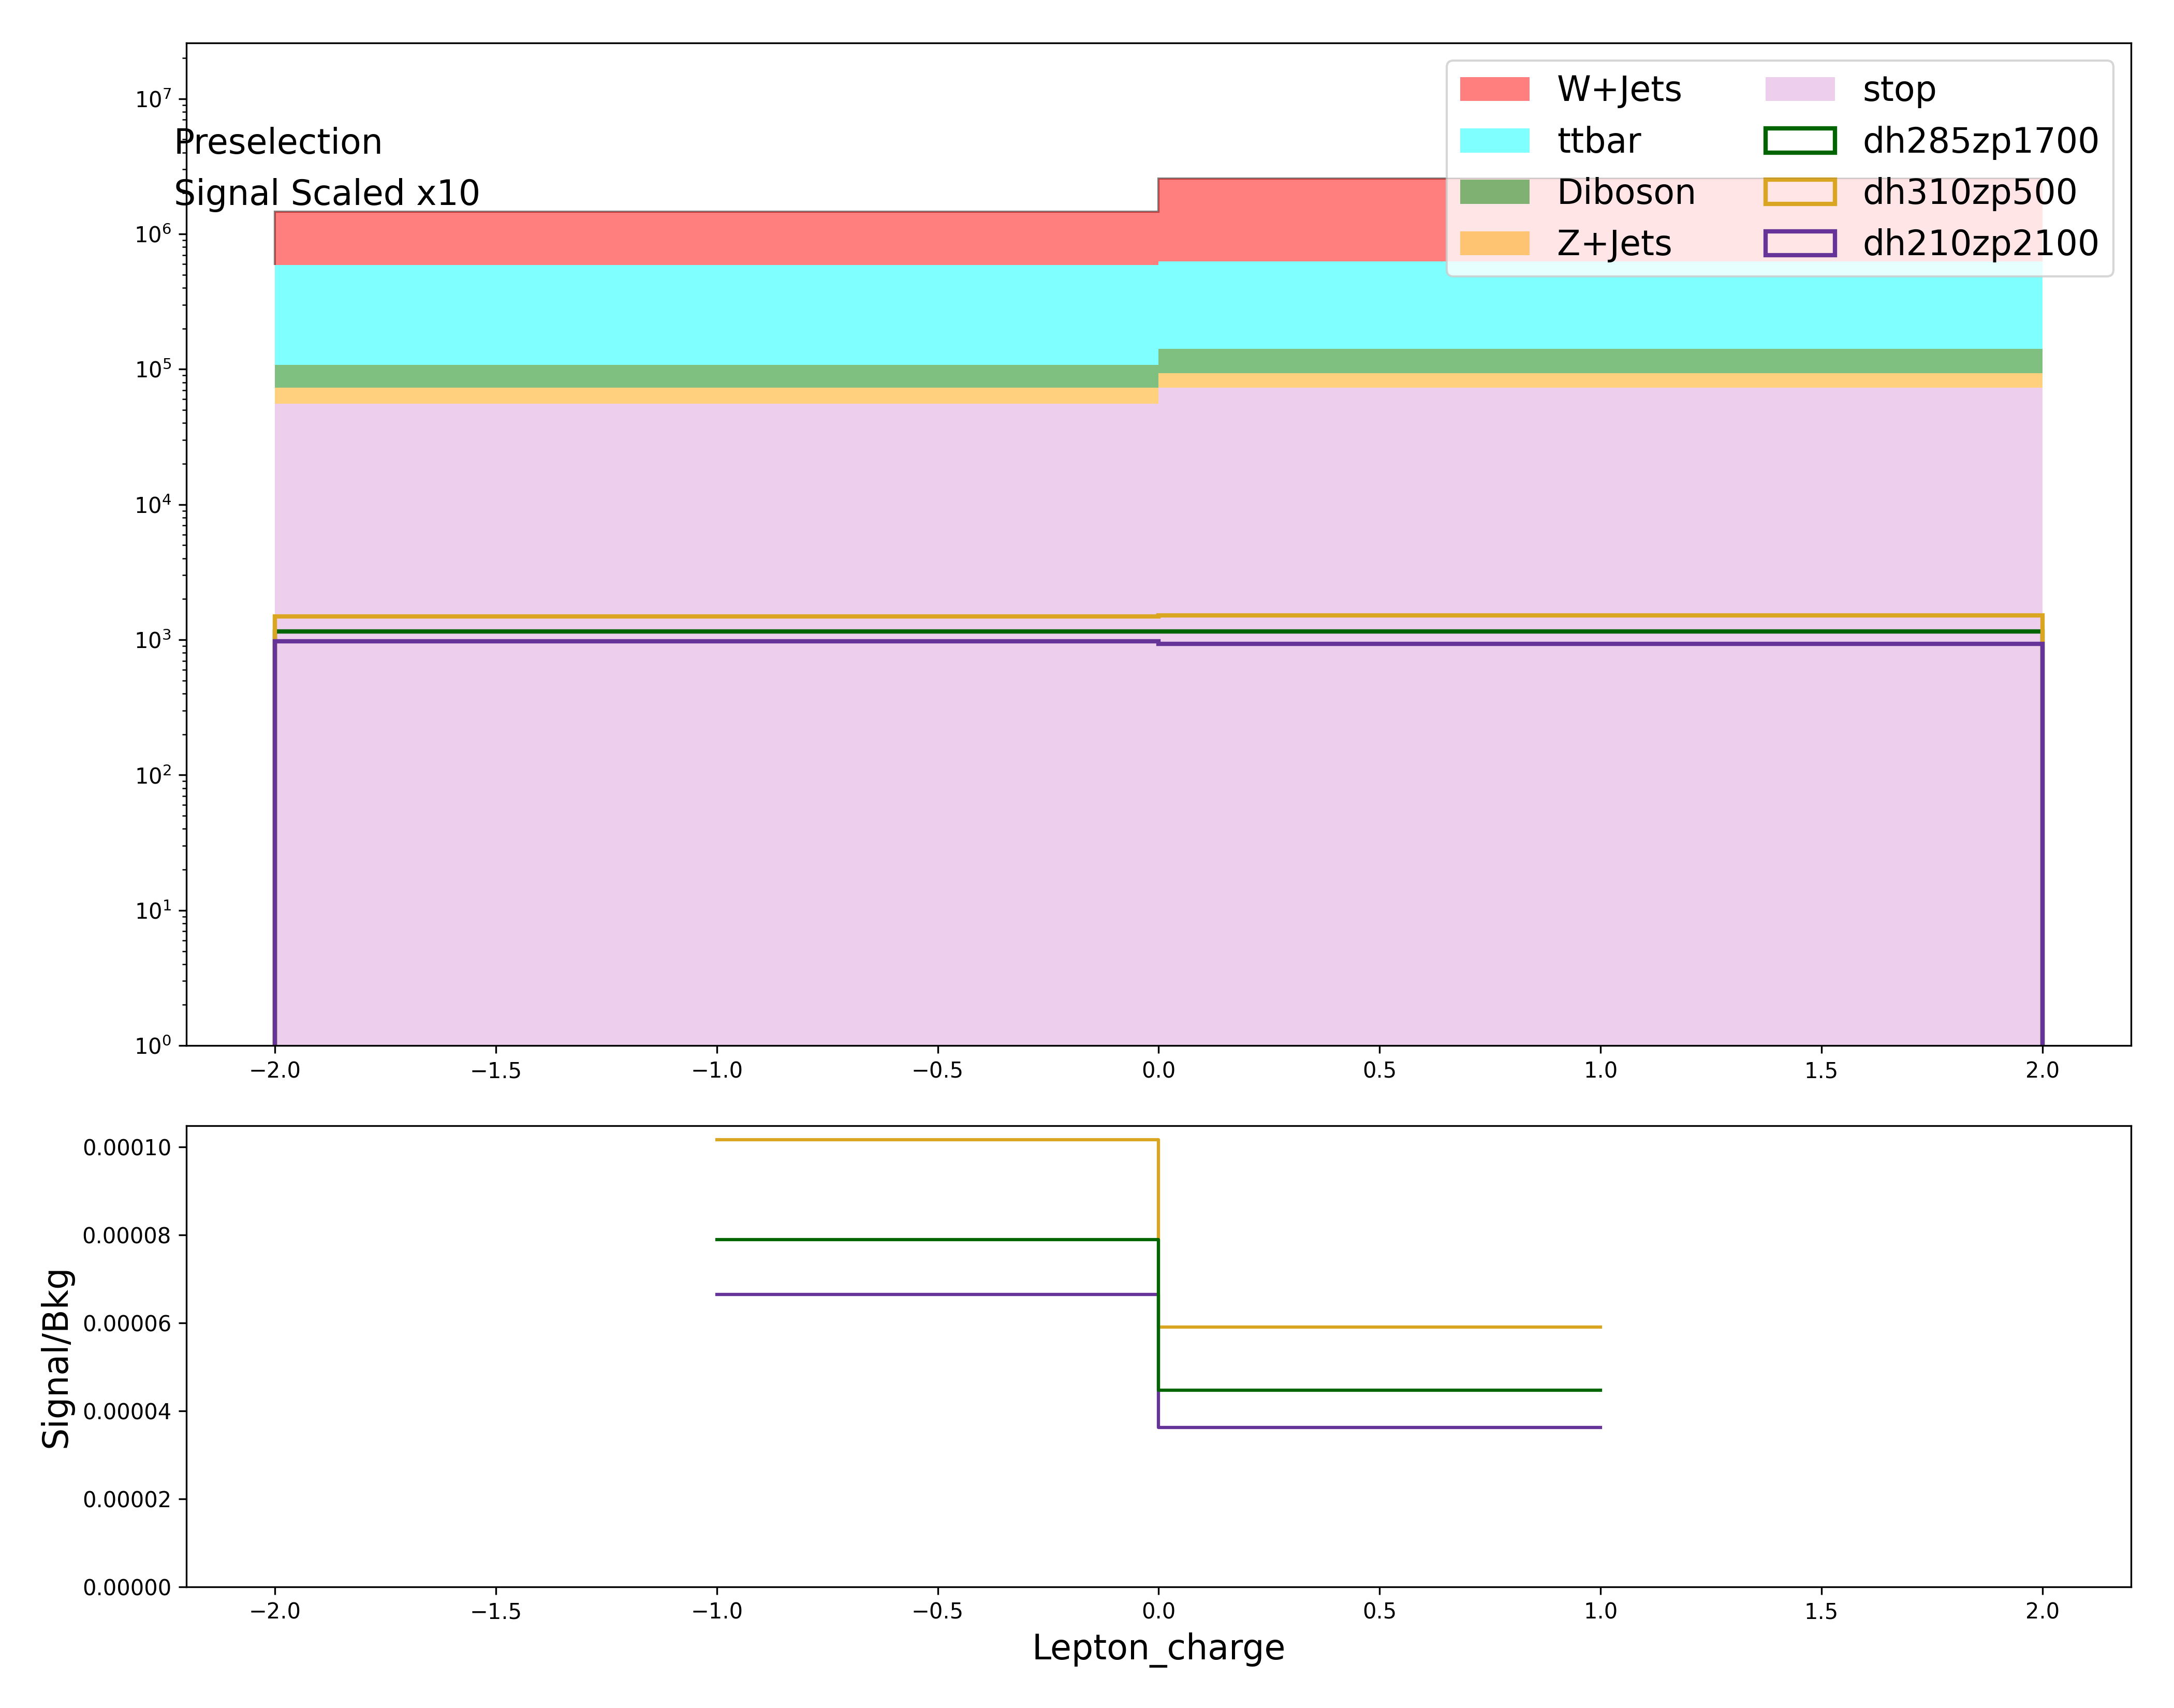
\includegraphics[width = 0.98\textwidth]{Figures/appendix/Preselection/Lepton_charge.png}
         \caption{$\text{charge}(\ell)$}
         \end{subfigure}

         \caption{Preselection level distribuitions.}
         \label{fig:Presel3}
      \end{figure}
\FloatBarrier

\section{Data-MC Comparisons in Control Regions}
\label{section:datamc}
The following section contains plots comparing data and MC distributions in the control regions. MC events are normalized to the luminosity measured in data as described in Chapter \ref{chapter:ana_prep} Subsection \ref{subsection:mc_scaling}. The uncertainties shown on both data and MC events in these plots are purely statistical and do not include uncertainties on the modelling of background events, which impact the cross-section of the different categories of background events. Some statistically significant differences between data and MC are therefore not unexpected.
\subsection{\ttbar Control Regions}

\begin{figure}[htbp]
  \centering

     \begin{subfigure}{0.49\textwidth}
     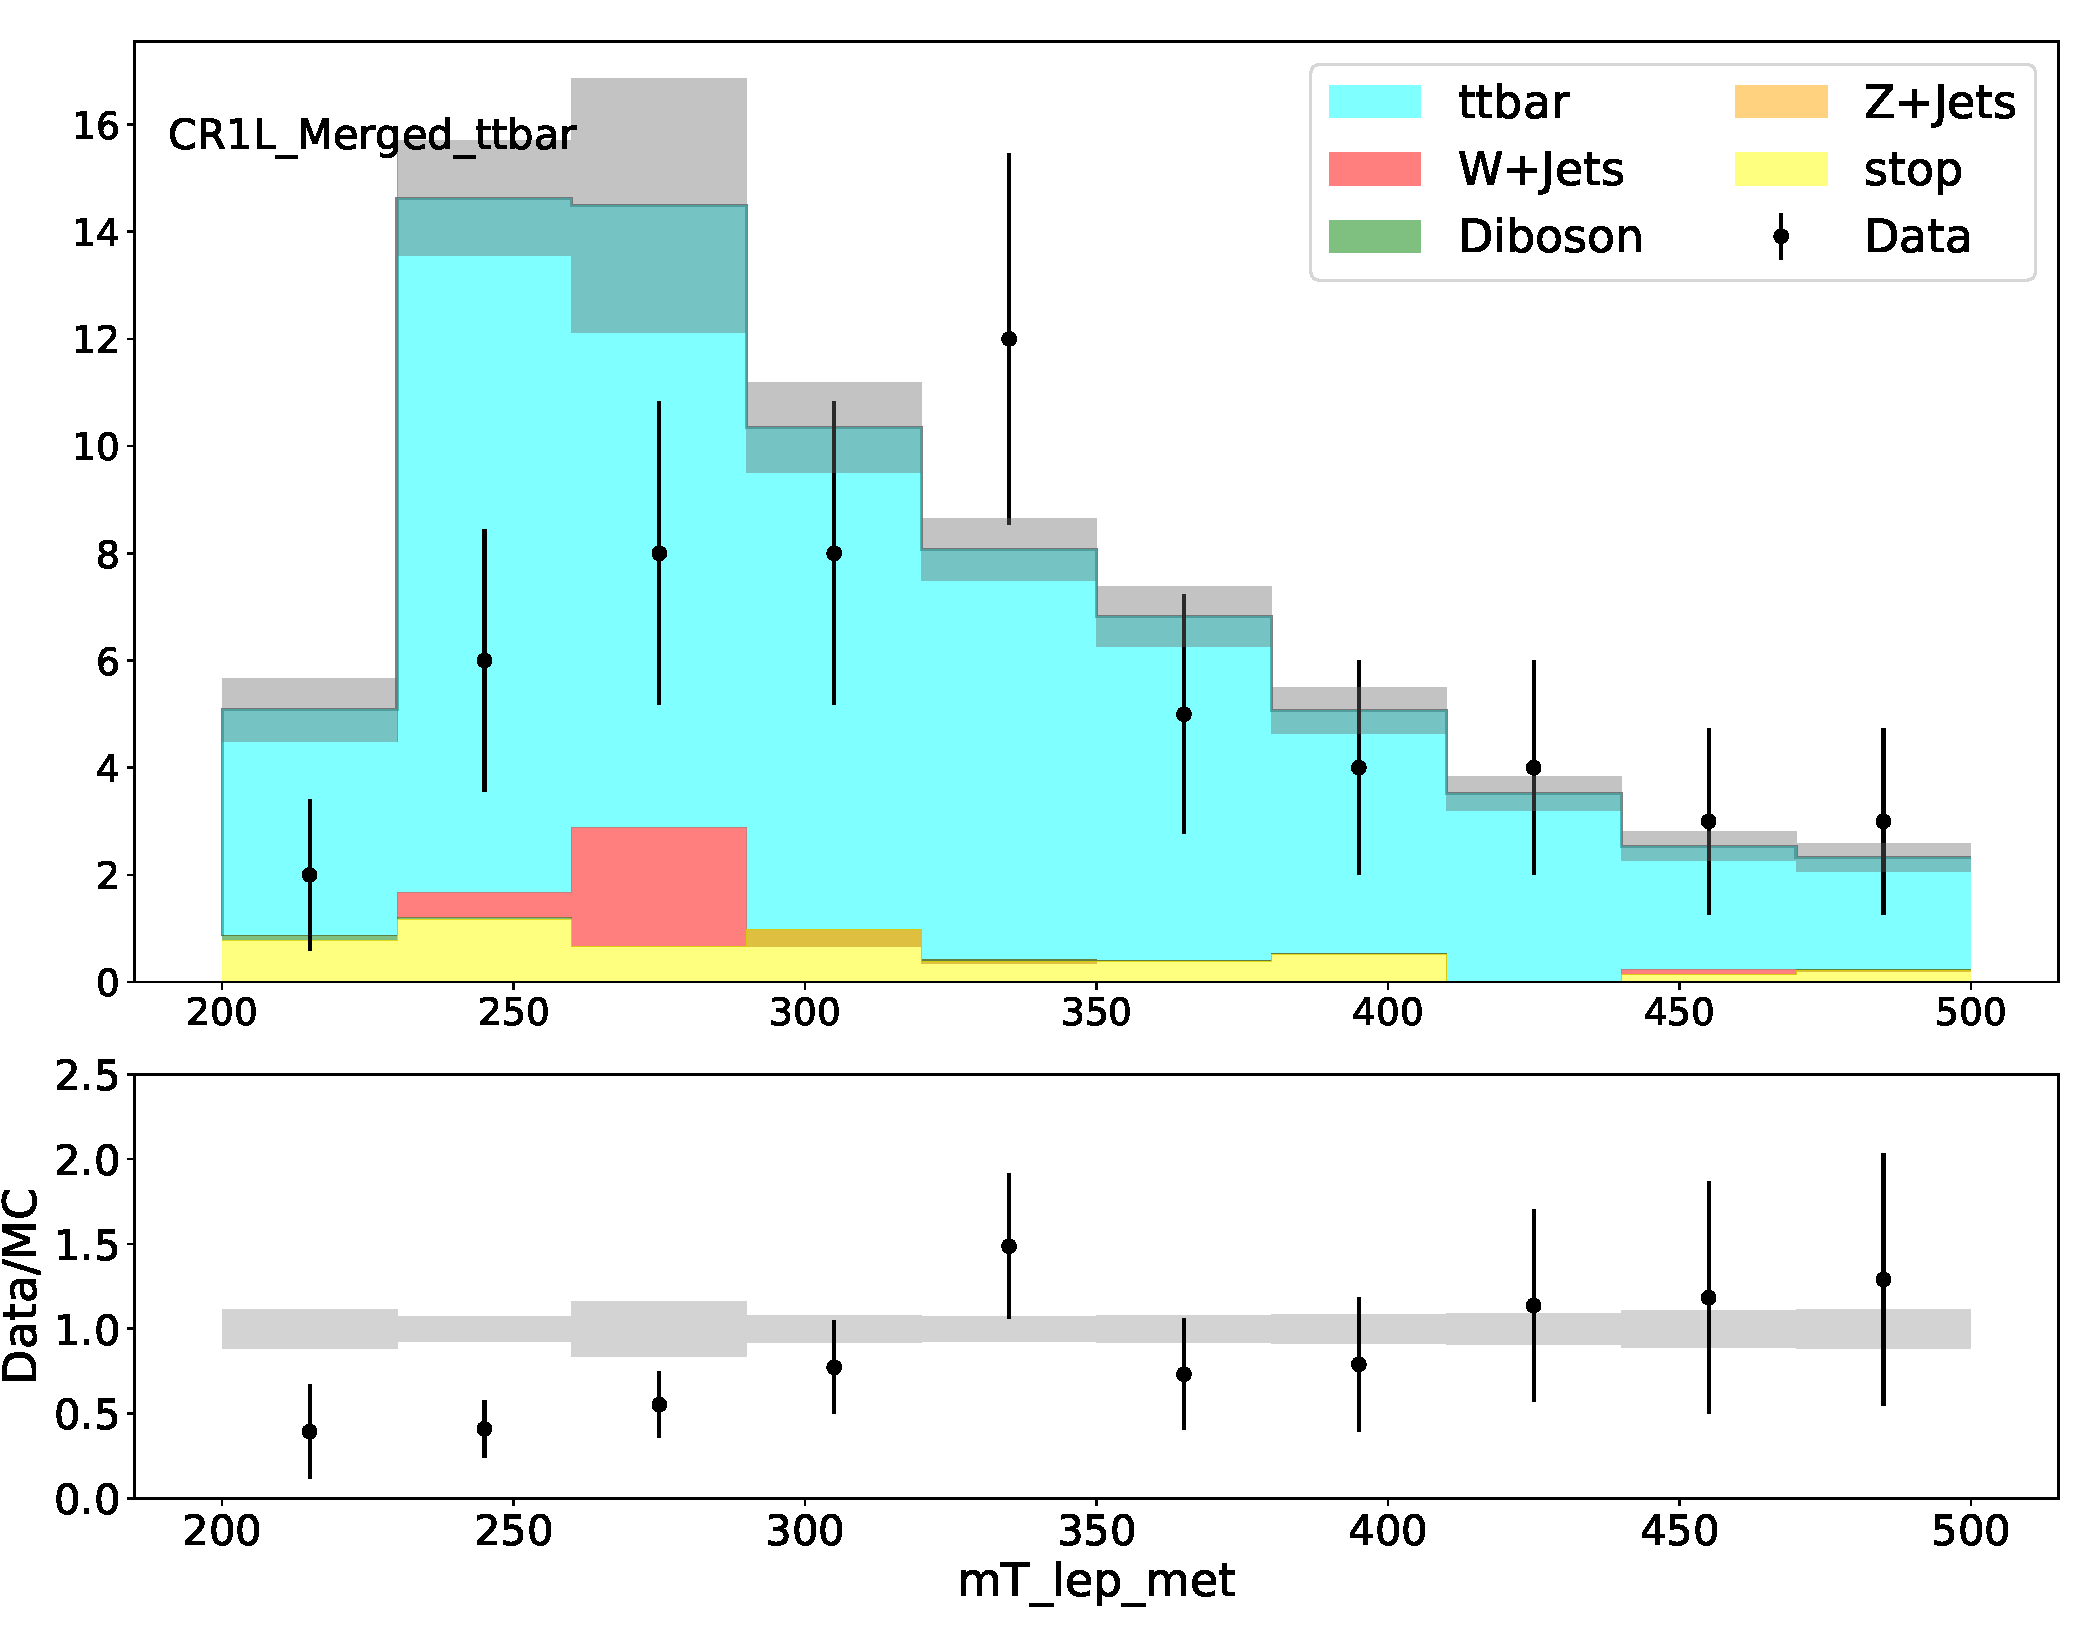
\includegraphics[width = 0.98\textwidth]{Figures/4/datamc/CR1L_Merged_ttbar/mT_lep_met.pdf}
     \caption{\mtlepmet}
     \end{subfigure}
     \begin{subfigure}{0.49\textwidth}
     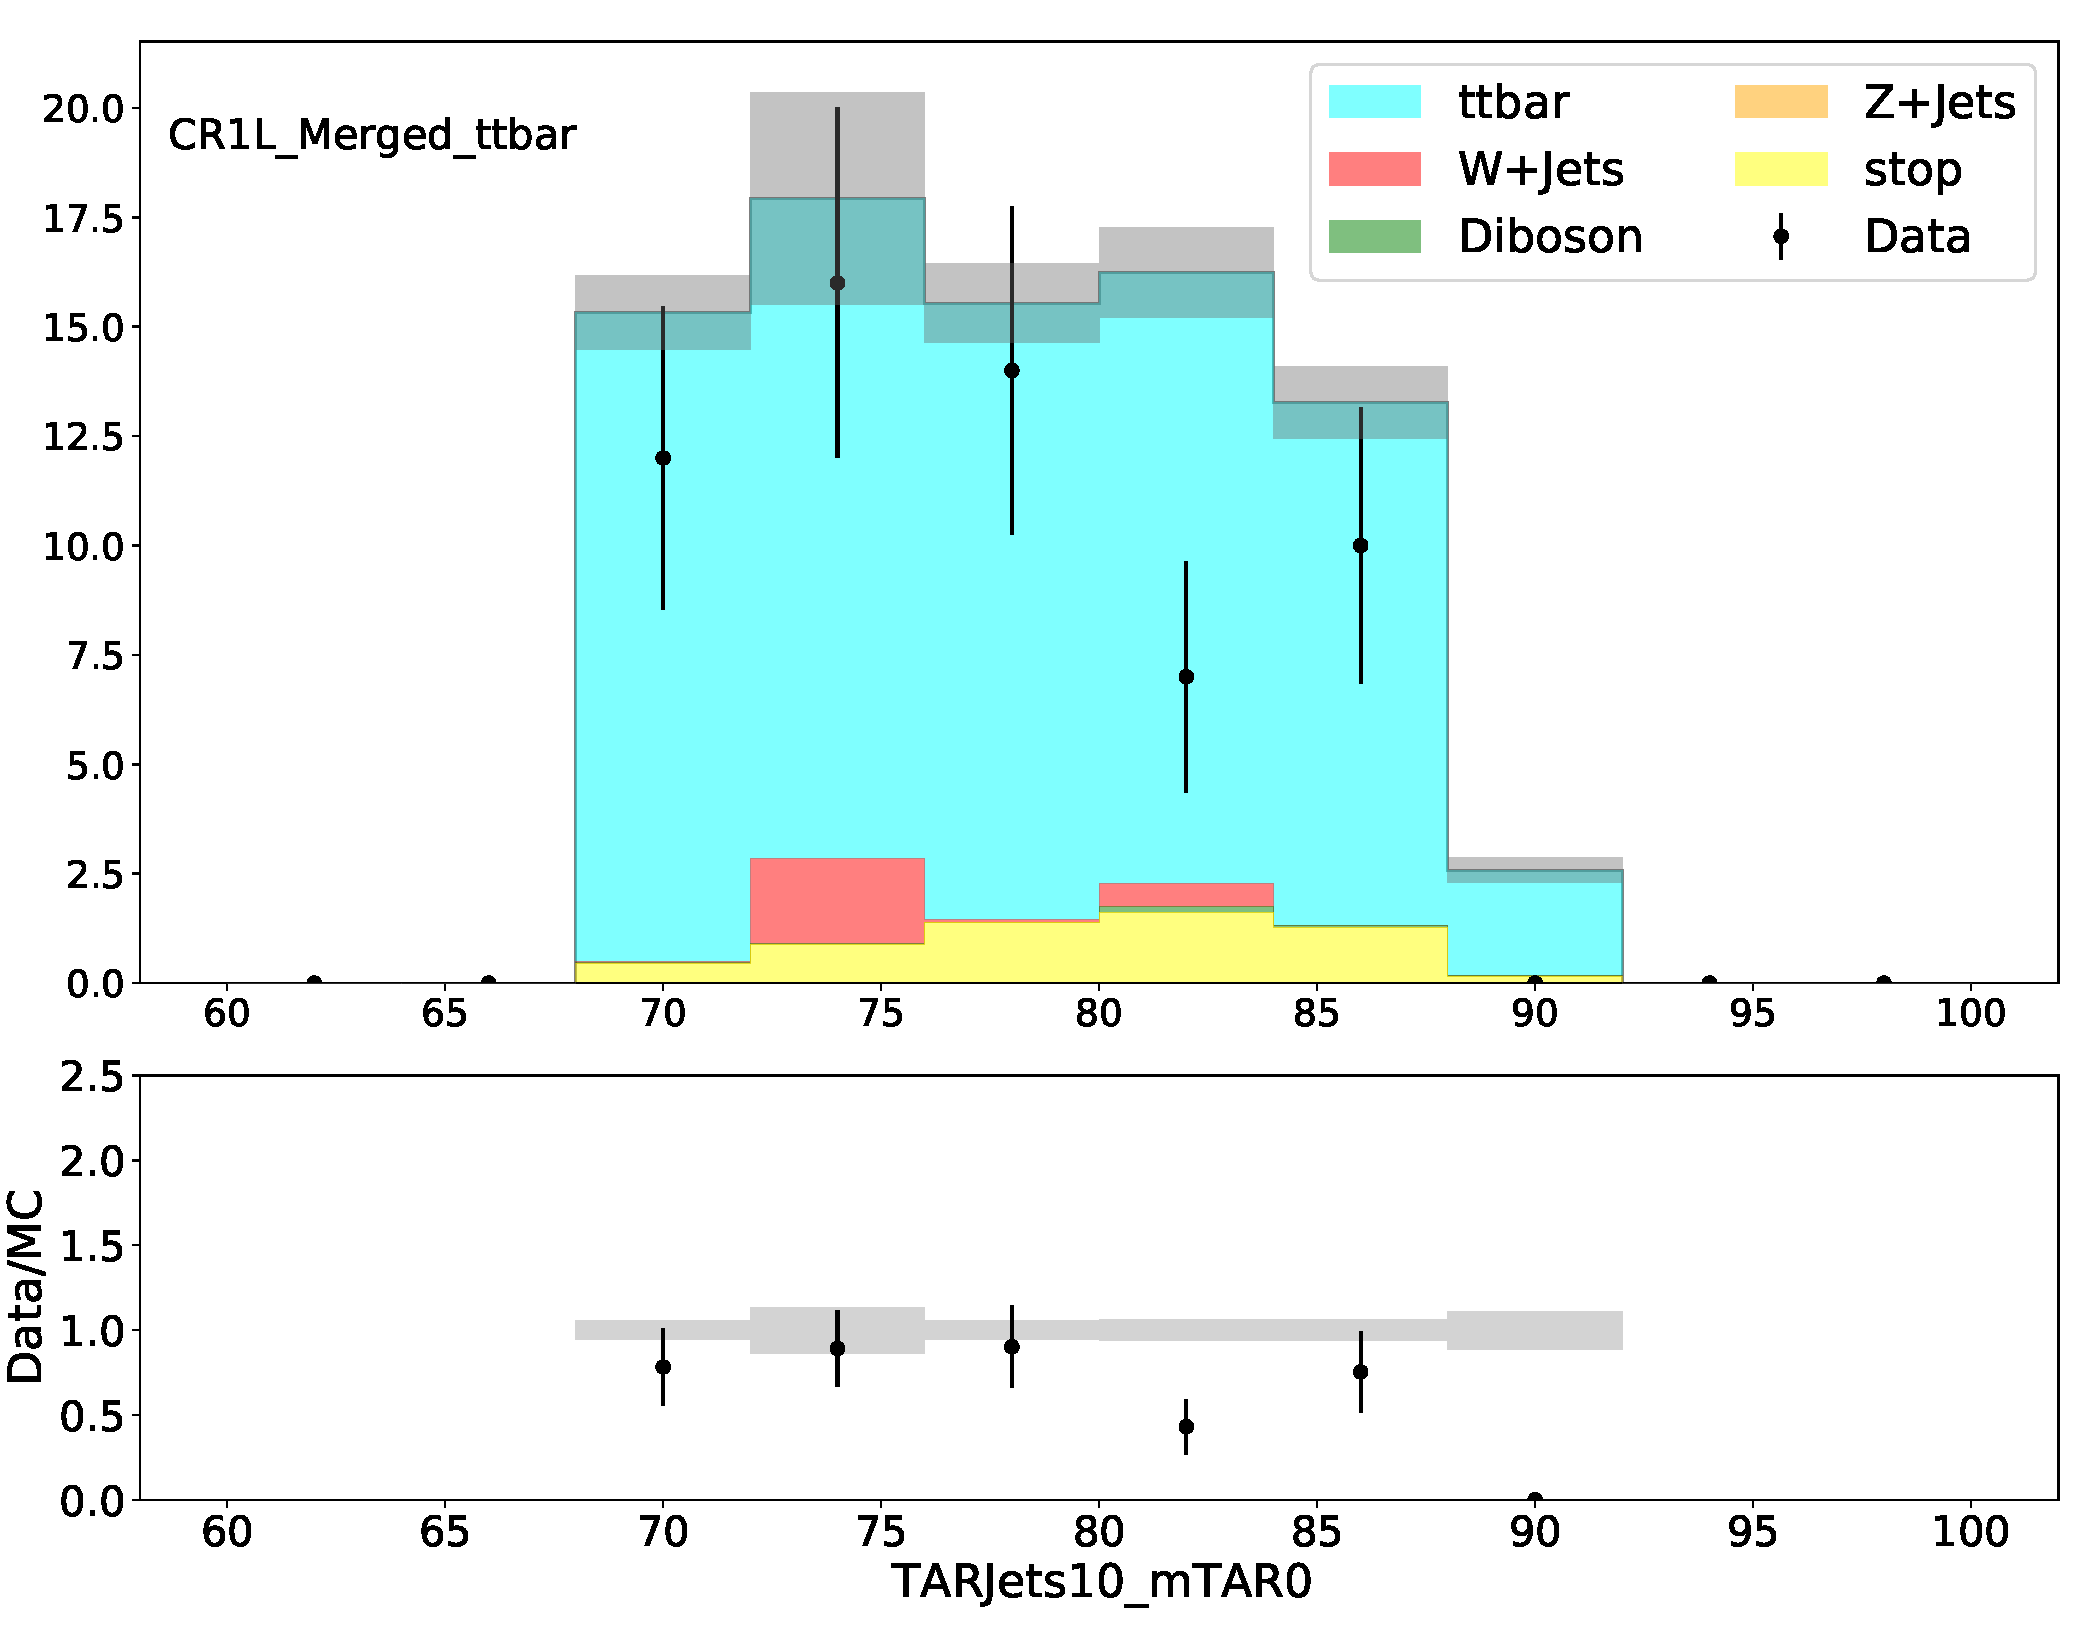
\includegraphics[width = 0.98\textwidth]{Figures/4/datamc/CR1L_Merged_ttbar/TARJets10_mTAR0.pdf}
     \caption{\mTAR}
     \end{subfigure}
     \begin{subfigure}{0.49\textwidth}
     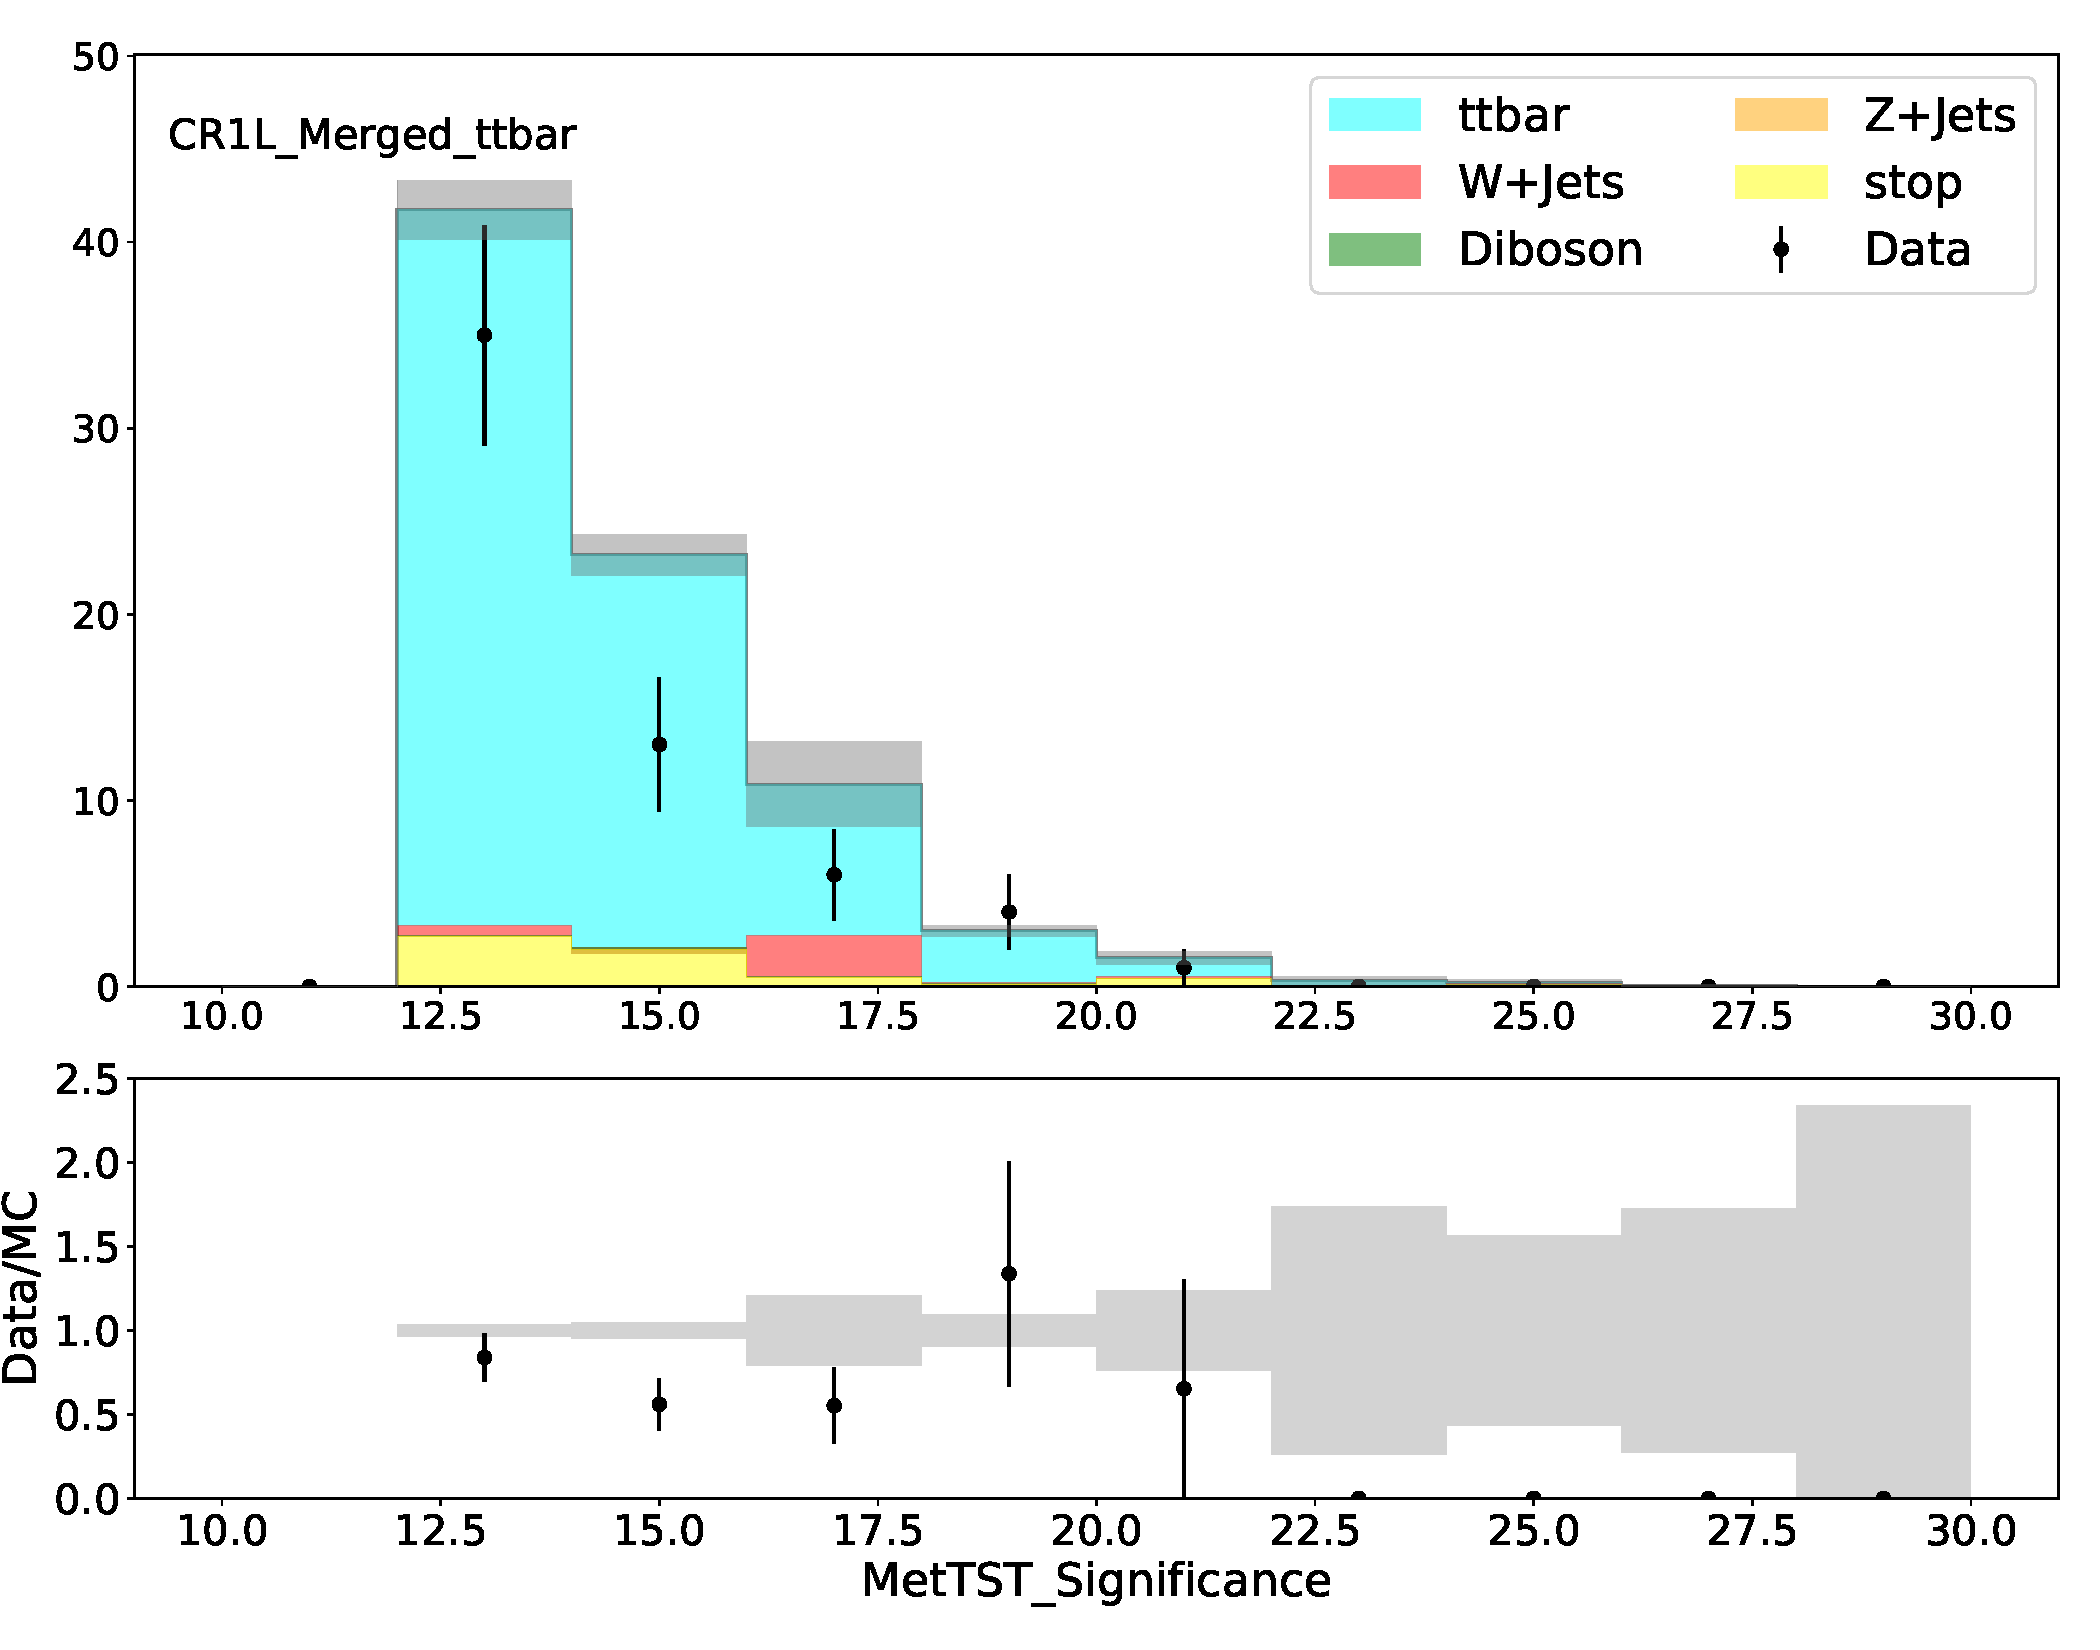
\includegraphics[width = 0.98\textwidth]{Figures/4/datamc/CR1L_Merged_ttbar/MetTST_Significance.pdf}
     \caption{\metsig}
     \end{subfigure}
     \begin{subfigure}{0.49\textwidth}
     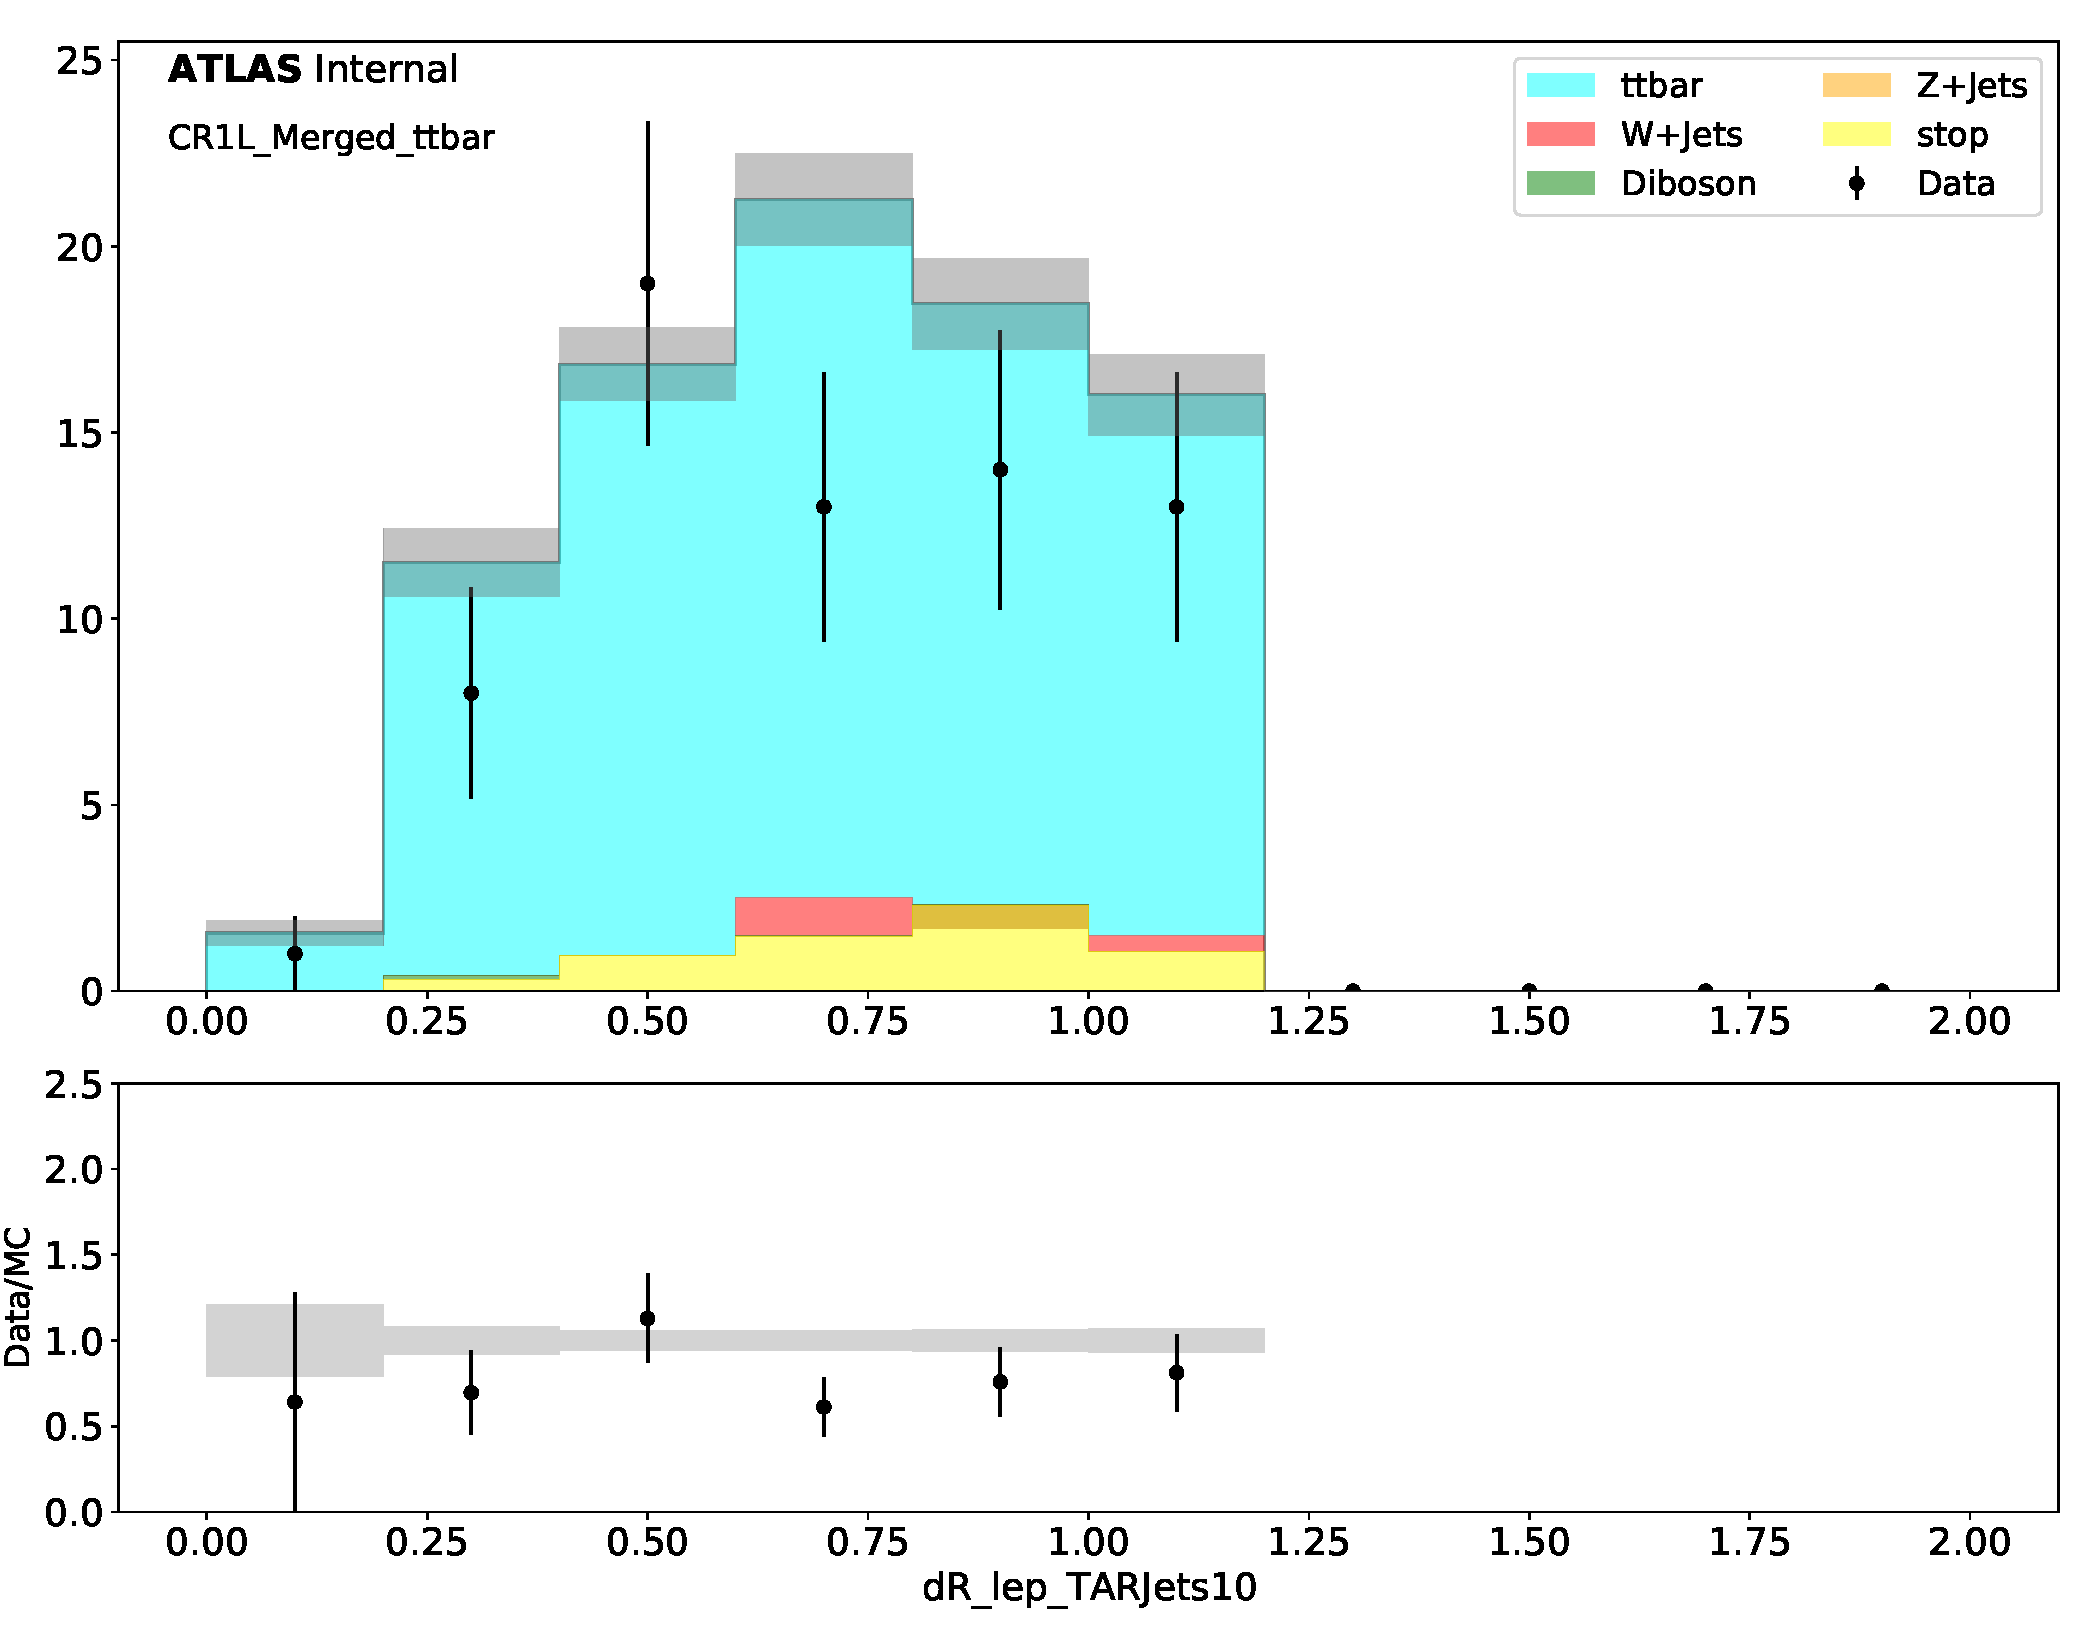
\includegraphics[width = 0.98\textwidth]{Figures/4/datamc/CR1L_Merged_ttbar/dR_lep_TARJets10.pdf}
     \caption{\drTARl}
     \end{subfigure}
     \begin{subfigure}{0.49\textwidth}
     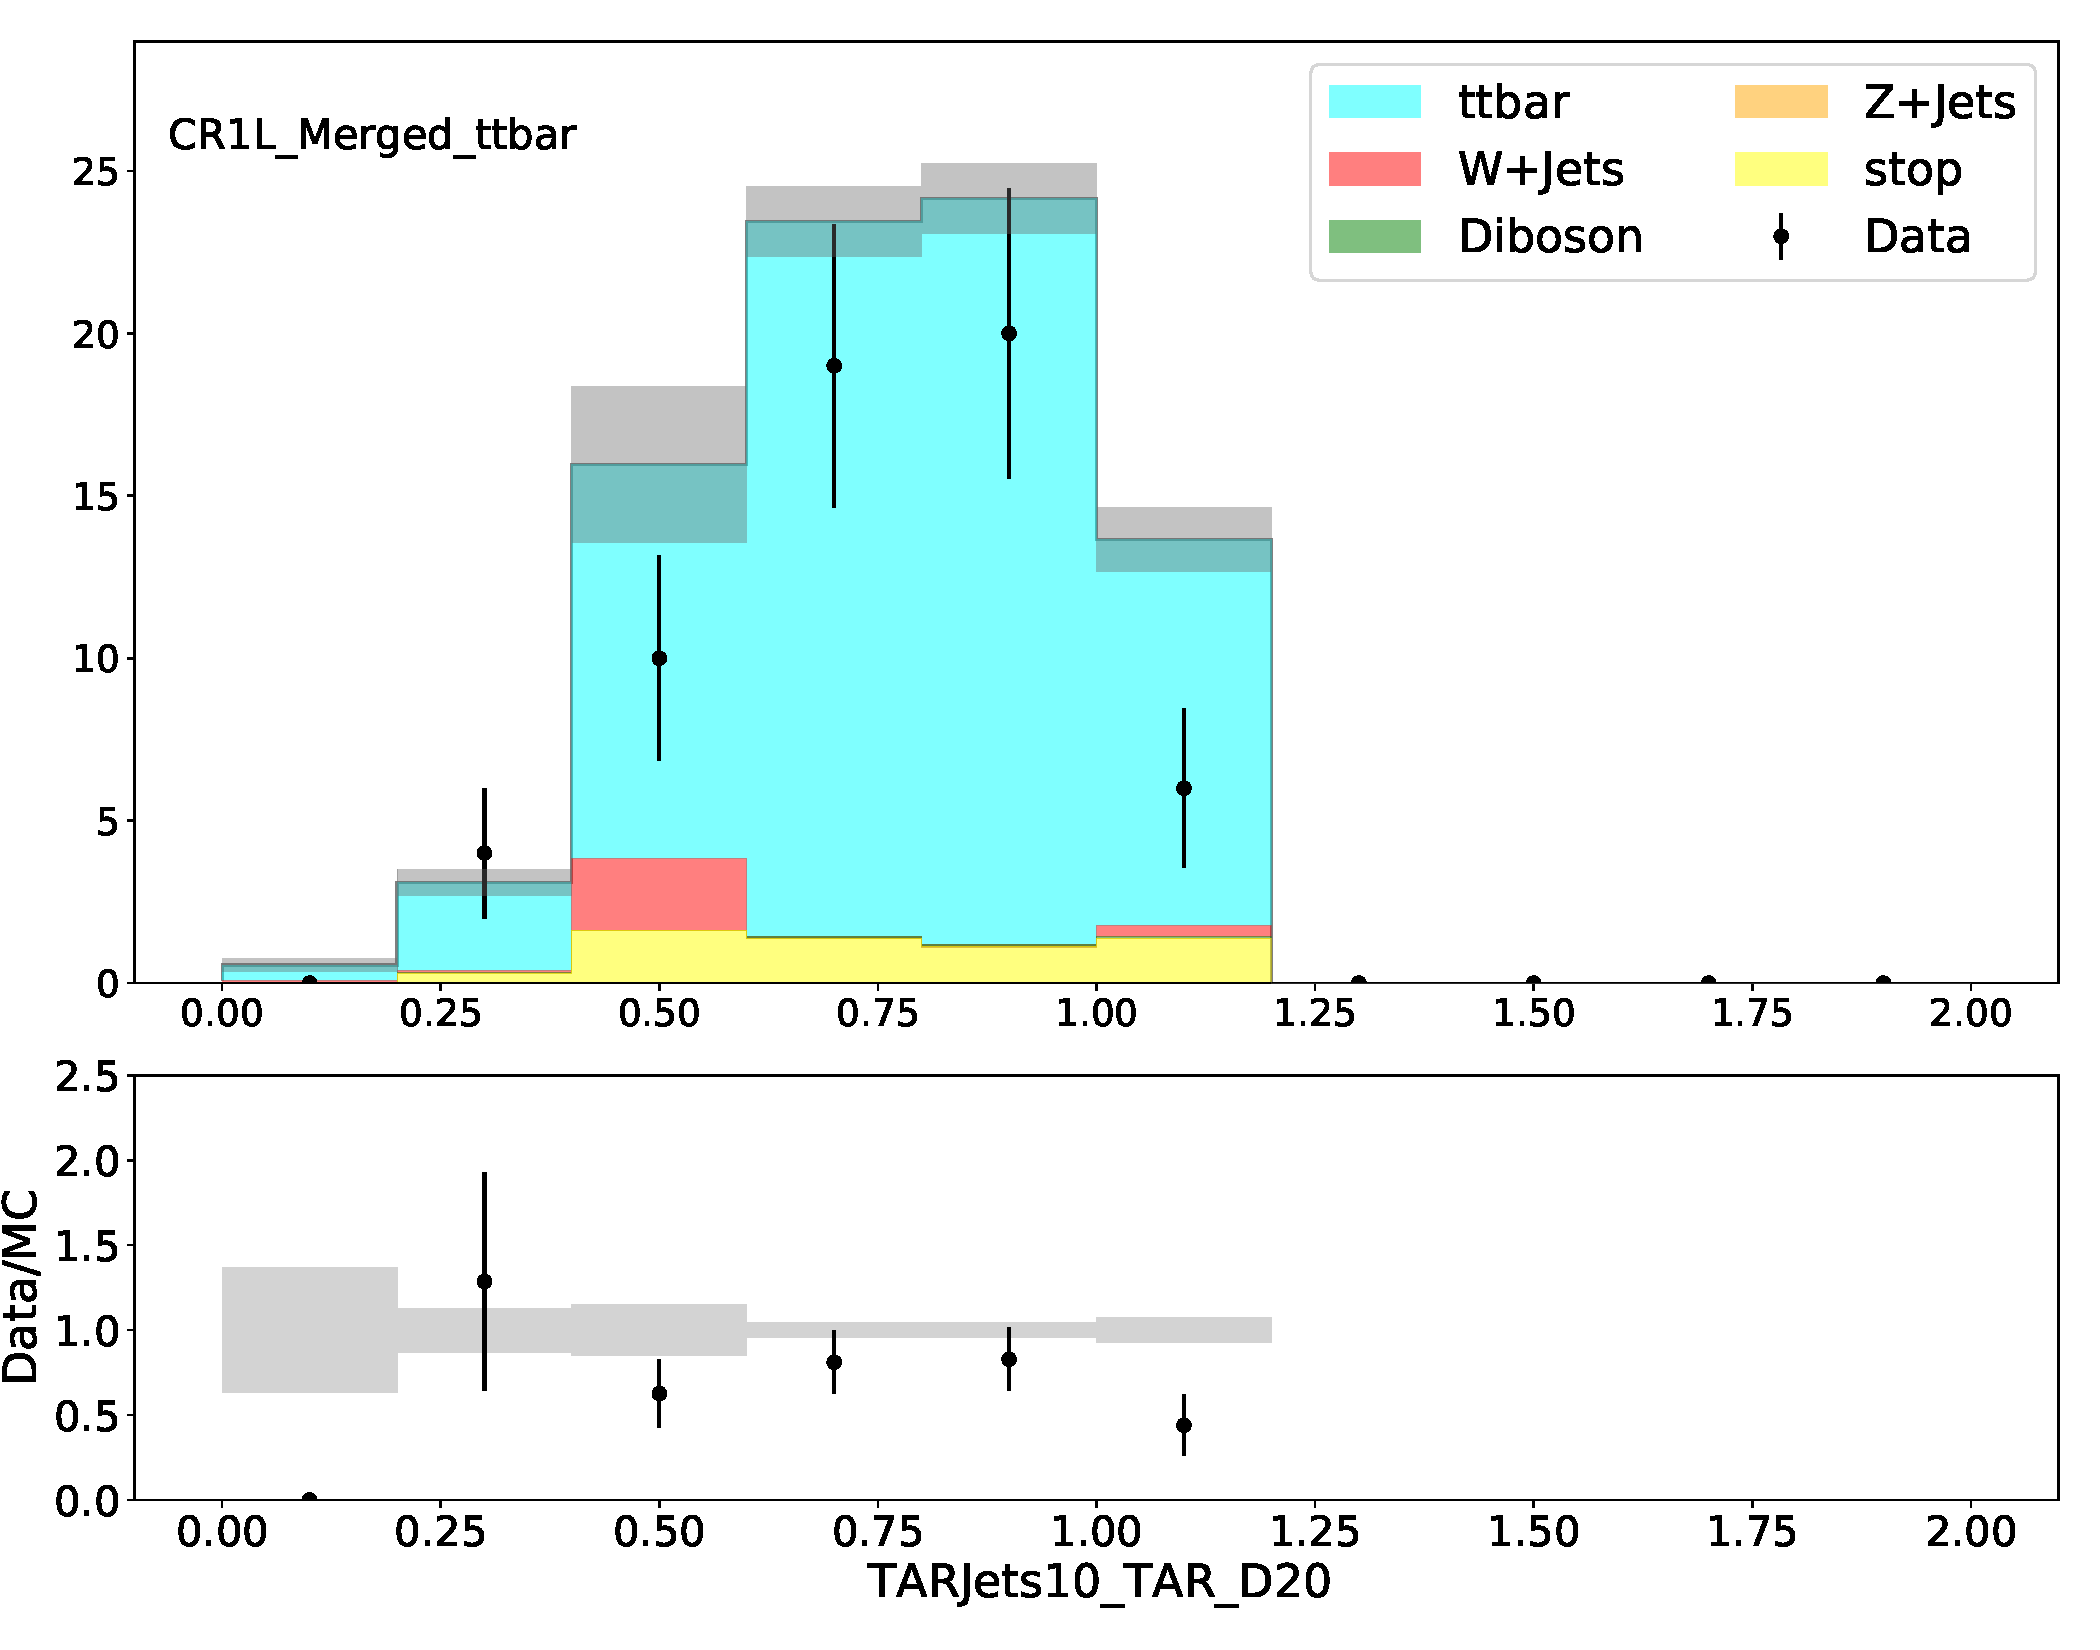
\includegraphics[width = 0.98\textwidth]{Figures/4/datamc/CR1L_Merged_ttbar/TARJets10_TAR_D20.pdf}
     \caption{\DtwoTAR}
     \end{subfigure}
     \begin{subfigure}{0.49\textwidth}
     \includegraphics[width = 0.98\textwidth]{Figures/4/datamc/CR1L_Merged_ttbar/MetTST_met.pdf}
     \caption{\met}
     \end{subfigure}

     \caption{Data-MC Comparisons in the \merged \ttbar control region.}
     \label{fig:Data_MC_CRbV_merged}
  \end{figure}

\begin{figure}[htbp]
  \centering
     \begin{subfigure}{0.49\textwidth}
     \includegraphics[width = 0.98\textwidth]{Figures/4/datamc/CR1L_Resolved_ttbar/mT_lep_met.pdf}
     \caption{\mtlepmet}
     \end{subfigure}
     \begin{subfigure}{0.49\textwidth}
     \includegraphics[width = 0.98\textwidth]{Figures/4/datamc/CR1L_Resolved_ttbar/WCand_m.pdf}
     \caption{\Wcandm}
     \end{subfigure}
     \begin{subfigure}{0.49\textwidth}
     \includegraphics[width = 0.98\textwidth]{Figures/4/datamc/CR1L_Resolved_ttbar/MetTST_Significance.pdf}
     \caption{\metsig}
     \end{subfigure}
     \begin{subfigure}{0.49\textwidth}
     \includegraphics[width = 0.98\textwidth]{Figures/4/datamc/CR1L_Resolved_ttbar/dRWl.pdf}
     \caption{\drWl}
     \end{subfigure}
     \begin{subfigure}{0.49\textwidth}
     \includegraphics[width = 0.98\textwidth]{Figures/4/datamc/CR1L_Resolved_ttbar/WCand_pt.pdf}
     \caption{\Wcandpt}
     \end{subfigure}
     \begin{subfigure}{0.49\textwidth}
     \includegraphics[width = 0.98\textwidth]{Figures/4/datamc/CR1L_Resolved_ttbar/MetTST_met.pdf}
     \caption{\met}
     \end{subfigure}

\caption{Data-MC Comparisons in the \resolved \ttbar control region.}
\label{fig:Data_MC_CRbV_resolved}
\end{figure}
\FloatBarrier
\subsection{\wjets Control Regions}
\begin{figure}[htbp]
  \centering
     \begin{subfigure}{0.49\textwidth}
     \includegraphics[width = 0.98\textwidth]{Figures/4/datamc/CR1L_Merged_WJets/mT_lep_met.pdf}
    \caption{\mtlepmet}
     \end{subfigure}
    \begin{subfigure}{0.49\textwidth}
     \includegraphics[width = 0.98\textwidth]{Figures/4/datamc/CR1L_Merged_WJets/TARJets10_mTAR0.pdf}
     \caption{\mTAR}
     \end{subfigure}
    \begin{subfigure}{0.49\textwidth}
     \includegraphics[width = 0.98\textwidth]{Figures/4/datamc/CR1L_Merged_WJets/MetTST_Significance.pdf}
     \caption{\metsig}
     \end{subfigure}
    \begin{subfigure}{0.49\textwidth}
     \includegraphics[width = 0.98\textwidth]{Figures/4/datamc/CR1L_Merged_WJets/dR_lep_TARJets10.pdf}
     \caption{\drTARl}
     \end{subfigure}
     \begin{subfigure}{0.49\textwidth}
     \includegraphics[width = 0.98\textwidth]{Figures/4/datamc/CR1L_Merged_WJets/TARJets10_TAR_D20.pdf}
     \caption{\DtwoTAR}
     \end{subfigure}
     \begin{subfigure}{0.49\textwidth}
     \includegraphics[width = 0.98\textwidth]{Figures/4/datamc/CR1L_Merged_WJets/MetTST_met.pdf}
     \caption{\met}
     \end{subfigure}

     \caption{Data-MC comparisons in the \merged \wjets control region.}
     \label{fig:Data_MC_CRdR_merged}
  \end{figure}

\begin{figure}[htbp]
  \centering
     \begin{subfigure}{0.49\textwidth}
     \includegraphics[width = 0.98\textwidth]{Figures/4/datamc/CR1L_Resolved_WJets/mT_lep_met.pdf}
     \caption{\mtlepmet}
     \end{subfigure}
     \begin{subfigure}{0.49\textwidth}
     \includegraphics[width = 0.98\textwidth]{Figures/4/datamc/CR1L_Resolved_WJets/WCand_m.pdf}
     \caption{\Wcandm}
     \end{subfigure}
     \begin{subfigure}{0.49\textwidth}
     \includegraphics[width = 0.98\textwidth]{Figures/4/datamc/CR1L_Resolved_WJets/MetTST_Significance.pdf}
     \caption{\metsig}
     \end{subfigure}
     \begin{subfigure}{0.49\textwidth}
     \includegraphics[width = 0.98\textwidth]{Figures/4/datamc/CR1L_Resolved_WJets/dRWl.pdf}
     \caption{\drWl}
     \end{subfigure}
     \begin{subfigure}{0.49\textwidth}
     \includegraphics[width = 0.98\textwidth]{Figures/4/datamc/CR1L_Resolved_WJets/WCand_pt.pdf}
     \caption{\Wcandpt}
     \end{subfigure}
     \begin{subfigure}{0.49\textwidth}
     \includegraphics[width = 0.98\textwidth]{Figures/4/datamc/CR1L_Resolved_WJets/MetTST_met.pdf}
     \caption{\met}
     \end{subfigure}

     \caption{Data-MC comparisons in the \resolved \wjets control region.}
     \label{fig:Data_MC_CRdR_resolved}
  \end{figure}

\FloatBarrier

\section{CR-SR Distribution Comparisons}
\label{section:CRSR}

\begin{figure}[htbp]
  \centering

    \begin{subfigure}{0.49\textwidth}
    \includegraphics[width = 0.98\textwidth]{Figures/4/CRSR/SR1L_Merged/dR_lep_TARJets10.png}
    \caption{Merged SR \drTARl}
    \end{subfigure}
    \begin{subfigure}{0.49\textwidth}
    \includegraphics[width = 0.98\textwidth]{Figures/4/CRSR/CR1L_Merged_ttbar/dR_lep_TARJets10.png}
    \caption{Merged CR \drTARl}
    \end{subfigure}
    \begin{subfigure}{0.49\textwidth}
    \includegraphics[width = 0.98\textwidth]{Figures/4/CRSR/SR1L_Merged/mT_lep_met.png}
    \caption{Merged SR \mtlepmet}
    \end{subfigure}
    \begin{subfigure}{0.49\textwidth}
    \includegraphics[width = 0.98\textwidth]{Figures/4/CRSR/CR1L_Merged_ttbar/mT_lep_met.png}
    \caption{Merged CR \mtlepmet}
    \end{subfigure}
    \begin{subfigure}{0.49\textwidth}
    \includegraphics[width = 0.98\textwidth]{Figures/4/CRSR/SR1L_Merged/MetTST_met.png}
    \caption{Merged SR \met}
    \end{subfigure}
    \begin{subfigure}{0.49\textwidth}
    \includegraphics[width = 0.98\textwidth]{Figures/4/CRSR/CR1L_Merged_ttbar/MetTST_met.png}
    \caption{Merged CR \met}
    \end{subfigure}


     \caption{Comparisons of kinematic variables between the \merged signal region and \ttbar control region. \textbf{Left column:} signal region, \textbf{Right column:} control region.}
     \label{fig:CRSR_merged}
  \end{figure}

  \begin{figure}[htbp]
    \centering

      \begin{subfigure}{0.49\textwidth}
      \includegraphics[width = 0.98\textwidth]{Figures/4/CRSR/SR1L_Resolved/dRWl.png}
      \caption{Resolved SR \drWl}
      \end{subfigure}
      \begin{subfigure}{0.49\textwidth}
      \includegraphics[width = 0.98\textwidth]{Figures/4/CRSR/CR1L_Resolved_ttbar/dRWl.png}
      \caption{Resolved CR \drWl}
      \end{subfigure}
      \begin{subfigure}{0.49\textwidth}
      \includegraphics[width = 0.98\textwidth]{Figures/4/CRSR/SR1L_Resolved/mT_lep_met.png}
      \caption{Resolved SR \mtlepmet}
      \end{subfigure}
      \begin{subfigure}{0.49\textwidth}
      \includegraphics[width = 0.98\textwidth]{Figures/4/CRSR/CR1L_Resolved_ttbar/mT_lep_met.png}
      \caption{Resolved CR \mtlepmet}
      \end{subfigure}
      \begin{subfigure}{0.49\textwidth}
      \includegraphics[width = 0.98\textwidth]{Figures/4/CRSR/SR1L_Resolved/MetTST_met.png}
      \caption{Resolved SR \met}
      \end{subfigure}
      \begin{subfigure}{0.49\textwidth}
      \includegraphics[width = 0.98\textwidth]{Figures/4/CRSR/CR1L_Resolved_ttbar/MetTST_met.png}
      \caption{Resolved CR \met}
      \end{subfigure}


       \caption{Comparisons of kinematic variables between the \resolved signal region and \ttbar control region. \textbf{Left column:} signal region, \textbf{Right column:} control region.}
       \label{fig:CRSR_resolved}
    \end{figure}


% The style of bibliography exemplified here is the "plain",
% normally used in science theses. This is shown
% by the entry {plain} below. Substitute the
% appropriate bibliography style. See also the
% PDF file "InformationOnBibliographyStyles" in this
% directory for more choices.

% The Bibliography file is a BibTex file named
% UVicThesis.bib and called below

	\TOCadd{Bibliography}
	\printbibliography

\end{document}
